% KIT grün
% C 100 M 0 Z 60 K 0
% R 0 G 150 B 130
%
% Color pages
% Anzahl            :  1  2  3  4  5   6   7   8   9  10  11  12  13  14  15  16  17  18  19  20
% Figure:           :  7 15 16 17 19  22  23  31  32  33  34  35  36  37  38  45  47  50  51  52
% Main Body page cnt: 37 66 68 71 84  89  90 109 110 113 118 119 123 125 126 148 150 159 160 162
% Total page count  : 49 78 80 83 96 101 102 121 122 125 130 131 135 137 138 160 162 171 172 174

% Total page count: 210 
% Main body page count: 198

% Doctoral thesis of Julian Moosmann using classicthesis
% TO DO
% Wave-particle-duality
% optical theorem
% diffraction limit
% introduce vector potential, retarded potential, 
% camera system
% Kohlrausch
% QM needed: Why
% scattering and absorption:discrete frequencies, dissipative effect, 
% meridional plane, figure, dipole radiation
% Rayleigh scattering
% plot of regularisation independence for pure-phase objects
% discussion tie {eq:linear-tie-phase},ctf condition for finite blur
% Schwinger parameters 
% phase shift ~ k * 1/k^2 ~ 1/k

\documentclass[
twoside,
openright,
titlepage,
numbers=noenddot,
headinclude,
fleqn,
% 1headlines,letterpaper,
a4paper,
footinclude=true,
cleardoublepage=empty,
abstractoff,
BCOR=5mm,
paper=a4,
fontsize=11pt,
british,ngerman,american,
%hidelinks=true,
%pdftex,pdfa,
]{scrreprt}
%********************************************************************
\setcapindent{0pt}
% ********************************************************************
%%%%%%%%%%%%%%%%%%%%%%%%%%%%%%%%%%%%%%%%%%%%%%%%%%%%%%%%%%%%%%%%%%%%%%
% classicthesis-config.tex 
%*********************************************************************

% ********************************************************************
% ********************************************************************
% 1. Configure classicthesis for your needs here, e.g., 
% remove "drafting" below 
% in order to deactivate the time-stamp on the pages
% ****************************************************************************
\PassOptionsToPackage{eulerchapternumbers,listings,
  %drafting,%
  pdfspacing,%floatperchapter,%linedheaders,%
  subfig,beramono,eulermath,parts,subfig}{classicthesis}
% ********************************************************************
% Available options for classicthesis.sty:
% drafting  parts nochapters linedheaders
% eulerchapternumbers beramono eulermath pdfspacing minionprospacing
% tocaligned dottedtoc manychapters listings floatperchapter subfig
% ********************************************************************

% ********************************************************************
% Triggers for this config
% ******************************************************************** 
\usepackage{ifthen}
\newboolean{enable-backrefs} % enable backrefs in the bibliography
\setboolean{enable-backrefs}{false} % true false
% ****************************************************************************

% ****************************************************************************
% ****************************************************************************
% 2. Personal data and user ad-hoc commands
% ****************************************************************************
\newcommand{\myTitleGerman}{Nichtlinearer Zugang f{\"u}r das inverse Problem der Phasenr{\"u}ckgewinnung aus Einzelmessungen der R{\"o}ntgenintensit{\"a}ten bei nur einem Propagationsabstand\xspace}
\newcommand{\myTitle}{Nonlinear approaches to the inverse problem
  of phase retrieval from single-measurement X-ray intensity data\xspace}
\newcommand{\myDegree}{Dipl.-Phys.\xspace}
\newcommand{\myName}{Julian Philipp Moosmann\xspace}
\newcommand{\myProf}{Prof. Dr. Tilo Baumbach\xspace}
\newcommand{\mySupervisor}{Dr. habil. Ralf Hofmann (Privatdozent)\xspace}
\newcommand{\myFaculty}{Physik\xspace}
\newcommand{\myDepartment}{Laboratorium für Applikationen der
  Synchrotronstrahlung (LAS)/ Institut für Photonenforschung und
  Synchrotronstrahlung (IPS)\xspace} 
\newcommand{\myUni}{Karlsruher Institut für Technologie (KIT)\xspace}
\newcommand{\myLocation}{Karlsruhe\xspace}
\newcommand{\myTime}{09.01.2015\xspace}
\newcommand{\myVersion}{version 0.1\xspace}
%\newcommand{\myOtherProf}{Prof. Dr. Yankeedoodle\xspace}

% ********************************************************************
% Setup, finetuning, and useful commands
% ********************************************************************
\newcounter{dummy} % necessary for correct hyperlinks (to index, bib, etc.)
\newlength{\abcd} % for ab..z string length calculation
\providecommand{\mLyX}{L\kern-.1667em\lower.25em\hbox{Y}\kern-.125emX\@}
% ********************************************************************

% ********************************************************************
% ********************************************************************
% New and renewed command
% ********************************************************************
\newcommand{\ie}{i.\,e.}
\newcommand{\Ie}{I.\,e.}
\newcommand{\eg}{e.\,g.}
\newcommand{\Eg}{E.\,g.} 
% Use \boldsymbol instead of \mathbf to allow for bold greek letter.
% The package bm is more carefull, but changes font of bodl letter.
% Use \mathbold to use bodl fonts from eulermath
%\renewcommand{\vec}[1]{\mathbf{#1}}
%\renewcommand{\vec}{\boldsymbol}
\renewcommand{\vec}{\mathbold}
% Vectors
\newcommand{\xt}{{\vec{x},t}}
% 1d
\newcommand{\kp}{k_\perp}
\newcommand{\xip}{\xi_{\perp}}
\newcommand{\xipm}{\abs{\xi_{\perp}}_m}
\newcommand{\xin}{\xi_{\mathrm{noise}}}
\newcommand{\xim}{\xi_{m}}
\newcommand{\xic}{\xi_{\mathrm{c}}}
\newcommand{\xib}{\xi_{\mathrm{b}}}
\newcommand{\xir}{{\xi_{r}}}
\newcommand{\xis}{{\xi_{s}}}
\newcommand{\xix}{{\xi_{x}}}
\newcommand{\xiy}{{\xi_{y}}}
\newcommand{\xiz}{{\xi_{z}}}
% Vectors: 2D
\newcommand{\np}{\nabla_\perp}
\newcommand{\inp}{\nabla_\perp^{-2}}
\newcommand{\npa}{\nabla_{\perp,\alpha}}
\newcommand{\vecdp}{\vec{d}_\perp}
\newcommand{\veckp}{\vec{k}_\perp}
\newcommand{\vecqp}{\vec{q}_\perp}
\newcommand{\vecrp}{\vec{r}_\perp}
\newcommand{\vecxp}{\vec{x}_\perp}
\newcommand{\vecsp}{\vec{s}_\perp}
\newcommand{\vecxip}{\vec{\xi}_\perp}
% Vectors: 3D
\newcommand{\vecd}{\vec{d}}
\newcommand{\vecj}{\vec{j}}
\newcommand{\veck}{\vec{k}}
\newcommand{\vecn}{\vec{n}}
\newcommand{\vecp}{\vec{p}}
\newcommand{\vecq}{\vec{q}}
\newcommand{\vecr}{\vec{r}}
\newcommand{\vecs}{\vec{s}}
\newcommand{\vecv}{\vec{v}}
\newcommand{\vecx}{\vec{x}}
\newcommand{\x}{\vec{x}}
\newcommand{\vecxi}{\vec{\xi}}
\newcommand{\vecA}{\vec{A}}
\newcommand{\vecB}{\vec{B}}
\newcommand{\vecE}{\vec{E}}
\newcommand{\vecD}{\vec{D}}
\newcommand{\vecH}{\vec{H}}
\newcommand{\vecM}{\vec{M}}
\newcommand{\vecP}{\vec{P}}
\newcommand{\vecS}{\vec{S}}
% Other
\newcommand{\BP}{\operatorname{BP}}
\newcommand{\FBP}{\operatorname{FBP}}
\newcommand{\adu}{\operatorname{ADU}}
\newcommand{\dqe}{\operatorname{DQE}}
\newcommand{\sgn}{\operatorname{sgn}}
\newcommand{\snr}[1]{\operatorname{SNR_{#1}}}
\newcommand{\NA}{\mathrm{NA}}
\newcommand{\Nrings}{N_{\circledcirc}}
\newcommand{\Npix}{N_\mathrm{x}}
\newcommand{\fwhm}{\operatorname{FWHM}}
\newcommand{\tie}{\operatorname{\textcolor{blue}{TIE}}}
\newcommand{\ctf}{\operatorname{\textcolor{red}{CTF}}}
\newcommand{\qp}{\operatorname{\textcolor{green}{QP}}}
\newcommand{\qpc}{\operatorname{\textcolor{black}{QP_\mathrm{con}}}}
\newcommand{\conv}{\operatorname{\ast\ast}}
\newcommand{\Prop}{\mathcal{P}}
\newcommand{\order}{\mathcal{O}}
\newcommand{\N}{\mathcal{N}}
\newcommand{\sigb}{\sigma_\mathrm{b}}
\newcommand{\sigs}{\sigma_\mathrm{s}}
\newcommand{\sig}[1]{\sigma_\mathrm{#1}}
%\newcommand{\Seik}{\mathcal{S}}
\newcommand{\e}[1]{\mathrm{e}^{#1}}
\newcommand{\me}{m_e}
\newcommand{\ed}{\rho_{e}}
\newcommand{\Iin}{I^{\mathrm{(in)}}}
\newcommand{\Ibin}{\bar{I}^{\mathrm{(in)}}}
\newcommand{\Psin}{ \Psi^\mathrm{(in)} }
\newcommand{\subn}[1]{_\mathrm{#1}}
\newcommand{\submax}{_\mathrm{max}}
\newcommand{\supin}{^\mathrm{(in)}}
\newcommand{\supl}{^{(l)}}
\newcommand{\env}{^\mathrm{(env)}}
\newcommand{\ho}[1]{^{(#1)}}
\newcommand{\hon}[1]{^{(\mathrm{#1})}}
\newcommand{\vecjin}{\vec{j}^{\mathrm{(in)}}}
\newcommand{\vecjsc}{\vec{j}^{\mathrm{(s)}}}
\newcommand{\hook}{k_h}
\newcommand{\dpo}{\delta\phi_0}
\newcommand{\dpom}{\abs{\delta{\phi_0}}_{\mathrm{max}}}
\newcommand{\delo}{\delta_\omega}
\newcommand{\fov}{\mathrm{FOV}}
\newcommand{\lmaxg}{{l_{\mathrm{max},g}}}
\newcommand{\lmaxphi}{{l_{\mathrm{max},\phi}}}
\newcommand{\nlo}[1]{\text{\small{NLO}}_{#1}}
\newcommand{\lc}{l_\mathrm{c}}
%\newcommand{\textsub}[1]{\ensuremath{_{\mbox{\footnotesize #1}}}}
%\newcommand{\sqrd}{{\textsuperscript 2}}
\newcommand{\rar}{\rightarrow}
\newcommand{\lar}{\leftarrow}
\newcommand{\ra}{\right\rangle}
\newcommand{\la}{\left\langle}
\newcommand{\ii}{\mathrm{i}}
% modulus
\newcommand{\abs}[1]{\left| #1 \right|} % for absolute value
\newcommand{\absn}[1]{| #1 |} % for absolute value when | too big
% average 
\newcommand{\avg}[1]{\left\langle #1 \right\rangle} % for average
\newcommand{\avgn}[1]{\langle #1 \rangle} 
% mean abs
\newcommand{\avgabs}[1]{\left\langle\left|#1\right|\right\rangle} 
\newcommand{\avgabsn}[1]{\langle|#1|\rangle} 
\newcommand{\mabs}[1]{\overline{#1}} 
% Fourier operator and symbol
\newcommand{\F}{\operatorname{\mathcal{F}}}
\newcommand{\iF}{\operatorname{\mathcal{F}^{-1}}}
\newcommand{\FO}[1]{\operatorname{\mathcal{F}#1}}
\newcommand{\ft}[1]{\widehat{#1}}
%\newcommand{\ft}[1]{\widetilde{#1}}
% angular averaged fft
\newcommand{\aft}[1]{\widetilde{#1}} 
% quasiparticle modification
\newcommand{\qpft}[1]{\widehat{#1}^{\mathrm{(QP)}}}
% derivatives and integral measures
\newcommand{\pd}{\partial}
\newcommand{\difd}{\mathrm{d}}
\newcommand{\Int}{\int\limits}
\newcommand{\intd}{\!\mathrm{d}}
\newcommand{\Intd}[1]{\!\mathrm{d}#1\,}
\newcommand{\Intdd}[1]{\!\mathrm{d^2}#1\,}
\newcommand{\Intddd}[1]{\!\mathrm{d^3}#1\,}
\newcommand{\const}{\mathrm{constant}}
% Matrices
\newcommand{\vv}[2]{\left(\begin{array}{c}#1\\#2\end{array}\right)}
\newcommand{\vvv}[3]{\left(\begin{array}{c}#1\\#2\\#3\end{array}\right)}
\newcommand{\mmmm}[4]{\left(\begin{array}{cc}#1&#2\\#3&#4\end{array}\right)}
% Other
\renewcommand{\hbar}{\hslash}
\newcommand{\bra}[1]{\left\langle#1\right|}
\newcommand{\ket}[1]{\left|#1\right\rangle}
% parentheses, brackets, and braces
\newcommand{\lp}{\left(}
\newcommand{\rp}{\right)}
\newcommand{\lrp}[1]{\left(#1\right)}
\newcommand{\lrb}[1]{\left[#1\right]}
\newcommand{\lrbr}[1]{\left\{#1\right\}}
\newcommand{\lb}{\left[}
\newcommand{\rb}{\right]}
\newcommand{\expsb}[1]{\exp\left[#1\right]}
\newcommand{\expb}[1]{\exp\left[#1\right]}
\newcommand{\expp}[1]{\exp\left(#1\right)}

\renewcommand{\floatpagefraction}{.7}
%*******************************************************
%********************************************************************
% Hyphenation
%*******************************************************
% use \hyphenchar\font=\string"7F for words containing hyphen
%\showhyphens{single-distance}
\hyphenation{
hard-X-ray 
sin-gle-dis-tance 
Rönt-gen 
mo-no-chro-ma-tic
par-ax-ial
Helm-holtz
Fou-ri-er
two-body
par-a-bolic
par-a-me-trised
Ang-ström-quel-le
mi-cro-to-mo-graphy
tech-nique
tech-niques
pe-ne-tra-tion
flu-o-res-cence
}
%*******************************************************

% ****************************************************************************
% 3. Loading some handy packages
% ****************************************************************************
% ******************************************************************** 
% Packages with options that might require adjustments
% ******************************************************************** 
\PassOptionsToPackage{utf8}{inputenc}	% latin9 (ISO-8859-9) = latin1+"Euro sign"
 \usepackage{inputenc}				
\PassOptionsToPackage{british,ngerman}{babel} %american
 \usepackage{babel}		
\PassOptionsToPackage{backend=biber,style=alphabetic,maxbibnames=9,maxnames=4}{biblatex}
\usepackage{biblatex}			
\bibliography{Bibliography}
\usepackage[]{csquotes}
% CREATES PROBLEM WHEN USING BIBLATEX
%\PassOptionsToPackage{square,numbers}{natbib}
% \usepackage{natbib}				
\PassOptionsToPackage{fleqn}{amsmath}% math environments and more by the AMS 
 \usepackage{amsmath}
% ******************************************************************** 
% General useful packages
% ******************************************************************** 
\PassOptionsToPackage{T1}{fontenc} % T2A for cyrillics
 \usepackage{fontenc} % alle 256 Zeichen des europäischen Zeichenvorrates in
 % T1-Kodierung.: Eingebunden wird die T1-Version der
 % Computer-Modern-Schriftsippe mit \usepackage[T1]{fontenc}. Dadurch
 % ist auch sichergestellt, dass in einem PDF Umlaute gefunden werden.
 % Sie umfasst 256 Zeichen und unterstützt damit sowohl die west- als
 % auch die osteuropäischen Sprachen mit lateinischem Alphabet.
\usepackage{scrhack} % fix warnings when using KOMA with listings package     
\usepackage{xspace} % to get the spacing after macros right  
\usepackage{mparhack} % get marginpar right
\usepackage{fixltx2e} % fixes some LaTeX stuff 
%\renewcommand*{\acsfont}[1]{\textssc{#1}} % for MinionPro
% ****************************************************************************

% ****************************************************************************
% 4. Setup floats: tables, (sub)figures, and captions
% ****************************************************************************
\usepackage{tabularx} % better tables
	\setlength{\extrarowheight}{3pt} % increase table row height
\newcommand{\tableheadline}[1]{\multicolumn{1}{c}{\spacedlowsmallcaps{#1}}}
\newcommand{\myfloatalign}{\centering} % to be used with each float for alignment
\usepackage{caption}
\captionsetup{format=hang,font=small}
\usepackage{subfig}
\usepackage{url}
% ****************************************************************************

% ****************************************************************************
% 5. Setup code listings
% ****************************************************************************
\usepackage{listings} 
%\lstset{emph={trueIndex,root},emphstyle=\color{BlueViolet}}%\underbar} % for special keywords
\lstset{language=[LaTeX]Tex,%C++,
    keywordstyle=\color{RoyalBlue},%\bfseries,
    basicstyle=\small\ttfamily,
    %identifierstyle=\color{NavyBlue},
    commentstyle=\color{Green}\ttfamily,
    stringstyle=\rmfamily,
    numbers=none,%left,%
    numberstyle=\scriptsize,%\tiny
    stepnumber=5,
    numbersep=8pt,
    showstringspaces=false,
    breaklines=true,
    frameround=ftff,
    frame=single,
    belowcaptionskip=.75\baselineskip
    %frame=L
} 
% ****************************************************************************
% ****************************************************************************
% 5./6. Additional package and options. Put here because hyperref
% package should be loaded as late as possible
% ****************************************************************************
%\usepackage{lmodern}
\usepackage{amssymb}
%\usepackage{bm} % bold math fonts !! changes appearance of bold fonts
%\usepackage{latexsym} % symbols already provided by the amsfonts & amssymb 
%\usepackage{mathabx} % more symbols: widehat, widecheck, etc
%\usepackage{yhmath}
\usepackage{mathtools}
\usepackage{mathrsfs}% calligrafic fonts for physicists
\usepackage{courier} % used for displaying code in text: \texttt{CODE}
%\usepackage{gensymb}
\usepackage{siunitx} %!! definitions(\celsius,...) in package gensymb collide with siunitx
\usepackage{textcomp} % removes warning: LaTeX Font Warning: Font
                      % shape `OMS/pplj/m/n' undefined 
%\usepackage[on]{auto-pst-pdf} % use psfrag with pdflatex
%\usepackage{psfrag} % replace labels in ps file
% global command option for psfragfig
\PassOptionsToPackage{process=auto}{pstool}%[process=none]%auto,all
 \usepackage{pstool}
\usepackage{classicthesis} 
%\usepackage{epstopdf} % to use pdflatex with eps images
%\graphicspath{ {./Images/} } % set image search path
%\usepackage[clearempty]{titlesec}
%\usepackage{todonotes}
% multible bibliographies
%\usepackage{multibib}
%\newcites{pub}{Publications}
%\usepackage{bibentry}
%\nobibliography*%{Bibliography}
\usepackage{tikz}
% Speed up compiling by externalising  tikz figures, not working
% \usepackage{pgfplots}
% \usetikzlibrary{external}
% \tikzexternalize[prefix=tikz/]
%\tikzset{external/force remake}
\usetikzlibrary{decorations.pathmorphing} % for decorations, wavy lines (snake)
%\usetikzlibrary{decorations.markings}% to draw tangent lines
%\usepackage{rotating} % for sidwaysfigure
%\usepackage{wrapfig} % wrap text around figure
\usepackage{caption}
\captionsetup{format=plain} 
\usepackage{chemfig}
\usepackage{enumitem}
%\usepackage{longtable}
%\usepackage{rotating}
\usepackage{tabu}
% ****************************************************************************
% 6. PDFLaTeX, hyperreferences and citation backreferences
% ****************************************************************************
% ********************************************************************
% Using PDFLaTeX
% ********************************************************************
\PassOptionsToPackage{hyperfootnotes=false,pdfpagelabels}{hyperref}
\usepackage{hyperref}  % backref linktocpage pagebackref
% most package must be loaded before hyperref to work properly except,
% e.g. amsref, cleveref
\pdfcompresslevel=9
\pdfadjustspacing=1 
% should avoid warnings: found pdf version 1.5 but at most version 1.4 allowed
\pdfminorversion=5
\PassOptionsToPackage{pdftex}{graphicx}
\usepackage{graphicx}

% acronym must be loaded after hyperref that hyperlinks to acronyms
% work properly. However it still doesn't. Otherwise use option
% 'nohyperlinks': wenn hyperref geladen ist, wird die Verlinkung
% unterbunden without compiling produces warning and the acronym links
% jump to the first page
\usepackage[printonlyused,nohyperlinks,
%smaller
]{acronym} % handling acronyms
 \renewcommand{\bflabel}[1]{{#1}\hfill} % fix the list of acronyms

% clever referencing. MUST BE LOADED AFTER HYPERREF
\usepackage[english,capitalise]{cleveref}
% Options: capitalise: for capital of all initial label, otherwise use
% \Cref and \Crefrange; cleveref: for full label names

% ********************************************************************
% Setup the style of the backrefs from the bibliography
% (translate the options to any language you use)
% ********************************************************************
\newcommand{\backrefnotcitedstring}{\relax}%(Not cited.)
\newcommand{\backrefcitedsinglestring}[1]{(Cited on page~#1.)}
\newcommand{\backrefcitedmultistring}[1]{(Cited on pages~#1.)}
\ifthenelse{\boolean{enable-backrefs}}%
{%
		\PassOptionsToPackage{hyperpageref}{backref}
		\usepackage{backref} % to be loaded after hyperref package 
		   \renewcommand{\backreftwosep}{ and~} % separate 2 pages
		   \renewcommand{\backreflastsep}{, and~} % separate last of longer list
		   \renewcommand*{\backref}[1]{}  % disable standard
		   \renewcommand*{\backrefalt}[4]{% detailed backref
		      \ifcase #1 %
		         \backrefnotcitedstring%
		      \or%
		         \backrefcitedsinglestring{#2}%
		      \else%
		         \backrefcitedmultistring{#2}%
		      \fi}%
}{\relax}    

% ********************************************************************
% Hyperreferences
% ********************************************************************
\hypersetup{%
    %draft,	% = no hyperlinking at all (useful in b/w printouts)
    colorlinks=true, 
    linktocpage=true, 
    pdfstartpage=3, 
    pdfstartview=FitV,%
    % uncomment the following line if you want to have black links (e.g., for printing)
    %colorlinks=false, linktocpage=false, pdfborder={0 0 0}, pdfstartpage=3, pdfstartview=FitV,% 
    breaklinks=true, 
    pdfpagemode=UseNone, 
    pageanchor=true, 
    pdfpagemode=UseOutlines,%
    plainpages=false, 
    bookmarksnumbered, 
    bookmarksopen=true, 
    bookmarksopenlevel=1,%
    hypertexnames=true, 
    pdfhighlight=/O, 
    % nesting=true,
    % frenchlinks,%
    urlcolor=webbrown, 
    linkcolor=RoyalBlue, 
    citecolor=webgreen, 
    % pagecolor=RoyalBlue,%
    %urlcolor=Black, linkcolor=Black, citecolor=Black, 
    %pagecolor=Black,%
    pdftitle={\myTitle},%
    pdfauthor={\textcopyright\ \myName, \myUni, \myFaculty},%
    pdfsubject={},%
    pdfkeywords={},%
    pdfcreator={pdfLaTeX},%
    pdfproducer={LaTeX with hyperref and classicthesis}%
}   

% ********************************************************************
% Setup autoreferences
% ********************************************************************
% There are some issues regarding autorefnames
% http://www.ureader.de/msg/136221647.aspx
% http://www.tex.ac.uk/cgi-bin/texfaq2html?label=latexwords you have
% to redefine the makros for the language you use, e.g., american,
% ngerman (as chosen when loading babel/AtBeginDocument)
% ********************************************************************

\makeatletter \@ifpackageloaded{babel}%
{%
  \addto\extrasamerican{%
    \renewcommand*{\figureautorefname}{Figure}%
    \renewcommand*{\tableautorefname}{Table}%
    \renewcommand*{\partautorefname}{Part}%
    \renewcommand*{\chapterautorefname}{Chapter}%
    \renewcommand*{\sectionautorefname}{Section}%
    \renewcommand*{\subsectionautorefname}{Section}%
    \renewcommand*{\subsubsectionautorefname}{Section}%
  }%
  \addto\extrasngerman{%
    \renewcommand*{\paragraphautorefname}{Absatz}%
    \renewcommand*{\subparagraphautorefname}{Unterabsatz}%
    \renewcommand*{\footnoteautorefname}{Fu\"snote}%
    \renewcommand*{\FancyVerbLineautorefname}{Zeile}%
    \renewcommand*{\theoremautorefname}{Theorem}%
    \renewcommand*{\appendixautorefname}{Anhang}%
    \renewcommand*{\equationautorefname}{Gleichung}%
    \renewcommand*{\itemautorefname}{Punkt}%
  }%

  % Fix to getting autorefs for subfigures right
  \providecommand{\subfigureautorefname}{\figureautorefname}%
    }{\relax}
\makeatother


%*******************************************************
\EndPreamble % needed for pstools (psfragfig), without execution fails
%*******************************************************
\begin{document}                    
\let\hbar=\hslash
%\AtBeginDocument{\let\hbar=\***@hslash}
\def\hyph{-\penalty0\hskip0pt\relax}
\hyphenchar\font=\string"7F
\frenchspacing
\raggedbottom
\selectlanguage{british}
\pagenumbering{roman}
\pagestyle{plain}
%********************************************************************
% Frontmatter
%*******************************************************
% Titlepage, front
%*******************************************************
\thispagestyle{empty}
\begin{titlepage}
\selectlanguage{ngerman}
  \begin{addmargin}[-1cm]{-3cm}
    \begin{center}
        \Large
        \hfill
        \vfill
        \begingroup
            %\color{Maroon}
            \spacedallcaps{{\myTitleGerman}} \\ %\bigskip
        \endgroup
        \vfill
        Zur Erlangung des akademischen Grades eines \\
        \medskip
        DOKTORS DER NATURWISSENSCHAFTEN \\
        \medskip
        von der Fakultät für Physik des \\
        \medskip
        Karlsruher Instituts für Technologie (KIT)\\
        \vfill
        genehmigte \\
        \vfill
        DISSERTATION \\
        \vfill
        \medskip
        von  \\
        \vfill
        \myDegree \myName \\ %\spacedlowsmallcaps{\myName}
        \medskip
        aus Bretten \\
        \vfill
%        \vfill                      
    \end{center}
    \hfill
    \vfill
    \noindent\bigskip
    Tag der mündlichen Prüfung: \myTime \\
    \bigskip
    Referent: \myProf \\
    \bigskip
    Korreferent: \mySupervisor
  \end{addmargin}       
\end{titlepage}   
%*******************************************************
% Titlepage, back
%*******************************************************
\thispagestyle{empty}
\hfill
\vfill
\noindent\myName: \textit{\myTitleGerman.} \myTitle. %\myDegree, 
\textcopyright\, \myTime
%\bigskip
%\noindent\spacedlowsmallcaps{Supervisors}: \\
%\myProf \\
%\myOtherProf \\ 
%\mySupervisor
%\medskip
%\noindent\spacedlowsmallcaps{Location}: \\
%\myLocation
%\medskip
%\noindent\spacedlowsmallcaps{Time Frame}: \\
%\myTime
\cleardoublepage

%*******************************************************
% Little Dirty Titlepage
%*******************************************************
\thispagestyle{empty}
%\pdfbookmark[1]{Titel}{title}
%*******************************************************
\begin{center}
    \spacedlowsmallcaps{\myName} \\ \medskip                        
    \begingroup
        %\color{Maroon}
        \spacedallcaps{\myTitle}
    \endgroup
\end{center}   
%*******************************************************
\cleardoublepage

%*******************************************************
% Abstract englisch
\selectlanguage{british}
%*******************************************************
%\renewcommand{\abstractname}{Abstract}
\pdfbookmark[1]{Abstract}{Abstract}
\begingroup
\let\clearpage\relax
\let\cleardoublepage\relax
\let\cleardoublepage\relax
\chapter*{Abstract}
\selectlanguage{british}

This thesis aims at the development of nonlinear approaches to the
inverse problem of phase retrieval from single\hyph measurement X-ray
intensity data.  Furthermore, intricacies of X-ray phase\hyph contrast
microtomography and its application for in vivo imaging in
developmental biology are considered.

In the framework of Fresnel theory, approaches to single-distance
phase retrieval that work beyond linearity are developed.  Starting
points are linear approximations to Fresnel theory.  On the one hand,
the \ac{tie} which is the imaginary part of the paraxial wave equation
and  valid in the limit of small propagation distances. On the other
hand, the \ac{ctf} which is limited to weakly varying phases but not
restricted to small propagation distances.

At large propagation distances, phase retrieval based on \ac{tie}
exhibits limited resolution since the corresponding filter in
transverse Fourier space acts as a low pass suppressing large
frequencies.  However, large propagation distances are required to
enhance the signal-to-noise ratio, in particular with respect to a
reduction of dose due to residual absorption.  Here a systematic
expansion of phase and intensity of the propagated wave front in
powers of propagation distance is proposed.  The expansion
coefficients are determined by appeal to full Fresnel theory, \ie{}
using both the imaginary and the real part of the paraxial wave
equation.  This yields a partial differential equation in the phase at
object exit.  Nonlinear corrections to the phase are evaluated
perturbatively in terms of the leading\hyph order estimate which is
given by the \ac{tie}\hyph phase.  While this approach improves phase
retrieval quantitatively, it cannot enhance spatial resolution owing
to the poor resolution of the \ac{tie} phase.

In order retrieve a highly resolved phase, we analyse the behaviour of
\ac{ctf} at strong phase variations as they occur in imaging of early
developmental stages of model organisms in development biology.  Under
upscaling of phase variations, intensity contrast exhibits a critical
phenomenon which is associated to a scaling symmetry, exact in the
limit of vanishing phase variations.  At finite phase variations, this
symmetry is explicitly broken by non-linear (and non-local)
propagation effects, causing a shift of  zeros crossings of the
Fourier transformed intensity.  However, below a critical value of
phase variations scaling symmetry is dynamically unbroken and the
positions of lifted zeros remain fixed.  Above phase variations of
order one, positions of lifted zeros exhibit critical behaviour and
start to move like order parameters in second\hyph order phase
transitions.  Moreover, below critical upscaling, the distribution of
information in Fourier space, which is concentrated between lifted
zeros, remains unchanged.  These two observations are exploited as
after a renormalisation of the propagated intensity a quasi-linear
relation between renormalised intensity and exit phase is restored,
which can be used input for \ac{ctf} phase retrieval.  This is
reminiscent to the ubiquitous concept of quasiparticles in condensed
matter and quantum field theory.  A significantly improved spatial
resolution of the quasiparticle approach compared to linear methods is
demonstrated on tomographic data of Xenopus frog embryos.

Furthermore, intricacies of tomographic reconstruction and related
artifacts are considered.  In particular, in the context of
phase-contrast data and local tomography large\hyph scale modulations
arise which considerably impair subsequent data processing and
analysis.  A means to mitigate such artifacts is demonstrated upon
reversing the order of phase retrieval and tomographic reconstruction.

The last part aims at the application of in vivo propagation\hyph
based phase contrast to image the early development of model organisms
in developmental biology.  Besides the effects of dose and the thus
required fine tuning of the experimental setup, developmental aspects
of the 'Xenopus laevis' model system are discussed.
 
\endgroup			
\vfill
\cleardoublepage

\pdfbookmark[1]{Kurzfassung}{Kurzfassung}
\begingroup
\let\clearpage\relax
\let\cleardoublepage\relax
\let\cleardoublepage\relax

\chapter*{Kurzfassung}
\selectlanguage{ngerman} 

Ziel dieser Arbeit ist die Entwicklung nichtlinearer Zugänge für das
inverse Problem der Phasenrückgewinnung aus Einzelmessungen der
Röntgenintensitäten bei nur einem Propagationsabstand.  Des weiteren
werden Fragestellungen im Bezug auf Röntgenphasenkontrast\hyph
Mikrotomographie und deren Anwendungen für die in vivo Bildgebung in
der Entwicklungsbiologie besprochen.

Im Rahmen der Fresneltheorie werden Erweiterungen gängiger Me\-thoden
der Phasenrückgewinnung aus einzelnen Intensitätsmessungen entwickelt.
Ausgangspunkt sind lineare Näherungen der Fresneltheorie.  Dies ist
zum einen die Intensitätstransportgleichung, wel\-che den Imaginärteil
der paraxialen Wellengleichung darstellt und im Limes kleiner
Propagationsabstände gültig ist.  Zum anderen die
Kontrasttransferfunktion, welche im Grenzfall schwach variierender
Phasen angewandt wird, jedoch nicht auf kleine Propagationsabstän\-de
be\-schränkt ist.

Bei großen Propagationsabständen ist die Phasenrückgewinnung unter
Verwendung der Intensitätstransportgleichung auflösungslimitiert, da
der entsprechende Filter im transversalen Fourierraum als Tiefpass
wirkt und hohe Frequenzen unterdrückt.  Große Propagationsabstände
sind aber erforderlich um ein gutes Signal\hyph Rausch\hyph Verhältnis
zu erhalten.  Insbesondere im Hinblick auf eine Begrenzung der
Strahlendosis aufgrund residualer Absorption.  Hier wird ein An\-satz
gewählt welcher Phase und Intensität der propagierten Wellenfront in
Potenzen des Propagationsabstands entwickelt.  Die
Entwicklungskoeffizienten werden dann mithilfe der vollen
Fresneltheorie bestimmt, d.h. unter Zuhilfenahme von Imaginär- und
Realteil der paraxialen Wellengleichung.  Damit erhält man eine
nichtlineare partielle Differentialgleichung in der Phase bei
Objekt\hyph Austritt.  Korrekturen nichtlinear Ordnung zur Phase
werden im Sinne einer Störungstheorie durch das Ergebnis zur ersten
Ordnung ermittelt, welches mit dem der Intensitätstransportgleichung
identisch ist.  Dieses Zugang führt zu einer quantitativen
Verbesserung der zurückgewonnenen Phasenkarte, erhöht jedoch nicht
deren räumliches Auflösungsvermögen gegenüber der linearen Ordnung.

Um dennoch eine hochaufgelöste Phasenkarte bei großen Abständen zu
gewinnen wird das Verhalten der Kontrasttransferfunktion bei starken
Phasenvariationen betrachtet wie sie z.B. bei der Untersuchung früher
Embryonalstadien von Modellorganismen in der Entwicklungsbiologie
auftreten.  Unter einer Hochskalierung der Phasenvariationen wird im
propagierten Intensitätskontrast ein kritisches Phänomen beobachtet.
Dieses steht im Zusammenhang mit einer im Limes verschwindender
Phasenvariationen exakten Skalierungssymmetrie.  Aufgrund nichtlinear
(und nichtlokaler) Propagationseffekte wird diese Symmetrie explizit
gebrochen, was ein Anheben der Nullstellen der Fouriertransformierten
Intensität bei endlichen Phasenvariationen zur Folge hat.  Unterhalb
eines kritischen Wertes der Pha\-sen\-va\-ri\-a\-tio\-nen ist die
Skalierungssymmetrie jedoch dynamisch nicht gebrochen und die Position
der angehobenen Nullstellen bleibt unverändert.  Oberhalb von
Phasenvariationen der Ordnung eins wird ein kritisches Verhalten der
Nullstellenpositionen beobachtet, welche beginnen fort zu laufen wie
Ordnungsparameter in Phasenübergängen zweiter Ordnung.  Des weiteren
bleibt unterhalb kritischer Werte der Phasenvariationen die zwischen
den Nullstellen im Fourierraum konzentrierte Verteilung der
Information erhalten.  Unter Ausnutzung dieser beiden Phänomene erhält
man nach einer geeigneten Re\-nor\-mier\-ung der propagierten
Intensität eine quasilineare Beziehung zwischen Phasenkarte in der
Objektebene und renormierter Intensität, welche die
Phasenrückgewinnung mittels der linearen Kontrasttransferfunktion
gestattet.  Dies ähnelt dem Konzept von Quasiteilchen in der Theorie
der kondensierten Materie oder Quantenfeldtheorie.  An tomografische
Daten von Froschembryonen wird eine deutlich erhöhte räumliche
Auflösung des Quasiteilchen\hyph Zugangs gegenüber linearen Methoden
demonstriert.

Im weiteren wird auf Probleme bei der tomografischen Rekonstruktion
und diesbezüglicher Artefakte eingegangen.  Insbesondere im
Zusammenhang mit Phasenkontrastdaten und lokaler Tomografie treten
großskalige Variationsartefakte auf welche die nachfolgende
Datenverarbeitung und -analyse erheblich erschweren.  Zur Reduktion
solche Artefakte wird hier unter anderem eine Umkehrung der
Reihenfolge von Phasenrückgewinnung und tomografischer Rekonstruktion
betrachtet.
 
Im letzten Abschnitt wird die Röntgenphasenkontrast\hyph
Mikrotomographie für die vierdimensionale Bildgebung der frühen
Entwicklung in lebenden Modellorganismen angewandt.  Neben den
Auswirkungen der Strahlendosis und der damit einhergehenden
notwendigen Optimierung des experimentellen Setups, wird auf
entwicklungsbiologische Fragestellungen im Froschsystem 'Xenopus
laevis' eingegangen.

\endgroup			
\vfill
\cleardoublepage
\selectlanguage{british}
%*******************************************************
% Publications
%*******************************************************
\pdfbookmark[1]{Publications}{publications}
\chapter*{Publications}

Some ideas and figures have appeared previously in the following
publications:
\begin{itemize}[leftmargin=*]

\item[] J.~Moosmann, A.~Ershov, V.~Weinhardt, T.~Baumbach,
  M.~S.~Prasad, C.~LaBonne, X.~Xiao, J.~Kashef \&
  R.~Hofmann. Time-lapse X-ray phase-contrast microtomography for
  \emph{in vivo} imaging and analysis of morphogenesis. \emph{Nature
    Protocols} {\textbf 9}, 294 (2014).

\item[] J.~Moosmann, A.~Ershov, V.~Altapova, T.~Baumbach,
  M.~S.~Prasad, C.~LaBonne, X.~Xiao, J.~Kashef \& R.~Hofmann. X-ray
  phase-contrast \emph{in vivo} microtomography probes new aspects of
  \emph{Xenopus} gastrulation. \emph{Nature} {\textbf 497}, 374 (2013).

\item[] J.~Moosmann, V.~Altapova, L.~Helfen, D.~Hänschke,
  R.~Hofmann \& T.~Baumbach. High-resolution X-ray phase-contrast
  tomography from single-distance radiographs applied to developmental
  stages of \emph{Xenopus laevis}. \emph{J. Phys.: Conf. Ser.} {\textbf
    425}, 192003 (2013).

\item[] J.~Moosmann, V.~Altapova, D.~Hänschke, R.~Hofmann \&
  T.~Baumbach.  Non-Linear, noniterative, single-distance phase
  retrieval and developmental biology. \emph{AIP Conf. Proc.} {\textbf
    1437}, 57 (2012).

\item[] R.~Hofmann, J.~Moosmann \& T.~Baumbach. Criticality in
  single-distance phase retrieval. \emph{Opt. Express} {\textbf 19}, 25881
  (2011).

\item[] J.~Moosmann, R.~Hofmann \& T.~Baumbach. Non-Linear,
  single-distance phase retrieval and Schwinger regularization.
  \emph{Phys. Status Solidi A} {\textbf 208}, 2511 (2011).

\item[] J.~Moosmann, R.~Hofmann \& T.~Baumbach. Single-distance phase
  retrieval at large phase shifts. \emph{Opt. Express} {\textbf 19}, 12066
  (2011).

\item[] J.~Moosmann, R.~Hofmann, A.~V.~Bronnikov \&
  T.~Baumbach. Nonlinear phase retrieval from single-distance
  radiograph. \emph{Opt.  Express} {\textbf 18}, 25771 (2010).

% \item[] X.~Yang, R.~Hofmann, R. Dapp, T. van de Kamp, T. dos Santos
%   Rolo, X. Xiao, J. Moosmann, J. Kashef, T. Baumbach, \& R.  Stotzka.
%   TV-based Conjugate Gradient Method and Discrete L-curve for Few-view
%   CT Reconstruction of X-ray in vivo Data.  In review at
%   \emph{Opt. Express} (2014).

% \item[] V.~Altapova, L.~Helfen, A.~Myagotin, D.~Hänschke,
%   J.~Moosmann, J.~Gunneweg, T.~Baumbach. Phase contrast laminography
%   based on Talbot interferometry. \emph{Opt. Express} {\textbf 20}, 6496
%   (2012).

% \item[] V.~Altapova, J.~Butzer, T.~d.~S.~Rolo, P.~Vagovic, A.~Cecilia,
%   J.~Moosmann, J.~Kenntner, J.~Mohr, D.~Pelliccia, V.~F.~Pichugin,
%   T.~Baumbach. X-ray phase-contrast radiography using a filtered white
%   beam with a grating interferometer. \emph{Nucl. Instrum.  Meth. A}
%   {\textbf 648}, 42 (2011).

\end{itemize}

\cleardoublepage

%*******************************************************
% Table of Contents
%*******************************************************
%\phantomsection
\refstepcounter{dummy}
\pdfbookmark[1]{\contentsname}{tableofcontents}
\setcounter{tocdepth}{2} % <-- 2 includes up to subsections in the ToC
\setcounter{secnumdepth}{3} % <-- 3 numbers up to subsubsections
\manualmark
\markboth{\spacedlowsmallcaps{\contentsname}}
{\spacedlowsmallcaps{\contentsname}}
\tableofcontents 
\automark[section]{chapter}
\renewcommand{\chaptermark}[1]{\markboth{\spacedlowsmallcaps{#1}}
  {\spacedlowsmallcaps{#1}}}
\renewcommand{\sectionmark}[1]{\markright{\thesection\enspace\spacedlowsmallcaps{#1}}}

%********************************************************************
% Mainmatter
%*******************************************************
% use \cleardoublepage here to avoid problems with pdfbookmark
\cleardoublepage
\pagenumbering{arabic}
%\setcounter{page}{1}
%************************************************

%%%%%%%%%%%%%%%%%%%%%%%%%%%%%%%%%%%%%%%%%%%%%%%%%%%%%%%%%%%%%%%%%%%%%%
%% CHAPTER
%%%%%%%%%%%%%%%%%%%%%%%%%%%%%%%%%%%%%%%%%%%%%%%%%%%%%%%%%%%%%%%%%%%%%%

\chapter{Introduction}
\label{cha:intro}

The discovery of X-rays represents a milestone in the history of
imaging.  It opened up the possibility to visualise internal
structures of objects that had hitherto been eluded human
perception. % imperceptible to the human eye.
Already in 1893 Helmholtz forecasted a high penetration ability and
small refrangibility (refractivity) for propagating electromagnetic
fields with wave lengths of atomic order.  Prior to Röntgen's
discovery of X-rays in 1895, Hertz and Lenard have noted the existence
of metal penetrating rays producing photographic impressions
\cite{Glasser1934}.  However, it was Röntgen who systematically
studied the penetrating power of X-rays \cite{Roentgen1896} that led
to immediate applications.  The first clinical X-ray experiment was
performed shortly after Röntgen's announcement \cite{Spiegel1995}.
Since then X-rays have been beneficially applied across disciplines.
% \footnote{Apart from more harmful than useful applications such as
%   shoe-fitting fluoroscope; not to mention the atomic bomb.}

The characteristic spectrum of secondary X-rays emitted from materials
irradiated with hard X- or gamma rays was discovered by Barkla
\cite{Barkla1904}.  Peculiar to a particular substance, this
fluorescent radiation is used for elemental and chemical analysis in
X-ray spectroscopy.
% The emission of secondary X-rays from materials irradiated with a
% beam of high-energy X-rays discovered by Barkla \cite{Barkla1904}.
% The spectrum of secondary X-rays is characteristic for each element
% and
Furthermore, Barkla discovered the polarisation of X-rays
\cite{Barkla1905}.  This and diffraction experiments on a single slit
supported a wave-like interpretation of the X-radiation and suggested
its wave length to be in the order of \SI{e-10}{m}
\cite{Sommerfeld1912}.

Another remarkable feat was the discovery of X-ray diffraction through
crystals by Laue in 1912 \cite{Friedrich1913}.  Attributing the
observed diffraction pattern to the interference of waves which were
diffracted by the crystal's atomic lattice, Bragg connected the
macroscopic and the atomic (world) \cite{Bragg1913a}.  Allowing to
deduce the local position of atoms in a crystal, this did not only
elucidate the wave nature of X-rays, but marks the advent of modern
X-ray crystallography, which aims to understand the structure of
matter.  X-ray crystallography made it possible to determine the
atomic structure of simple minerals, sophisticated materials such as
graphene, or highly complex molecules and proteins such as \ac{dna},
enzymes, transcription factors, the components of the cytoplasm and
the cellular machines, and viruses.  The need for appropriately sized
crystals is mitigated by powder diffraction using polycrystalline
samples \cite{Debye1916,Hull1917} or by fibre diffraction in the case
of oriented fibres such as \ac{dna} \cite{Polanyl1921}.
% Fiber diffraction deals with samples showing uniaxial symmetry wich
% aggravates the determination of the crystallographic structure
% \cite{Polanyl1921}.
The X-ray image of \ac{dna}, that was recorded by Franklin in 1952
\cite{FranklinGosling1953} and which inspired Crick and Watson to
their \ac{dna} model of the double helix \cite{Watson1953}, was
acquired by means of fibre diffraction.  Another versatile method to
investigate a variety of materials, including non-crystalline solids
or even liquids, is small\hyph angle X-ray scattering (SAXS).  It
exploits the elastic scattering of X-rays by colloidal structures
which are due to electron density inhomogeneities within the sample
\cite{GlatterKratky1982}.

In 1905, explaining the photoelectric effect, Einstein introduced the
concept of a photon as a quantum of light \cite{Einstein1905}.  His
findings suggest a corpuscular interpretation of X-rays, confirmed by
the observation of (inelastic) scattering of X-rays from electrons by
Compton in 1923 \cite{Compton1923}.  X-ray absorption spectroscopy
(XAS) exploits the photoelectric effect to probe the transition of
photoelectrons from core electronic states (usually K-, L-, and
M-edges) to excited states just below or unbound states in the
continuum.  %Spectroscopy is employed atomic and molecular physics.
The former is known as \ac{XANES}, and the latter as \ac{EXAFS}.
Measuring the \ac{XASF}, which comprises \ac{XANES} and \ac{EXAFS},
allows to deduce information about the local atomic
environment and the chemical state in terms of the numbers, types, and
distances of neighbouring atoms, their coordination numbers, or
electronic structures \cite{KoningsbergerPrins}.

While in radiation therapy they are also employed to treat cancer,
X-rays are mostly applied in medical imaging where their use can be
considered revolutionary. Conventional projection radiography provides
a two-dimensional, superimposed representation of internal structures
of the human body.  It visualises strongly absorbing tissues such as
bones, gall or kidney stones, but also contrast variations between air
and the soft pulmonary tissue of the lungs or those introduced by
cavities in carious teeth.  In Fluoroscopy intensity contrast is
enhanced by means of contrast agents.  This enables to investigate the
gastrointestinal tract or to visualise veins and arteries of the
cardiovascular system or the cerebral spinal fluid (angiography).  As
a three-dimensional extension of these imaging strategies, X-ray
\acl{ct} has become indispensable for medical imaging.

Tomography was invented to acquire more than a mere projection of the
human body.  Here, cross-sectional images of the inside of the body
are obtained, allowing for a three-dimensional representation of the
body's internal parts.  Practical implementations of \acl{ct} were
independently developed by Hounsfield \cite{Hounsfield1973} and
Oldendorf \cite{Oldendorf1961}.  Mathematically, the problem of
reconstructing an object from a set of its projections (line
integrals) was already solved by Radon in 1917 \cite{Radon1917}; and
45 years later, simultaneous to the work of Hounsfield, by Cormack
\cite{Cormack1963,Cormack1964} being unaware of Radon's work.
Rapidly X-ray \acf{ct} turned into an invaluable tool for medical
diagnostics as well as industrial imaging, where \ac{ct} scanners have
found a broad scope of commercial applications as \eg{} in metrology,
non-intrusive inspection, non-destructive testing, or transport
security.
% revolutionizing medical diagnostics.

Nowadays, modern synchrotron radiation facilities range among the most
technologically complex scientific machines in the world
\cite{Wilson1996}.  Devoted to the production of X-rays of extreme
brilliance and coherence only, these facilities serve the scientific
and applied community as sophisticated tools to explore the structure
and dynamics of matter.
% down to the molecular and atomic level and at femtosecond
% resolution; from materials science to biology, chemistry,
% environmental and planetary science, and fundamental physics.
Such X-ray sources allow to acquire data of unprecedented quality in
terms of spatiotemporal resolution and intensity contrast.  This,
combined with recent developments in detector technologies
\cite{Martin2006} and a growing computational infrastructure, has
advanced the field of X-ray imaging tremendously.

In a typical imaging experiment, a quasi-parallel photon beam impinges
on a sample whose electron density distribution is described by the
refractive index.  An imprint is left on the photon beam by the sample
in terms of local amplitude and phase modulations of the transmitted
wave front.  The induced modulations are given by line integrals of
the refractive index along the photon path and thus represent
projections of the electron density.  The exiting wave front then
propagates towards the detector.  This situation is well described by
Fresnel diffraction theory \cite{HuygensYoungFresnel}.

For materials with high atomic number exhibiting strong absorption,
the object information is encoded in local amplitude modulations of
the exit wave.  In the absence of propagation effects the amplitude is
determined by the square root of the intensity.  Materials of low
atomic number and number density, such as polymers or soft biological
tissue, exhibit a weak attenuation of hard X-rays only, and absorption
contrast is poor.  However, phase shifts of the exit wave front
imparted by such samples are still sizable.  Therefore we are obliged
to appeal to the information contained in the phase variations of the
exit wave.  Already visible light oscillates at frequencies in the
order of \SI{e14}{Hz}, %X-rays: \SIrange{e16}{e19}{Hz}
which is far beyond the read-out rates of current detectors.  Only the
temporal average of the squared modulus of the electromagnetic wave is
accessible, rendering a direct measurement of the phase of a wave
field impossible.

In optical microscopy, this problem was solved by Zernike who invented
phase contrast microscopy \cite{Zernike1942a, Zernike1942b,
  Zernike1955}.  Upon conversion of specimen-induced phase shifts into
brightness variations, Zernike could reveal structures invisible to
traditional bright field microscopes.  Nowadays, this technique is
also employed in X-ray microscopes at synchrotron facilities
\cite{Schmahl1994}.  Besides Zernike phase contrast, a diversity of
interferometric phase-contrast techniques were developed to deduce the
local phase variations of an X-ray wave front in the transverse plane,
\eg{} crystal interferometry \cite{BonseHart1965}, analyser-based or
diffraction-enhanced imaging \cite{Chapman1997}, grating
interferometry \cite{Momose2003}, coded apertures \cite{Olivo2008} or
edge illumination \cite{Pelliccia2013}.  An instrumentally simpler
approach to sense the phase appeals to the self-interference of
propagating (coherent) X-rays, an effect that already Röntgen sought
after \cite{Roentgen1896}.  Yet, it was not before the advent of
modern synchrotrons, producing highly coherent beams of X-rays, that
advantage could be taken of such self-interference effects, making
propagation-based phase-contrast possible
\cite{Snigirev1995,Wilkins1996,Paganin1998}.  Distortions in the exit
wave front result in locally diffracted light rays which, by
free-space propagation over a distance in the range of decimetres,
start to interfere; and intensity contrast emerges.

Apart from an enhanced sample-to-detector distance and demands on beam
coherence, the setup of a propagation-based phase-contrast experiment
is practically identical to that of conventional absorption contrast
radiography.  It is free from additional optics such as crystals or
gratings.  Neither does it require a scanning or stepping procedure as
in diffraction-enhanced imaging or grating interferometry,
respectively, nor the meticulous alignment and stability of a crystal
interferometer.  Thus, the technique is dose efficient and
instrumentally simple, and requires a single intensity measurement at
a single distance only.  Optionally, measurements at several distances
can be acquired to improve image quality or to overcome restrictions
posed by reconstruction algorithms.  Therefore, propagation-based
phase-contrast imaging has evolved into a standard technique at modern
synchrotron.

% Moreover, the real part of the refractive index starts to dominate
% the imaginary part of the refractive with increasing photon energy
% further diminishing the absorption contrast.  Invoking the coherence
% properties of modern imaging beamline enables phase variations of
% the transmitted wave front to become visible as intensity variations
% by means of free-space propagation induced self-interference
% \cite{Snigirev1995, Wilkins1996, Paganin1998}.

Resorting to propagation-based phase contrast, the retrieval of the
phase of the exiting wave front from the measured intensity is a
precursor for two- or three-dimensional image analysis.  In Fresnel
theory, the exact inversion of the non-local and non-linear relation
between phase and intensity represents an insurmountable obstacle.
The problem of phase retrieval appears in various other fields such as
electron and optical microscopy, wave front sensing, crystallography,
or astronomy.  Numerous approaches were devised to address this issue.
Adaptive optics \eg{} measure and correct for distortions in the wave
front.  Originally developed in astronomy to remove phase aberrations
introduced by turbulences in the Earth's atmosphere
\cite{Beckers1993}, adaptive optics have since been used in optical
microscopy, too \cite{Booth2007}.  Iterative methods, such as the
Gerchberg-Saxton algorithm, incorporate boundary conditions on the
object in an iterative process of back-and-forward propagation of the
wave field in the far-field regime \cite{Gerchberg1972, Saxton1978}.
Here, the issue of convergence arises.  Moreover, the iteration loop
has to be provided with a termination condition and is computationally
demanding.  Hence, we adhere to direct, non-iterative methods for
addressing the inverse problem of phase retrieval.

In the framework of Fresnel theory, there are two prevalent
approaches.  One is based on the \ac{tie}, which is the imaginary part
of the paraxial wave equation \cite{Teague1982,Rytov1989}, the other
relies on a two-fold exploitation of the Fresnel diffraction integral,
relating the two-point autocorrelation of the exit wave field to the
measured intensity \cite{Guigay1977}.

For pure-phase objects and in the very near field, \ac{tie} is
approximated by a linear relation between the intensity and the
Laplacian of the phase \cite{PaganinBook}.  Increasing the
sample-to-detector distance from zero, fringes emerges out of a
homogeneous background at the edges of structures in the projected
object.  In this region, which is known as the edge-enhancement regime
and typically ranges in the order of a few centimetres for X-ray
energies of about \SI{30}{keV}, the signal rises linearly with
propagation distance.  However, owing to the small sample-detector
distances, the signal-to-noise ratio is poor.  Moreover, being
restricted to measure in the edge-enhancement regime impairs
experiments where the sample is suspended in a large environment which
is inaccessible to the detector.
% (Further increasing the distance, the rise of signal slows down, but
% the average signal still increase due the multiplicity of fringes.)
By inversion of linearised \ac{tie} in Fourier space, an efficient and
robust algorithm is obtained.  It is also applicable at large
propagation distances, but then suffers from a poor spatial resolution
because it acts as a low-pass filter in Fourier space suppressing the
high frequencies.  The thus retrieved phase deviates from the exact
one when phase variations in the exit wave become large (>1) and/or
propagation distances appreciable.  

In this thesis we expand intensity contrast and phase shift in the
detector plane in powers of the object-detector distance to perform
phase retrieval beyond the solution to linearised \ac{tie}
\cite{Moosmann2010opex}.  The expansion coefficients are determined by
the full paraxial wave equation.  Compared to \ac{tie}, which only
involves the imaginary of the paraxial wave equation, expanding beyond
leading order thus increasingly accounts for the constraints of full
Fresnel theory.  The Laplacian of the phase shift of the exit wave is
then written as a local expression linear in the intensity contrast
and non-linear in the phase shift of the exit wave.  To leading order
the linearised version of \ac{tie} is restored, which is linear in
distance and phase variations.  The non-linear expression is then
evaluated perturbatively to obtain a correction to the leading-order
estimate; this correction being approximated in terms of the
leading-order estimate.  While this perturbative approach cannot
improve spatial resolution, due the limited resolution of the
leading-order estimate (\ac{tie} acting as low-pass filter), the
values of the retrieved phase, when including higher-order
corrections, are more accurate than those of the leading order result.
This is even more pronounced for exit phase maps which exhibit a
hierarchy between small and large scales.

The other common approach is based on approximating the Fourier
transform of the two-point autocorrelation of the exit wave in the
limit of weak phase variations (and vanishing absorption).  Thus, a
linear relation between intensity and all powers of the Laplacian
acting on the phase is obtained.  In Fourier space this translates
into a sinusoidal \acl{ctf} multiplied by the Fourier transformed
phase \cite{Guigay1977,Guigay1978,Papoulis1974}.  The concept of
transfer functions stems from transmission electron microscopes
\cite{Kirkland1998} and is akin to optical transfer functions in light
microscopy \cite{Streibl1985}.  Even beyond edge enhancement,
inversion of the \acf{ctf} is not limited in resolution owing to a
resummation of all powers of the distance.  However, many specimen
induce considerable phase variations violating the condition under
which the \ac{ctf} approach is valid.  Exploring the formation of
intensity contrast in Fresnel theory under a departure from the
condition of weakly varying phases, we have observed a critical
phenomenon \cite{Moosmann2011opex}.  Due to non-linear (and non-local)
propagation effects zeros in the Fourier transformed intensity,
intrinsic to \ac{ctf}, become finite under an upscaling of phase
variations.  The positions of these lifted zeros, however, remain
constant up to a critical upscaling, beyond which the these positions
start to move rapidly.

Interpreting the Fourier transformed intensity as complex energy and
the Fourier transformed phase as complex momentum, the \ac{ctf}
relation can be regarded as a dispersion law.  Away from the trivial
limit of vanishing phase variations, an, in principle, non-linear and
non-local relation emerges. Due to the afore mentioned critical
behaviour, this relation can be cast into a linear and local relation
after an appropriate renormalisation of the Fourier transformed
intensity contrast \cite{Hofmann2011opex}.  This situation is
reminiscent of the concept of quasiparticles in condensed matter
theory, \eg{} the Fermi liquid \cite{Landau1957}, or in quantum field
theory \cite{HofmannBook}.  It allows to exploit the enhanced
signal-to-noise ratio at large propagation distances and to retrieve
strongly varying phases at a high spatial resolution.

The quasiparticle approach was successfully applied to image
embryogenesis in the African clawed frog 'Xenopus laevis'.  Opaque to
visible light, the Xenopus frog cannot be examined by optical light
microscopy, apart from its surface.  The Xenopus frog is an important
vertebrate model organism in developmental biology due to the
remarkable structural similarity of its genome with the human genome
\cite{Hellsten2010}.  Imaging the development of living Xenopus
embryos is thus in great demand, but extremely challenging.  Here, the
instrumental simplicity and efficiency make propagation-based
phase-contrast favourable in terms of dose and speed.  This and the
fact that the quasiparticle phase retrieval depends on intensity
measurements at a single distance only, facilitate the imaging of
dynamic and in vivo processes.

In this thesis, we have applied and established single-distance X-ray
phase-contrast microtomography to image in vivo the early development
of model organisms in three spatial dimensions and throughout time
\cite{Moosmann2013nature}.  Imaging of living samples represents an
optimisation problem in a high dimensional parameter space which
requires a significant amount of fine tuning to arrive at an optimal
setup within the constraints imposed by in vivo imaging (avoidance of
motion blur due to development, constraints on dose, window of
propagation distances, blur introduced by source function versus
photon statistics, etc.).  In addition, logistics and timing to
provide living embryos at a certain developmental stage at a certain
point in time to fully exploit the limited beam time at synchrotron
facilities is challenging \cite{Moosmann2014natp}.  In this thesis we
could observe and examine cell behaviours with micrometre\hyph scale
resolution throughout the optically opaque, living embryo over the
course of gastrulation and neurulation.  The insights into
developmental dynamics thus acquired cannot be attained by imaging
explants or fixed embryos nor using other methods such as fluorescence
microscopy or microscopic resonance imaging.  In particular, employing
X-ray phase-contrast in vivo microtomography afforded to pin down key
aspects of gastrulation in the Xenopus model system.  With forthcoming
upgrades of modern synchrotrons, essentially decreasing source size
and thus boosting spatial coherence \cite{Reich2013}, we expect a
substantial improvement in resolution and dose efficiency.  This will
enable even longer time-lapse sequences than the previously recorded
two-hour series.

In \cref{cha:theory} we give an introduction to the theory of X-ray
imaging with particular attention on propagation-based phase contrast.
\Cref{sec:maxwell-theory} reviews Maxwell's equations in free-space
and within matter and discusses Fresnel theory in detail.
Furthermore, we give a treatment of coherence and explain principles
of \ac{fbp} for the reconstruction of tomographic data.  In
\cref{sec:interaction} we shortly review the interactions of X-rays
with matter.  \Cref{sec:phase-retrieval} discusses prevalent methods
of phase retrieval and their limitations in the context of Fresnel
theory.

\cref{cha:exp} is concerned with the implementation of an imaging
experiment at a synchrotron beamline.  In \cref{sec:sources} different
sources of X-rays are described, including X-ray tubes, synchrotron
radiation facilities, and free-electron laser.  \cref{sec:optics}
discusses monochromatisation by a multilayer or crystal, and
\cref{sec:detector} the typically employed indirect detector system,
involving scintillation, magnifying optics, and semiconductor camera.

In \cref{cha:beyond} we discuss a departure from linear models of
single-distance phase retrieval and present two new techniques.  In
\cref{sec:perturbation-theory}, we propose an expansion of propagated
intensity contrast and phase shift in the detector plane in powers of
the object-detector distance.  Thus, phase retrieval is performed
beyond the solution to the linearised \acf{tie}.  These expansion
coefficients are determined by appeal to the full paraxial wave
equation, and not only its imaginary part.  The Laplacian of the phase
shift at the object exit is thus written as a local expression linear
in the intensity contrast and non-linear in the phase shift in the
object exit plane.  A perturbative approach to this expression
provides corrections to the linear-order estimate  given by the
linearised-\ac{tie} solution.

In \cref{sec:qp} we consider the quasiparticle approach to
single-distance phase retrieval.  For small phase variations, ideal
coherence assures that the ratio of Poisson distributed shot noise to
signal in the intensity contrast decreases with the inverse square
root of the propagation distance as image detection moves towards the
far-field regime.  Noise induced in the retrieved phase drops off as
the inverse of the propagation distance.  This implies a high dose
efficiency at large distances.  Including all orders in the
propagation distance, phase retrieval from a single-distance
measurement based on \aclp{ctf} is linear and algebraic in Fourier
space.  However, considerable phase variations in the order of unity
entail non-local and non-linear transfer to the propagated intensity.
Here, a phase-scaling symmetry is identified in order to approximate a
solution to the inverse problem.  Exact in the limit of vanishing
phase variations, this symmetry, though explicitly broken by
non-linearities at finite phase variations, remains dynamically
unbroken up to phase variations in the order of unity.  There,
contrast transfer experiences a series of second-order transitions.
Using a mildly and a priori renormalised intensity, algebraic phase
retrieval persists within this regime.  This is reminiscent of the
description of moderately interacting point-particle systems via free
quasiparticles.  Likewise, decay of phase noise with inverse
propagation distance and a treatment of small absorptive effects by
phase-attenuation duality abide. %fortbestehen
Based on coherent synchrotron radiation and quasiparticle phase
retrieval, ex and in vivo microtomography is performed on optically
opaque Xenopus embryos, demonstrating improved spatial resolution
compared to linear-in-propagation-distance phase retrieval and beyond
the limitation of weakly varying phases.

\Cref{cha:tomography} is concerned with intricacies of tomographic
reconstruction and related artifacts arising particularly in the
context of phase-contrast data and local tomography.  The latter is
due to the sample environment not being fully immersed into the field
of view.  \Cref{sec:lsv} examines the artifact of large-scale
modulations superimposed on the reconstructed volume thereby
obstructing small\hyph scale details and hampering subsequent data
processing and analysis.  Such modulations originate from an
enhancement of low\hyph frequency components in the propagated
intensity upon phase retrieval.  A means to mitigate large-scale
modulations is by reversing the order of phase retrieval and
tomographic reconstruction as demonstrated in
\cref{sec:direct-retrieval}.  The real refractive index decrement is
then directly retrieved on the volume reconstructed from propagated
intensity maps.  In addition, this allows to use alternative
(algebraic) reconstruction techniques which would otherwise be
impaired by large-scale modulations immanent to the phase retrieved in
the presence of absorptive contributions to the low\hyph frequency
part of the propagated\hyph intensity spectrum.
\Cref{sec:ring-artifacts} is concerned with noise-induced ring
artifacts in the tomographic volume, induced by camera dark currents
inherent to image sensors such as \acfp{ccd} and \acfp{cmos}.  In
\cref{sec:cont-step} we compare tomographic data acquisition under
continuous or stepwise rotation and possible reconstruction
modalities.  Accounting for the continuous rotation in an
appropriately adopted reconstruction scheme, results in a considerable
reduction of streak artifacts and noise compared to stepwise scanning,
though at the expense of angular resolution.

In \cref{cha:bio} we demonstrate the application of \acf{xpct} to
acquire in vivo time-lapse sequences of developing vertebrate embryos.
\Cref{sec:bio-motivation} gives a short introduction to developmental
biology and the Xenopus laevis model system (\cref{sec:xeno}).  In
\cref{sec:bio-dose} the effects of radiation dose including heat load,
direct impact, and the radiolysis of water are considered.  In
\cref{sec:method-optimisation} propagation-based \ac{xpct} is
conceived as a technique to capture cell and tissue motion during
embryonic development of optically opaque model organisms such as
Xenopus or lamprey.  \Cref{sec:comparison} compares \ac{xpct} with
other imaging techniques.  Experimental setup and optimisation of
which are described in \cref{sec:setup} and \cref{sec:optimisation}.
Results on gastrulation in Xenopus laevis are present in
\cref{sec:results}.

The thesis concludes with a summary and outlook in \cref{cha:summary}.

%%%%%%%%%%%%%%%%%%%%%%%%%%%%%%%%%%%%%%%%%%%%%%%%%%%%%%%%%%%%%%%%%%%%%%
%% CHAPTER
%%%%%%%%%%%%%%%%%%%%%%%%%%%%%%%%%%%%%%%%%%%%%%%%%%%%%%%%%%%%%%%%%%%%%%
\chapter{Theory of Imaging}
\label{cha:theory}

In this chapter we review the theoretical background underlying the
process of intensity-contrast formation in an X-ray imaging experiment
and subsequent reconstruction of the three-dimensional distribution of
the sample's refractive index.  Here, one typically considers a beam
of quasi-parallel X-rays impinging on a sample.  The X-ray beam is
modulated upon traversing the sample and then further propagates
towards the detector.  The distortions in the transmitted wave front,
as induced by the interaction of the electromagnetic field with the
sample, can be expressed in terms of phase and amplitude modulations
of the exiting field.  These modulations are usually described by
projections, that is line integrals of the refractive index along the
path of X-rays.  Distortions in the exit wave front entail diffraction
of the forward propagating wave front, \ie{} local changes of
propagation direction as encoded by the wave-front curvature.
Thereby, intensity contrast emerges due to the interference of the
diffracted light.  For hard X-rays, this situation is well described
by Fresnel diffraction theory.

In \cref{sec:maxwell-theory} we discuss the propagation of light and
its interaction with matter at the macroscopic level on the basis of
Maxwell's equations supplemented by material equations.  Following
from Maxwell's equations, the wave equation for the electromagnetic
field and the time-independent Helmholtz equation for a scalar field
describe the propagation of light; the latter neglecting the dynamics
of polarisation states.  In the limit of quasi-parallel light
propagation the Helmholtz equation is approximated by the paraxial
wave equation which is the differential manifestation of Fresnel
diffraction.  Both, the paraxial wave equation and the Fresnel
diffraction integral build the basis of common approaches to the
problem of phase retrieval from propagated intensities.  Thus, in this
thesis, emphasis is put on the wave nature of propagating light and
the wave optical description as derived from Maxwell's equations.

In \cref{sec:interaction} the interaction of X-rays with matter is
discussed on the atomic level; and the macroscopic quantities of
\cref{sec:maxwell-theory} such as the refractive index are connected
to microscopic properties such as the electron density distribution of
the sample.

In \cref{sec:phase-retrieval} we review two widely used approaches to
the problem of phase retrieval and point out their strengths and
limitations.  Both approaches present linear relations between the
exit phase and propagated intensity.  On one hand, Paganin phase
retrieval derives from an approximation of the \acf{tie} in the limit
of small propagation distances.  The latter represents the imaginary
part of the paraxial wave equation.  On the other hand, the \acf{ctf}
approximates the Fourier transformed intensity being expressed through
the Fresnel diffraction integral in terms of a two-point
autocorrelation of the exit wave field.  The \ac{ctf} approximation is
obtained from expanding the autocorrelation of the exit wave field in
powers of small relative phase variations.

Moreover, we discuss a duality between phase and attenuation which
allows the simultaneous reconstruction of phase and attenuation from
one and the same intensity map.
% While the \ac{ctf} based phase retrieval offers a superior
% spatial resolution compared to the Paganin phase retrieval, the
% former is less stable and more limited in its applicability than the
% latter.

%%%%%%%%%%%%%%%%%%%%%%%%%%%%%%%%%%%%%%%%%%%%%%%%%%%%%%%%%%%%%%%%%%%%%%
%%%%%%%%%%%%%%%%%%%%%%%%%%%%%%%%%%%%%%%%%%%%%%%%%%%%%%%%%%%%%%%%%%%%%%

\section{Maxwell's theory}
\label{sec:maxwell-theory}

The results of most practical interest in this section are:
\begin{itemize}
\item The paraxial wave equation which is derived from the Helmholtz
  equation in the limit of forward propagating quasi\hyph parallel
  light.  It is the differential analogue of the Fresnel diffraction
  integral and provides a starting point to approach solutions to the
  inverse problem of phase retrieval of \cref{sec:phase-retrieval}.
\item The Fresnel diffraction integral which describes the forward
  propagation of a given wave front within the realm of the paraxial
  approximation.  Implemented in Fourier space, it serves as a
  numerically efficient way to simulate intensity maps at a finite
  propagation distance from a given wave field.  Likewise the paraxial
  wave equation, it prescribes ways on how to reconstruct phase and
  attenuation maps from the forward propagated intensity under certain
  approximations.
\item The projection approximation which relates the exit wave front
  behind the sample to line integrals of its refractive index.  It
  enables the tomographic reconstruction of the refractive index of
  the sample from a \SI{180}{\degree} data set of projections.
\item The \acf{fbp}, enabled by virtue of the projection approximation,
  serves as a stable and numerically efficient method to reconstruct
  the refractive index from a set of attenuation or phase maps.  Thus
  three-dimensional information about the electron density
  distribution of the sample may be obtained.
\end{itemize}

\subsection{Macroscopic Maxwell's equations}
\label{sec:macroscopic-maxwell-equations}

Fundamentally, Maxwell's equations together with the Lorentz force
(and Newton's second law) represent the foundations for the
description of classically interacting charged particles and
electromagnetic fields.  The electromagnetic field is the state of
excitation established in the presence of electric charges.  It is
constituted by the electric field $\vecE$ and the magnetic induction
$\vecB$.  The sources of these fields are expressed by the electric
charge density $\rho$ and the electric current density $\vecj$.  The
interconnection of the electric field and the magnetic induction and
their generation by electric charges and currents on the atomic level
is described by Maxwell's equation \cite{Maxwell1864}.  In SI units
(Système international d’unités) \footnote{For microscopic problems
  involving charged particles the Gaussian unit system is more
  suitable.  In the Gaussian system, which is based on CGS (centimetre
  gram second) units, the electromagnetic fields, $\vecE$ and $\vecB$,
  the auxiliary fields, $\vec{H}$ and $\vecD$, and the material
  polarisation and magnetisation, $\vecP$ and $\vecM$, own the same
  dimension and can be expressed entirely in mechanical units
  (\si{cm^{-1/2}.g^{1/2}.s^{-1}}).  This applies also to the unit of
  the electric charge $e$ (\si{cm^{-1/2}.g^{3/2}.s^{-1}}).  Whereas in
  SI units, $\vecE$ and $\vecB$ have different dimensions and the
  electric charge bears its own unit, the Coulomb, which is a derived
  unit and defined via the basic SI unit Ampere (\si{A}) as $\SI{1}{C}
  =\SI{1}{As} =\SI{6.241e-18}{e}$.  The Ampere is defined as that
  constant current which, if maintained in two straight parallel
  conductors of infinite length and negligible circular cross-section
  and placed \SI{1}{m} apart in vacuum, would produce between these
  conductors a force equal to \SI{2e-7}{N} newton per metre of length.
  The measured value of the unit electric charge in SI-units is
  $e=\SI{1.602e-19}{C}$.  In Gaussian units, the unit of the electric
  charge, \si{statC}, is defined via Coulomb's law: two stationary
  objects, each carrying a charge of \SI{1}{statC} and \SI{1}{cm}
  apart, electrically repel each other with a force of
  $\SI{1}{dyne}=\SI{10e-5}{N}=\SI{1}{g.cm.s^{-2}}$.  The value of the
  unit electric charge in CGS-units is $e=\SI{4.803e-10}{statC}$.
  Moreover, in Gaussian units the speed of light in vacuum, $c$,
  enters Maxwell equations directly, where in SI units it enters only
  via $c^2=\frac{1}{\mu_0\epsilon_0}$ with the vacuum permittivity
  $\epsilon_0$ and vacuum permeability $\mu_0$.  In Gaussian units
  $\epsilon_0$ and $\mu_0$ are not defined and thus set to unity
  \cite{Jackson}.}, which will be used throughout this thesis, they
are given by the following set of partial differential equations
\begin{equation}
  \label{eq:maxwell-equations-micro}
  \begin{split}
    \nabla\cdot\vecE &= \frac{\rho}{\epsilon_0} \;,\\
    \nabla\cdot\vecB &= 0\;,\\
    \nabla \times \vecE +\pd_t\vecB &= 0\;,\\
    \nabla \times \vecB -\mu_0\,\epsilon_0\pd_t\vecE &= \mu_0\,\vecj\;.
  \end{split}
\end{equation}
The partial derivatives with respect to time $t$ and space coordinates
$\vecr$ are indicated by $\pd_t\equiv\frac{\pd}{\pd t}$ and
$\pd_i\equiv\frac{\pd}{\pd x_i}\equiv\nabla_i$, $i=\{1,2,3\}$,
respectively, when $\nabla$ is the gradient operator.  Then
$(\nabla\phi)_i\equiv\frac{\pd\phi}{\pd x_i}\equiv\pd_i\phi$ is the
gradient of a scalar field $\phi$, $\nabla\cdot\vecA=\pd_i A_i$ the
divergence of a vector field $\vecA=(A_i)$, and
$(\nabla\times\vecA)_i=\epsilon_{i j k}\pd_j A_k$ the curl of $\vecA$,
where $\epsilon_{i j k}$ is the Levi-Civita symbol in three
dimensions.  We have used Einstein's summation convention with a
summation over all values of an index appearing twice in a formula.
The universal constants $\mu_0$ and $\epsilon_0$ are called the vacuum
permittivity and vacuum permeability, respectively.  While the value
of the vacuum permeability is fixed by the definition of the Ampere
\footnotemark[\value{footnote}] to
\begin{equation}
  \label{eq:vacuum-permeablity}
  \mu_0 = 4\pi\cdot\SI{e-7}{N.A^{-2}} \;,
\end{equation}
the value of the vacuum permittivity is defined via the speed of light
in vacuum, $c$, by the relation
\begin{equation}
  \label{eq:vacuum-permittivity}
  \epsilon_0 = \frac{1}{\mu_0 c^2} 
  = \SI{8.854e-12}{F.m^{-1}}
  = \SI{8.854e-12}{s^4.A^2.m^{-2}.kg^{-1}} \;.
\end{equation}

\Cref{eq:maxwell-equations-micro} is commonly referred to as
microscopic Maxwell's equations since it takes into account all
electric charges and currents down to the atomic and subatomic level,
\ie{} including bound charges and currents.  The latter involves bound
states and raises the question of atomic stability which cannot be
explained by the classical laws of physics, thus requiring a quantum
mechanical description to explain the structure and behaviour of
atoms, molecules and condensed matter.  In order to avoid considering
the complicated behaviour of microscopic charges and currents at
atomic scales, macroscopic fields are introduced representing the
spatial averages of the microscopic fields.  The average of the
electric charge and current density is separated into a contribution
which stems from movable charges and currents and one arising from
their bound counterparts.  The contribution from bound charges and
currents is accounted for by the introduction of auxiliary fields,
namely the electric displacement $\vecD$ and the magnetic field
$\vec{H}$.  Let us now and in the following interpret $\vecE$ and
$\vecB$ as macroscopic fields and $\rho$ and $\vecj$ as macroscopic
free charge and current densities.

In order to describe the behaviour of matter under the influence of
the electromagnetic field, the macroscopic Maxwell's equations have to
be supplemented by a set of material equations, also called
constitutive relations.  They summarise the dynamical response of an
aggregate of atoms in a macroscopic medium and connect the quantities
$\vecD$ and $\vecj$ with $\vecE$, and $\vecH$ with $\vecB$.  For
non-relativistically moving bodies, time-harmonic fields, and linear
and isotropic materials, a set of material equation is given by
\cite{BornWolf}
\begin{align}
  \label{eq:ohm} \vecj{}& = \sigma\,\vecE\;,\\
  \label{eq:D-E} \vecD{}& = \epsilon\,\vecE\;,\\
  \label{eq:B-H} \vecH{}& = \mu^{-1}\,\vecB\;,
\end{align}
where $\sigma$ is the specific conductivity, $\epsilon$ the dielectric
permittivity, and $\mu$ the magnetic constant or permeability.
\Cref{eq:ohm} represents Ohm's law in differential form.  While within
a conductor $\sigma\neq 0$, in dielectric and insulating substances
$\sigma\approx0$ and the electric and magnetic properties of which are
completely determined by $\epsilon$ and $\mu$.  In vacuum, $\mu$
reduces to the magnetic constant $\mu_0$ and $\epsilon$ to the vacuum
permittivity $\epsilon_0$.  The ratios
$\epsilon_r=\epsilon/\epsilon_0$ and $\mu_r=\mu/\mu_0$ are called
relative permittivity and relative permeability, respectively.  While
within diamagnetic substances $\mu_r<1$ and within paramagnetic
substances $\mu_r>1$, for the majority of materials $\mu_r=1$ and
magnetic effects can be neglected.  In ferromagnetic substances the
value of $\vecB$ is determined by the history of $\vecH$, which is
called hysteresis. Fortuitously, the effects of hysteresis are barely
significant for high-frequency fields such as X-rays or visible light.
In the case of very strong fields, \eg{} generated by lasers, the
material relations of \cref{eq:B-H,eq:D-E} are insufficient to
describe physics.  Instead, non-linear material relations have to be
supplemented involving terms non-linear in $\vecE$ and $\vecB$.  In
anisotropic media the dielectric permittivity $\epsilon$ and the
inverse magnetic permeability $\mu^{-1}$ are promoted to tensors of
second rank.  Thus the direction of the auxiliary fields no longer
coincides with that of the inducing electromagnetic field.

In matter and using the auxiliary and macroscopic fields, and the
macroscopic charges and currents, Maxwell's equations are given by the
macroscopic variant of \cref{eq:maxwell-equations-micro} which reads
\cite{BornWolf,Jackson}
\begin{equation}
  \label{eq:maxwell-equations-macro}
  \begin{split}
    \nabla\cdot\vecD &= \rho\;,\\
    \nabla\cdot\vecB &= 0\;,\\
    \nabla \times \vecE +\pd_t\vecB &= 0\;,\\
    \nabla \times \vecH -\pd_t\vecD &= \vecj\;.
  \end{split}
\end{equation}
The inhomogeneous Maxwell equations implicitly contain an equation of
continuity which expresses the conservation of charge as
\begin{equation}
  \label{eq:continuity}
  \pd_t{\rho}+\nabla\cdot\vecj = 0\;.
\end{equation}
Let us assume the material \cref{eq:ohm,eq:D-E,eq:B-H} to be satisfied
and $\epsilon$ and $\mu$ to be isotropic.  Then the amount of energy
which crosses per second a unit area normal to the direction of
$\vecE$ and $\vecH$ is represented by the Poynting vector defined as
\begin{equation}
  \label{eq:poynting-vector}
  \vecS = \vecE\times\vecH \;.
\end{equation}
The cross product of $\vecE$ and $\vecH$ is defined as
$(\vecE\times\vecH)_i=\epsilon_{i j k}E_j H_k$.  The magnitude of the
Poynting vector is a measure of the intensity of light.  Due to the
very high frequencies of optical light and hard X-rays, ranging from
\SIrange{e14}{e19}{Hz}, the instantaneous values of the magnitude and
polarisation of the electromagnetic field cannot be observed directly.
Only the time averaged intensity $I$ is accessible, which we thus are
primarily interested in.  It is defined as the time average of the
energy which crosses a unit area containing the electric and magnetic
field in unit time,
\begin{equation}
  \label{eq:intensity-fields}
  I = \avg{\abs{\vecS}}_t = \avg{\abs{\vecE\times\vecH}}_t\;,
\end{equation}
where $\avg{f}_t=\frac{1}{T}\int_{0}^T\Intd{t}f$ denotes the temporal
average of the quantity $f$ over the interval $T$.

Instead of the multiplicative material relations of
\cref{eq:D-E,eq:B-H}, a more intuitive set of material equations can
be supplemented if the propagation of an electromagnetic field in
matter is considered as follows.  Excited by an incident field,
electrons within a substance start to oscillate.  Thus they behave
like electric and magnetic dipoles and become a source of secondary
electromagnetic fields called the electric polarisation $\vec{P}$ and
the magnetic polarisation (or magnetisation) $\vec{M}$.  The auxiliary
fields, $\vecD$ and $\vecB$, can then be written as composed of the
incident (vacuum) fields and the polarisation fields arising from the
response of the medium to the incident fields.  Thus Maxwell's
equations are supplemented by the following set of additive material
relations
\begin{equation}
  \label{eq:aux}
  \begin{split}
    \vecD & = \epsilon_0\vecE+\vec{P} \;,\\
    \vecH & = 1/\mu_0\vecB-\vecM\;.\\
  \end{split}
\end{equation}
The polarisation fields $\vecP$ and $\vecM$ represent the influence of
matter and thus vanish in vacuum.  Hysteretic materials such as
ferromagnets or superconductors exhibit a more complex relationship
between $\vecM$ and $\vecB$.

Now, consider the electromagnetic field incident on an electron to be
sufficiently weak such that the response of the medium, $\vecP$ and
$\vecM$, to the incident field is linear.  Then the following relation
can be assumed
\begin{equation}
  \label{eq:susceptibility}
  \begin{split}
         \vecP&{} = \epsilon_0\chi_e\vecE \;,
      \\ \vecM&{} = \mu_0\chi_m\vecH \;.
  \end{split}
\end{equation}
The factors $\chi_e$ and $\chi_m$ are called dielectric and magnetic
susceptibility, respectively.  In \cref{sec:interaction} we will
relate $\chi_e$ to the electron density distribution.  Comparing the
multiplicative material relations \eqref{eq:aux} and
\eqref{eq:susceptibility} with the additive \cref{eq:D-E,eq:B-H}, the
dielectric permittivity and the magnetic permeability can be related
to the dielectric and magnetic susceptibilities as
\begin{equation}
  \label{eq:susceptibilities}
  \begin{split}
    \epsilon&{} = \epsilon_0(1+\chi_e)\;,
    \\ \mu&{} = \mu_0(1+\chi_m)\;.
  \end{split}
\end{equation}

\subsection{The wave equation}
\label{sec:free-space}
%\subsection{Maxwell' equations in homogeneous media}

Let us now consider the propagation of an electromagnetic disturbance
in a homogeneous and isotropic medium.  We confine our consideration
to a region which is void of free charges and free currents.  Hence
$\epsilon\neq\epsilon(\vecr)$, $\mu\neq\mu(\vecr)$ and $\rho=0$,
$\vecj=0$.  Upon substitution of $\vecD=\epsilon\vecE$ and
$\vecH=\mu^{-1} \vecB$ into \cref{eq:maxwell-equations-macro}, we
obtain \cite{Maxwell1864,Jackson}
\begin{equation}
  \label{eq:maxwell-homo}
  \begin{split}
    \nabla\cdot \vecE &= 0\;,\\
    \nabla\cdot \vecB &{}= 0\;,\\
    \nabla \times \vecE +\pd_t\vecB &= 0\;,\\
    \nabla \times \vecB-\epsilon\mu\pd_t\vecE &= 0\;.
  \end{split}
\end{equation}
From \cref{eq:maxwell-homo} wave equations for the electric field and
the magnetic induction are derived as \cite{Maxwell1864,Jackson}
\begin{equation}
  \label{eq:wave-equations}
  \begin{split}
         \left(\nabla^2 -\mu\epsilon\pd_t^2\right)\vecE&=0\;,
      \\ \left(\nabla^2 -\mu\epsilon\pd_t^2\right)\vecB&=0
  \end{split}
\end{equation}
where $\nabla^2=\pd_i\pd_i$, $i=\{1,2,3\}$, denotes the
three-dimensional Laplace operator.  Assuming constancy of $\mu$ and
$\epsilon$, the Cartesian components of $\vecE$ and $\vecB$
independently obey the wave equation.  Thus it is sufficient to
consider a single component, $\Psi$, of the electromagnetic field and
the corresponding scalar wave equation only,
\begin{equation}
  \label{eq:wave-equation-scalar}
  \left(\nabla^2 -\mu\epsilon\pd_t^2\right)\Psi=0 \;.
\end{equation}
\Cref{eq:wave-equation-scalar} is also called d'Alembert equation.

\subsubsection{Scalar waves}
\label{sec:scalar-waves}

A general solution to the  d'Alembert equation is given in form of
scalar plane waves as
\begin{equation}
  \label{eq:plane-wave}
  \Psi=\Psi_1(\hat{\veck}\vecr- v t)+\Psi_2(\hat{\veck}\vecr+ v t) \;,
\end{equation}
where $\hat{\veck}$ is a unit vector pointing in a fixed direction and
$\vecv$ denotes the phase velocity.  $\Psi_1$ and $\Psi_2$ represent
plane waves  propagating with velocity $v$ in the direction of the
unit vector $\pm\hat{\veck}$.  Upon insertion of \cref{eq:plane-wave}
into the d'Alembert equation \eqref{eq:wave-equation-scalar} the phase
velocity is connected to the electric permittivity and the magnetic
permeability as
\begin{equation}
  \label{eq:phase-velocity}
  v = \frac{1}{\sqrt{\mu\epsilon}}\;.
\end{equation}
Thus, \cref{eq:wave-equations} predicts the existence of
electromagnetic waves propagating with a velocity which can be
determined by purely electromagnetic measurements, see
\cref{sec:speed-of-light}.

Another solution to the wave equation is given in the form of
spherical waves as
\begin{equation}
  \label{eq:spherical-wave}
  \Psi(r,t) = \frac{\Psi_1(r-v t)}{r}+\frac{\Psi_1(r+v t)}{r}\;,
\end{equation}
where $r=\abs{\vecr}$.  The first term on the right-hand side of
\cref{eq:spherical-wave} represents an outgoing spherical wave
emanating from the origin and the second term an ingoing spherical
wave converging towards the origin, both with a phase velocity given
by \cref{eq:phase-velocity}.

A more general wave being harmonic in time but not periodic in space
is given in the form
\begin{equation}
  \label{eq:cophasal-wave}
  \Psi(\vecr,t) = a(\vecr)\expb{-\ii(\omega t -\phi(\vecr))} \;,
\end{equation}
where $a$ and $\phi$ are real, scalar, and positive functions of $r$.
Wave fronts advancing with a constant phase $\omega t - \phi(\vecr)$
are determined by
\begin{equation}
  \label{eq:constant-phase}
  \difd(\omega t -\phi(\vecr)) 
  = \omega\,\difd t - \difd\vecr\cdot\nabla\phi 
  = 0 \;.
\end{equation}
From  condition \cref{eq:constant-phase} we have 
\begin{equation}
  \label{eq:constant-phase-2}
  \nabla\phi\cdot\frac{\difd\vecr}{\difd t} 
  \equiv \nabla\phi\cdot\vecv 
  = \omega \;.
\end{equation}
The phase velocity $v_p$ of waves of the form of
\cref{eq:cophasal-wave} is defined as the velocity for which the
direction $\frac{\vecv}{\abs{\vecv}}$ is normal to the surface
$\phi(\vecr)=\const$ and thus parallel to $\nabla\phi$
\cite{BornWolf}.  It then follows from \cref{eq:constant-phase-2} as
\begin{equation}
  \label{eq:cophasal-velocity}
    v_p = \frac{\omega}{\abs{\nabla\phi}} \;.
\end{equation}


\subsubsection{Speed of light in vacuum}
\label{sec:speed-of-light}

In the absence of matter the electric permittivity and the magnetic
permeability reduce to their vacuum values $\epsilon_0$ and $\mu_0$,
respectively.  The phase velocity in vacuum, denoted by the constant
$c$, is
\begin{equation}
  \label{eq:vacuum-speed-of-light}
  c=\frac{1}{\sqrt{\epsilon_0\mu_0}}\;,
\end{equation}
which was found to correspond to the speed of light in vacuum. Using
\cref{eq:vacuum-speed-of-light}, the value of $c$ can be determined by
the measurement of the electric permittivity and the magnetic
permeability in vacuum.  Indeed, in 1856 Kohlrausch and Weber
determined a constant from the ratio of the value of the capacity of a
conductor measured in electrostatic units and measured in
electromagnetic units, which turned out to be the speed of light in
vacuum \cite{Kohlrausch1857, Stille1957}.  In 1864, this inspired
Maxwell to the conjecture that light is an electromagnetic wave which
propagates with a velocity $c$ \cite{Maxwell1864}.  In a series of
experiments conducted between 1886 and 1889 Hertz confirmed Maxwell's
prediction \cite{Hertz1888}.  The numerical value of the speed of
light in vacuum is fixed by the definition of the metre to
\begin{equation}
  \label{eq:speed-of-light-vacuum-value}
   c = \SI{299792458}{m/s} \;.
\end{equation}
The metre is the length of the path travelled by light in vacuum
during a time interval of 1/299 792 458 of a second \cite{Taylor2008}.


\subsubsection{Refractive index}
\label{sec:refractive-index}

Given the speed of light in vacuum, it is convenient to introduce the
refractive index of a substance as the ratio of the speed of light in
the medium and in vacuum,
\begin{equation}
  \label{eq:refractive-index}
  n \equiv \frac{c}{v} 
  = \sqrt{\frac{\mu\epsilon}{\mu_0\epsilon_0}} 
  = \sqrt{\mu_r\epsilon_r}=\sqrt{1+\chi_e}\sqrt{1+\chi_m} \;,
\end{equation}
where we have used the definition of the susceptibilities of
\cref{eq:susceptibilities}.  \Cref{eq:refractive-index} is also
referred to as Maxwell relation \footnote{Not to be confused with the
  set of thermodynamic equations by the same name.}.  While for
visible light and most transparent materials the refractive index
ranges between 1.2 and 2, for X-rays it is usually below but very
close to unity.  At room temperature, \eg{} the real-part decrement of
the refractive index of water ranges from \numrange{2.31e-6}{2.56e-7}
for energies from \SIrange{10}{30}{keV} \cite{Henke1993}.  As was
already shown by Newton's experiments on prismatic colours, the
refractive index is in general a function of the frequency $\omega$
of the probing light,
\begin{equation}
  \label{eq:refractive-index-omega}
  n = n(\omega) \;.
\end{equation}
Accordingly, the dielectric permittivity and the magnetic permeability
are not constants of the material, but functions of the frequency of
the field.  In \cref{sec:interaction} we will discuss this frequency
dependence by taking into account the atomic structure of matter.

According to Einstein, introducing the photon as a quantum of light
\cite{Einstein1905}, the energy $E$, conveyed by the electromagnetic
field in a fundamental scattering process, is not related to its
intensity but to its frequency as
\begin{equation}
  \label{eq:quantum}
  E=\hbar\omega\;,
\end{equation}
where $\hbar$ is Planck's constant divided by $2\pi$ with a value of
\begin{equation}
  \label{eq:hbar}
  \hbar = \frac{h}{2\pi} = \SI{6.582e-16}{eV.s} \;.
\end{equation}
Thus, as first postulated by Planck in 1899 in order to explain the
spectral power of black-body radiation \cite{Planck1901}, the energy
of the electromagnetic field is quantised with the photon being its
carrier \cite{Einstein1905}.


\subsection{Helmholtz equation}
\label{sec:helmholtz}

% Let us assume the solution to the wave equation to be harmonic in
% time, $\Psi\propto\exp(-\ii\omega t)$.
Let us consider a non-dispersive medium where the refractive index $n$
is independent of the frequency $\omega$.  An ansatz decomposing the
scalar electromagnetic disturbance $\Psi$ into a superposition of
monochromatic components $\Psi_\omega$ is given by
\begin{equation}
  \label{eq:spectral-decomposition}
  \Psi(\vecr,t) = \frac{1}{\sqrt{2\pi}}
  \int_0^{\infty}\Intd{\omega}\Psi_{\omega}(\vecr)\expp{-\ii\omega t}\;.
\end{equation}
Upon inserting \cref{eq:spectral-decomposition} into the d'Alembert
equation \eqref{eq:wave-equation-scalar}, we arrive at the
time-independent Helmholtz equation for a monochromatic spatial
component
\begin{equation}
  \label{eq:helmholtz}
    \left(\nabla^2 + k^2\right)\Psi_\omega(\vecr)=0\;.
\end{equation}
Here we have introduced the wave number $k$ via the dispersion
relation as
\begin{equation}
  \label{eq:dispersion}
  k=\frac{2\pi}{\lambda}=\sqrt{\mu\epsilon}\,\omega
  =n\frac{\omega}{c} \;,
\end{equation}
where $\lambda$ is the wave length in the medium.  Furthermore, we
define the wave number in vacuum as
\begin{equation}
  \label{eq:wave-number-vacuum}
  k_0=\frac{2\pi}{\lambda_0}=\frac{k}{n} \;,
\end{equation}
where $\lambda_0$ is the wave length in free space.  For a harmonic
plane wave of angular frequency $\omega$ which propagates in the
direction of the wave vector $\veck = k\,\hat{\veck}$ the phase
velocity reads
\begin{equation}
  \label{eq:phase-velocity-2}
  v=\frac{\omega}{k} = \frac{1}{\sqrt{\mu\epsilon}}\;.
\end{equation}

\subsubsection{Wave packet and group velocity}
\label{sec:wave-packet}

The notion of a strictly monochromatic plane wave is an idealisation
practically never met in reality.  Hence we consider a one-dimensional
wave packet, formed by a superposition of monochromatic plane waves
$a_\omega\exp(-\ii\omega t+\ii k z)$, propagating along the $z$-axis
as
\begin{equation}
  \label{eq:wave-packet}
  \Psi(z,t) = \int_0^\infty\Intd{\omega}a_\omega\exp\left[-\ii(\omega t-k z)\right]\;.
\end{equation}
The amplitude of the plane wave components $a_\omega$ shall differ
appreciably from zero only in a small interval $\Delta\omega$ about
a mean frequency $\omega_0$ with
\begin{equation}
  \label{eq:quasimono}
  \frac{\Delta\omega}{\omega_0}\ll 1 \;.  
\end{equation}
Light satisfying property \cref{eq:quasimono} is said to be
quasi-monochromatic.  Since $\Psi$ is governed by the d'Alembert
equation, frequency and wave number are related according to
\cref{eq:dispersion} as $k=k(\omega)=n\frac{\omega}{c}$.  In a
dispersive medium we have $n=n(\omega)$ and different plane wave
components travel at different phase velocities.  Assuming the wave
number to be a smooth function of $\omega$ and mildly varying around
$\omega_0$, we may expand $k(\omega)$ into a Taylor series as
\begin{equation}
\label{eq:k-expansion}
  \begin{split}
    k(\omega) 
    & = k(\omega_0) 
 &+\left.\frac{\pd k}{\pd\omega}\right|_{\omega=\omega_0}(\omega-\omega_0)
    &+\order(\omega^2)
    \\   & = k^{(0)} &+k^{(1)}(\omega-\omega_0)&+\order(\omega^2) \;,
  \end{split}
\end{equation}
with $k^{(0)} \equiv k(\omega_0) = n(\omega_0)\frac{\omega_0}{c}$ and
$k^{(1)} \equiv \left.\frac{\pd
    k}{\pd\omega}\right|_{\omega=\omega_0}$. Inserting
\cref{eq:k-expansion} truncated to second order in $\omega$ into
\cref{eq:wave-packet}, the wave packet is expressed in the form
\begin{equation}
  \Psi(z,t) = A(z,t)\expb{-\ii(\omega_0t -k^{(0)} z)} \;,
\end{equation}
with the complex amplitude
\begin{equation}
  \label{eq:complex-amplitude}
   A(z,t)= 
   \int_0^\infty\Intd{\omega}a_\omega
   \expb{-\ii(\omega-\omega_0)(t-k^{(1)}z)}\;.
\end{equation}
Thus, $\Psi$ may be interpreted as a plane wave of frequency
$\omega_0$ and wave number $k^{(0)}$ modulated by the amplitude
$A(z,t)$.  Since we have assumed $a_\omega$ to be concentrated about
the mean frequency $\omega_0$, the amplitude $A$ varies with a
frequency of about $(\omega-\omega_0)$ which is small in comparison to
that of the plane wave $\exp[-\ii(\omega_0t -k^{(0)} z)]$.  At
$t=k^{(1)}z$ the amplitude $A$ is constant and represents surfaces
advancing with a velocity
\begin{equation}
  \label{eq:group-velocity}
  v_g= \frac{1}{k^{(1)}}  
  =\left.\frac{\pd\omega}{\pd k}\right|_{\omega=\omega_0} \;.
\end{equation}
The velocity $v_g$ in \cref{eq:group-velocity} is thus called group
velocity.  With the definition of the refractive index,
$n=\frac{c}{v_p}$, and the dispersion relation, $k=n\frac{\omega}{c}$,
the frequency reads $\omega=k v_p$.  Substituting this into
\cref{eq:group-velocity} (for arbitrary $\omega_0$) and considering
the phase velocity to be a function of $k$ or $\lambda$, the group
velocity reads
\begin{equation}
  \label{eq:group-velocity-1}
  v_{g} = \frac{\pd \omega(k)}{\pd k} 
  = \frac{\pd}{\pd k}k\,v_p(k) 
  = v_p + k \frac{\pd v_p}{\pd k}
  = v_p - \lambda \frac{\pd v_p}{\pd\lambda} \;.
\end{equation}
If the refractive index is used instead of the phase velocity with
$v_p=\frac{c}{n}$ and $n=n(\omega)=n(\omega(k))$, the group velocity
follows from
\begin{equation}
  \frac{\pd \omega}{\pd k} 
  = \frac{\pd}{\pd k} \frac{c k}{n(\omega(k))} 
  =  \frac{c}{n} 
  - \frac{c k}{n^2}\frac{\pd n}{\pd \omega}\frac{\pd \omega}{\pd k}
\end{equation}
as
\begin{equation}
  \label{eq:group-velocity-n}
  v_{g} = \frac{\pd \omega}{\pd k} 
  = \frac{c}{n+\omega\frac{\pd n}{\pd\omega}}  
\end{equation}
In a non-dispersive medium $n$ is independent of $\omega$ and thus
$v_g=v_p$.

\subsection{Scattering from inhomogeneous media}
\label{sec:inhomogeneous-media}

Let us now consider the interaction of X-rays with a medium in terms
of a spatially inhomogeneous refractive index $n=n(\vecr)$.  We
restrict our considerations to a region void of free electric charges
and currents ($\rho(\vecr,t)=0$, $\vec{j}(\vecr,t)=0$) and assume the
material to be linear ($\vecD=\epsilon\vecE$, $\vecB=\mu\vecH$),
isotropic ($\epsilon,\mu$ are scalar), static
($\epsilon\neq\epsilon(t)$, $\mu\neq\mu(t)$), and non-magnetic
($\mu=\mu_0$).  Then, the following equation for the electric field is
obtained from Maxwell's equations \eqref{eq:maxwell-equations-macro}
\begin{equation}
  \label{eq:electric-wave-equation-time}
  \nabla^2\vecE-\mu_0\epsilon\pd_t^2\vecE
  = \nabla[\vecE\cdot\nabla\ln\epsilon]\;.
\end{equation}
Note that the right-hand side of \cref{eq:electric-wave-equation-time}
couples the components of the electric field with each other.  If we
consider the electric field to be harmonic in time with frequency
$\omega$, and after substituting the refractive index
\begin{equation}
  \label{eq:refractive-index-epsilon}
  n = n(\vecr,\omega) 
  = \sqrt{\frac{\epsilon(\vecr,\omega)}{\epsilon_0}} 
  = \sqrt{1+\chi_e(\vecr,\omega)} \;,
\end{equation}
\cref{eq:electric-wave-equation-time} reads 
\begin{equation}
  \label{eq:electric-wave-equation}
  \nabla^2\vecE+k^2\vecE
  = \nabla[\vecE\cdot\nabla\ln\epsilon]\;,
\end{equation}
where we have used
\begin{equation}
  \label{eq:wave-vector}
  k = k(\vecr,\omega)
  \equiv n(\vecr,\omega)k_0
  = n(\vecr,\omega)\frac{\omega}{c} \;.
\end{equation}
Let $\vecq = \veck-\veck_0$ denote the momentum transfer (modulo
$\hbar$) between the incident ($\veck_0$) and the scattered ($\veck$)
photon.  To proceed we assume that the dielectric permittivity varies
slowly on the scale of typical inverse photon-momentum transfers
$\abs{\vecq}^{-1}$.  Then the right-hand side of
\cref{eq:electric-wave-equation} may be neglected.  Since the
Cartesian components of $\vecE$ are now decoupled, we may consider a
single component of the electric field only, which we denote by
$\Psi_\omega$.  Thus we obtain the Helmholtz equation for a scalar
electromagnetic disturbance in an inhomogeneous medium
\cite{Jackson,PaganinBook}
\begin{equation}
    \label{eq:helmholtz-inhomo}
    \left[\nabla^2 + k_0^2n^2(\vecr,\omega)\right]\Psi_{\omega}(\vecr)=0\;,
\end{equation}
which is a central equation for  diffraction theory.

\subsubsection{Green's function for the inhomogeneous Helmholtz
  equation}
\label{sec:greens-function-inhomogeneous-helmholtz}

An integral solution to \cref{eq:helmholtz-inhomo} may be obtained by
means of the Green's function formalism.  To see this, we define
\begin{equation}
  \label{eq:scattering-potential}
  V_\omega(\vecr)=k_0^2[n^2(\vecr,\omega)-1]
\end{equation}
and rewrite \cref{eq:helmholtz-inhomo} as
\begin{equation}
    \label{eq:helmholtz-scattering}
    \left(\nabla^2 + k_0^2\right)\Psi_{\omega}(\vecr)
    =-V_\omega(\vecr)\Psi_{\omega} \;.
\end{equation}
The term $V_\omega$ is called scattering potential in analogy to
quantum mechanical scattering theory which rests upon the
time-dependent Schrödinger equation.  The Green's function
$G_{\omega}$ is defined to be a solution of the inhomogeneous
Helmholtz equation in the case of a static point-source inhomogeneity
via
\begin{equation}
  \label{eq:greens-function-equation}
    \left(\nabla^2 + k_0^2\right)G_{\omega}(\vecr,\vecr') = 
    -4\pi\delta^3(\vecr-\vecr')\;,
\end{equation}
where $\delta^3(\vecr)$ denotes the Dirac delta distribution in
three-dimensional space.  The differential operator $\left(\nabla^2 +
  k_0^2\right)$ is isotropic and invariant under spatial translations.
As a consequence, the Green's function is also shift and rotationally
invariant
\begin{equation}
  G_\omega(\vecr,\vecr')=G_\omega(\absn{\vecr-\vecr'}) \;.
\end{equation}
An expression for the Green's functions can be found upon considering
\cref{eq:greens-function-equation} in Fourier space.  Thereby, an
expression for the Fourier transform of $G_\omega$ is obtained.  To
evaluated the real-space form of $G_\omega$ the (inverse) Fourier
integration is performed by means of a closed contour integral in the
complex $\veck$-plane and employing the residue theorem
\cite{PaganinBook}.  Here, $\veck$ denotes the Fourier coordinate
conjugate to $\vecr$.  The resulting expression for the Green's
function represents an outgoing or ingoing spherical wave as
\begin{equation}
  \label{eq:green-funct-solution}
  G_{\omega}^{\pm}(\vecr) = 
  \frac{\exp(\pm\ii k_0\abs{\vecr})}{\abs{\vecr}} \;,
\end{equation}
with $G_{\omega}^{+}$ and $G_{\omega}^{-}$ denoting the outgoing and
ingoing Green's function, respectively.

Let us express the disturbance $\Psi_\omega$ as the sum of the
incident field $\Psi^{(0)}$ and the scattered field $\Psi^{(s)}$ as
\begin{equation}
  \Psi_\omega(\vecr) = \Psi^{(0)}_\omega(\vecr) + \Psi^{(s)}_\omega(\vecr) \;.
\end{equation}
The incident field $\Psi_{\omega}^{(0)}$ satisfies the homogeneous
Helmholtz equation, \ie{} \cref{eq:helmholtz-scattering} with
$V_\omega=0$.  Using the outgoing Green's function, an integral
solution to \cref{eq:helmholtz-scattering} is formally given by
\begin{equation}
  \label{eq:green-function-solution}
  \Psi_{\omega}(\vecr) = \Psi_{\omega}^{(0)}(\vecr) 
  +\frac{1}{4\pi}\int\Intddd{\vecr'}
  G^+_{\omega}(\vecr-\vecr')V_{\omega}(\vecr')\Psi_\omega(\vecr') \;.
\end{equation}
Indeed, applying the operator $\left(\nabla^2 + k_0^2\right)$ to
\cref{eq:green-function-solution}, the inhomogeneous Helmholtz
equation \eqref{eq:helmholtz-scattering} is seen to be restored.  

% Note that \cref{eq:green-function-solution} corresponds to the
% real-space presentation of the Lippmann\hyph Schwinger equation in
% non-relativistic quantum mechanics describing elastic two-body
% scattering \cite{LippmannSchwinger1950,Sakurai}.

%  For an observation point far way from the region where the
%   scatterer is located, the Green's function solution reads
%   $\Psi(\vecx)=\frac{1}{(2\pi)^{3/2}\left[\exp(\ii\veck\vex +
%       \frac{\exp(\ii k r)}{r} f(\veck,veck')right]}$ with
%     $r=\abs{vecx}$.  In first order Born approximation and a
%     spherically symmetric Coulomb potential $V=\frac{ZZ'e^2}{r}$ the
%     classical result of the Rutherford scattering cross section is
%     obtained.


\subsubsection{First-order Born approximation and far-field limit}
\label{sec:first-order-born-approximation}

In analogy to quantum mechanics, an iterative solution to
\cref{eq:green-function-solution} may be formulated in terms of a
Dyson series where the higher-order terms can be understood to
describe multiple scattering processes within the interaction volume
\cite{Sakurai}.  If the distortions of the incident field induced by
the scattering potential are small, then such an iterative expansion
may be truncated at first order.  Thus $\Psi_\omega(\vecr')$ in the
integrand on the right-hand side of \cref{eq:green-function-solution}
may be replaced by $\Psi^{(0)}_\omega(\vecr')$.  This corresponds to a
single-scattering scenario, and the resulting formula is known as the
first-order Born approximation \cite{Born1926a,Born1926b}.  The
resulting expression reads 
\begin{equation}
  \label{eq:first-born}
  \Psi_{\omega}(\vecr) = \Psi_{\omega}^{(0)}(\vecr) 
  +\frac{1}{4\pi}\int\Intddd{\vecr'}
  G^+_{\omega}(\vecr-\vecr')V_{\omega}(\vecr')\Psi^{(0)}_\omega(\vecr') \;.
\end{equation}

%%%%%%%%%%%%%%%%%%%%%%%%%%%%%%%%%%%%%%%%%%%%%%%%%%%%%%%%%%%%%%%%%%%%%%
\begin{figure}
  \centering
  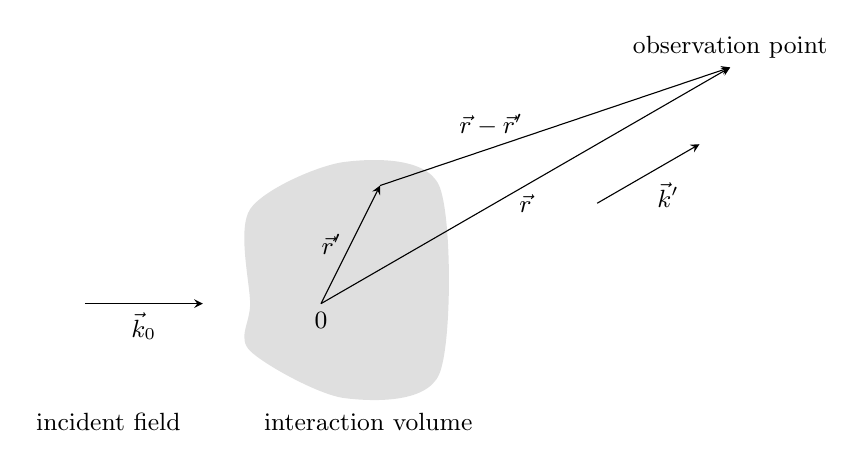
\begin{tikzpicture}[scale=1.5,>=stealth]
    \small
    lightgray = lighten(gray, 0.5);
    \begin{scope}[xshift=0.2cm,scale=0.4]
      \fill[gray!25,%opacity=1
      ] plot [smooth cycle]
      coordinates {(-2,0) (-2,2) (0,3) (2,2.5) (2,-1.5)
        (0,-2) (-2,-1) };
    \end{scope}
    \draw[->] (-2,0)--++(0.5,0)node[below]{$\veck_0$}--+(0.5,0);
    \draw[] (-2.2,0)++(0.4,-1)node[]{incident field};
    \draw[] (0.4,-1)node[]{interaction volume};
    \draw[->] (0,0) -- (30:4)node[above]{observation point};
    \draw[] (30:2)node[below]{$\vecr$};
    \draw[yshift=-0.5cm,->] (30:2.7) 
    --++(30:0.5)node[below right]{$\veck'$} 
    --+(30:0.5);
    \draw[->] (0,0) -- (0.5,1);
    \draw[] (0.25,0.5)node[left]{$\vecr'$};
    \draw[->] (0.5,1) -- (30:4);
    \draw[] (0.5,1) +(20:1)node[above]{$\vecr-\vecr'$};
    \draw[] (0,0)node[below] {$0$};
  \end{tikzpicture}
  \caption[Finite-range scattering potential.]{Finite-range scattering
    potential. A plane wave with wave vector $\veck_0$ is incident on
    the scattering potential which is confined to a small region
    around the origin at $0$. The observation point at $\vecr$ is
    assumed to be far away from the interaction volume.  Points within
    the interaction volume are denoted by $\vecr'$.  The wave vector
    $\veck'$ denotes the propagation direction towards the observer. }
  \label{fig:scattering}
\end{figure}
%%%%%%%%%%%%%%%%%%%%%%%%%%%%%%%%%%%%%%%%%%%%%%%%%%%%%%%%%%%%%%%%%%%%%%
Now let the incident field be a plane wave propagating along
$\veck_0$ with $\abs{\veck_0}=k_0=\omega/c$,
\begin{equation}
  \label{eq:incident-plane-wave}
  \Psi\ho0_\omega(\vecr) = \exp(\ii \veck_0\vecr) \;,
\end{equation}
and the scattering potential be confined to a small region around the
origin as depicted in \cref{fig:scattering}.  If we consider a point
far way from the scattering volume such that
$\abs{\vecr-\vecr'}\approx \abs{\vecr}-\hat{\vecr}\cdot\vecr'$ for
$\abs{\vecr}\gg\abs{\vecr'}$ with the unit vector
$\hat{\vecr}=\frac{\vecr}{\abs{\vecr}}$.  Then the scattered wave
field can be written as
\begin{equation}
  \label{eq:scattered-wave}
  \Psi^{(s)}_\omega(\vecr) = 
  f(\veck',\veck_0)\,\frac{\exp(\ii k_0\abs{\vecr})}{\abs{\vecr}} \;.
\end{equation}
The factor $f$ in front of the outgoing spherical wave is called
scattering amplitude.  Using first-order Born approximation it is
given by
\begin{equation}
  \label{eq:scattering-amplitude}
  f(\veck',\veck_0) = \frac{1}{4\pi}\int\Intddd{\vecr'}
  \exp(-\ii\veck'\vecr')\,V_\omega(\vecr')\,\Psi\ho0_\omega(\vecr') \;,
\end{equation}
where $\veck'=k_0\hat{\vecr}$ denotes the propagation
vector for waves reaching the observation point $\vecr$.  Thus we have
\begin{equation}
  \label{eq:far-field-scattered-wave}
  \Psi_\omega(\vecr) = \exp(\ii \veck_0\vecr) +
  f(\veck',\veck_0)\, \frac{\exp(\ii k_0\abs{\vecr)}}{\abs{\vecr}} \;.
\end{equation}

For the incident plane wave of \cref{eq:incident-plane-wave} and a
point in the far field of the scattering volume, the scattering
amplitude of \cref{eq:scattering-amplitude} evaluated in first-order
Born approximation is given by
\begin{equation}
  \label{eq:scattering-amplitude-first-born}
    f(\veck',\veck_0) 
       = \frac{1}{4\pi}\int\Intddd{\vecr'}
    \exp(-\ii(\veck'-\veck_0)\vecr')V_\omega(\vecr') \;.
\end{equation}
Using the definition of the three-dimensional Fourier transform as in
\cref{eq:ft-k-3}, the scattering amplitude of
\cref{eq:scattering-amplitude-first-born} is identified with the
Fourier transform of the scattering potential as
\begin{equation}
  \label{eq:scattering-amplitude-first-born-ft}
    f(\veck',\veck_0) 
    = \sqrt{\frac{\pi}{2}} \ft{V}_\omega(\veck_0 - \veck') \;.
\end{equation}

To obtain the differential scattering cross-section
$\frac{\difd\sigma}{\difd\Omega}$, let $\vecjin$ denote the number of
incident photons per unit time and unit area and $\vecjsc$ the number
of photon scattered into solid angle $\difd\Omega$ per unit time
traversing an area subtended by $\difd\Omega$.  Then the number of
photons detected within an area $\abs{\vecr}^2\difd\Omega$ at a
distance $\abs{\vecr}$ scattered from an area element $\difd\sigma$
within the scattering volume is given by
\begin{equation}
  \label{eq:scattered-photons}
  \absn{\vecjsc}\abs{\vecr}^2\difd\Omega 
  = \absn{\vecjin}\difd\sigma \;.
\end{equation}
Apart from normalisation factors the current densities are obtained
from $\vecjin\propto\absn{\Psi^{(0)}_\omega}^2$ and
$\vecjsc\propto\absn{\Psi^{(s)}_\omega}^2$.  Using
\cref{eq:far-field-scattered-wave} the differential scattering
cross-section in terms of the scattering amplitude
(\cref{eq:scattering-amplitude}) reads as
\begin{equation}
  \label{eq:differential-scattering-cross-section}
  \frac{\difd\sigma}{\difd\Omega} 
  = \frac{\abs{\vecr}^2\abs{\vecjsc}}{\abs{\vecjin}} 
  = \abs{f(\veck',\veck)}^2 \;.
\end{equation}


\subsubsection{Helmholtz-Kirchhoff integral theorem}
\label{sec:helmholtz-kirchhoff}

%%%%%%%%%%%%%%%%%%%%%%%%%%%%%%%%%%%%%%%%%%%%%%%%%%%%%%%%%%%%%%%%%%%%%%
\begin{figure}
  \centering
  \small
  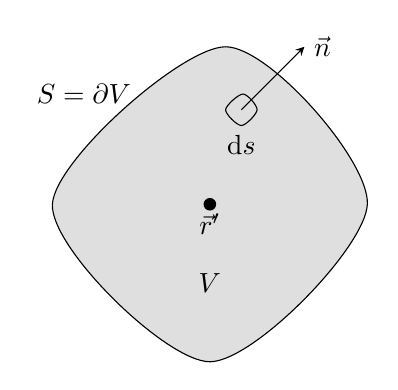
\begin{tikzpicture}[scale=2,>=stealth]
    \fill[gray!25] plot [smooth cycle] 
    coordinates{(-1, 0) (0.1,1) (1,0) (0,-1)};
    \draw[] plot [smooth cycle] 
    coordinates{(-1, 0) (0.1,1) (1,0) (0,-1)};
    \draw (-0.8,0.7)node[]{$S=\pd V$} (0,-0.5)node{$V$};
    \fill[](0,0) circle(0.04) node[below]{$\vecr'$};
    \begin{scope}[xshift=0.2cm,yshift=0.6cm]
      \draw[scale=0.1] plot [smooth cycle] 
      coordinates{(-1, 0) (0.1,1) (1,0) (0,-1)}node[below]{$\difd s$};
      \draw[->] (0,0) -- (0.4,0.4) node[right]{$\vecn$};
    \end{scope}
  \end{tikzpicture}
  \caption[Situation related to the Helmholtz-Kirchhoff diffraction
  integral.]{Situation related to the Helmholtz-Kirchhoff diffraction
    integral.  A volume $V$ is enclosed by a smooth surface $S=\pd V$.
    A point $\vecr'$ within the $V$ is considered to be the (point)
    source of an outgoing spherical wave.  The vector $\vecn$ is
    normal to the surface $S$, and $\difd s$ denotes an infinitesimal
    surface element.  At an arbitrary point $\vecr$ within $V$, the
    value of a wave field governed by the Helmholtz equation is
    determined via the Helmholtz-Kirchhoff diffraction integral, given
    both the field and its first normal derivative over an arbitrary
    surface $S$.}
     \label{fig:kirchhoff}
\end{figure}
%%%%%%%%%%%%%%%%%%%%%%%%%%%%%%%%%%%%%%%%%%%%%%%%%%%%%%%%%%%%%%%%%%%%%%
Let us now consider the situation depicted in \cref{fig:kirchhoff}.
The point $\vecr'$ within the volume $V$ enclosed by the smooth
surface $S=\pd V$ is considered to be the source of an outgoing
spherical wave.  The normal to the surface is denoted by $\vecn$ and
the corresponding surface vector of the infinitesimal surface element
$\difd s$ as $\difd\vecs=\vecn\,\difd s$.  Having an expression of the
Green's function at one's disposal, the Helmholtz-Kirchhoff integral
theorem is derived by means of Green's theorem.  The resulting
diffraction integral expresses the solution of the homogeneous
Helmholtz equation at an arbitrary point $\vecr$ in terms of both the
field and its first normal derivative over an arbitrary smooth and
closed surface enclosing $\vecr$ \cite{PaganinBook,BornWolf} as
\begin{equation}
  \label{eq:helmholtz-kirchhoff}
  \Psi_\omega(\vecr) = \frac{1}{4\pi}\oint_{S}\Intdd{s'}
  \left[G^+_\omega(\vecr-\vecr')\pd_n\Psi_\omega(\vecr') 
    - \Psi_\omega(\vecr')\pd_n G^+_\omega(\vecr-\vecr') \right] \;,
\end{equation}
where $\pd_n$ denotes the derivative normal to the surface $S$ given
by $\pd_n\equiv\vecn\cdot\nabla$.


%%%%%%%%%%%%%%%%%%%%%%%%%%%%%%%%%%%%%%%%%%%%%%%%%%%%%%%%%%%%%%%%%%%%%%
\begin{figure}
  \centering
  \small
  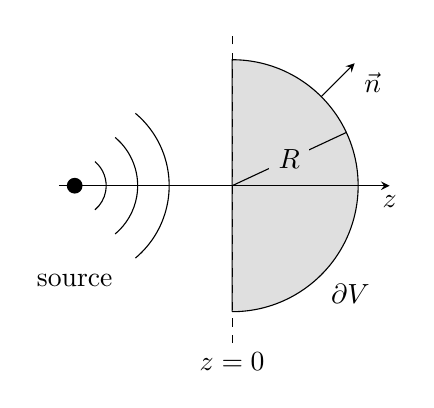
\begin{tikzpicture}[scale=2,>=stealth]
    \def\rr{0.8};
    \filldraw[fill=gray!25] 
    (0,-\rr)--(0,\rr)arc(90:-90:\rr);
    \fill (-1,0)circle (0.05)(-1,-0.5) node[below]{source};
    \foreach \xx in {0.2,0.4,0.6}{
    \draw (-1,0)+(50:\xx) arc(50:-50:\xx);};
    \draw[->] (-1.1,0)--(1,0)node[below]{$z$};
    \draw[dashed](0,-1)node[below]{$z=0$}--(0,1);
    \draw[] (0,0) -- (25:\rr);
    \draw[] (25:\rr/2)node[fill=gray!25]{$R$};
    (0,-\rr)--(0,\rr)arc(90:-90:\rr);
    \draw[](-45:\rr)node[below right]{$\pd V$};
    \draw[->](45:\rr) -- +(45:0.3)node[below right]{$\vecn$};
  \end{tikzpicture}
  \caption[Situation related to a special case of the
  Helmholtz-Kirchhoff diffraction integral.]{Situation related to the
    Helmholtz-Kirchhoff diffraction integral in the case where all
    sources are located within the half\hyph space $z<0$ and emit
    disturbances which propagate along $z$ into the half\hyph space
    $z>0$.  $\vecn$ denotes the outward pointing normal to the surface
    $S=\pd V$.  Supplementing Sommerfeld radiation conditions and
    letting $R\to\infty$, the electromagnetic disturbance at a point
    $\vecr$ within $S$ is determined by the value of both the
    unpropagated wave field and its normal derivative over the plane
    $z=0$. }
     \label{fig:kirchhoff-2}
\end{figure}
%%%%%%%%%%%%%%%%%%%%%%%%%%%%%%%%%%%%%%%%%%%%%%%%%%%%%%%%%%%%%%%%%%%%%%
Let us now consider the case where all sources are located in the
half\hyph space $z<0$ and a wave field propagating along the positive
$z$ direction as depicted in \cref{fig:kirchhoff-2}.  Consider the
surface integration in \cref{eq:helmholtz-kirchhoff} to be performed
over a hemisphere of radius $R$ situated in the half\hyph space
$z>0$ as in \cref{fig:kirchhoff-2}.  To evaluate the
Helmholtz-Kirchhoff diffraction integral for a point $\vecr$ in the
half\hyph space $z>0$ we have to supplement the Sommerfeld radiation
condition, \ie{} we demand that the field and its derivative vanish as
$R\to\infty$.  Then \cref{eq:helmholtz-kirchhoff} transforms into
\begin{equation}
  \label{eq:helmholtz-kirchhoff-plane}
  \begin{split}
      &\Psi_\omega(\vecxp,z>0) =
  \\ &\frac{1}{4\pi}\int_{-\infty}^{\infty}\Intdd{\vecxp'}
  \left(G^+_\omega(\vecr-\vecr')\pd_z\Psi_\omega(\vecr') 
    - \Psi_\omega(\vecr')\pd_z G^+_\omega(\vecr-\vecr') \right)\;,
  \end{split}
\end{equation}
where the $\vecr'$ is confined to the plane $z=0$, thus
$\vecr'=(\vecxp',z'=0)$.


\subsubsection{Rayleigh-Sommerfeld diffraction integral}
\label{sec:Rayleigh-Sommerfeld}

The requirement to know both the field and its derivative over a
closed surface in order to obtain the field at a point within the
surface can be relaxed by an appropriate choice of the Green's
function.  Employing the method of images, a Green's function can be
reconstructed such that either the first or the second term in the
parentheses of \cref{eq:helmholtz-kirchhoff-plane} vanish.  Thus the
remaining integral depends on Neumann or Dirichlet boundary conditions
only.  The Dirichlet Green's function is defined such as to vanish at
the plane $z=0$
\begin{equation}
  \label{eq:dirichlet-greens-function}
  G\ho{D}(\vecr-\vecr') = G^+(\vecr-\vecr') - G^+(\vecr+\vecr') \;.
\end{equation}
The Neumann Green's function is defined such that its derivative
vanishes at $z=0$
\begin{equation}
  \label{eq:neumann-greens-function}
  G\ho{N}(\vecr-\vecr') = G^+(\vecr-\vecr') + G^+(\vecr+\vecr') \;.
\end{equation}
If we consider the same situation as for
\cref{eq:helmholtz-kirchhoff-plane} and use the Dirichlet Green's
function, the Rayleigh-Sommerfeld diffraction integral of the first
kind is obtained as
\begin{equation}
  \label{eq:rayleigh-sommerfeld-1}
  \begin{split}
      \Psi_\omega(\vecr) 
      &= \frac{1}{4\pi}\int_{-\infty}^{\infty}\Intdd{\vecxp'}
      \Psi_\omega(\vecxp',z=0) \pd_z G\ho{D}(\vecr-\vecr')\;.
      \\ &= \frac{1}{2\pi}\int_{-\infty}^{\infty}\Intdd{\vecxp'}
      \Psi_\omega(\vecxp',z=0) 
      \pd_z\frac{\exp(\ii k_0\abs{\vecr-\vecr'})}
      {\abs{\vecr-\vecr'}} \;.
  \end{split}
\end{equation}
Again, $\vecr'$ is confined to the plane $z=0$ and the propagated
field at a point in the half\hyph space $z>0$ is determined by its
boundary value at $z=0$.  In the last line of
\cref{eq:rayleigh-sommerfeld-1} we have used the fact that, due to the
symmetry of the situation, the derivative of the spherical wave
emanating from $-\vecr'$ is the negative of the derivative of the
spherical wave emanating from $\vecr'$.

Employing Neumann boundary conditions, the Rayleigh-Sommerfeld
diffraction integral of the second kind is obtained as
\begin{equation}
  \label{eq:rayleigh-sommerfeld-2}
  \Psi_\omega(\vecr) = -\frac{1}{2\pi}\int_{-\infty}^{\infty}\Intdd{\vecxp'}
   \frac{\exp(\ii k_0 \abs{\vecr-\vecr'})}{\abs{\vecr-\vecr'}}  
   \left.\frac{\pd\Psi_\omega(\vecr')}{\pd z}\right|_{z=0}   \;.
\end{equation}
where, as in \cref{eq:rayleigh-sommerfeld-1}, $\vecr'$ is confined to
the plane $z=0$ and we have invoked the mirror symmetry of the
situation.

\subsection{Fresnel diffraction theory}
\label{sec:fresnel}

Fresnel's formulation of the wave theory of light is a synthesis of
the principle of Huygens and Young \cite{BornWolf}.  According to
Huygens' principle each point on a wave front may be regarded as the
source of secondary waves which combine such that their envelope
determines the wave front at any later point in time
\cite{HuygensYoungFresnel}.  Invoking to this principle Huygens was
able to derive the laws of refraction and reflection.  Conducting his
famous double-slit experiment, Young demonstrated the phenomenon of
interference and enunciated % formulieren, artikulieren
the principle of the interference of light \cite{Young1802}.  By a
combination of Huygens' envelope construction and Young's principle of
interference, Fresnel could explain the rectilinear propagation and
diffraction of light.  Poisson concluded that, according to Fresnel's
theory, a bright spot should appear in the centre of shadow of a small
circular disc blocking a point source of light.  According to Newton's
particle theory of light, which was prevalent at that time, there
should be complete darkness.  Poisson's prediction was experimentally
confirmed by Arago and is since known as Arago spot.

The Fresnel diffraction integral can be derived from the
Rayleigh-Sommerfeld diffraction integral of the first kind
(\cref{eq:rayleigh-sommerfeld-1}) in the paraxial approximation.
First, we will discuss this approximation.  Therefore, we consider the
case of a forward propagating wave front such that its wave vector
$\veck$ subtends a small angle with respect to the optical axis as in
\cref{fig:small-angle-approximation}.
%%%%%%%%%%%%%%%%%%%%%%%%%%%%%%%%%%%%%%%%%%%%%%%%%%%%%%%%%%%%%%%%%%%%%%
\begin{figure}
  \centering
  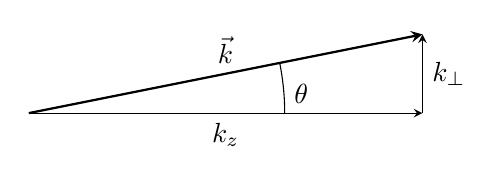
\begin{tikzpicture}[scale=0.5,>=stealth]
  % \clip(-1,-.35)rectangle(1,.35);
  \draw[thick,->] (0,0)->(10,2);
  \node[above] at (5,1) {$\vec{k}$};
  \draw[->] (0,0)->(10,0);
  \node[below] at (5,0) {$k_z$};
  \draw[->] (10,0)->(10,2);
  \node[right] at (10,1) {$k_\perp$};
  \draw[] (6.5,0) arc (0:atan(0.2):6.5cm);
  \node[above right] at (6.5,0) {$\theta$};
  \end{tikzpicture}
  \caption[Small-angle approximation.]{Illustration of the small-angle
    approximation in Fourier space.  The wave vector $\veck$ of the
    incoming light subtends a small angle $\theta$ with respect to the
    optical axis pointing in $z$ direction.}
  \label{fig:small-angle-approximation}
\end{figure}
%%%%%%%%%%%%%%%%%%%%%%%%%%%%%%%%%%%%%%%%%%%%%%%%%%%%%%%%%%%%%%%%%%%%%%
Let $\veckp$ and $k_z$ denote the transverse and the longitudinal
component of the wave vector.  Then the modulus of $\veckp$ and $k_z$
can be approximated as
\begin{equation}
  \label{eq:pa}
  \begin{split}
    k_\perp&\equiv\abs{\veckp}=k\sin\theta\approx k\, \theta \;, \\
    k_z&= k\,\cos\theta \approx k\left(1-\frac{\theta^2}{2}\right) \;.
  \end{split}
\end{equation}
The paraxial approximation refers to the truncation
\begin{equation}
\label{eq:pa-kz}
  k_z\approx k\left(1-\frac{k_\perp^2}{2k^2}\right) \;,
\end{equation}
with $k_\perp\ll k_z$.  \Cref{eq:pa-kz} is also known as slowly varying
envelope approximation, which will become evident in the following.

In the context of the Huygens-Fresnel principle, where wave
propagation is understood as a superposition of forward propagating
spherical waves emanating from point sources, the paraxial
approximation corresponds to the replacement of spherical waves by
parabolic wave fronts in the propagator ($\Prop$) as
\begin{equation}
  \label{eq:spherical-parabolic}
  \exp\left(\ii k \abs{\vecr}\right) =
  \exp\left(\ii k \sqrt{x^2+y^2+z^2}\right) \to
  \exp\left(\ii k z\lrp{1+\frac{x^2+y^2}{2z^2}}\right) \;. 
\end{equation}

Let $a$ denote the size of the smallest length scale that is
resolvable in the wave field and $\lambda$ the wave length of the
probing light, the maximum transverse spatial frequency corresponding
to $a$ is $k_{\perp,\mathrm{max}}=\frac{2\pi}{a}$.  Then the paraxial
approximation amounts to the statement, that the characteristic length
scale $a$ is much larger than the wave length of the probing light:
\begin{equation}
  k_{\perp} \le k_{\perp,\mathrm{max}} = \frac{2\pi}{a} \ll k = 
  \frac{2\pi}{\lambda}
  \quad\Rightarrow\quad a\gg\lambda\;.
\end{equation}
Thus the paraxial approximation is guaranteed to work well above the
diffraction limit which is set by $k=\frac{2\pi}{\lambda}$, see
\cref{sec:angular-spectrum}. % k_{perp,max} ~ k

In the following we derive the Fresnel diffraction integral from
\cref{eq:rayleigh-sommerfeld-1}.  Therefore, we evaluate the
derivative of the Green's function with respect to $z$ as
\begin{equation}
  \label{eq:derivative-propagator}
  \pd_z \frac{\exp(\ii k_0 r)}{r} 
  = \ii k_0\left(1+\frac{\ii}{k_0 r}\right)\frac{z}{r^2}
  \exp\left(\ii k_0 r\right) \;,
\end{equation}
with $r = \abs{\vecr}$.  In the paraxial limit, $r$ appearing the
denominator of \cref{eq:derivative-propagator} can be approximated as
$r\approx z$.  Moreover, in a typical X-ray imaging situation we have
$z = \order(\SI{1}{m})$,
$k_0=\frac{2\pi}{\lambda}=\order(\SI{e10}{m^{-1}})$, and thus
$\frac{1}{k_0 r}\approx 0$.  Oscillations due the exponential in
\cref{eq:derivative-propagator} are small but non-vanishing, and thus
are included to quadratic order in $\vecxp$ as
\begin{equation}
  \label{eq:spherical-parabolic-real}
  r=\abs{\vecr}=z\sqrt{1+\frac{\vecxp^2}{z}} 
  \approx z\left(1+\frac{\vecxp^2}{2z}\right) \;.
\end{equation}
 Hence \cref{eq:derivative-propagator} becomes
\begin{equation}
  \label{eq:fresnel-propagator-limit}
  \pd_z \frac{\exp\left(\ii k_0 r\right)}{r} \to
  \frac{\ii k_0}{z} \exp(\ii k_0 z) 
  \exp\left(\frac{\ii k_0}{2 z} \vecxp^2\right) \;,
\end{equation}
and the formula of the Fresnel diffraction integral is obtained as
\begin{equation}
  \label{eq:fresnel-restored}
  \begin{split}
  &\Psi_\omega(\vecxp,z>0) = 
  \\ & \frac{\ii k_0 \exp(\ii k_0 z)}{2\pi z}
  \int_{-\infty}^{\infty}\Intdd{\vecxp'}
  \Psi_\omega(\vecxp',z=0) 
  \expp{\frac{\ii k_0}{2 z}(\vecxp-\vecxp')^2} \;.
  \end{split}
\end{equation}
\Cref{eq:fresnel-restored} corresponds to the integral form of the
paraxial wave equation supplemented by boundary conditions, which will
be derived in the following.

Recall the homogeneous Helmholtz equation for the monochromatic
component of a complex scalar field
\begin{equation}
  \label{eq:helmholtz-2}
  \left(\nabla^2 + k^2\right)\Psi_\omega(\vecr)=0\;,
\end{equation}
with wave number $k=n\frac{\omega}{c}$ and $n=\const$.  In the
paraxial limit the Helmholtz equation reduces to the paraxial wave
equation as follows.  Consider an ansatz for the wave field in the
form of a plane wave propagating along the optical axis with wave
vector $k_z$ and modulated by the envelope $\Psi\env_{\omega}$ as
\begin{equation}
  \label{eq:ansatz-env}
  \Psi_{\omega}(\vecr)=\Psi\env_{\omega}(\vecr)\,\exp(\ii k z)\;.
\end{equation}
Inserting ansatz \eqref{eq:ansatz-env} into \cref{eq:helmholtz-2}, we
obtain a partial differential equation for the envelope function as
\begin{equation}
  \label{eq:ansatz-env-in-helm}
  \begin{split}
    0&=\left(\nabla^2 +2\ii k\pd_z\right)\Psi\env_{\omega}(\vecr)\\
    &=\left(\nabla_\perp^2+2\ii k\pd_z+\pd_z^2\right)
    \Psi\env_{\omega}(\vecr)\;,
  \end{split}
\end{equation}
where we have decomposed the Laplace operator into a transverse
($\nabla_\perp^2$) and a longitudinal part ($\pd_z^2$).  If the
transverse variations of $\Psi_\omega\env$ exceed the longitudinal
ones, the second derivative $\pd_z^2\Psi_{\omega}\env$ may be omitted
in \cref{eq:ansatz-env-in-helm}.  Such a wave front is called
beam-like.  The resulting parabolic partial differential equation is
referred to as homogeneous paraxial wave equation:
\begin{equation}
  \label{eq:pwe}
  \left(\nabla_\perp^2 +2\ii k\pd_z\right)\Psi\env_{\omega}(\vecr) = 0 \;.
\end{equation}
This is a Schrödinger equation for the z-evolution of the wave field
$\Psi\env_{\omega}$, \ie{} quantum mechanics in two spatial ($\vecxp$)
and one temporal ($z$) dimensions \cite{Schroedinger1926}.  Along the
lines of the conservation of probability of a wave function governed
by Schrödinger's equation, the conservation of intensity can be
derived from \cref{eq:pwe}.  For the intensity of the wave field
$\Psi_\omega$ we have
\begin{equation}
  \label{eq:intensity-fresnel}
  I_\omega = \abs{\Psi_\omega}^2 = \absn{\Psi\env_\omega}^2 \;.
\end{equation}
In analogy to the probability current in non-relativistic quantum
mechanics, we define the flux of intensity which is transverse to the
direction of propagation as
\begin{equation}
  \label{eq:fresnel-current}
  \begin{split}
      \vecj_\omega 
      & =  \frac{1}{2\ii k}\lrb{ \lrp{ 
          \Psi_\omega\env}^* \np \Psi_\omega\env 
        - \Psi_\omega\env \np \lrp{\Psi_\omega\env}^* }
      \\ & =  \frac{1}{2\ii k}\lrb{ \lrp{ 
          \Psi_\omega}^* \np \Psi_\omega 
        - \Psi_\omega \np \lrp{\Psi_\omega}^* }
      \\ & = \frac{1}{k} I_\omega\np\phi_\omega \;.
  \end{split}
\end{equation}
In the last line of \cref{eq:fresnel-current} we have expressed the
wave field in terms of  phase and amplitude as
\begin{equation}
  \label{eq:amplitude-phase}
  \Psi_\omega(\vecr)=\sqrt{I_\omega(\vecr)}\expp{\ii\phi_\omega(\vecr)} \;.
\end{equation}
Using the above definitions a continuity equation for Fresnel theory
follows as
\begin{equation}
  \label{eq:continuity-fresnel}
  \pd_z I_\omega + \np\cdot\vecj_\omega = 0 \;.
\end{equation}
Thus, the conservation of probability for the time evolution of a wave
function governed by Schrödinger's equation in quantum mechanics
translates into the conservation of intensity for a forward
propagating paraxial wave field in Fresnel theory.  This is just the
conservation of energy under forward propagation.  Defining the
'power' $P$ that is irradiated along the optical axis from a source
located upstream into the \acf{fov} as
\begin{equation}
  \label{eq:power}
  P = \int_\fov\Intdd{\vecxp} I_\omega \;,
\end{equation}
the integral version of \cref{eq:continuity-fresnel}  reads
\begin{equation}
  \label{eq:continuity-fresnel-integral}
  \frac{\difd P}{\difd z} 
  + \oint_{\pd\fov}\Intdd{\vec{s}}\vecj_\omega = 0 \;,
\end{equation}
where $d\vec{s}$ denotes the vector 'surface' element normal to the
boundary $\pd\fov$.

We now show that the Fresnel diffraction integral is the integral form
of the paraxial wave equation, supported by Dirichlet boundary
conditions at $z=0$.  Using the Fourier transform as defined in
\cref{eq:ft-k-2}, the Fourier representation of $\Psi\env_{\omega}$
reads
\begin{equation}
  \label{eq:ift-psi-env}
  \Psi\env_{\omega}(\vecxp)  = \iF_{\vecxp} \ft{\Psi}\env_{\omega} = 
  \frac{1}{2\pi}\int_{-\infty}^\infty \Intdd{\veckp} 
  \ft{\Psi}\env_{\omega}(\veckp) \exp(-\ii\veckp\vecxp) \;.
\end{equation}
Inserting \cref{eq:ift-psi-env} into the paraxial wave equations, we
obtain the following equation for the Fourier components
$\ft{\Psi}\env_{\omega}$
\begin{equation}
  \label{eq:pwe-fourier}
  \left( -\veckp^2  +2\ii k\pd_z \right)
  \ft{\Psi}\env_{\omega}(\veckp,z) = 0\;. 
\end{equation}
Assuming $\veckp$ to be fixed, \cref{eq:pwe-fourier} converts into an
ordinary differential equation for $\ft{\Psi}\env_\omega$ in $z$ which
can be solved upon a separation of variables as
\begin{equation}
  \label{eq:envelop-ode}
  \frac{\difd\ft{\Psi}\env_\omega}{\ft{\Psi}\env_\omega} 
  = \frac{-\ii \veckp^2}{2 k} \difd z \;.
\end{equation}
Integration of \cref{eq:envelop-ode} yields the Fourier transform of
the envelope wave field as
\begin{equation}
  \label{eq:envelope-fourier}
  \ft{\Psi}\env_\omega(\veckp,z>0) 
  = \ft{\Psi}\env_\omega(\veckp,0)\exp(-\frac{\ii z}{2 k}\veckp^2) \;.
\end{equation}
Substitution of \cref{eq:envelope-fourier} into the Fourier
representation of $\ft{\Psi}\env_\omega$ yields an integral solution
for $\Psi\env_{\omega}$.  Resubstituting $\Psi_{\omega}\env=
\Psi_{\omega}\exp(-\ii k z)$, we obtain the Fresnel diffraction
integral for the forward propagating wave field $\Psi_{\omega}$ as
\cite{PaganinBook,BornWolf}
\begin{equation}
  \label{eq:fresnel}
  \Psi_{\omega}(\vecxp,z>0) = \e{\ii k z}\F^{-1}
  \left[\expp{-\frac{\ii z}{2k}\veckp^2}\;
    \F[\Psi_{\omega}(\vecxp,z=0)]\right]\;,
\end{equation}
given its boundary values at $z=0$

A real-space version of \cref{eq:fresnel} is found by appeal to the
convolution theorem of \cref{eq:convolution-theorem-k-n}.  Let $\conv$
denote the two-dimensional convolution with respect to the transverse
coordinates $\vecxp$ as in \cref{eq:convolution-n}, the convolution
theorem in two dimension for the Fourier transform as defined in
\cref{eq:ft-k-2} reads
\begin{equation}
  \label{eq:convolution-theorem-k-2}
  \F[f \conv g] = 2\pi (\F f) \times (\F g) \;.
\end{equation}
By means of \cref{eq:convolution-theorem-k-2} the Fourier transform
formulation of the \cref{eq:fresnel} is recast into a convolution
integral as
\begin{equation}
  \label{eq:fresnel-conv}
  \begin{split}
      \Psi_{\omega}(\vecxp,z>0) 
       &= \int\Intdd{\vecxp'}
       \Prop_F(\vecxp-\vecxp',z)\,\Psi_{\omega}(\vecxp',z=0)
    \\ &= \Prop_F(\vecxp,z)\conv\Psi_{\omega}(\vecxp,z=0)\;.
  \end{split}
\end{equation}
The function $\Prop_F$ is called  Fresnel propagator.  Comparing
\cref{eq:fresnel,eq:fresnel-conv} the Fresnel propagator in Fourier
space reads 
\begin{equation}
  \label{eq:fresnel-propagator-fourier}
  (\F\Prop_F)(\veckp,z) = 
  \frac{\exp(\ii k z)}{2\pi}\exp\left(-\frac{\ii z}{2k}\veckp^2\right) \;.
\end{equation}
The real-space version of $\Prop_F$ is obtained from the inverse
Fourier transformation of \cref{eq:fresnel-propagator-fourier}.  The
Fourier integral is evaluated upon quadratic completion and use of the
Gaussian integral formula.  It is given by
\begin{equation}
  \label{eq:fresnel-propagator}
  \Prop_F(\vecxp,z) = 
  \frac{-\ii k}{2\pi z} \exp(\ii k z) 
  \exp\left(\frac{\ii k}{2z}\vecxp^2\right) \;.
\end{equation}

Given a monochromatic wave front at $z=0$, the intensity at distance
$z$ computes as
\begin{equation}
  \label{eq:intensity-scalar}
  I_\omega(\vecxp,z>0) = \abs{\Psi_{\omega}(\vecxp,z>0)}^2 \;.
\end{equation}
\Cref{eq:fresnel} is well apt for a numerical implementation by means
of \ac{fft} algorithms in order to simulate the intensity map for a
given wave field $\Psi_{\omega}(\vecxp,z=0)$.

Let us express the wave field at the boundary $z=0$ in terms of a
(frequency-dependent) amplitude and phase as
\begin{equation}
  \label{eq:exit-wave}
  \Psi_{\omega}(\vecxp,z=0) = 
  \expb{-B_\omega(\vecxp)}\expb{\ii\phi_\omega(\vecxp)} \;.
\end{equation}
The intensity obtained from the Fresnel diffraction integral is
invariant under a global shift of the phase
\begin{equation}
  \label{eq:global-phase-shift}
  \phi_\omega(\vecxp) \to \phi_\omega'(\vecxp) =  
  \phi_\omega(\vecxp) +  \bar{\phi}_\omega \;,
\end{equation}
with $\bar{\phi}_\omega=\const$.  However, a global shift
$\bar{B}_\omega$ of the attenuation
\begin{equation}
  \label{eq:global-attenuation-shift}
  B_\omega(\vecxp) \to B_\omega'(\vecxp) = 
  B_\omega(\vecxp) + \bar{B}_\omega 
\end{equation}
entails a rescaling of the intensity.  Namely, under global shifts of
phase and attenuation, the Fresnel diffraction integral implies that
\begin{equation}
  \label{eq:intensity-rescaling}
  I_\omega(\phi_\omega,B_\omega) \to I_\omega'(\phi_\omega',B_\omega') = 
  \exp(-2\bar{B}_\omega)I_\omega(\phi_\omega,B_\omega) \;.
\end{equation}
Thus a phase retrieved in Fresnel theory is only defined modulo a
constant offset.


\subsubsection{Fraunhofer diffraction}
\label{sec:fraunhofer}

Fraunhofer diffraction refers to Fresnel diffraction in the case of
propagation distances that are large compared to the characteristic
scale of the unpropagated wave field.  The expression for Fraunhofer
diffraction is found upon expanding the exponential in the integrand
of \cref{eq:fresnel-restored}.  The disturbance to be propagated from
the plane $z=0$ is considered to be non-negligible only over a region
of diameter $a$.  If the Fresnel number $N_F$ is much less than
unity,
\begin{equation}
  \label{eq:fresnel-number}
  N_F\equiv \frac{a^2}{\lambda z} \ll 1 \;,
\end{equation}
we may ignore the term quadratic in $\vecxp'^2\le a^2$ in the exponent
of \cref{eq:fresnel-restored}.  The Fraunhofer diffraction integral
then follows from the Fresnel diffraction integral as
\begin{equation}
  \label{eq:fraunhofer}
  \begin{split}
  \Psi_\omega(\vecxp&,z>0) =
   \frac{\ii}{\lambda_0 z}\exp(\ii k_0 z)
  \expp{\frac{\ii k_0}{2 z} \vecxp^2}
  \\ &\times\int_{-\infty}^{\infty}\Intdd{\vecxp'}\Psi_\omega(\vecxp',z=0) 
  \expp{-\frac{\ii k_0}{z}\vecxp\cdot\vecxp'} \;.    
  \end{split}
\end{equation}
The intensity pattern arising from Fraunhofer diffraction is thus
given by the (rescaled) Fourier transform of the boundary wave field
evaluated at frequencies $\veckp=\frac{k_0}{z}\vecxp$.

Next we consider the Fraunhofer diffraction pattern emerging from a
circular aperture of radius $a$.  Introducing polar coordinates
\begin{equation}
  \label{eq:polar-2}
  \vecxp = \vv{x}{y} = 
  \vv{r \cos\theta}{r \sin\theta} \;,
\end{equation}
the diffraction integral \cref{eq:fraunhofer} for a circular aperture
reads
\begin{equation}
  \label{eq:fraunhofer-circular}
  \begin{split}
  \Psi_\omega(\vecxp,&z>0) =
   \frac{\ii }{\lambda_0 z}\exp(\ii k_0 z)
  \expp{\frac{\ii k_0}{2 z} \vecxp^2}
  \\ &\times\int_0^a\Intd{r'}\int_0^{2\pi}\Intd{\theta'} r 
  \expp{-\frac{\ii k_0}{z}r\,r' \cos(\theta-\theta')} \;.    
  \end{split}
\end{equation}
The angular integration in \cref{eq:fraunhofer-circular} is identified
with an integral representation of the Bessel function of first kind
and zeroth order $J_0$ \cite{BornWolf}.  We thus have
\begin{equation}
  \label{eq:fraunhofer-circular-bessel}
  \begin{split}
    \Psi_\omega(\vecxp,&z>0) =
    \frac{\ii 2 \pi}{\lambda_0 z}\exp(\ii k_0 z)
    \expp{\frac{\ii k_0}{2 z} \vecxp^2}
    \\ & \times\int_0^a\Intd{r'} r'\, J_0\lrp{\frac{k_0 r\,r'}{z}} \;.
  \end{split}
\end{equation}
Using a recurrence relation between $J_0$ and the Bessel function of
first kind and first order $J_1$ \cite{BornWolf},
\cref{eq:fraunhofer-circular-bessel} becomes
\begin{equation}
  \label{eq:fraunhofer-circular-bessel-2}
  \Psi_\omega(\vecxp,z>0) = 
  \frac{\ii\pi a^2}{\lambda_0 z}\exp(\ii k_0 z)
  \expp{\frac{\ii k_0}{2 z} \vecxp^2}
  \frac{2 J_1\lrp{\frac{k_0 r a}{z}} }{\frac{k_0 r a}{z}} \;.
\end{equation}
This is a well-know formula first derived by Airy.  The diffraction
pattern resulting from \cref{eq:fraunhofer-circular-bessel-2} is thus
called Airy pattern \cite{Airy1835}, see \cref{fig:airy}.
%%%%%%%%%%%%%%%%%%%%%%%%%%%%%%%%%%%%%%%%%%%%%%%%%%%%%%%%%%%%%%%%%%%%%%
\begin{figure} 
  % Plot created with mathematica
  \centering
  \psfragfig[%width=0.5\textwidth,
  height=0.25\textheight]
  {figures/Airy/AiryFunction}{
    \small
    \psfrag{x}[c][c]{$x$}
    \psfrag{y}[c][c]{$I_z(x)/I_0$}
    \psfrag{1.0}{1.0} 
    \psfrag{-10}{-10} \psfrag{-5}{-5}
    \psfrag{0}{0} \psfrag{5}{5} \psfrag{10}{10} 
    % \psfrag{0.2}{0.2} \psfrag{0.4}{0.4} \psfrag{0.6}{0.6}
    % \psfrag{0.8}{0.8} 
    \psfrag{1}{1} \psfrag{2}{2} \psfrag{4}{4}\psfrag{6}{6}
    \psfrag{8}{8} 
  }
  \caption[Fraunhofer diffraction at a circular aperture (Airy
  pattern).]{Airy pattern emerging from Fraunhofer diffraction at a
    circular aperture of radius $a$.  The normalised intensity is
    given by $\frac{I_z(x)}{I_0}=\lrb{2\frac{J_1(x)}{x}}^2$ where
    $J_1$ denotes the Bessel function of the first kind and first
    order.  The abscissa is $x=\frac{k_0 r a}{z}$ with wave vector
    $k_0\equiv\frac{2\pi}{\lambda_0}$ and $r$ being the distance to
    the optical axis in the observation plane.  First and second
    minima occur at $x=\num{3.833}$ and 7.016, respectively.}
  \label{fig:airy}
\end{figure}
%%%%%%%%%%%%%%%%%%%%%%%%%%%%%%%%%%%%%%%%%%%%%%%%%%%%%%%%%%%%%%%%%%%%%%



\subsubsection{Angular spectrum representation}
\label{sec:angular-spectrum}

In the following we consider the angular spectrum approach to
construct a solution to the Helmholtz equation for a forward
propagating field in terms of plane waves.  It will become evident
from the angular spectrum approach that plane waves with the
transverse wave vector components exceeding the modulus of the wave
vector $k$ correspond to evanescent waves; the amplitude of which
decay exponentially with propagation distance.  Thus transverse length
scales related to transverse components of the wave vector cannot be
resolved in the far field, which is a statement of the diffraction
limit.

Consider a plane wave denoted as
\begin{equation}
  \label{eq:plane-wave-ansatz}
  \Psi_\omega\hon{p w}(\vecr)=\exp(\ii \veck\vecr) \;,
\end{equation}
with $\vecr=(\vecxp,z)$ and wave vector $\veck=(\veckp,k_z)$.
Inserting ansatz \cref{eq:plane-wave-ansatz} into the Helmholtz
equation \eqref{eq:helmholtz-2} fixes the modulus of the wave vector
to $\abs{\veck}=k=\frac{\omega}{c}$, which we solve for $k_z$.  Taking
the positive solution of $k_z$, which corresponds to propagation along
the positive $z$\hyph direction, the plane wave solution reads
\begin{equation}
  \label{eq:plane-wave-kz}
  \begin{split}
    \Psi_\omega\hon{p w}(\vecxp,z) 
    & = \exp(\ii\veckp\vecxp)\expp{\ii\sqrt{k^2-\vecxp^2}z}
    \\ & = \Psi_\omega\hon{p w}(\vecxp,z=0) \expp{\ii\sqrt{k^2-\vecxp^2}z} \;.
  \end{split}
\end{equation}
We assume an arbitrary wave field to be given at the plane $z=0$.  Its
(transverse) Fourier representation reads
\begin{equation}
  \label{eq:boundary-wave-field}
  \Psi_\omega(\vecxp,z=0) 
  = \frac{1}{2\pi}\int\Intdd{\veckp}\ft{\Psi}_\omega(\veckp,z=0)
  \expp{\ii\veckp\vecxp} \;.
\end{equation}
Since \cref{eq:plane-wave-kz} represents a plane wave propagated from
$z=0$ to distances $z>0$ and \cref{eq:boundary-wave-field} the
boundary wave field decomposed it into plane waves, the wave field of
\cref{eq:boundary-wave-field} propagated to distances $z>0$ can be
composed as
\begin{equation}
  \label{eq:plane-wave-solution}
  \begin{split}
      \Psi_\omega&(\vecxp,z>0) 
 \\ & =  \frac{1}{2\pi} \int\Intdd{\veckp}
  \ft{\Psi}_\omega(\veckp,z=0)\expp{\ii\veckp\vecxp}\expp{\ii k_z z} \;,
  \end{split}
\end{equation}
with $k_z =\sqrt{k^2-\veckp^2}$. 

For plane waves with $\veckp>k$, the longitudinal component $k_z$
becomes imaginary and the according exponent in
\cref{eq:plane-wave-solution} real.  Thus, plane waves with
$\abs{\veckp}>k$ decay exponentially.  After $\Psi_\omega$ has
propagated from $z=0$ to the far field, only plane waves with
$\veckp<k$ will remain to contribute to the diffraction pattern.  The
maximum of the transverse wave vector $k_{\perp,\mathrm{max}}$ relates
to the smallest resolvable transverse length scale $\Delta x$ within
the unpropagated wave field as
\begin{equation}
  \label{eq:diffraction-limit}
  k_{\perp,\mathrm{max}}\equiv\frac{2\pi}{\Delta x} 
  \le\frac{2\pi}{\lambda} \;.
\end{equation}
This is a statement of the diffraction limit.

\subsection{Projection approximation}
\label{sec:proj-approx}


%%%%%%%%%%%%%%%%%%%%%%%%%%%%%%%%%%%%%%%%%%%%%%%%%%%%%%%%%%%%%%%%%%%%%%
\begin{figure}
  \centering
  \small
  \def\yy{0.8}
  \def\radius{0.8}
  \begin{tikzpicture}[scale=2,>=stealth,domain=-\yy:\yy]
  \def\yy{0.8};
  \def\radius{0.8};
    % incident wave front
    \foreach \y in {-0.7,-0.5,...,0.7}{
      \draw[thick,->] (0,\y) -> (1,\y);}
    \draw[thick] (1.2,-1) -- (1.2,1)node[above]{plane wave crest};
    \draw[] (0.5,-1) node[below]{incident wave};
    % sample
    \filldraw[color=gray!25] ({1.4+\radius},0) circle(\radius);
    \node[below] at (2.2,-1) {sample $n_\omega$};
    % incident intensity
    \draw[dashed, help lines] (1.4,1)--(1.4,-1) node[below,black]{$\Iin$};
    \draw[dashed, help lines] (3,1)--(3,-1) node[below,black]{$I_{z_0}$};
    % z axis
    \draw[->] (0,0) -> (4.4,0)node[below] {$z$};
    \draw[] (1.4,-0.1) node[below left] {$0$} -- (1.4,0.1);
    \draw[] (3,-0.1)node[below left] {$z_0$} -- (3,0.1);
    % exit wave front
    \begin{scope}[thick,xshift=2.25cm]
      \draw[] plot ({cos(\x^2 r)},\x);
      \draw[]({cos(\yy^2 r)},\yy)--({cos(\yy^2 r)},1);
      \draw[]({cos(\yy^2 r)},1.05) node[above]{exit wave crest};
      \draw[]({cos(\yy^2 r)},-\yy)--({cos(\yy^2 r)},-1);
    \end{scope}
    % diffraction
    \foreach \y in {-0.7,-0.5,-0.3,-0.1,0.1,0.3,0.5,0.7}{
      \draw[thick,->] (3.3,\y) --++ 
      ({2/sqrt(2+(\y/sqrt((0.8)^2-(\y)^2) )^2)/1.4},
 {(\y/sqrt((0.8)^2-(\y)^2) )/sqrt(2+(\y/sqrt((0.8)^2-(\y)^2) )^2)/1.4});}
  \draw (3.8,-1) node[fill=white!100,below,align=center]
  {diffraction};
  \end{tikzpicture}
  \caption[Projection approximation and forward propagating in Fresnel
  theory.]{Projection approximation and forward propagating in Fresnel
    theory. An incident monochromatic plane wave of constant intensity
    $\Iin$ impinges on the sample at $z=0$ and exits at $z=z_0$ with
    intensity $I_{z_0}\equiv I_\omega(\vecxp,z_0)$.  The interaction
    of light with matter is described in terms of the refractive index
    $n_\omega$.  While traversing the sample the incident wave
    accumulates phase shift and attenuation according to
    \cref{eq:phase-shift,eq:attenuation}, causing local diffraction at
    the object exit.  Subsequent self-interference upon forward
    propagation of the diffracted exit wave front is described by the
    Fresnel diffraction integral, see \cref{sec:fresnel}.}
  \label{fig:forward-propagation}
\end{figure}
%%%%%%%%%%%%%%%%%%%%%%%%%%%%%%%%%%%%%%%%%%%%%%%%%%%%%%%%%%%%%%%%%%%%%%
Consider the situation of an imaging experiment as depicted in
\cref{fig:forward-propagation}.  Here a monochromatic plane wave
propagates along the optical axis $z$ and is incident upon a sample
which is described in terms of an inhomogeneous refractive index
$n(\vecr)$.  This situation is governed by the inhomogeneous Helmholtz
equation \eqref{eq:helmholtz-inhomo}.  Assuming paraxiality of the
traversing wave field as discussed in \cref{sec:fresnel},
\cref{eq:helmholtz-inhomo} transforms into the inhomogeneous paraxial
wave equation for the envelope wave field $\Psi\env_{\omega}$,
\begin{equation}
    \label{eq:pwe-inhom}
    \left(\nabla_\perp^2 + 2\ii k\pd_z + k^2[n_\omega^2(\vecr)-1]\right) 
    \Psi\env_{\omega}(\vecr)=0\;.
\end{equation}
In the X-ray regime the refractive index is typically close to unity
and its real part smaller than one.  Thus a dense region in the sample
would cause the phase of the incident wave field to advance relative
to its surroundings.  It is convenient to express the refractive index
in terms of a real part decrement $\delta_\omega$ and an imaginary
part $\beta_\omega$ as
\begin{equation}
  \label{eq:n-xray}
  n(\omega) = 1 -\delta_\omega +\ii\beta_\omega\;,
\end{equation}
where $\delta_\omega$ and $\beta_\omega$ are small real numbers and
depend on the frequency $\omega$.  While the real-part decrement
$\delta_\omega$ is attributed to elastic scattering, the imaginary
part $\beta_\omega$ is related to the attenuation of the electromagnetic
wave in an absorptive medium, see
\cref{sec:scattering,sec:absorption}, respectively.  Below the
threshold for the creation of an electron\hyph positron pair, the
refractive index approaches unity with increasing energy and 
$\delta_\omega$ and $\beta_\omega$ tend to zero, see
\cref{fig:refractive-index} and \cref{sec:interaction}.  In the X-ray
regime and away from absorption edges, see \cref{sec:absorption}, the
refractive index decrement is typically several orders of magnitude
larger than the imaginary part.
%%%%%%%%%%%%%%%%%%%%%%%%%%%%%%%%%%%%%%%%%%%%%%%%%%%%%%%%%%%%%%%%%%%%%%
\begin{figure}
  \centering
    \psfragfig[width=.8\textwidth,height=0.55\textwidth]
    {figures/RefractiveIndex/fig_delta}
    { \small
      \psfrag{Energy}[c][c]{Energy $E$ [\si{eV}]}
      \psfrag{delta}[c][r]{Real part decrement $\delta_\omega$}
      \psfrag{iron}{Iron}\psfrag{calcium}{Calcium}
      \psfrag{silicon}{Silicon}\psfrag{carbon}{Carbon}
      \psfrag{waterwater}{Water}
    } \\ \vspace{-0.05cm}
    \psfragfig[width=.8\textwidth,height=0.55\textwidth]
    {figures/RefractiveIndex/fig_beta}
    { \small
      \psfrag{Energy}[c][c]{Energy $E$ [\si{eV}]}
      \psfrag{beta}[c][r]{Imaginary part $\beta_\omega$}
      \psfrag{iron}{Iron}\psfrag{calcium}{Calcium}
      \psfrag{silicon}{Silicon}\psfrag{carbon}{Carbon}
      \psfrag{waterwater}{Water}
    } \\ \vspace{-0.05cm}
    \psfragfig[width=.8\textwidth,height=0.55\textwidth]
    {figures/RefractiveIndex/fig_ratio}
    { \small
      \psfrag{Energy}[c][c]{Energy $E$ [\si{eV}]}
      \psfrag{ratio}[c][r]{Ratio $\delta_\omega / \beta_\omega$}
      \psfrag{iron}{Iron}\psfrag{calcium}{Calcium}
      \psfrag{silicon}{Silicon}\psfrag{carbon}{Carbon}
      \psfrag{waterwater}{Water}
    }
      % \psfrag{10}{10}\psfrag{2}{2}\psfrag{3}{3}\psfrag{4}{4}
      % \psfrag{0}{0}\psfrag{-2}{-2}\psfrag{-3}{-3}
      % \psfrag{-4}{-4}\psfrag{-6}{-6}\psfrag{-8}{-8}\psfrag{-10}{-10}
    \caption[The refractive index in dependence of energy.]{The
      refractive index $n(\omega)=1-\delta_\omega +\ii\beta_\omega$
      and the ratio $\frac{\delta_\omega}{\beta_\omega}$ as a function
      of photon energy $E=\hbar\omega$ for various substances at room
      temperature.  Apart from the regions close to absorption edges,
      both $\delta_\omega$ and $\beta_\omega$ decrease with increasing
      energy and the refractive index approaches unity.  The ratio
      $\frac{\delta_\omega}{\beta_\omega}$, however, increases with
      energy.}
  \label{fig:refractive-index}
\end{figure}
%%%%%%%%%%%%%%%%%%%%%%%%%%%%%%%%%%%%%%%%%%%%%%%%%%%%%%%%%%%%%%%%%%%%%%

The projection approximation amounts to a neglect of the transverse
Laplacian in \cref{eq:pwe-inhom} which couples neighbouring ray
trajectories.  Thus, using the small-angle approximation,
\cref{eq:n-xray}, and disregarding scattering away from the ray path,
the inhomogeneous paraxial wave equation \eqref{eq:pwe-inhom} reduces
to
\begin{equation}
    \label{eq:proj-approx-0}
    \pd_z\Psi\env_{\omega}(\vecr) = 
    -k_0\left[\ii  \delta_\omega(\vecr) +\beta_\omega(\vecr)\right]
    \Psi\env_{\omega}(\vecr)\;,
\end{equation}
A solution to this boundary value problem is given by
\begin{equation}
  \label{eq:transmission-0}
    \Psi\env_{\omega}(\vecxp,z) = 
    \exp\left(\ii\phi_\omega(\vecxp,z_0) -B(\vecxp,z_0) \right) 
    \Psi\env_{\omega}(\vecxp,z=0) \;,
\end{equation}
where we have introduced phase shift and attenuation of the exit
wave front as
\begin{equation}
  \label{eq:phase-shift}
  \phi_\omega(\vecxp,z_0) = 
  -k_0\int_{z=0}^{z=z_0}\Intd{z}\delta_\omega(\vecxp,z) \;,
\end{equation}
and
\begin{equation}
  \label{eq:attenuation}
  B_\omega(\vecxp,z_0) = 
  k_0\int_{z=0}^{z=z_0}\Intd{z}\beta_\omega(\vecxp,z) \;,
\end{equation}
respectively.  Introducing the transmission function as
\begin{equation}
  \label{eq:transmission-function}
  T_\omega (\vecxp) 
  \equiv \expp{\ii\phi_\omega(\vecxp,z_0)-B_\omega(\vecxp,z_0)} \;,
\end{equation}
we may write the wave field immediately downstream the object as
\begin{equation}
  \label{eq:transmission}
  \Psi\env_\omega(\vecxp,z_0) \equiv 
  T_\omega(\vecxp)\Psi_\omega\hon{in}(\vecxp) \;,
\end{equation}
where $\Psi_\omega\hon{in}(\vecxp) \equiv
\Psi\env_{\omega}(\vecxp,z=0)$ denotes the incident wave field.  The
functions $\phi_\omega$ and $B_\omega$ essentially are Radon
transforms of the refractive index along the ray path
\cite{Radon1917}, see \cref{eq:projection-radon}, and can be
interpreted as the projection of the electron density as will be shown
in \cref{sec:scattering,sec:absorption}.  If $\beta_\omega$ is assumed
to be constant, we may define the linear attenuation coefficient
$\mu_\omega$ as
\begin{equation}
  \label{eq:linear-attenuation}
  \mu_\omega = \frac{2}{z_0}B_\omega=2k_0\beta_\omega \;.
\end{equation}
From \cref{eq:transmission-0} and using $I_\omega = \abs{\Psi_\omega}^2$
we obtain Beer's law of absorption
\begin{equation}
  \label{eq:beers-law}
  I_\omega(\vecxp,z) = I_\omega(\vecxp,z=0)\exp(-\mu_\omega z)
\end{equation}
for $z<z_0$.


\subsection{Filtered backprojection}
\label{sec:fbp}

%%%%%%%%%%%%%%%%%%%%%%%%%%%%%%%%%%%%%%%%%%%%%%%%%%%%%%%%%%%%%%%%%%%%%%
\begin{figure}
  \centering
  \begin{tikzpicture}[scale=1.5,>=stealth]
    \small
    \def\rotangle{38};
    \def\cortop{2cm};
    \def\corlow{1.6cm};
    \def\fcorw{1.3cm};
    % REAL SPACE 
     \node[rotate=\rotangle,inner sep=0pt] (shepplogan) at (0,0)
     {\includegraphics[width=3cm]{figures/FourierSliceTheorem/Phantom.png}};
    \draw[->](-\cortop,0) -- (\cortop,0) node[below] {$x$};
    \draw[->](0,-\corlow)--(0,\cortop)node[left] {$y$};
    % FOURIER SPACE
    \begin{scope}[xshift={\cortop+\fcorw+0.8cm}]
%      \filldraw[blue!20!white!80](0,0) circle(1);
       \node[inner sep=0pt] (shepploganft) at (0,0)
  {\includegraphics[width=3cm]{figures/FourierSliceTheorem/Phantom_FT.png}};
      \draw (-0.9,-0.9) node[] {$\F f$};
%      \shade plot [smooth cycle] coordinates{(-1, 0) (0,1) (1,0) (0,-1)}
      \draw[->](-\fcorw,0)--(\fcorw,0) node[below] {$\xi_x$};
      \draw[->](0,-\corlow)--(0,\cortop)node[left] {$\xi_y$};
%      \draw[->] (0,0) -- (\rotangle+90:1) node[right]{$\vecxi$};
      \draw[](\rotangle-90:1.6)--(\rotangle+90:1.6)node[above]
      {$\left.(\F f)\right|_{\theta=\Theta+\frac{\pi}{2}}$};
      \draw[] (0.8,0)arc(0:{\rotangle+90}:0.8);
      \draw[->] (0,0)--(\rotangle+90:0.8);
      \draw[] (\rotangle+90:0.5)node[below]{$\vecxi$};
      \draw[] (0.4,0)node[above]{$\theta$};
      \draw[->](0,-\corlow)node[fill=white!100]{Fourier space};
    \end{scope}
    % ROTATED SYSTEM
    \begin{scope}[rotate=\rotangle]
      \foreach \y in {-1.2,-1.0,...,1.2}{
      \draw[help lines] (-1.2,\y)--(1.2,\y);
    }
      \draw[->] (0,-1.4)--(0,1.5)node[right]{$r$};
      \draw[->] (-1.4,0)--(1.4,0)node[below]{$s$};
      % PROJECTION
      \def\projx{1.6 cm};      
      \draw[xshift=\projx] plot[] coordinates {
        (0,-1) (0,-0.97) (0,-0.93) (0,-0.9) (0,-0.87) (0,-0.83)
        (0,-0.8) (0,-0.77) (0,-0.73) (0.44,-0.7) (0.5,-0.67)
        (0.44,-0.63) (0.38,-0.6) (0.42,-0.57) (0.43,-0.53) (0.43,-0.5)
        (0.43,-0.47) (0.42,-0.43) (0.42,-0.4) (0.42,-0.37)
        (0.41,-0.33) (0.41,-0.3) (0.41,-0.27) (0.42,-0.23) (0.42,-0.2)
        (0.43,-0.17) (0.43,-0.13) (0.44,-0.1) (0.44,-0.067)
        (0.45,-0.033) (0.45,0) (0.45,0.033) (0.44,0.067) (0.45,0.1)
        (0.45,0.13) (0.45,0.17) (0.44,0.2) (0.43,0.23) (0.43,0.27)
        (0.43,0.3) (0.43,0.33) (0.43,0.37) (0.44,0.4) (0.43,0.43)
        (0.44,0.47) (0.44,0.5) (0.44,0.53) (0.45,0.57) (0.45,0.6)
        (0.44,0.63) (0.5,0.67) (0.5,0.7) (0,0.73) (0,0.77) (0,0.8)
        (0,0.83) (0,0.87) (0,0.9) (0,0.93) (0,0.97) (0,1)
        };
      \draw[->] (\projx,-1.3)--(\projx,1.4);
      \draw[->] (\projx-0.1cm,1.2)--(\projx+0.5cm,1.2)node[above]{$p_\Theta$};
      \draw[](-0.8,1)node[rotate=\rotangle,above,fill=white!100]
      {$\vecn \vecx-r=0$};
      \draw[->] (0.3,1)--(0.3,1.3)node[above right]{$\vecn$};
      \draw[thick] (-1.2,1)--(1.2,1);
   \end{scope}
   \draw (0.8,0)node[above left]{$\Theta$} arc(0:\rotangle:0.8);
    % SPACES
   \draw[->](0,-\corlow)node[fill=white!100]{Real space};
   \draw[] (200:0.8) node[]{$f$};
  \end{tikzpicture}
  \caption[The Fourier slice theorem and \acl{fbp}.]{Situation related
    to the Fourier slice theorem and the \acf{fbp}. Slice through a
    three-dimensional object described by the object function
    $f(x,y)$, where $(x,y)$ refer to coordinate system that is fixed
    to the object.  A straight ray path through the object is defined
    by $\vecn\cdot\vecx-r=0$, where $r$ is the distance of the ray to
    the origin (impact parameter) and $\vecn$ normal to the ray.  The
    ray path is parametrised by the variable $s$.  The coordinate
    system $(s,r)$ is rotated by an angle $\Theta$ with respect to the
    $(x,y)$ coordinate system.  The angular coordinate $\theta$ in
    Fourier space is related to the rotation angle $\Theta$ in real
    space by $\theta=\Theta+\pi/2$.  The Fourier slice theorem relates
    the Fourier transform of a projection $p_\Theta$ of the object
    function $f$ to a slice (line) of the Fourier transform of $f$ as
    $(\F_r p_\theta)(\xir) =
    (\F_{x,y}f)(\xir\cos\theta,\xir\sin\theta)$.  The object on the
    left is the (modified) Shepp-Logan phantom.  The image on the
    right displays the modulus of the Fourier transform of the
    Shepp-Logan phantom.}
  \label{fig:fourier-slice}
\end{figure}
%%%%%%%%%%%%%%%%%%%%%%%%%%%%%%%%%%%%%%%%%%%%%%%%%%%%%%%%%%%%%%%%%%%%%%

In the previous section we have found expressions for the phase and
attenuation of an exit wave front in terms of integrals of the
refractive index along straight lines assuming strict paraxiality of
the transmitted light.  As a consequence of the projection
approximation, a two-dimensional object function $f$ can be
reconstructed by means of the inverse Radon transform from the set of
its one-dimensional projections, \ie{} line integrals of $f$ along the
ray path.  A numerically efficient and stable implementation of the
inverse Radon transform is provided by the \acf{fbp}.  While Radon
derived and stated his inversion formula in real space
\cite{Radon1917}, \ac{fbp} employs Fourier transformations in its
derivation and for its final formula.  Upon extraction of phase shift
and attenuation of a tomographic set of intensity measurements, the
electron density distribution (see \cref{sec:interaction}) of the
imaged object is reconstructed from the extracted maps using \ac{fbp}.
The majority of imaging experiments conducted during this thesis were
of the tomographic kind.  Therefore and in view of
\cref{cha:tomography}, which is concerned with the intricacies of
tomographic reconstruction and the combination of tomography and phase
retrieval (\cref{sec:direct-retrieval}), we will review \ac{fbp} in
more detail.

Consider a slice, taken perpendicular to the $z$-axis, through a
three\hyph dimensional object as depicted in \cref{fig:fourier-slice}.
The cross-sectional slice of the object is described by the scalar the
function $f(\vecx)$, $\vecx=(x,y)^{\intercal}$ being the
two-dimensional vector in the plane.  The projection of $f$ obtained
at an angle of rotation $\Theta$ is denoted $p_\Theta$.

To derive the parallel-beam formula for \ac{fbp} the object function
$f$ is written in terms of its Fourier transform $\ft{f}$, the
Cartesian coordinate are transformed into to polar coordinates, and
the Fourier slice theorem is applied.

The Fourier (or projection) slice theorem relates the two-dimensional
Fourier transform of the object function to the one-dimensional
Fourier transform of the projections of the object function.


In the following we will derive the Fourier slice theorem from which
the \ac{fbp} formula follows immediately.  Using ordinary frequencies
(see \cref{sec:fourier-xi}), the Fourier representation of the object
function reads as
\begin{equation}
  \label{eq:ift-xi-2}
  f(\vecx) \equiv \iF_{\vecxi}\ft{f} \equiv
  \int_{-\infty}^\infty \Intdd{\vecxi}
  \expp{-\ii 2\pi\vecxi\cdot\vecx} \ft{f}(\vecxi) \;.
\end{equation}
Now let us convert the integral measure in \cref{eq:ift-xi-2} from
Cartesian to polar coordinates with
\begin{equation}
  \label{eq:polar}
  \vecxi = \vv{\xi_x}{\xi_y} = 
  \vv{\xir \cos\theta}{\xir \sin\theta} \;,
\end{equation}
where $\xir$ and $\theta$ denote modulus and angle of Fourier space
coordinate $\vecxi$ as depicted \cref{fig:fourier-slice}.  Then the
Fourier representation of $f$ reads
\begin{equation}
  \label{eq:ift-polar}
  \begin{split}
    f(x,y) & = \Int_0^{2\pi} \intd \theta \Int_0^\infty \intd
    \xir\,\xir \e{-\ii 2\pi\xir( x\cos\theta + y\sin\theta)}
    \ft{f}(\xir\cos\theta,\xir\sin\theta)
    \\ & = \Int_0^{\pi} \intd \theta \Int_{-\infty}^\infty \intd
    \xir\,|\xir| \e{-\ii 2\pi\xir( x\cos\theta + y\sin\theta)}
    \ft{f}(\xir\cos\theta,\xir\sin\theta) \;.
  \end{split}
\end{equation}
To change the integration from $\theta\in[0,2\pi]$ and
$\xir\in[0,\infty]$ to $\theta\in[0,\pi]$ and
$\xir\in[-\infty,\infty]$ in the second line of \cref{eq:ift-polar},
we have substituted $\theta=\theta'+\pi$ and $\xir=-\xir'$ in the
lower half\hyph space $\xi_y<0$ and used
$\cos(\theta+\pi)=-\cos\theta$ and $\sin(\theta+\pi)=-\sin\theta$.
Now $\xir$ also assumes negative values.  This will become favourable
later on, since the integral over $\xir$ can then implemented using
standard \ac{fft} algorithms.

To define the projection we consider a straight line with a normal
$\vecn$ and a distance $r$ to the origin as depicted on the left in
\cref{fig:fourier-slice}.  The ray path is then defined by the linear
equation
\begin{equation}
  \label{eq:ray-path}
  r-\vecn\cdot\vecx=0 \;.
\end{equation}
A point on the ray is parametrised by the coordinate $s$. The normal
in terms of the angle of rotation $\Theta$ reads
\begin{equation}
  \label{eq:normal}
  \vecn=\vv{-\sin\Theta}{\cos\Theta} \;.
\end{equation}
The coordinates $(s,r)$ refer to a system that is rotated by an angle
$\Theta$ with respect to the system $(x,y)$ which is fixed to the
object. The transformation relating the two coordinate system reads
\begin{equation}
  \label{eq:xy-to-sr}
  \vecx = \vv{x}{y} = \left(
    \begin{array}{cc}
      \cos\Theta & -\sin\Theta \\ \sin\Theta & \cos\Theta
    \end{array}
  \right )  \vv{s}{r} \;.
\end{equation}

The projection $p_\Theta$ of the object function $f$ along a ray
path is given by the line integral of $f$ over $s$ as
\begin{equation}
  \label{eq:projection-line-integral}
  \begin{split}
    p_\Theta(r) & = \int_{-\infty}^\infty \Intd{s}f(x(r,s),y(r,s))
    \\ & = \int_{-\infty}^\infty 
    \Intd{s}f(s\cos\Theta-r\sin\Theta,s\sin\Theta+r\cos\Theta) \;.
  \end{split}
\end{equation}
This is a Radon transform and can be written in terms of
a two-dimensional integral of  $f$ over $\vecx$ as
\begin{equation}
  \label{eq:projection-radon}
    p_\Theta(r)
 =\int_{-\infty}^\infty\Intdd{\vecx}\delta(r-\vecn\cdot\vecx)f(\vecx)\;,
\end{equation}
where $\delta$ is the one-dimensional Dirac delta distribution,
see \cref{eq:dirac-xi-n}. Note the identity 
\begin{equation}
  \label{eq:radon-relation}
  p_\Theta(r) = p_{\Theta+\pi}(-r) \;.
\end{equation}
The stack of projections as a function of the rotation angle $\Theta$
and the impact parameter (detector pixel) $r$ is called sinogram, see
\eg{} \cref{fig:sinogram}.
%%%%%%%%%%%%%%%%%%%%%%%%%%%%%%%%%%%%%%%%%%%%%%%%%%%%%%%%%%%%%%%%%%%%%%
\begin{figure} 
  \centering
  \begin{tikzpicture}[]
    \small
    \node[inner sep=0pt,rotate=90] (shepploganft) at (0,0){
      \includegraphics[height=4.2cm]
      {figures/FourierSliceTheorem/Phantom_sino.png} };
    \draw[] (-2,0) node[above,rotate=90] 
    {Rotation angle $\Theta$};    
    \draw[rotate=0] (0,-2.1) node[below]
    {Impact parameter $r$};
    \node[inner sep=0pt] (xeno) at (5.5,0){
      \includegraphics[height=4.2cm]
      {figures/Tomo/xeno4cell-int-sino.png} };
    \draw[] (2.6,0) node[rotate=90] 
    {Rotation angle $\Theta$};    
    \draw[rotate=0] (5.5,-2.1) node[below]
    {Impact parameter $r$};
  \end{tikzpicture}
  \caption[Sinograms of Shepp-Logan phantom and Xenopus
  frog.]{Sinograms. Left: Sinogram of the Shepp-Logan phantom which
    depicted on the left  in \cref{fig:fourier-slice}.  The
    projected axis of rotation is located at the vertical centre.  The
    greyscale is inverted compared to \cref{fig:fourier-slice} for
    better visibility. Right: Sinogram of propagated intensity maps of
    a Xenopus frog embryo recorded with beamline ID19 at \ac{esrf}.
    Cropped sine curves originate from features (small inclusions, gas
    bubbles, dirt, etc.) which are located at a distance from the
    rotation axis larger than half the diameter of the field of view.}
  \label{fig:sinogram}
\end{figure}
%%%%%%%%%%%%%%%%%%%%%%%%%%%%%%%%%%%%%%%%%%%%%%%%%%%%%%%%%%%%%%%%%%%%%%
To derive the Fourier slice theorem, we take the Fourier transform of
$p_\Theta$ with respect to $r$, express the projection in terms of a
Radon transform using \cref{eq:projection-radon}, and perform the
integration over $r$:
\begin{equation}
  \label{eq:fourier-slice-0}
  \begin{split}
    \ft{p}_\Theta(\xir) = \F_r p_\Theta = 
       & = \int_{-\infty}^\infty\Intd{r} \exp(\ii 2\pi\xir r)\,p_\Theta(r)
    \\ & = \int_{-\infty}^\infty\Intdd{\vecx} \int_{-\infty}^\infty\Intd{r}
    \exp(\ii 2\pi\xir r)\, \delta(r-\vecn\cdot\vecx)\, f(\vecx)  
    \\ & = \int_{-\infty}^\infty\Intdd{\vecx}
    \exp(\ii 2\pi\xir\vecn\cdot\vecx)\, f(\vecx)  
    \\ &= (\F_{x,y}f)(-\xir\sin\Theta,\xir\cos\Theta) \;.
  \end{split}
\end{equation}
The projection angle $\Theta$ in real space is shifted by $-\pi/2$
with respect to the angle $\theta$ in Fourier space, see
\cref{fig:fourier-slice}.  By substituting $\Theta =
\theta-\frac{\pi}{2}$ into \cref{eq:fourier-slice-0} the standard form
of the Fourier slice theorem is obtained as
\begin{equation}
  \label{eq:fourier-slice}
  (\F_r p_\theta)(\xir) = (\F_{x,y}f)(\xir\cos\theta,\xir\sin\theta)\;.
\end{equation}
\Cref{eq:fourier-slice} states that the Fourier transform of the
projection $p_\theta$ of an object function $f$
corresponds to a one-dimensional slice of the two-dimensional Fourier
transform of $f$ taken at the angle which the projection subtends to
the $x$-axis.  Upon insertion of \cref{eq:fourier-slice} into
\cref{eq:ift-polar}, we arrive at the formula for the \acf{fbp}
\begin{equation}
  \label{eq:fbp}
  \begin{split}
    f(x,y) 
    & = \int_0^{\pi}\Intd{\theta} \int_{-\infty}^\infty\intd{\xir}
    \abs{\xir} \e{-\ii 2\pi\xir( x\cos\theta + y\sin\theta)} 
    (\F_r p_\theta)(\xir) 
    \\ & \equiv \FBP \lrbr{p_{\theta}} \;.
  \end{split}
\end{equation}
The integral over $\theta$ amounts to a smearing of each pixel of the
projection over the ray path and is thus referred to as \acf{bp}.  The
factor $\abs{\xir}$ is called Ram-Lak or ramp filter and suppresses
low frequencies.  It originates from the coordinate transformation
from Cartesian to polar coordinates.  More precisely, it is the
determinant of the Jacobian matrix for this coordinate transformation.
Thereby it takes into account the increasing sampling density towards
the origin when ${p_\theta}$ is backprojected as illustrated in
\cref{fig:fourier-space-sampling}.  Thus, tomographic reconstruction
based on \cref{eq:fbp} can be considered as a two-step process
composed of filtering (F) and \acf{bp}.

From \cref{eq:fbp} we can derive the inversion formula in real space
as it was given by Radon \cite{Radon1917}.  Rewriting \cref{eq:fbp} as
a one-dimensional convolution integral in the variable
$r=\vecx\cdot\vecn=x\cos\theta+y\cos\theta$ by means of the Fourier
convolution theorem (\cref{eq:convolution-theorem-xi}), we have
\begin{equation}
  \label{eq:fbp-convolution}
  \begin{split}
    f(x,y) &= \int_0^{\pi}\Intd{\theta} \int_{-\infty}^\infty\Intd{\xir}
    \e{-\ii 2\pi\xir r} \abs{\xir} (\F_r p_\theta)(\xir)
    \\ &= \int_0^{\pi}\Intd{\theta} \iF_\xir
    \lrb{\F_r\lrb{\iF_\xir\abs{\xir}} \; \F_r p_\theta }
    \\ &= \int_0^{\pi}\Intd{\theta} \left. h(r) 
      \operatorname{\ast} p_\theta(r) \right|_{r=\vecx\vecn} \;.
  \end{split}
\end{equation}
Here $h$ denotes the inverse Fourier transform of the ramp filter given
by \cite{Erdelyi1954}
\begin{equation}
  \label{eq:ram-lak-ft}
  \begin{split}
    h(r) = \iF_\xir\abs{\xir} 
    = \int_{-\infty}^\infty\Intd{\xir}\abs{\xir} \e{-\ii 2\pi\xir r} 
    = \frac{-1}{2\pi^2\abs{r}} \;.
  \end{split}
\end{equation}
To proceed, we substitute $h$ by virtue of \cref{eq:ram-lak-ft} in
\cref{eq:fbp-convolution}, write out the convolution integral, change
the integration from $\theta\in[0,\pi]$ and $r\in[-\infty,\infty]$ to
$\theta\in[0,2\pi]$ and $r\in[0,\infty]$ with aid of
\cref{eq:radon-relation}, and integrate by parts with respect to
variable $r'$.  Thus we obtain
\begin{equation}
  \label{eq:radon-inversion}
  \begin{split}
    f(x,y) &= \frac{-1}{2\pi^2} \int_0^{\pi}\Intd{\theta}
    \int_{-\infty}^{\infty}\Intd{r'} 
    \frac{1}{\abs{r'}^2}p_\theta(r-r')|_{r=\vecx\cdot\vecn}
    \\ &= \frac{-1}{2\pi^2} \int_0^{2\pi}\Intd{\theta} 
    \int_{0}^{\infty}\Intd{r'} 
    \frac{1}{r'^2}p_\theta(r+r')|_{r=\vecx\cdot\vecn}
  \\ &= \frac{-1}{2\pi^2} \int_0^{2\pi}\Intd{\theta} 
  \int_{0}^{\infty}\Intd{r'} 
    \frac{1}{r'}\frac{\pd}{\pd r'}
    p_\theta(x\cos\theta+y\sin\theta+r') \;.
  \end{split}
\end{equation}
This is Radon's inversion formula.

%%%%%%%%%%%%%%%%%%%%%%%%%%%%%%%%%%%%%%%%%%%%%%%%%%%%%%%%%%%%%%%%%%%%%%
\begin{figure}
  \centering
  \small
  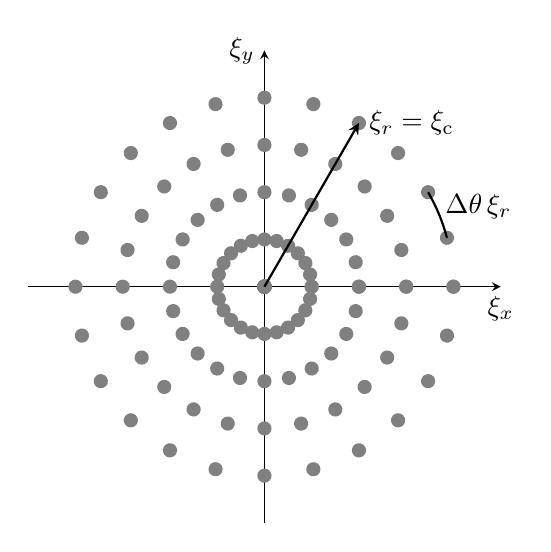
\begin{tikzpicture}[scale=3,>=stealth]
    % \clip(-1,-.35)rectangle(1,.35);
    \def\rr{0.9};
    \def\rrr{0.8};
    % axis
    \draw[->](0,-1)--(0,1)node[left,black]{$\xi_y$};
    \draw[->](-1,0)--(1,0)node[below,black]{$\xi_x$};
    % incident wave front
    \foreach \t in {0,15,...,360}{
      \foreach \xx in {0,0.2,...,\rrr}{
      \fill[gray,rotate=\t] (\xx,0) circle(0.03);} }
    \draw[thick,->](0,0)--(60:\rrr)node[right,black]{$\xi_r=\xic$};
    % angle
    \draw[thick] (15:\rrr) arc(15:30:\rrr) ;
    \draw[] (25:\rrr)node[right]{$\Delta\theta\,\xir$} ;
  \end{tikzpicture}
  \caption[Fourier space sampling under tomographic
  backprojection.]{Fourier space sampling upon backprojection of
    tomographic data according to the Fourier slice theorem.  The
    number $N$ of projections required to maintain detector resolution
    after backprojection, is determined by the angular sampling
    density at maximum spatial frequency $\xir=\xic$ matching the
    radial sampling density $\frac{2\xic}{N_x}$, $N_x$ being the
    number of horizontal detector pixels.}
  \label{fig:fourier-space-sampling}
\end{figure}
%%%%%%%%%%%%%%%%%%%%%%%%%%%%%%%%%%%%%%%%%%%%%%%%%%%%%%%%%%%%%%%%%%%%%%
Having derived expressions \cref{eq:fbp,eq:radon-inversion} for the
reconstruction of a function from its projections, the question arises
of the minimum number of projections required to maintain detector
resolution after tomographic reconstruction.  Therefore, we appeal to
the Fourier slice theorem again.  Each projection acquired under an
angle $\Theta$ corresponds to a slice in Fourier space at an angle
$\theta = \Theta+\frac{\pi}{2}$ as depicted in
\cref{fig:fourier-slice}.  Thus having obtained $N$ projections over
an angular range of \SI{180}{\degree} at a constant angle increment
$\Delta \Theta = \Delta \theta$, Fourier space is filled up
accordingly with slices as illustrated in
\cref{fig:fourier-space-sampling}.  Consider a horizontal detector
line of length $L$, effective pixel size $\Delta x$, and number of
pixels $N_x=\frac{L}{\Delta x}$.  Along such a slice, the maximum
spatial (cut-off) frequency reads $\xic=\frac{1}{2\Delta x}$, the
sampling density is $\frac{1}{L}$, and the number of (equidistant)
sampling points is that of the detector line $N_x$.  To maintain
detector resolution after backprojection the angular sampling density
at cut-off frequency $\xic$ should not fall below the radial
sampling density.  Thus $\frac{\pi \xic}{N}\le\frac{2\xic}{N_x}$ and
the minimum number of projections is given as
\begin{equation}
  \label{eq:num-proj}
  N \ge \frac{\pi}{2} N_x \;.
\end{equation}


\subsection{Coherence}
\label{sec:coherence}

In this section we consider the generation of (transverse) spatial
coherence from an incoherent source induced by the process of
propagation, with the essential result given by the van~Cittert-Zernike
theorem \cite{Wolf,BornWolf}.  As in \cref{sec:wave-packet}, we
consider quasi-monochromatic light with the amplitude of its plane
wave components differing appreciably from zero only within a
bandwidth $\Delta\omega$ about the mean frequency $\omega_0$,
\begin{equation}
  \label{eq:quasimono-2}
  \frac{\Delta\omega}{\omega_0}\ll 1 \;.
\end{equation}
From optical experiments on Michelson interferometers \cite{Wolf} it
is known that the appearance of fringes in the detection plane, which
is a manifestation of temporal coherence, is observed only as long as
the time delay $\Delta t$, introduced between the beams which are
brought to interfere, is less than
\begin{equation}
  \label{eq:coherence-time}
  \Delta t \le \frac{2\pi}{\Delta\omega} \;.
\end{equation}
For $\Delta t>\frac{2\pi}{\Delta\omega}$ spectral components within
the quasi-monochromatic wave packet run out of phase and cancel each
other on average.  Thus, $\Delta t$ is called coherence time and the
corresponding path delay is referred to as longitudinal coherence
length
\begin{equation}
   \label{eq:coherence-length-longitudinal}
   l_l = v \Delta t \approx v \frac{2\pi}{\Delta\omega} \;,
\end{equation}
where $v=\frac{c}{n}$ is the velocity of light in the medium of
propagation with $n=\const$ and $c$ being the speed of light in
vacuum, see \cref{eq:phase-velocity,eq:refractive-index}.  \Eg{} at an
X-ray energy of $E=\SI{30}{keV}$ and a monochromatisation of \num{e-4}
resulting in a bandwidth of $\Delta\omega=\SI{4.56e16}{s^{-1}}$, the
coherence length in vacuum ($v=c$) has a value of $l_l
=\SI{0.413}{\micro m}$, which is \eg{} considerably less than that of
optical lasers ranging from centimetres to kilometres.

%%%%%%%%%%%%%%%%%%%%%%%%%%%%%%%%%%%%%%%%%%%%%%%%%%%%%%%%%%%%%%%%%%%%%%
\begin{figure}
  \centering
  \small
  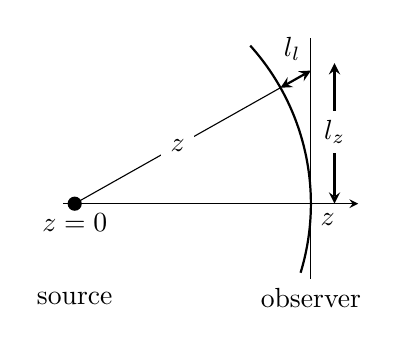
\begin{tikzpicture}[scale=3,>=stealth]
    \def\yy{0.7};
    \def\yyl{-0.4};
    \def\rrr{1};
    \def\ang{42};
    \def\angl{-17};
    % opical axis
    \draw[->](-0.05,0)--(\rrr+0.2,0);
    % SOURCE
    \fill[](0,0)circle(0.03)node[below]{$z=0$};
    \draw[](0,\yyl) node[]{source};
    % WAVE
    \draw[thick] (\ang:\rrr) arc(\ang:\angl:\rrr) ;
    \draw[](0,0)-- (0.7*\ang:\rrr);
    \draw[](0.7*\ang:\rrr/2)node[fill=white!100]{$z$};
    % OBSERVATION PLANE
    \draw[](\rrr,0)+(0,\yyl)--+(0,\yy)(\rrr,0)node[below right]{$z$};
    \fill[](\rrr,\yyl) node[fill=white!1000]{observer};
    % COHERENCE LENGTH LONGITUDINAL
    \draw[<->,thick](0.7*\ang:\rrr)--(\rrr,{\rrr*tan(0.7*\ang)})
    node[above left]{$l_l$};
    % COHERENCE LENGTH TRANSVERSE
    \draw[thick,<->](1.1*\rrr,0)+(0,0)--+(0,0.85*\yy);
    \draw[](1.1*\rrr,0)+(0,0.87*\yy/2)node[fill=white!100]{$l_z$};
  \end{tikzpicture}
  \caption[Emergence of a transverse coherence limit from a
  quasimonochromatic source.]{Emergence of a transverse coherence
    limit $l_z$ upon propagation of a spherical wave packet emitted
    from a quasi-monochromatic point source with longitudinal
    coherence length $l_l$ and a distance $z$ afar from the plane at
    $z$.  On the other hand, for a given transverse coherence length
    $l_z$, the bandwidth of the source imposes a lower bound on $z$.}
  \label{fig:longitudinal-coherence}
\end{figure}
%%%%%%%%%%%%%%%%%%%%%%%%%%%%%%%%%%%%%%%%%%%%%%%%%%%%%%%%%%%%%%%%%%%%%%

Considering a point source which emits a quasi-monochromatic spherical
wave packet, a longitudinal coherence length translates into a
transverse coherence length upon propagation, see
\cref{fig:longitudinal-coherence}.  In a given plane at a distance $z$
afar from the source, coherent interference can only arise from points
within this plane which exhibit a relative path delay of the incident
wave of less than
\begin{equation}
  \label{eq:quasi-mono-coherence-limit}
  l_l \ge \sqrt{z^2+l_z^2} - z 
  = z \sqrt{ 1 + \lrp{ \frac{l_z}{z} }^2} - z
  \approx \frac{l_z^2}{2 z} 
\end{equation}
and thus are separated less than $l_z \le \sqrt{2 R l_l }$.  For the
above value of $l_l =\SI{0.413}{\micro m}$ and at a distance
$z=R=\SI{100}{m}$, the emergent transverse coherence length is $l_z =
\SI{9.1}{mm}$.  In turn, for interference to occur at a given
transverse coherence length $l_z$, the finite bandwidth of radiation
emitted by a quasimonochromatic source imposes a lower bound on $z$ as
\begin{equation}
  \label{eq:minimum-distance}
  z \ge  \frac{l_z^2}{2 l_l}\;.
\end{equation}

Because of the great rapidity of light oscillations in the visible or
X-ray regime, the instantaneous intensity $\Psi^*\Psi$ of a wave field
$\Psi$ is technically inaccessible.  Only the intensity averaged over
time intervals $T$ can be measured
\begin{equation}
  \label{eq:time-averaged-intensity}
  \avg{\Psi(\vecr,t)^*\Psi(\vecr,t)}_t \equiv 
  \frac{1}{2 T}\int_{-T}^T\Intd{t} \Psi(\vecr,t)^*\Psi(\vecr,t) \;.
\end{equation}
For time intervals much larger than the reciprocal bandwidth,
$T\gg\frac{1}{\Delta \omega}$, we may formally let $T\to\infty$ as
\begin{equation}
  \label{eq:time-averaged-intensity-infty}
  I(\vecr) \equiv \lim_{T\to\infty} \frac{1}{2 T}
  \int_{-T}^T\Intd{t} \Psi(\vecr,t)^*\Psi(\vecr,t) \;.
\end{equation}
Using the ergodicity theorem \cite{Boltzmann1898}, the time average of
a quantity $Q$, such as in \cref{eq:time-averaged-intensity}, can be
replaced by the ensemble average \cite{Wolf}
\begin{equation}
  \label{eq:ensemble-average}
  \avg{Q(t)}_t = \avg{Q(t)}_e \equiv 
  \lim_{N\to\infty} \frac{1}{N}\sum_{k=1}^{N}Q\ho{k}(t)\;,
\end{equation}
where $Q\ho{k}$ denotes a particular realisation within an ensemble
$\{Q\ho{k}\}$.  In the remainder of this section we thus denote the
expectation value of a quantity $Q$ simply as $\avg{Q}$.

A generalisation of the definition of intensity is given by the mutual
coherence function $\Gamma$.  It is defined as the cross correlation
of the field $\Psi$ at distinct space-time points $(\vecr_1,t)$ and
$(\vecr_2,t+\tau)$ as
\begin{equation}
  \label{eq:mutual-coherence}
  \Gamma(\vecr_1,\vecr_2,\tau) \equiv
  \avg{\Psi^*(\vecr_1,t)\Psi(\vecr_2,t+\tau)} \;.
\end{equation}
The mutual coherence function at equal times is called mutual
intensity
\begin{equation}
  \label{eq:mutual-intensity}
  J(\vecr_1,\vecr_2)\equiv  \Gamma(\vecr_1,\vecr_2,0) \equiv
  \avg{\Psi^*(\vecr_1,t)\Psi(\vecr_2,t)} \;.
\end{equation}
The mutual intensity normalised by the intensities at $\vecr_1$ and
$\vecr_2$ is usually referred to as the complex degree of coherence
\begin{equation}
  \label{eq:complex-degree}
    j(\vecr_1,\vecr_2) \equiv 
    \frac{J(\vecr_1,\vecr_2)}{\sqrt{I(\vecr_1)I(\vecr_2)}} \;.
\end{equation}
Obviously, the degree of coherence exhibits a global maximum at
$\vecr_1=\vecr_2$.  From
\cref{eq:mutual-intensity,eq:mutual-coherence} the intensity reads as
\begin{equation}
  \label{eq:intensity-3}
  I(\vecr) \equiv J(\vecr,\vecr) \;.
\end{equation}


\subsubsection{Van Cittert-Zernike theorem}
\label{sec:van-cittert-zernike}

%%%%%%%%%%%%%%%%%%%%%%%%%%%%%%%%%%%%%%%%%%%%%%%%%%%%%%%%%%%%%%%%%%%%%%
\begin{figure}
  \centering
  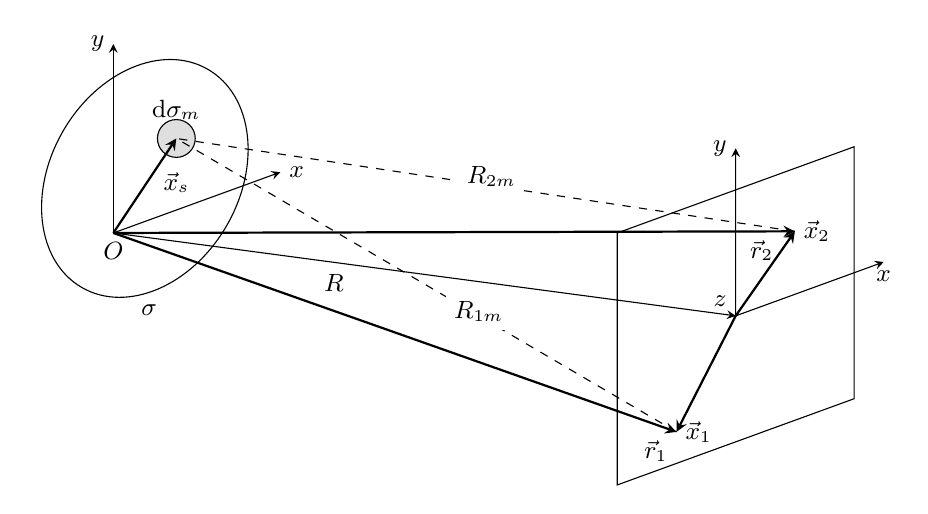
\begin{tikzpicture}[scale=0.8,>=stealth]
    \small
    \def\xx{1cm};    \def\yy{1.5cm};
    \draw[rotate=-30](0,\xx) ellipse(1.5cm and 2cm);
    \draw[] (\xx,\yy+0.15cm)node[above] {$\difd\sigma_m$} 
    (0.3,-1)node[below right]{$\sigma$};
    \fill[gray!25,%opacity=0.6
    ] (\xx,\yy) circle(0.3cm);
    \draw[] (\xx,\yy) circle(0.3cm);
    \draw[dashed] (8,-1)+(20:3cm)node[right]{$\vecx_2$} -- (\xx,\yy);
    \draw[] (6,0.9)node[fill=white!100]{$R_{2 m}$};
    \draw[dashed] (8,-3.5)+(20:1cm)node[right]{$\vecx_1$} -- (\xx,\yy);
    \draw[] (5.8,-1.25)node[fill=white!100]{$R_{1 m}$};
    \draw[thick,->] (0,0) -- (\xx,\yy);
    \draw[] (\xx,\yy)+(0,-0.7)node[]{$\vecx_s$};
    \draw[->] (0,0) -- (0,3)node[left]{$y$};
    \draw[->] (0,0) -- (20:2.82cm)node[right]{$x$};
    \draw[xshift=8cm,yshift=-4cm] (0,4) -- (0,0) -- (20:4) --+(0,4) -- cycle ;
    \draw[<->,xshift=8cm,yshift=-4cm] 
    (0,2)++(20:2cm)+(0,2.66)node[left]{$y$}--+(0,0)
    --+(20:2.5cm)node[below]{$x$};
    \draw[<-] (8,-2)+(20:2cm) -- (0,0)node[below]{$O$};
    \draw[](8,-2)+(20:2cm)node[above left]{$z$};
    % vecxip
    \draw[thick,<-] (8,-3.5)+(20:1cm)--(9.8794,-1.3160);
    \draw[thick,<-] (8,-1)+(20:3cm)--(9.8794,-1.3160);
    \draw[] (3.5,-0.8)node{$R$};
    % 3D vectors
    \draw[thick,<-] (8,-3.5)+(20:1cm) -- (0,0);
    \draw[] (8,-3.5)+(20:1cm)node[below left]{$\vecr_1$};
    \draw[thick,<-] (8,-1)+(20:3cm) -- (0,0);
    \draw[] (7.8,-1)+(20:3cm)node[below left]{$\vecr_2$};
  \end{tikzpicture}
  \caption[Van Cittert-Zernike theorem in the far field.]{Notation
    relating to the far-zone version of the van Cittert-Zernike
    theorem.  An extended planar source, situated at the origin $O
    (z=0)$ and described by the source function $\sigma$, incoherently
    emits quasi-monochromatic radiation of frequency $\omega_0$ and
    bandwidth $\Delta \omega$.  The source is divided into elements
    $\difd\sigma_m$ which, statistically independent from each other,
    emit an electromagnetic disturbance $\Psi_m$.  Vectors in the
    source plane are denoted $\vecr_m=(\vecx_s,0)$.  The plane of
    observation at $z=R$ is taken to be parallel to the source plane.
    Vectors in the observation plane are denoted
    $\vecr_i=(\vecx_i,R)$.  The distance between an source element at
    $\vecr_m$ and a point in the observation plane at $\vecr_i$ is
    denoted $R_{i m}$.  In the limit of a continuous source we let
    $R_{1 m}\to R_1$ and $R_{2 m}\to R_2$. }
  \label{fig:van-cittert-zernike}
\end{figure}
%%%%%%%%%%%%%%%%%%%%%%%%%%%%%%%%%%%%%%%%%%%%%%%%%%%%%%%%%%%%%%%%%%%%%%

In the following we will determine the mutual intensity and the
complex degree of coherence for light emitted from an extended,
incoherent and quasi-monochromatic source.  Consider an extended
planar source situated at the origin $O$ and described by the source
function $\sigma$ as in \cref{fig:van-cittert-zernike}.  The linear
extent of the source and the detector shall be small compared to the
distance $R$ between source and observer.  The source is divided
into elements $\difd\sigma_m$ located at $\vecr_m$.  Each source
element is assumed to emit quasi-monochromatic light of frequency
$\omega_0$ and bandwidth $\Delta\omega$ such that there is no
correlation between wave trains emanating from distinct elements
$\difd\sigma_m$.  The medium between source and observer is considered
to be homogeneous ($n=\const$).  Let $\Psi_m$ be the electromagnetic
disturbance produced by a source element $\difd\sigma_m$ as shown in
\cref{fig:van-cittert-zernike}.  The total field $\Psi$ at a position
$\vecr_i$ is given by the sum of $\Psi_m$ as
\begin{equation}
  \label{eq:total-field}
  \Psi(\vecr_i,t) = \sum_m \Psi_m(\vecr_i,t) \;.
\end{equation}
The mutual intensity of \cref{eq:mutual-intensity} then reads
\begin{equation}
  \label{eq:incoherent-j}
  \begin{split}
      J&(\vecr_1,\vecr_2) = \avg{\Psi^*(\vecr_1)\Psi(\vecr_2)} 
      \\ &= \sum_m \avg{\Psi^*_m(\vecr_1,t)\Psi_m(\vecr_2,t)} 
      + \mathop{\sum\!\sum}_{m\neq n} 
      \avg{\Psi^*_m(\vecr_1,t)\Psi_n(\vecr_2,t)} \;.
  \end{split}
\end{equation}
If we assume the light emitted from different source elements to be
statistically independent (mutually incoherent) and of zero mean
value, the second term in the last of \cref{eq:incoherent-j} vanishes
as
\begin{equation}
  \label{eq:uncorrealted-fields}
  \avg{\Psi^*_m(\vecr_1,t)\Psi_n(\vecr_2,t)} 
  = \avg{\Psi^*_m(\vecr_1,t)}\avg{\Psi_n(\vecr_2,t)} 
  = 0 \;.
\end{equation}
The distance between the observation point at $\vecr_i$ and a source
element $\difd\sigma_m$ at $\vecr_m$ is denoted $R_{i
  m}=\abs{\vecr_i-\vecr_m}$, see \cref{fig:van-cittert-zernike}.
Furthermore, we assume the disturbance emitted from an source element
$\difd\sigma_m$ to be a spherical harmonic wave of (complex)
amplitude $a_m(t)$.  The field $\Psi_m$, emitted from an element
$\difd\sigma_m$ at a time $t-\frac{R_{i m}}{v}$, is observed at
$\vecr_i$ at a later time $t$.  Thus we have
\begin{equation}
  \label{eq:source-wave}
  \Psi_m(\vecr_i,t) = a_m\lrp{t-\frac{R_{i m}}{v}} 
  \frac{\expb{-\ii\omega_0\lrp{t-\frac{R_{i m}}{v}}}}{R_{i m}} \;.
\end{equation}
Substituting \cref{eq:source-wave} into \cref{eq:incoherent-j} and
using \cref{eq:uncorrealted-fields}, the mutual intensity reads
\begin{equation}
  \label{eq:incoherent-j-2}
  \begin{split}
    J&(\vecr_1,\vecr_2)
    \\ & = \sum_m
    \avg{a^*_m\lrp{t-\tfrac{R_{1 m}}{v}} a_m\lrp{t-\tfrac{R_{2 m}}{v}}}
    \frac{\expb{-\ii\omega_0
        \lrp{\frac{R_{2 m}-R_{1 m}}{v}}}}{R_{1 m} R_{2 m}} 
    \\ & = \sum_m
    \avg{a^*_m\lrp{t} a_m\lrp{t-\tfrac{R_{2 m}-R_{1 m}}{v}}}
    \frac{\expb{-\ii\omega_0
        \lrp{\frac{R_{2 m}-R_{1 m}}{v}}}}{R_{1 m} R_{2 m}} \;,
  \end{split}
\end{equation}
where we have exploited the time-shift invariance of
\cref{eq:time-averaged-intensity-infty}.  Amplitude variations within
path differences $\abs{R_{2 m}-R_{1 m}}$ smaller than the longitudinal
coherence length of \cref{eq:coherence-length-longitudinal} will
average out in \cref{eq:incoherent-j-2}.  Thus, for $\abs{R_{2 m}-R_{1
    m}}<l_l$, we may neglect the retardation term $\frac{R_{2 m}-R_{1
    m}}{v}$ in the argument of $a_m$.  The quantity $\avg{a^*_m(t)
  a_m(t)}$ represents the intensity of the radiation emitted from the
source element $\difd\sigma_m$.  Let $I(\vecr_m)$ denote the intensity
emitted per unit area $\difd\sigma_m$ of the source. Then we have
\begin{equation}
  \label{eq:source-sum-to-int}
  \avg{a^*_m(t)a_m(t)}  = I(\vecr_m)\difd\sigma_m \;.
\end{equation}
In the limit of a continuous source, \cref{eq:incoherent-j-2}
becomes
\begin{equation}
  \label{eq:incoherent-j-3}
  \begin{split}
    J(\vecr_1,\vecr_2) & = \sum_m \avg{a^*_m(t) a_m(t)}
    \frac{\expb{-\ii k\lrp{R_{2 m}-R_{1 m}}}}{R_{1 m} R_{2 m}}
    \\ & = \int_\sigma \Intd{\sigma} I(\sigma)
    \frac{\expb{-\ii k(R_2-R_1)}}{R_1 R_2} \;,
  \end{split}
\end{equation}
where $R_{i m}\to R_i$ denotes the distance between a point on the
source at $\vecr_m$ and the observation point at $\vecr_i$, and
$k=\frac{\omega_0}{v}=n\frac{\omega_0}{c}$ is the (mean) wave number
in the medium, see \cref{eq:dispersion}.  Normalising the right-hand
side of \cref{eq:incoherent-j-3} by the intensities at $\vecr_1$ and
$\vecr_2$, we obtain the complex degree of coherence 
(\cref{eq:complex-degree}) as
\begin{equation}
  \label{eq:van-cittert-zernike}
  \begin{split}
    j(\vecr_1,\vecr_2) = 
    \frac{1}{\sqrt{I(\vecr_1)I(\vecr_2)}} 
    \int_\sigma \Intd{\sigma} I(\sigma)
    \frac{\expb{-\ii k (R_2-R_1)}}{R_2 R_2} \;,
  \end{split}
\end{equation}
with
\begin{equation}
  \label{eq:point-intensity}
  I(\vecr_i) = J(\vecr_i,\vecr_i) = 
  \int_\sigma \Intd{\sigma}  \frac{I(\sigma)}{R_i^2}
\end{equation}
being the averaged intensity at $\vecr_i$.
\Cref{eq:van-cittert-zernike} is called van Cittert-Zernike theorem.

\subsubsection{Van Cittert-Zernike theorem in the far field}
\label{sec:van-cittert-zernike-far-field}

In the far zone of the source and for observation points in a plane
parallel to the source plane, the van-Cittert-Zernike theorem takes on
a simpler form.  The position vectors in the observation plane at
$z=R$ and the source plane at $z=0$ are written as
$\vecr_i=(\vecx_i,R)$ and $\vecr_m=(\vecx_s,0)$, respectively, where
$R$ is the distance between these planes, see
\cref{fig:van-cittert-zernike}.  For values of $R$ being large in
comparison to the local extend of the source and the transverse area
of observation, the distance $R_i$ between a point on the source and a
point in the observation plane can be approximated by its Taylor
series to leading order as
\begin{equation}
  \label{eq:r-approximation}
  R_i = \sqrt{(\vecx_i-\vecx_s)^2 + R^2} 
  \approx R + \frac{(\vecx_i-\vecx_s)^2}{2 R} \;.
\end{equation}
The path difference then follows as
\begin{equation}
  \label{eq:path-difference}
  R_2 - R_1 \approx \frac{\vecx_2^2-\vecx_1^2}{2R} 
  - \frac{(\vecx_2-\vecx_1)\cdot\vecx_s}{R} \;.
\end{equation}
Furthermore, we define a phase
\begin{equation}
  \label{eq:phase-factor}
  \psi \equiv k\frac{\vecx_2^2-\vecx_1^2}{2R} \;.
\end{equation}
Approximating the denominator under the integral in
\cref{eq:van-cittert-zernike} by $R^2$ and substituting
\cref{eq:path-difference} into \cref{eq:van-cittert-zernike}, the
far-field version of the van Cittert-Zernike theorem follows as
\begin{equation}
  \label{eq:van-cittert-zernike-far-field}
  j(\vecr_1,\vecr_2) = 
  \frac{\expp{\ii\psi}}{\int_\sigma \Intdd{\vecx_s}I_s(\vecx_s)} 
  \int_\sigma\Intdd{\vecx_s}
 \expp{\tfrac{\ii k}{R}(\vecx_2-\vecx_1) \cdot \vecx_s}I_s(\vecx_s) \;,
\end{equation}
where $I_s(\vecx_s)\equiv I(\vecr_m)$ denotes the intensity at the
source plane, and $\difd^2\vecx_s=\difd\sigma$ the corresponding
surface element.  Thus, if the linear dimension of the source and the
distance $\abs{\vecx_2-\vecx_1}$ are small compared to $R$, the
complex degree of coherence is, apart from a phase and normalisation
factor, equal to the Fourier transform of the intensity distribution
across the source
\begin{equation}
  \label{eq:van-cittert-zernike-far-field-prop}
  j(\vecr_1,\vecr_2) 
  \propto \ft{ I}_s\lrp{ \frac{\vecx_2-\vecx_1}{\lambda R} } \;,
\end{equation}
where $\ft{I}_s \equiv \F I_s$ demands the Fourier transform of $I_s$
as in \cref{eq:ft-xi-2}.


\subsubsection{Incoherently illuminated object}
\label{sec:incoherent-illumination}

In \cref{sec:ctf}, the following expression for the forward propagated
spectral intensity is derived in Fresnel theory and under the
assumption of perfect spatial coherence
\begin{equation}
  \label{eq:guigay-coh-1}
  \begin{split}
    \ft{I}_z\hon{coh}(\vecxip) = 
     \int \Intdd{\vecxp}\exp{(-\ii 2\pi\vecxp\vecxip)} 
    \Psi_0\lrp{\vecx^- } \Psi^*_0\lrp{\vecx^+ } \;.
  \end{split}
\end{equation}
Here, $\vecxp$ denotes a transverse position vector, $\vecxip$ the
conjugate Fourier coordinate, and $\vecx^\pm = \vecxp\pm\tfrac{\lambda
  z}{2}\vecxip$.  To account for partial coherence, we have to replace
$I\hon{coh}_z$ in \cref{eq:guigay-coh-1} with its expectation value
$I(\vecr)\equiv I_z(\vecxp) = \avgn{I\hon{coh}_z}$.  Fourier
transformation and expectation value
(\cref{eq:time-averaged-intensity-infty}) commute and thus can be
interchanged.  If the longitudinal extent of the object is small
compared to distances $R$ and $z$, we may assume the projection
approximation to hold.  The wave field $\Psi_0$ upon object exit can
then be expressed in terms of the incident wave field
$\Psin\equiv\Psi_\omega\hon{in}$ and the transmission function
$T\equiv T_\omega$ as in \cref{eq:transmission}.  Thus, we may rewrite
\cref{eq:guigay-coh-1} as
\begin{equation}
  \label{eq:guigay-coh-2}
  \begin{split}
    \ft{I}_z(\vecxip) 
    & = \int \Intdd{\vecxp}\e{-\ii 2\pi\vecxp\vecxip}
    \avg{ \Psi_0\lrp{\vecx^-}\Psi^*_0\lrp{\vecx^+} } 
  \\ & = \int \Intdd{\vecxp}\e{-\ii 2\pi\vecxp\vecxip} \avg{
    T\lrp{\vecx^-}T^*\lrp{\vecx^+} 
    \Psin\lrp{\vecx^-}{\Psin}^*\lrp{\vecx^+} } 
  \\ & = \int \Intdd{\vecxp}\e{-\ii 2\pi\vecxp\vecxip} 
    T\lrp{\vecx^-}T^*\lrp{\vecx^+}
      \avg{ \Psin\lrp{\vecx^-}{\Psin}^*\lrp{\vecx^+ } } \;.
  \end{split}
\end{equation}
In the last line of \cref{eq:guigay-coh-2} we have used that the
transmission function is independent of the source statistics and can
be moved out of the expectation value.  The expectation value in the
last line of \cref{eq:guigay-coh-2} is identified with the mutual
intensity (\cref{eq:mutual-intensity}) of the incident wave field as
\begin{equation}
  \label{eq:incident-mutual-intensity}
    J\hon{in} = \avg{ \Psin\lrp{\vecx^-}{\Psin}^*\lrp{\vecx^+ } } \;.
\end{equation}
In the far field of the source we can use
\cref{eq:van-cittert-zernike-far-field} for the normalised mutual
intensity $j\hon{in}$.  If we assume the source intensity $I_s$ to be
normalised, we may omit the normalisation factor in $j\hon{in}$ and
thus use $j\hon{in}$ instead of $J\hon{in}$ in
\cref{eq:incident-mutual-intensity}.  The only position dependent
quantity appearing in \cref{eq:van-cittert-zernike-far-field} is the
phase factor $\psi$ entailing a rescaling of Fourier coordinates in
\cref{eq:guigay-coh-2}.  The rescaled Fourier transform $\ft{I}_s$ in
\cref{eq:van-cittert-zernike-far-field} depends on relative
coordinates only and thus can be moved out of the Fourier integral in
\cref{eq:guigay-coh-2}.  Hence, we have
\begin{equation}
  \label{eq:guigay-coh-3}
  \begin{split}
    \ft{I}_z(\vecxip) 
    & = \int \Intdd{\vecxp}\e{-\ii 2\pi\vecxp\vecxip} 
    T\lrp{\vecx^-}T^*\lrp{\vecx^+} j\hon{inc}(\vecx^-,\vecx^+)
    \\ &  = \ft{I}_s\lrp{\tfrac{\vecx^+-\vecx^-}{\lambda R}}
    \int\Intdd{\vecxp}\e{-\ii 2\pi\vecxp(\frac{R+z}{R})\vecxip} 
    T\lrp{\vecx^-}T^*\lrp{\vecx^+}
    \\ &  = \ft{I}_s\lrp{\tfrac{z}{R} \vecxip}
    \int\Intdd{\vecxp}\e{-\ii 2\pi\vecxp M \vecxip} 
    T\lrp{\vecx^-}T^*\lrp{\vecx^+} \;,
  \end{split}
\end{equation}
where have introduced the magnification factor $M$ as
\begin{equation}
  \label{eq:magnification}
   M \equiv \frac{z+R}{R} \;,
\end{equation}
see also \cref{fig:cone-beam-magnification}.  Furthermore, we define
the defocusing distance $D$ as
\begin{equation}
  \label{eq:defocus}
  D \equiv \frac{z}{M} = \frac{z R}{z + R} \;.
\end{equation}
The argument $\vecx^\pm$ then reads $\vecx^\pm\equiv\vecxp \pm
\tfrac{\lambda D M}{2}\vecxip$.  Using \cref{eq:guigay-coh-1} and the
definitions of $M$ and $D$, \cref{eq:guigay-coh-3} simplifies as
\begin{equation}
  \label{eq:guigay-incoherent}
    \ft{I}_z(\vecxip) = \ft{I}_s\lrp{\tfrac{z}{z+R} M\vecxip}
    \ft{I}_D\hon{coh}(M\vecxip) \;.
\end{equation}
In the far field of the source and for moderate propagation distances,
we may approximate $M\approx 1$, $D\approx z$, and $z+R\approx R$.
\Eg{} for in vivo scans performed at beamline station 32-ID-B at
\ac{aps} as described in \cref{sec:qp-tomo-invivo}, we have
$R=\SI{70}{m}$ and $z=\SI{0.7}{m}$, and thus a negligible
magnification of $M=\SI{1}{\percent}$.  Then
\cref{eq:guigay-incoherent} becomes
\begin{equation}
  \label{eq:guigay-incoherent-far-field}
    \ft{I}_z(\vecxip) = \ft{I}_s\lrp{\tfrac{z}{R}\vecxip}
    \ft{I}_z\hon{coh}(\vecxip) \;.
\end{equation}
Using the convolution theorem (\cref{eq:convolution-theorem-xi}) we
can express the intensity arising from an incoherent source as
\begin{equation}
  \label{eq:intensity-incoherent-far-field}
  I_z(\vecxp) = \lrp{\frac{R}{z}}^2 \int\Intdd{\vecxp'}
   I_s\lrp{\frac{R}{z}\vecxp'}  I_z\hon{coh}(\vecxp-\vecxp') \;.
\end{equation}


\subsubsection{Circular source}
\label{sec:circular-source}

Let us consider \cref{eq:van-cittert-zernike-far-field} for a circular
source of radius $s$ and constant intensity.  In this case the
integration in \cref{eq:van-cittert-zernike-far-field} can be carried
out \cite{BornWolf} and one finds the complex degree of coherence to
be given by
\begin{equation}
  \label{eq:circular-source}
  j(\vecr_1,\vecr_2) = \expp{\ii\psi}\frac{2 J_1(\nu)}{\nu} \;,
\end{equation}
where $J_1$ denotes the Bessel function of the first kind and first
order.  The argument of $J_1$ in \cref{eq:circular-source} is
\begin{equation}
  \label{eq:argument-j1}
  \nu \equiv k s\frac{\absn{\vecx_2-\vecx_1}}{R} \;.
\end{equation}
Apart from the phase factor, \cref{eq:circular-source} is identical to
the Airy formula of the Fraunhofer diffraction pattern originating
from a circular aperture uniformly illuminated by coherent light, see
\cref{sec:fraunhofer}.  The function $\frac{J_1(\nu)}{\nu}$ steadily
decreases from unity at $\nu = 0$ to zero at $\nu=\num{3.83}$.  Thus
there is complete incoherence for points separated by a distance
\begin{equation}
  \label{eq:incoherence}
  \abs{\vecx_2-\vecx_1} 
  = \frac{\num{3.83} R}{k s} 
  \approx \frac{\num{0.61} R \lambda}{s} \;.
\end{equation}
At $\nu =1$ the value of $\frac{J_1(\nu)}{\nu}$ has decreased to
\num{0.88} which is typically regarded as a permissible departure from
ideal coherence.  The corresponding transversal coherence length for a
circular shaped source of constant intensity reads
\begin{equation}
  \label{eq:coherence-length-circular}
  l_\perp\hon{circ}
  = \frac{R}{k s} 
  = \frac{\lambda R}{2\pi s} 
  \approx \frac{\num{0.16} \lambda R}{s} \;.
\end{equation}
% The dependencies in \cref{eq:coherence-length-circular} are understood as
% follows.  $\propto R$: as a spherical wave, emitted by single elements within
% the source, propagates the wave front extends

\subsubsection{Gaussian shaped source}
\label{sec:gaussian-source}

Let us now consider a symmetric, Gaussian shaped source of standard
deviation $\sigs$ and peak intensity $I_0$
\begin{equation}
  \label{eq:gaussian-source}
  I_s(\vecx_s) = 
  \frac{I_0}{2\pi\sigs^2} \expp{-\frac{\vecx_s^2}{2\sigs^2}} \;.
\end{equation}
The Fourier transform of the source function appearing in the
far-field version of the van Cittert-Zernike theorem
(\cref{eq:van-cittert-zernike-far-field}) yields again a Gaussian
function
\begin{equation}
  \label{eq:gaussian-source-ft}
  \ft{I}_s(\tfrac{\vecx_2-\vecx_1}{\lambda R})
  = I_0  \expp{-2 \lrb{ \frac{\pi\sigs\abs{\vecx_2-\vecx_1}}{\lambda R} }^2 }  \;.
\end{equation}
Thus, the complex degree of coherence reads
\begin{equation}
  \label{eq:gaussian-source-j}
  j(\vecr_1,\vecr_2) = \exp(\ii \psi)
  \expp{ -2 \lrb{ 
      \frac{ \pi\sigs\abs{\vecx_2-\vecx_1} }{ \lambda R } }^2 } \;.
\end{equation}
Identifying the source size $s$ with the \ac{fwhm} of the Gaussian
profile in \cref{eq:gaussian-source} as
\begin{equation}
  \label{eq:fwhm-source}
  s = \fwhm(I_s) = 2\sqrt{2\ln{2}}\sigs\approx\num{2.355}\,\sigs \;,
\end{equation}
we may define the transverse coherence length as the value where of
the degree of coherence $\abs{j(\vecr_1,\vecr_2)}$ has dropped to
$\frac12$.  The transverse coherence length of a Gaussian shaped
source then reads
\begin{equation}
  \label{eq:coherence-length-gaussian}
  l_\perp\hon{Gauss}
  = \sqrt{\frac{\ln{2}}{2}}\frac{\lambda R}{\pi \sigs} 
  = 2\ln{2}\frac{\lambda R}{\pi s}
  = \num{0.441}\frac{\lambda R}{s} \;.
\end{equation}
Note the factor of $4\ln{2}=\num{2.773}$ compared to the coherence
length of a circular source (\cref{eq:coherence-length-circular}).
\Eg{} at an X-ray energy of \SI{30}{keV} ($\lambda=\SI{4.13e-11}{m}$),
a source-to-detector distance of $R=\SI{100}{m}$, and a source
diameter of $s=\SI{100}{\micro m}$, the transverse coherence length
takes on a value of $l_\perp\hon{Gauss}= 4 \ln{2}\times
l_\perp\hon{circ} = 4\ln{2}\times\SI{6.58}{\micro m} =
\SI{20.66}{\micro m}$.  For convenience, we define the transverse
coherence length as
\begin{equation}
  \label{eq:coherence-length}
  l_\perp \equiv \frac{\lambda R}{2 s} \;.
\end{equation}

% Coherence length formula can be understood composed using heuristic
% considerations. proportional to R: as spherical waves emitted by
% single points within the source propagate, the wave front extends,
% proportional to a^-1: obvious, as for a->0 we have a point source
% with perfect spatial coherence in the far field; proportional to
% lambda: the smaller lambda the faster wave fronts originating from
% different points on the source run out of phase (remember the
% summation/integration over source elements in the derivation of the
% VCT

%%%%%%%%%%%%%%%%%%%%%%%%%%%%%%%%%%%%%%%%%%%%%%%%%%%%%%%%%%%%%%%%%%%%%%
\begin{figure}
  \centering
  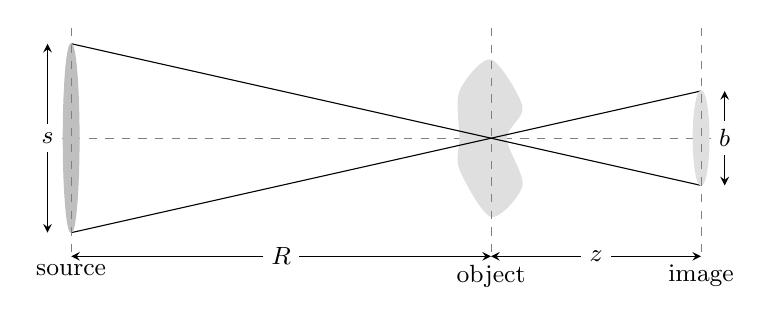
\begin{tikzpicture}[scale=2,>=stealth]
    \small
    % Parameters
    \def\zposo{2.666cm};
    \def\zposi{4cm};
    \def\yposh{-0.75cm};
    \def\yy{0.6cm};
    % optical axis
    \draw[help lines,dashed] (-0.1,0) -- (\zposi+0.1cm,0);
    % object
    \begin{scope}[xshift=\zposo,scale=1]
    \fill[color=gray!25,%opacity=1
    ] plot [smooth cycle] coordinates
    {(-0.2,0) (-0.2,0.3) (0,0.5) (0.2,0.2) (0.1,0) (0.2,-0.3) (0,-0.5)
      (-0.2,-0.2) };
    \end{scope}
    % rays
    \draw[](0,-\yy)--(\zposi,\yy/2);
    \draw[](0,\yy)--(\zposi,-\yy/2);
    % vertical lengths
    \draw[<->] (-.15,\yy)--(-0.15,-\yy);
    \draw[] (-0.15,0)node[fill=white!100]{$s$};
    % finite source
    \filldraw[color=gray!50,%opacity=0.6
    ] (0,0)ellipse(0.05cm and \yy);
    % vertical lengths image
    \draw[<->] (\zposi+0.15cm,\yy/2)--(\zposi+0.15cm,-\yy/2);
    \draw[] (\zposi+0.15cm,0)node[fill=white!100]{$b$};        
    % image
    \filldraw[color=gray!25,%opacity=1
    ] 
    (\zposi,0)ellipse(0.05cm and \yy/2);
    % vertical dashed lines
    \draw[dashed,help lines] (0,\yy+0.1cm)--(0,\yposh)
    node[below,black]{source};
    \draw[dashed,help lines] (\zposo,\yy+0.1cm) -- (\zposo,\yposh)
    node[below,black]{object};
    \draw[dashed,help lines] (\zposi,\yy+0.1cm) -- (\zposi,\yposh)
    node[below,black]{image};
   % length
    \draw[<->] (0,\yposh)--(\zposo,\yposh);
    \draw[] (\zposo/2,\yposh)node[fill=white!100]{$R$};
    \draw[<->] (\zposo,\yposh)--(\zposi,\yposh);
    \draw[] (\zposi/2+\zposo/2,\yposh)node[fill=white!100]{$z$};
  \end{tikzpicture}
  \caption[Geometrical blurring of image points induced by the finite
  extent of the illuminating source.]{Geometrical blurring induced by
    an extended source of diameter $a$ situated at distance $R$ from
    the object.  Object points imaged in the detector plane at a
    distance $z$ from the object are blurred by a factor $b=\frac{s
      z}{R}$ according to the intercept theorem.}
  \label{fig:geometrical-blurring}
\end{figure}
%%%%%%%%%%%%%%%%%%%%%%%%%%%%%%%%%%%%%%%%%%%%%%%%%%%%%%%%%%%%%%%%%%%%%%

\subsubsection{Source blurring}
\label{sec:source-blurring}

The finite extent of the source introduces a blur of object points at
the detector as illustrated in \cref{fig:geometrical-blurring}.  It
follows from the intercept theorem that the blur $b$ of image points
is given by
\begin{equation}
  \label{eq:source-blur}
  b = \frac{s z}{R} \;,
\end{equation}
where $z$ denotes the distance between sample and detector.  This
effect is experimentally demonstrated in
\cref{fig:intensity-sequence-anka}, depicting a sequence of (flat-field
corrected) intensity maps recorded with beamline TopoTomo at
\ac{anka}.  There, intensity contrast diminishes as propagation
distance is increased above $z\gtrsim\SI{0.5}{m}$.  Substituting the
source diameter by virtue of \cref{eq:coherence-length} into
\cref{eq:source-blur}, the blur relates to the coherence length as
\begin{equation}
  \label{eq:source-blur-coherence}
  b = \frac{\lambda z}{2 l_\perp} \;.
\end{equation}

The (Gaussian) blurring of object points imaged at the detector plane
can be described by means of a convolution of the coherent image,
arising from a point source, with a Gaussian function.  Let $I_b$
denote the blurred version of the coherent intensity $I$ given as
\begin{equation}
  \label{eq:image-blurred}
  \begin{split}
      I_b(\vecxp) = I \conv G & \equiv 
      \int\Intdd{\vecxp'} G(\vecxp') I(\vecxp-\vecxp')
      \\ & = \iF\lrb{ (\F {G})\, (\F {I})  }  \;,
  \end{split}
\end{equation}
where the convolution theorem of \cref{eq:convolution-theorem-xi} was
used, and $\F$ demands Fourier transformation as in \cref{eq:ft-xi-2}.
The blurring filter $G$ is given by a normalised Gaussian function in
two dimensions as
\begin{equation}
  \label{eq:blur-filter}
  G(\vecxp) = 
  \frac{1}{2\pi\sigb^2} \expp{-\frac{\vecxp^2}{2\sigb^2}} \;,
\end{equation}
where $\sigb$ is the standard deviation.  The blurring length is
identified with the \acf{fwhm} of $G$ as
\begin{equation}
  \label{eq:fwhm}
  b = \fwhm(G) = 2\sqrt{2\ln{2}}\sigb\approx\num{2.355}\,\sigb \;.
\end{equation}
Comparing \cref{eq:image-blurred,eq:intensity-incoherent-far-field},
the blurring filter connects to the source function as
\begin{equation}
  \label{eq:blur-filter-source-function}
    G(\vecxp) = \lrp{\frac{R}{z}}^2 I_s\lrp{\frac{R}{z}\vecxp} \;.
\end{equation}
For a Gaussian shaped source as in \cref{eq:gaussian-source}, we have
\begin{equation}
  \label{eq:blur-filter-gaussian-source}
  G(\vecxp) = 
  \lrp{\frac{R}{z}}^2\frac{1}{2\pi\sigs^2} 
  \expp{ -\frac{1}{2\sigs^2} \lrp{\frac{R}{z}\vecxp}^2 } \;,
\end{equation}
where we have set $I_0=1$ because in
\cref{eq:intensity-incoherent-far-field} we assumed $I_s$ to be
normalised.  Comparing
\cref{eq:blur-filter,eq:blur-filter-gaussian-source} the blur is
identified with the source size as
\begin{equation}
  \label{eq:sigma-blur-source}
  \sigb = \frac{z}{R}\sigs \;,
\end{equation}
in compliance with \cref{eq:source-blur}. 
%Thus, we have deduced the intercept theorem from Maxwell's equation.

Let us now consider the effect of blurring on the spectrum of the
propagated intensity using \cref{eq:image-blurred}.  Since the Fourier
transform of a Gaussian function yields a Gaussian function, $\ft{G}$
acts as low\hyph pass filter on $\ft{I}$ attenuating high frequencies.
The Fourier transform of $G$ evaluates as
\begin{equation}
  \label{eq:blur-filter-ft}
  \ft{G}(\vecxip) \equiv 
  \int\Intdd{\vecx_1}\expp{\ii 2\pi\vecxip\cdot\vecx_1}G(\vecx_1)
  = \expp{-2 (\sigb\pi\vecxip)^2} \;.
\end{equation}

%%%%%%%%%%%%%%%%%%%%%%%%%%%%%%%%%%%%%%%%%%%%%%%%%%%%%%%%%%%%%%%%%%%%%%
\begin{figure}
  \centering
  \subfloat[$z=\SI{0.5}{cm}$]{
    \includegraphics*[height=.197\textwidth]
    {figures/IntensitySequenceANKA/int0005mm.png}}
  \subfloat[$z=\SI{18}{cm}$]{
    \includegraphics*[height=.197\textwidth]
    {figures/IntensitySequenceANKA/int0180mm.png}}
    \subfloat[$z=\SI{58}{cm}$]{
    \includegraphics*[height=.197\textwidth]
    {figures/IntensitySequenceANKA/int0580mm.png}}
  \subfloat[$z=\SI{108}{cm}$]{
    \includegraphics*[height=.197\textwidth]
    {figures/IntensitySequenceANKA/int1080mm.png}}
  \caption[Intensity contrast in dependence of propagation
  distance.]{Sequence of (flat-field-corrected) intensity maps with
    increasing propagation distance $z$.  (a-c) Increasing
    phase-contrast-induced enhancement of intensity contrast (see
    \cref{sec:phase-retrieval}).  (d) Intensity contrast diminishes
    upon a further increase of $z$ due to source blurring.  Data was
    acquired with bending-magnet beamline TopoTomo at \ac{anka} under
    parallel-beam incidence at an energy of $E=\SI{12}{keV}$, a
    bandwidth of $\Delta E=\num{e-2}E$ using a multilayer
    monochromator, an effective pixel size of $\Delta x =
    \SI{1}{\micro m}$, and an exposure time of $\Delta t=\SI{180}{s}$.
    The sample, an early-stage Xenopus frog embryo, was embedded in
    agarose within an Eppendorf tube of diameter \SI{0.6}{cm} to avoid
    large phase jumps at the object boundary and reduce large-scale
    absorptive effects.}
  \label{fig:intensity-sequence-anka}
\end{figure}
%%%%%%%%%%%%%%%%%%%%%%%%%%%%%%%%%%%%%%%%%%%%%%%%%%%%%%%%%%%%%%%%%%%%%%

We may use \cref{eq:blur-filter-ft} to define the blurring-induced
transverse cut-off frequency $\xib$ as the frequency where $\ft{G}$
has dropped to the value $\e{-1}$,
\begin{equation}
  \label{eq:cut-off-frequency-blurring-0}
  \xib = \frac{1}{\sqrt{2}\sigb\pi}
  = \frac{2\sqrt{\ln{2}}}{\pi b} 
  \approx \num{0.53} \frac{1}{b} \;,
\end{equation}
where we have substituted $\sigb$ from \cref{eq:fwhm}.  Demanding a
drop of $\frac12$ instead results in a slightly stronger cut-off
$\xib\approx \num{0.44}\frac{1}{b}$.  Using
\cref{eq:source-blur-coherence},  $\xib$ relates to the coherence
length as
\begin{equation}
  \label{eq:cut-off-frequency-coherence}
   \xib = 4\sqrt{\ln{2}}\frac{l_{\perp}}{\pi\lambda z} 
   \approx \num{1.06} \frac{l_\perp}{\lambda z} \;.
\end{equation}
For convenience, we define the blurring-induced cut-off frequency as
\begin{equation}
  \label{eq:cut-off-frequency-blurring}
  \xib \equiv  \frac{1}{2 b} \;,
\end{equation}
or in terms of the transverse coherence length 
\begin{equation}
  \label{eq:cut-off-frequency-blurring-coherence}
  \xib = \frac{l_{\perp}}{\lambda z} \;.
\end{equation}
\Cref{eq:cut-off-frequency-blurring-coherence} is in compliance with
the relation for the cut-off frequency directly obtained from the
expression for $\ft{I}_z\hon{coh}$ in \cref{eq:guigay-coh-1}.
Regarding the autocorrelation on the right-hand side of
\cref{eq:guigay-coh-1}, only those points in the transverse plane
contribute to $\ft{I}_z\hon{coh}$ that are separated less than
$\abs{\vecx^+-\vecx^-}\le\lambda z \abs{\vecxip}\submax$.  The maximum
frequency $\abs{\vecxip}\submax$ is either set by the detector
resolution to $\xic=\frac{1}{2\Delta x}$ or by
\cref{eq:cut-off-frequency-blurring}.

%%%%%%%%%%%%%%%%%%%%%%%%%%%%%%%%%%%%%%%%%%%%%%%%%%%%%%%%%%%%%%%%%%%%%%
%%%%%%%%%%%%%%%%%%%%%%%%%%%%%%%%%%%%%%%%%%%%%%%%%%%%%%%%%%%%%%%%%%%%%%

\section{Microscopic interactions of X-rays and matter}
\label{sec:interaction}

Hitherto the interaction of light with matter were only taken into
account macroscopically in terms of the refractive index.  In this
section we will consider the interaction of X-rays and matter on the
atomic level.  This will allow us to relate the electron density
distribution to the refractive index.  The basic processes of the
interaction of light with matter are scattering and absorption of a
photon by an electron, obeying indeterministic rules that conspire
towards determinism at macroscopic scales, which is either considered
to be free or bound in an atom or molecule.  Thus an understanding of
the structure of atoms and matter is required.  Presently, the best
tested and efficient framework to address this is quantum mechanics.
To precisely describe the interaction of light and matter, quantum
mechanics has to be extended to quantum field theories involving the
second quantisation of gauge and particle fields \cite{Tomonaga1946,
  Schwinger1948a, Schwinger1948b, Feynman1949a, Feynman1949b,
  Feynman1950, Dyson1949}.  The processes of scattering and absorption
will be discussed in the \cref{sec:scattering,sec:absorption},
respectively.

\subsection{Scattering}
\label{sec:scattering}

The fundamental scattering unit of a photon in an atom or molecule is
the electron.  In the classical description the electron is
accelerated by an incident electromagnetic wave and commences to
oscillate, thereby emitting secondary electromagnetic waves of the
same far-field wave length as that of the incident field.  We thus are
dealing with an elastic scattering process which, in the limit of free
electrons, is called Thomson scattering.  This is the dominant
scattering process for X-rays.  In the case of inelastic scattering,
when energy is transferred from the photon to the electron, there is
no classical electrodynamic description and a quantum mechanical
treatment is mandatory.  This is know as Compton effect.

First, we will consider a semi-classical treatment of the scattering
process where a time-harmonic electromagnetic wave is incident on an
electron which is bound in an atom.  Let the electric field of the
incident wave at the position of the electron be
\begin{equation}
  \label{eq:incident-electric-field}
     \vecE_i=\vecE_0\exp(-i\omega t) \;,
\end{equation}
where $\vecE_0$ is a constant amplitude.  To a good approximation the
electron can be considered to behave under the influence of a
restoring force $-\hook\vecr$, where $\hook$ denotes the force
constant according to Hooke's law and $\vecr$ the displacement vector
with respect to the equilibrium position of the electron.  A
dissipative force resisting the motion accounts for damping effects,
\eg{} due to the emission of radiation or collisions between atoms.
This force reads $-g\vecv$, where $g$ is the damping coefficient and
$\vecv=\frac{\difd\vecr}{\difd t}$ denotes the electron's velocity
vector.  The Lorentz force acting on a particle which carries a charge
$q$ and moves with a velocity $\vec{v}$ in an electric and
magnetic field, $\vecE$ and $\vecB$, is given by
\begin{equation}
  \label{eq:lorentz}
  \vec{F} = q\left(\vecE + \vec{v}\times \vecB\right) \;.
\end{equation}
Disregarding magnetic interactions, the driving Lorentz force reduces
to $q\vecE$.  The forces exerted on the electron of charge $q=-e$
imply the well-know equation of motion of a damped harmonic
oscillator, driven by a periodic force:
\begin{equation}
  \label{eq:equation-of-motion}
  m\ddot{\vecr}+g\dot{\vecr}+\hook\vecr = -e\,\vecE_i\;.
\end{equation}
A particular solution to \cref{eq:equation-of-motion} is
\begin{equation}
  \label{eq:particular-solution}
  \vecr = \frac{-e\vecE_i}{m(\omega_0^2-\omega^2)-\ii\omega g}\;,
\end{equation}
where the angular frequency $\omega_0=\sqrt{\frac{\hook}{m}}$ denotes
the resonance or absorption frequency of the undamped system which is
related to electronic transitions in atoms and molecules.  The
occurrence of such frequencies at discrete values is a consequence of
quantum mechanics.  We now assume a given distribution of electrons
described by the electron density $\ed$.  Let each electron contribute
a dipole moment  $-e\vecr$ to the total polarisation $P$.
Neglecting the contributions from the nuclei, the total polarisation
reads
\begin{equation}
  \label{eq:P}
  \vecP = -e\ed\vecr = 
  \frac{e^2\ed\vecE_i}{m(\omega_0^2-\omega^2)-\ii\omega g} \;.
\end{equation}
From \cref{eq:susceptibility} we have $\vecP=\epsilon_0\chi_e\vecE_i$.
The dielectric susceptibility and, via \cref{eq:refractive-index}, the
refractive index $n$ follow as
\begin{equation}
  \label{eq:electric-susceptibility}
  \chi_e = n^2 - 1 
  = \frac{1}{\epsilon_0}\frac{e^2\ed}
  {\me(\omega_0^2-\omega^2)-\ii\omega g} \;.
\end{equation}
Thus, we have related the microscopic electron density distribution to
the macroscopic refractive index.  For vanishing frequencies of the
driving electromagnetic field the refractive index approaches
\begin{equation}
  \label{eq:zero-frequency}
  n^2(\omega=0)=1+\frac{e^2\ed}{\epsilon_0 \me\omega_0} \;.
\end{equation}
Note that for photon energies above the absorption edge,
$\omega>\omega_0$, and neglecting dissipative effects,
\cref{eq:electric-susceptibility} assumes negative values.
Introducing the classical electron radius defined as
\begin{equation}
  \label{eq:classical-electron-radius}
  r_e=\frac{e^2}{4\pi\varepsilon_0\me c^2}
  =\SI{2.828e-15}{m} = \SI{2.828e-5}{\angstrom} \;,
\end{equation}
we have
\begin{equation}
  \label{eq:refractive-index2}
  n^2 - 1  = - \frac{e^2\ed}{\epsilon_0 m(\omega^2-\omega_0^2)} 
  \approx  - \frac{e^2\ed}{\epsilon_0 m\omega^2} 
  = - \frac{4\pi r_e\ed}{k_0^2}  \;,
\end{equation}
with the wave number in vacuum $k_0=\frac{\omega}{c}$ (see
\cref{eq:wave-number-vacuum}).  For X-rays, the right-hand of
\cref{eq:refractive-index2} is close to zero and the refractive index
approximates
\begin{equation}
  \label{eq:refractive-index3}
  n  = 1 - \delta_\omega 
  = \sqrt{1- \frac{4\pi r_e \ed}{k^2}} 
  \approx 1 - \frac12\frac{4\pi r_e \ed}{k^2}
  = 1 - \frac{\lambda^2 r_e \ed}{2\pi} \;.
\end{equation}
Consequently, the refractive index is smaller than unity and the phase
velocity of light is larger than the speed of light in vacuum,
$v=\frac{c}{n}>c$.  This is yet in accordance with special relativity
because in regions of normal dispersion, where $\frac{\pd
  n}{\pd\omega}>0$, the propagation of energy takes place with the
group velocity 
\begin{equation}
  \label{eq:group-velocity-2}
  v_{\mathrm{g}} = \frac{\difd\omega}{\difd k}
  =\frac{c}{n(\omega)+\omega\frac{\pd n}{\pd\omega}}\;,
\end{equation}
which is smaller than $c$.  In regions of anomalous dispersion, \ie{}
close above the absorption edge, the group velocity cannot be
interpreted as the velocity at which energy propagates
\cite{Brillouin1960}.  As shown in \cref{fig:refractive-index}, the
refractive index approaches unity from below with increasing energy.
This is related to the fact that X-ray frequencies are usually higher
than the transition frequencies, except for those involving the inner
K- or L-shell electrons.  In the visible spectrum, where
$\omega\ll\omega_0$, the boundedness of electrons cannot be neglected.
Thus the refractive index is greater than unity and normal dispersion
is observed.
% , \ie{} the refractive index increases with increasing energy of the
% incident photon.

Let us sketch the derivation of the differential cross-section for the
elastic Thomson scattering of a linearly polarised electromagnetic
wave by a single free electron.  To evaluate the electric field which
is emitted by the electron, the retarded vector potential $\vecA$,
produced by the current density $\vecj$, is employed.  Working in
Lorenz gauge
\begin{equation}
  \label{eq:lorenz-gauge}
  \pd_\mu A^\mu = \frac{1}{c}\pd_t +\nabla\cdot\vecA =0 \;,
\end{equation}
the retarded potential reads as \cite{Jackson}
\begin{equation}
  \label{eq:retarded-vector-potential}
  \vecA(\vecr,t) = \frac{1}{4\pi\epsilon_0c^2}\int\Intddd{\vecr'}
  \frac{\vecj(\vecr',t-\abs{\vecr-\vecr'}/c)}{\abs{\vecr-\vecr'}} \;.
\end{equation}
The magnetic field is computes as $\vecB=\nabla\times\vecA$ and is
related to the electric field by $\abs{\vecE}=c\abs{\vecB}$.  The
current is identified with the induced dipole moments of the electrons
as $\vecj = \rho \vecv_p$, where $\rho$ is the electron charge density
and $\vecv_p\equiv\frac{\difd\vecr_p}{\difd t}$ with $\vecr_p$ given
by \cref{eq:particular-solution}.  Let the dipole be situated at the
origin and oscillate along a fixed axis.  The dipole approximation is
assumed, hence the electromagnetic field is considered in the far
field only.  In this region the only significant contribution of the
electric field is the polar component $E_\psi$ which is perpendicular
to the direction of observation and the magnetic field.
% and lies in the meridional plane.
It is given as
\begin{equation}
  \label{eq:electric-field-polar}
  E_\psi = -\frac{1}{4\pi\epsilon_0c^2} 
  \frac{-e}{r}\frac{\difd^2\vecr_p}{\difd t^2}\cos\psi \;,
\end{equation}
where $r=\abs{\vecr}$ is the distance to the observer, $\cos\psi$ the
polarisation factor, and $\psi$ the angle subtended by the unit vector
$\hat{\vecr}=\vecr/r$ and the plane perpendicular to the direction
$\hat{\vecr}_p=\vecr_p/\abs{\vecr_p}$ of the electric dipole
oscillation.  Thus the polarisation factor is calculated from
$\cos\psi=\abs{\hat{\vecr}_p\times\hat{\vecr}}$.  Since the electron
is considered free, the resonance frequency $\omega_0$ is set to
zero; or for photon energies far above the absorption edge we have
$\omega_0/\omega\approx0$.  Moreover, damping is neglected and 
the damping coefficient $g$ set to zero.  Thus,
$\frac{\difd^2\vecr_p}{\difd t^2}=\frac{-e}{m}\vecE_{i}$ and the ratio
of the radiated to incident electric field is found to be
\cite{Jackson}
\begin{equation}
  \label{eq:dipole-radiation}
  \frac{E_\psi}{\abs{\vecE_i}} = 
  -r_e\frac{\exp(\ii k_0 r)}{r}\cos\psi \;.
\end{equation}
Here $k_0=\frac{\omega}{c}$ is the incident wave number.  The minus
sign in \cref{eq:dipole-radiation} means that the phase of the
scattered wave emitted by the electron is shifted by $\pi$ with
respect to the incident wave.

From
\cref{eq:dipole-radiation,eq:differential-scattering-cross-section}
the differential cross-section for the incident radiation to be
scattered into a solid angle $\difd\Omega$ follows as
\begin{equation}
  \label{eq:thomson-electron}         
  \frac{\difd\sigma_T}{\difd\Omega}=r_e^2 \cos^2\psi \;.
\end{equation}
Therefore, the classical electron radius $r_e$ is also known as
Thomson scattering length.  Assuming a distribution of charges given
by the charge density $\rho$, \cref{eq:thomson-electron}
becomes
\begin{equation}
  \label{eq:thomson-rho}         
  \frac{\difd\sigma_T}{\difd\Omega} = 
  r_e^2 \cos^2\psi\, |f_0(\vec{q})|^2 \;.
\end{equation}
Here, the atomic form factor $f_0$ computes as the phase\hyph
weighted integral of $\rho$ and  thus involves the Fourier transform
of $\rho$ as
\begin{equation}
  \label{eq:form-factor}
  f_0(\vec{q})=
  \int\Intddd{\vec{r}}\rho(\vec{r})\exp(\ii \vec{q}\vec{r}) \;,
\end{equation}
where $\vec{q}=\vec{k_i}-\vec{k_f}$ denotes the momentum transfer
between incoming ($\vec{k_i}$) and scattered wave ($\vec{k_f}$).  When
the photon scatters off an atom in a molecule (or a unit cell), an
additional summation over the atomic form factors of individual atoms,
located at $\vec{r}_j$, is required.  The atomic form factor in
\cref{eq:thomson-rho} is then replaced with
\begin{equation}
  \label{eq:form-factor-molecule}
  f_o(\vecq) \to F(\vec{q}) = 
  \sum_{j} f_j(\vec{q})\exp(\ii\vec{q}\vec{r}_j)\;.
\end{equation}
For a crystal lattice constituting an array of unit cells, a
significant scattering signal is obtained only when the momentum
transfer coincides with a lattice vector $\vec{G}$ of the reciprocal
space.  Thus $\vec{q}=\vec{G}$, which is called Laue condition.
Summing over all unit cells of the crystal,
\cref{eq:form-factor-molecule} becomes the structure factor.

The total cross section for Thomson scattering owns a constant value
of
\begin{equation}
  \label{eq:thomson-cross-section}         
  \sigma_T = \frac{8\pi}{3}r_e^2 
  = \SI{0.665e-24}{cm^2} = \SI{0.665}{barn} \;.
\end{equation}
In terms of the Compton wave length $\lambda_C=\frac{h}{\me c}$ and
the fine-structure constant
$\alpha=\frac{1}{4\pi\epsilon_0}\frac{e^2}{\hbar c}$, the Thomson
cross-section reads $\sigma_T = \frac{8\pi}{3}
\frac{\alpha\lambda_C}{2\pi}^2$.

For photon energies considerably greater than the electron binding
energy the electron can be considered free and the atomic form factor
is to a good approximation given by $f_0$.  For energies less than the
electron binding energy resonant scattering behaviour is observed,
which can be accounted for by supplementing dispersion corrections to
$f_0$.  Then the atomic form factor is written as the sum of the
energy-independent part $f_0$ and the dispersion corrections $f'$ and
$f''$ which are due to bound-state effects of the electron in an
atom
\begin{equation}
  \label{eq:total-atomic-form-factor}
  f(\vec{q},\omega) = f_0(\vec{q})+ f'(\omega) +\ii f''(\omega) \;.
\end{equation}
The imaginary part $f''$ of \cref{eq:total-atomic-form-factor}
represents the dissipation in the system.  The extrema of the
dispersion corrections are encountered at energies corresponding to
the absorption edges of an atom.

In a quantum mechanical description the differential cross section for
elastic scattering can be calculated via Fermi's Golden rule which
states that the transition rate $w_{i\rightarrow f}$, \ie{} the
transition probability per unit time for the system to evolve from an
initial state $\ket{i}$ to a final state $\ket{f}$, provided by
first-order time-dependent perturbation theory, is given by
\cite{Sakurai}
\begin{equation}
  \label{eq:fermis-golden-rule}
  w_{i\rightarrow f}=\frac{2\pi}{\hbar}M_{f i}^2\delta(E_f-E_i)\;.
\end{equation}
The factor $M_{if}$ denotes the transition matrix element to be
computed from the interaction Hamiltonian $\mathcal{H}_{\mathrm{I}}$
by
\begin{equation}
  \label{eq:Mfi}
  M_{if}=\bra{f}\mathcal{H}_{\mathrm{I}}\ket{i} \;.
\end{equation}
If there is a group of final states $\{f\}$ with nearly the same
energy as the energy of the initial state $\ket{i}$ and with a density
of states $\rho(E)$ within an energy interval $(E,E+\difd E)$, the
left-hand side of \cref{eq:fermis-golden-rule} must be integrated with
$\int\Intd{E_f}\rho(E_f)$ to yield $w_{i\to\{f\}}$.  Given a beam of
flux density $\Phi_0$ incident on a sample, the differential cross
section for elastic scattering follows as
\begin{equation}
  \label{eq:scattering-cross-qm}
  \frac{d\sigma}{d\Omega} = 
  \frac{w_{i\to \{f\}}}{\Phi_0\Delta\Omega} = 
  \left(\frac{V}{2\pi}\right)^2\frac{\hbar^4}{c^4}
  \int\intd E_f \abs{M_{if}}^2E_f^2\delta(E_f-E_i)\;.
\end{equation}
Here, $V$ is the interaction volume introduced for normalisation
purposes, and $E_i$ and $E_f$ denote the initial and final energy of
the incident and the scattered photon, respectively.
The energy of the vector potential $\vecA$ is normalised to $E_i$
within the interaction volume $V$ via
\begin{equation}
  \label{eq:normalisation-condition}
  \int_V\Intddd{\vecr}\frac12
  \lrp{\epsilon_0\vecE^2+\frac{1}{\mu_0}\vecB^2} 
  = E_i = \hbar\omega
\end{equation}
such that $V$ drops out in
\cref{eq:scattering-cross-qm} because a cancellation between
$\abs{M_{if}}^2$ and the factor $V$ takes place.  The same holds for
\cref{eq:absorption-cross-qm}.  The interaction Hamiltonian of the
photon-electron system is given by
\begin{equation}
  \label{eq:hamiltonian-vector}
   \mathcal{H}_{\mathrm{I}} = 
   \frac{e \vecp\cdot\vecA}{\me}+\frac{e^2\vecA^2}{2\me} \;,
\end{equation}
where $\vecp=\vecp\subn{kin}-e\vecA$ is the electron's canonical
momentum and $\vecA$ the vector potential of the electromagnetic field
in physical Coulomb gauge.  $\vecp\subn{kin} = \me\vecv$ is the
kinematic momentum with $\vecv=\frac{\difd\vecr}{\difd t}$ denoting
the electron velocity.  Thomson scattering is related to the part of
the interaction Hamiltonian which is quadratic in the vector
potential.  This is because scattering involves the annihilation of
the incident photon state and the creation of the scattered photon
state when the vector potential is expressed in terms of annihilation
and creation operators acting on the state kets according the second
quantisation \cite{Ryder1996}.  The polarisation factor in
\cref{eq:thomson-rho} corresponds to the squared product of the
polarisation vectors of the incident and scattered photon, and the
form factor is given by
$f(\vec{q})=\bra{\vec{p}}\exp(\ii\vec{q}\vec{r})\ket{\vec{p}}$.

The vector potential $\vecA$ is defined only modulo gauge
transformations.  The full Hamiltonian is thus a gauge\hyph invariant
transforming term given by
\begin{equation}
  \label{eq:full-hamiltonian}
  \frac{\vecp\subn{kin}^2}{2\me} = 
  \frac{(\vecp -q\vecA)^2}{2\me} = 
    \frac{(\frac{1}{\ii\hbar}\nabla + e\vecA)^2}{2\me} \;.
\end{equation}
\Cref{eq:full-hamiltonian} is artificially decomposed into a
time-independent Hamilton $H_0$ of the undisturbed system and a
potentially time-dependent interacting part $H_I$.  If $H_0$ and $H_I$
are treated separately, each individual term is no longer gauge
invariant.  Nevertheless we may employ the vector potential as long as
we work in a physical gauge such as the Coulomb gauge.  The Coulomb
gauge, also called radiation gauge or transversal gauge, renders the
vector potential divergence free
\begin{equation}
  \label{eq:coulomb-gauge}
  \nabla\cdot\vecA(\vecr,t) = 0 \;.
\end{equation}
Then, in the absence of sources, the vector potential itself is
governed by the wave equation and the scalar potential by the Poisson
equation $\nabla^2\phi=-\rho(\vecr,t)/\epsilon_0$.  Thus $\phi$
represents the instantaneous Coulomb potential. %


Inelastic scattering is described by the Compton effect which involves
a transfer of energy from the photon to the electron.  The
corresponding change in wave length of the scattered photon is given
by
\begin{equation}
  \label{eq:compton-scattering}
  \lambda_f-\lambda_i=\lambda_C(1-\cos\theta)\;,
\end{equation}
where $\theta$ is the scattering angle and $\lambda_C$ 
the Compton scattering length defined as
\begin{equation}
  \label{eq:compton-length}
  \lambda_C=\frac{h}{\me c} = \SI{3.86e-13}{m} \;.
\end{equation}
Note that Compton scattering is incoherent, while Thomson scattering is
coherent (Bragg's law, Laue condition).  
% Indeterminism when \hbar pops out of vacuum 
The contribution of Compton
scattering to the total scattering cross section increases with
increasing energy.  The differential cross-section for photons
scattered from a single free electron in lowest order of quantum
electrodynamics is calculated by the Klein-Nishina formula
\cite{KleinNishina1929}.  The corresponding total cross section is
given as
\begin{equation}
  \label{eq:klein-nishina-cross-section}
  \begin{split}
      \sigma_{\mathrm{KN}} = 2\pi r_e^2\left(
    \frac{1+\eta}{\eta^2}
    \left[ \frac{2(1+\eta)}{1+2\eta} 
      -\frac{1}{\eta}\ln(1+2\eta) \right] \right.
    \\\left.+\frac{1}{2\eta}\ln(1+2\eta)-\frac{1+3\eta}{(1+2\eta)^2}
    \right) \;,
  \end{split}
\end{equation}
where $\eta$ denotes the ratio of the incident photon energy to the
electron rest energy as $\eta=\frac{E_\gamma}{\me c^2}$.  At
low-frequencies, $\eta\ll 1$, the Klein\hyph Nishina formula reduces
to the classical Thomson scattering formula of
\cref{eq:thomson-cross-section}.


\subsection{Absorption}
\label{sec:absorption}

The absorption of a photon by an atom is called photoelectric effect.
It is the extreme inelastic limit of Compton scattering.  During this
process photon energy is transferred to an electron which subsequently
is expelled from the atom being left ionised.  The photoelectric
effect is a manifestation of the quantisation of the electromagnetic
field energy.  The energy of the emitted photoelectron is proportional
to the frequency of the incident light, but not to its intensity
\cite{Einstein1905}.  Quantitatively, the average photoelectric
absorption is described in terms of the linear absorption coefficient
$\mu$.  According to Beer's law (\cref{eq:beers-law}), the attenuation
of an incident beam of intensity $I_0$ is given by
\begin{equation}
  \label{eq:beers-law-2}
  I(z) = I_0\exp(-\mu_\omega z)\;.
\end{equation}
The linear absorption coefficient is related to the absorption
cross-section $\sigma_a$ by
\begin{equation}
  \label{eq:absorption-cross}
  \mu_\omega=2k_0\beta_\omega = \rho_a\sigma_a 
  = \frac{\rho_m N_A}{A}\sigma_a\;,
\end{equation}
where $\rho_a$ is the atomic number density, $\rho_m$ the mass
density, $N_A$ Avogadro's number, and $A$ the atomic mass number.

Likewise Compton scattering the photoelectric absorption evades a
classical explanation and a quantum mechanical treatment is mandatory.
By means of Fermi's Golden Rule (\cref{eq:fermis-golden-rule}) the
absorption cross-section can be expressed in terms of the transition
matrix element $M_{if}$ of the interaction Hamiltonian as
\begin{equation}
  \label{eq:absorption-cross-qm}
  \sigma_a=\frac{w_{i\to\{f\}}}{\Phi_0} = 
  \frac{2\pi V}{\hbar c}\int\intd E_{\mathrm{pe}}|M_{if}|^2
  \rho(E_{\mathrm{pe}})\delta(E_{\mathrm{pe}}-(E_i-E_{\mathrm{b}}))\;,
\end{equation}
where $E_i$ is the energy of the incident photon, $E_{\mathrm{b}}$ the
electron binding energy, and $E_{\mathrm{pe}}$ the kinetic energy of
the photoelectron.  As for \cref{eq:scattering-cross-qm}, the
interaction volume $V$ is introduced for normalisation purposes and
cancels with $|M_{if}|^2$.  Here, $\{f\}$ indicates that the
integration is performed over the entire solid of $4\pi$ to account
for that the photoelectron can be expelled in all possible directions.
The matrix element for photoelectric absorption is related to the part
of the interaction Hamiltonian which is linear in the vector potential
\begin{equation}
  M_{if}=\frac{e}{m}\bra{f}\vecp\vecA\ket{i} \;,
\end{equation}
thus allowing for the annihilation of a photon.

Following photoelectric absorption and an expel of an electron from
the inner atomic shell, the created hole can be filled by either of
two distinct processes: (i) Fluorescent X-ray emission
\cite{Barkla1904}: the hole is filled by an electron from the outer
shell.  The transition entails the emission of a photon with an energy
equal to the difference in binding energies of the involved electronic
states.  The monochromatic radiation can be used as a fingerprint to
identify the atom which has emitted the fluorescent X-ray photon. (ii)
Auger electron emission \cite{Meitner1922}: alternatively to the
emission of fluorescent X-rays, the energy, released during the
transition of an outer shell electron to the inner shell, can be
transferred to another electron from the outer shell which
subsequently will be expelled from the atom.  This process is called
Auger effect.  The hole in the inner atomic shell can also be created
by $\gamma$-rays or charged particles such as electrons or positrons.

Away from absorption edges, the photoelectric absorption cross-section
is approximately proportional to $E^{-3}$.  For condensed matter and
close to an absorption edge the absorption spectrum exhibits a fine
structure which depends on the chemistry of the material.  This
phenomenon is exploited in experiments measuring the spectrum of the
\acf{XASF}, comprising \acf{XANES} and \acf{EXAFS}.  These two methods
give complementary structural information, the \ac{XANES} spectra
being sensitive to electronic structures and the symmetry of a metal
site, and \ac{EXAFS} spectra telling about numbers, types, and
distances to ligands and neighbouring atoms with respect to the
absorbing element \cite{KoningsbergerPrins}.
% XANES: multiple scattering of the photoelectron and resonances
% occur. the scattering amplitude at neighbouring atoms is high and
% wavelengths are larger than interatomic distances
%
% EXAFS: single scattering of the (high-energy) photoelectron at the
% electrons of the neighbouring atoms.  The wave function of the
% photoelectron is a superposition of the spherically outward
% travelling wave and the wave which is backscattered from the
% neighbouring atoms.
%fine structure in the absorption at energies greater than the
%threshold for electron release.
A detailed treatment of X-ray absorption and \ac{XASF} is given in
\cite{KoningsbergerPrins}.

Conventional X-ray imaging employing absorption contrast relies on the
strong dependence of the photoelectric absorption cross-section on the
atomic number $Z$ varying with $Z^4$.  The photoelectric effect is the
dominant contribution to the absorption cross-section for photon
energies much less than the electron rest mass of
$\me=\SI{511}{keV/c^2}$.

%%%%%%%%%%%%%%%%%%%%%%%%%%%%%%%%%%%%%%%%%%%%%%%%%%%%%%%%%%%%%%%%%%%%%%
%%%%%%%%%%%%%%%%%%%%%%%%%%%%%%%%%%%%%%%%%%%%%%%%%%%%%%%%%%%%%%%%%%%%%%


\section{Phase retrieval}
\label{sec:phase-retrieval}

% The mean of the phase is sometimes referred to as piston term.

% Alrady Zernike coined the term phase object for irregular structures
% causing diffraction not by unequal amplitede but by unequal optical
% light paths, \ie{} unequal phases \cite{Zernike1955}.

% On fringe thickness: In the edge-enhancement regime where intensity
% contrast is given by $g_z(x)=-\tfrac{\lambda z}{2\pi}$, the
% thickness of the evolving fringe is given by the sharpness of the
% the edge considered. In analogy, to the emittance of a
% electromagnetic disturbance from an antenna, the near field profile
% depends on the emitting material, in the far field, however, the
% profile is independent on the material.

In the following we consider phase variations induced in the exit wave
field by the interaction of hard, monochromatic, electromagnetic
radiation with the sample.  Furthermore, we confine our consideration
to the idealised situation of perfect spatial coherence and in the
absence of noise.  A treatment of the case subject to shot-noise
(Poisson) in the context of non-linear phase retrieval is given in
\cref{sec:qp}.

Numerous methods have been devised to retrieve the phase of an exit
wave (transmission function) from measurements of the associated
intensity.  Interferometric techniques rely on the interference of the
phase\hyph distorted wave front with an undistorted or biasing
reference beam \cite{Zernike1942a, Zernike1942b, BonseHart1965,
  Momose1995nima, BornWolf}.  Crystal interferometry \eg{} is based on
Bragg reflection (in Bragg or Laue geometry).  It requires an
extremely high stability of the experimental setup in order to prevent
spatial displacements down to atomic scales within the interferometer.
Unless the interferometer is build from a monolithic block, this
involves a meticulous alignment of the reflecting crystals.  An
alternative interferometric technique employs diffraction gratings,
which is much less prone to problems relating to the positioning and
stability of the setup \cite{Platt2001, David2002, Kohmura2003,
  Momose2003opex, Pfeiffer2006natphys}.  Diffraction enhanced imaging,
also know as Schlieren technique or analyser-based imaging, appeals to
the linear relation $\Delta \alpha = \frac{1}{k}\abs{\np\phi_0}$
between the angle $\Delta\alpha$, subtended by the diffracted beam to
the optical axis $z$, and the transverse derivative of the phase
$\np\phi_0$.  \footnote{ In \cref{sec:fresnel,sec:proj-approx} we
  found that, assuming forward propagation and constant absorption,
  the monochromatic exit wave field can be written in terms of the
  exit phase, $\phi_0$, as
\begin{equation}
  \label{eq:exit-wave-2} 
  \Psi_\omega(\vecr) = 
  \Psi_0\expp{\ii\phi_0(\vecxp)+\ii k z} \;,
\end{equation} 
with $\vecr=(\vecxp,z)$, see \cref{eq:transmission,eq:ansatz-env}.
From \cref{eq:exit-wave-2} and using the three-dimensional Fourier
representation of $\Psi_\omega$ and the Fourier derivative theorem,
the gradient $\nabla$ of the wave field relates to the wave vector
$\veck$ as
\begin{equation}
  \label{eq:nabla-k} 
  \begin{split}
    \nabla\,\Psi_\omega(\vecr) 
    & = \ii(\np\phi_0(\vecxp),k)\Psi_\omega(\vecr) 
    \\ & = \FO{^{-1}_\veck} \ii(\np\phi_0(\vecxp),k)
    \ft{\Psi}_\omega(\veck) 
    \\ & = \FO{^{-1}_\veck}(-\ii\veck)\ft{\Psi}_\omega(\veck) \;,
  \end{split}
\end{equation}
where $\np$ denotes the transverse two-dimensional gradient operator
with $\nabla=(\np,\pd_z)$.  From \cref{eq:nabla-k} the wave vector
reads as
\begin{equation}
  \label{eq:wave-vector-derivative}
  \veck =  -(\np\phi_0(\vecxp),k) \;.
\end{equation}
Assuming the angular deviations $\Delta\alpha$ of the diffracted beam
with respect to the incident wave propagating along $z$ to be
small (see \cref{fig:small-angle-approximation}), it follows from
\cref{eq:wave-vector-derivative,eq:pa} that
\begin{equation}
  \label{eq:small-angle-diffraction}
  \Delta\alpha \approx \sin\Delta\alpha 
  =\frac{\absn{\veckp}}{k} 
  = \frac{1}{k}\abs{\np\phi_0(\vecxp)} \;.
\end{equation}
} A quantitative analysis of the acquired rocking curves (intensity as
a function of $\Delta\alpha$) involves input from dynamical
diffraction theory (finite Darwin width)
\cite{Foerster1980,Davis1995,Bushuev1996,Luebbert2000,Nesterets2008}.
 
The majority of phase-sensitive imaging methods mentioned above
involves a scanning or stepping procedure.  This renders the
instrumental setup more demanding and less robust, and the data
acquisition slower and less dose efficient in comparison to
single\hyph measurement techniques.  On the other hand, free\hyph
space (or in\hyph line) propagation\hyph based phase\hyph contrast
imaging is free of additional optics and relies on the measurement of
a single intensity map at a single distance only
\cite{Snigirev1995,Wilkins1996}.  The acquired intensity pattern
emerges due to the self-interference of light diffracted at exiting
the object and propagating towards the detector (Fresnel theory).  To
retrieve the phase of the exit wave from measurements of the
propagated intensity poses an inverse problem, typically addressed in
linear approximations by appeal to the \acf{tie} \cite{Teague1982,
  Teague1983, Gureyev1995, Gureyev1996, Paganin1998, Gureyev2004,
  Nugent2005} or the \acf{ctf} \cite{Turner2004, Gureyev2006OptCommun,
  Gureyev2006apl}.

In the following sections we discuss the most widely used approaches
to single\hyph distance and single\hyph measurement phase retrieval.
In \cref{sec:tie,sec:ctf} we discuss linear models based on \ac{tie}
and \ac{ctf}, respectively.  \Cref{sec:duality} reviews the linear
algorithms of \cref{sec:tie,sec:ctf} in the context of the
phase-attenuation duality which assumes proportionality between
attenuation and phase.  \Cref{sec:regularisation} is concerned with
regularisation procedures for phase retrieval.

In the remaining part of this thesis we will omit the subscript
$_\omega$, indicating the dependence on energy, and introduce the
following notation for the sake of better readability:
\begin{equation}
  \label{eq:abbreviations}
  \begin{split}
       I_z(\vecxp) & \equiv I_\omega(\vecxp,z) \;,
       \\ \Psi_z(\vecxp) & \equiv \Psi_\omega(\vecxp,z) \;,
       \\ \phi_z(\vecxp) & \equiv \phi_\omega(\vecxp,z) \;,
       \\ B_z(\vecxp) & \equiv B_\omega(\vecxp,z) \;.
  \end{split}
\end{equation}


\subsection{Transport of intensity equation}
\label{sec:tie}

In \cref{sec:fresnel}, we derived the paraxial wave equation for a
wave field propagating within a static, homogeneous, and non\hyph
magnetic medium by virtue of the paraxial approximation.  The
$z$-evolution of the envelope of the wave field was found to be
governed by
\begin{equation}
  \label{eq:pwe-2}
  \left(\np^2 +2\ii k\pd_z\right)\Psi\env_{z}(\vecxp) = 0 \;,
\end{equation}
where $\np$ denotes the two-dimensional derivative transverse to the
optical axis and $k=\frac{2\pi}{\lambda}= n \frac{\omega}{c}$ with
$n=\const$ and $c$ the speed of light in vacuum.  In the following we
will omit the superscript $\env$ for the envelope of the wave field.
Rewrite the envelope field in terms of intensity and phase shift as
\begin{equation}
  \label{eq:tie-wave}
  \Psi_{z}(\vecxp)  
  = \sqrt{I_z(\vecxp)}\expb{\ii\phi_z(\vecxp)} \;,
\end{equation}
and substitute \cref{eq:tie-wave} into \cref{eq:pwe-2}.  The imaginary
part of the resulting equation is called \acf{tie}.  It reads
\cite{Teague1983,Rytov1989}
\begin{equation}
  \label{eq:tie}
  k\,\pd_z I_z(\vecxp) =
  -\np\cdot\lrb{I_z(\vecxp)\,\np\phi_z(\vecxp)} \;.
\end{equation}
Note that \cref{eq:tie} corresponds to a continuity equation of
Fresnel theory, see \cref{eq:continuity-fresnel}.  The corresponding
real part is given as
\begin{equation}
  \label{eq:pwe-real-0}
  2k\pd_z\phi_z(\vecxp)=
    \frac{\np^2\sqrt{I_z(\vecxp)}}{\sqrt{I_z(\vecxp)}}
    -\left(\np\phi_z(\vecxp)\right)^2\;.
\end{equation}
Employing \ac{tie} for phase retrieval takes into account only an
incomplete version of Fresnel theory.

The edge-enhancement regime is defined as the region of small
propagation distances where the intensity varies in an approximately
linear way in $z$.  For sufficiently small $z$ the derivative on the
left-hand side of \cref{eq:tie} can be expressed by a Taylor
expansion of $I_z(\vecxp)$ in $z$ truncated at linear order.  The
$z$-derivative then reduces to the forward difference quotient at
first order in $z$ as
\begin{equation}
  \label{eq:quotient}
  \pd_z I_z(\vecxp)\approx 
  \frac{I_{z+\Delta z}(\vecxp)-I_z(\vecxp)}{\Delta z} \;.
\end{equation}
Evaluating  \cref{eq:tie} for small values of $z$
and using \cref{eq:quotient}, we obtain the following relation between
the intensity at $z>0$ and the phase of the exit wave at $z=0$
\begin{equation}
\label{eq:tie-small-z}
  I_z(\vecxp)=I_0(\vecxp)
  -\frac{z}{k}\np\cdot\left(I_0(\vecxp)\,\np\phi_0(\vecxp)\right)\;.
\end{equation}
The actual signal is given by the intensity contrast $g_z$ defined as
\begin{equation}
  \label{eq:g}
   g_z(\vecxp) \equiv  g_\omega(\vecxp,z)
  =\frac{I_z(\vecxp)}{\Iin(\vecxp)}-1 \;.
\end{equation}


\subsubsection{Pure-phase objects}
\label{sec:tie-pure-phase}

%%%%%%%%%%%%%%%%%%%%%%%%%%%%%%%%%%%%%%%%%%%%%%%%%%%%%%%%%%%%%%%%%%%%%%
\begin{figure} 
  % Plot created from Matlab function phdFig_TransferFunctions
  \centering
  \small
  \psfragfig[width=0.8\textwidth,
  height=0.25\textheight]
  {figures/TransferFunction/Fig1}{  \small
    \psfrag{xlabel}[c][c]{$\;\abs{\vecxip}/\xic$}
    \psfrag{ylabel}[c][c]{Transfer function}
    \psfrag{0.2}{0.2} \psfrag{0.4}{0.4} \psfrag{0.6}{0.6} 
    \psfrag{0.8}{0.8} \psfrag{-2}{-2} \psfrag{-1}{-1} \psfrag{0}{0}
    \psfrag{1}{1} \psfrag{2}{2} \psfrag{3}{3} \psfrag{4}{4}
    \psfrag{data1}{$\tie$}
    \psfrag{data2}{$\ctf$}
  }
  \caption[Linear Transfer functions between phase and
  intensity.]{Radial dependence of transfer functions related to
    \cref{eq:linear-tie-phase,eq:ctf-phase}: $\tie(x) = 2x$ and
    $\ctf(x) = 2\sin x$ with $x=\pi\lambda z\vecxip^2$.  Energy was
    set to $E=\SI{12.4}{keV}$ ($\lambda=\SI{e-10}{m}$), propagation
    distance to $z=\SI{0.1}{m}$, and pixel size to $\Delta x =
    \SI{1}{\micro m}$.  The maximal (cut-off) frequency is given by
    $\xic=(2\Delta x)^{-1}$.  Thus $x=\frac{\pi\lambda z}{(2\Delta
      x)^2}\frac{\abs{\vecxip}^2}{\xic^2} =
    2.5\pi\frac{\abs{\vecxip}^2}{\xic^2}$, and $\ctf$ encounters two
    additional zero crossing compared to $\tie$.  See
    \cref{fig:phase-filter} for the inverted transfer functions.}
  \label{fig:transfer-function}
\end{figure}
%%%%%%%%%%%%%%%%%%%%%%%%%%%%%%%%%%%%%%%%%%%%%%%%%%%%%%%%%%%%%%%%%%%%%%


Here we consider a pure-phase object exhibiting a constant attenuation
$B_0$ at the exit plane.  The incident field $\Psi\supin$ impinging on
the sample is taken to be a plane wave of intensity
$I\supin=\absn{\Psi\supin}^2$.  For the intensity  at the exit plane
we have
\begin{equation}
  \label{eq:exit-intensity}
  I_0(\vecxp) = \Iin\exp(-2 B_0)  =\const \;.
\end{equation}
In this case,  intensity contrast reads 
\begin{equation}
  \label{eq:g-pure-phase}
   g_z(\vecxp) = \frac{I_z(\vecxp)}{I_{0}(\vecxp)}-1 \;,
\end{equation}
and  linearised \ac{tie} \eqref{eq:tie-small-z} becomes
\cite{Bremmer1952}
\begin{equation}
  \label{eq:tie-linear}
  g_z(\vecxp)=-\frac{z}{k}\np^2\phi_0(\vecxp)\;.
\end{equation}
\Cref{eq:tie-linear} states that out of given phase map at the object
exit, intensity contrast emerges at edges of the projected object and
strengthens with increasing propagation distance, see 
\cref{fig:intensity-sequence-anka,fig:fringe-evolution}.  An algebraic
inversion of \cref{eq:tie-linear} is obtained by means of the Fourier
derivative theorem (\cref{eq:fdt-k-n}) reading
\begin{equation}
  \label{eq:fourier-derivative}
  \np f(\vecxp) = \iF\lrb{ -\ii\veckp \F f(\vecxp) } \;,
\end{equation}
which holds for the Fourier transformation as defined in
\cref{eq:ft-k-2}.  Thus, a solution of the phase-retrieval problem
from a single-distance measurement at small $z$ is given by
\begin{equation}
  \label{eq:linear-tie-phase}
  \phi_0(\vecxp) = 
  \frac{k}{z} \iF\left[\frac{\ft{g}_z(\veckp)}{\veckp^{2}}\right] \;,
\end{equation}
provided that the singularity arising form the denominator at zero
frequency is properly regularised, see \cref{sec:regularisation}.  In
the following we will refer to phase retrieval based on
\cref{eq:linear-tie-phase} as linearised \ac{tie}.  Considering the
right-hand side of \cref{eq:linear-tie-phase}, it becomes evident that
the inversion of the Laplacian acts as a low-pass filter on the
intensity data suppressing high frequencies with a factor
$\veckp^{-2}$, see \cref{fig:transfer-function,fig:phase-filter} where
transfer functions and their regularised inverse functions are
plotted.  This is why linearised \ac{tie} phase retrieval performs
robust and is applicable even beyond the edge-enhancement regime
though at the expense of spatial resolution.  This will be analysed in
more detail in \cref{sec:qp-linear-models}.
% discussion of
% coherence, pixel size, noise, influencing resolution.
A numerically fast and efficient implementation is provided by
\cref{eq:linear-tie-phase} using fast \ac{fft}
algorithms.

%%%%%%%%%%%%%%%%%%%%%%%%%%%%%%%%%%%%%%%%%%%%%%%%%%%%%%%%%%%%%%%%%%%%%%
\begin{figure} 
  % Plots created from Matlab function phdFig_PhaseFilter
  \centering
  \small
  \psfragfig[
  width=0.8\textwidth,
  height=0.25\textheight
  ]
  {figures/PhaseFilter/Fig1}{\small
    \psfrag{xlabel}[c][c]{$\;\abs{\vecxip}/\xic$}
    \psfrag{ylabel}[c][c]{Inverse transfer function}
%    \footnotesize
    \psfrag{0.2}{0.2} \psfrag{0.4}{0.4} \psfrag{0.6}{0.6} 
    \psfrag{0.8}{0.8} \psfrag{1}{1} \psfrag{0}{0}
    \psfrag{-50}{-50} \psfrag{0}{0} \psfrag{50}{50} 
    \psfrag{data1}{$\tie$}
    \psfrag{data2}{$\ctf$}
  }
  \caption[Fourier space filter (regularised inverse transfer
  function) for standard phase retrieval.]{Radial dependence of
    regularised inverse transfer functions related to
    \cref{eq:linear-tie-phase,eq:ctf-phase}.  See
    \cref{fig:transfer-function} for the transfer functions itself.
    Using the regularisation of
    \cref{eq:zero-regularisation,eq:regularisation-sine}, the
    regularised inverse transfer functions read $\tie(x) =
    \frac12(x+\alpha)^{-1}$ and $\ctf(x) = \frac{\sgn{(\sin
        x)}}{2\abs{\sin x}+\alpha}$ with $x=\pi\lambda z\vecxip^2$.
    Energy was set to $E=\SI{12.4}{keV}$ ($\lambda=\SI{1e-10}{m}$),
    propagation distance to $z=\SI{0.1}{m}$, pixel size to $\Delta x =
    \SI{1}{\micro m}$, and the regularisation parameter to
    $\alpha=\num{e-2}$.  The maximal (cut-off) frequency is given by
    $\xic=(2\Delta x)^{-1}$.  Thus $x=\frac{\pi\lambda z}{(2\Delta
      x)^2}\frac{\abs{\vecxip}^2}{\xic^2} =
    2.5\pi\frac{\abs{\vecxip}^2}{\xic^2}$, and $\ctf$ encounters two
    additional singularities compared to $\tie$.  At $x=0$,
    $\ctf(0)=\tie(0)=\frac{1}{2\alpha}$, implying that regularisation
    rescales the mean value of the retrieved phase (see also
    \cref{sec:mean-phase}).}
  \label{fig:phase-filter}
\end{figure}
%%%%%%%%%%%%%%%%%%%%%%%%%%%%%%%%%%%%%%%%%%%%%%%%%%%%%%%%%%%%%%%%%%%%%%


\Cref{eq:tie-linear} was derived in several contexts \cite{Nugent1996,
  PaganinBook} and can also be obtained form the Fresnel diffraction
integral as in \cite{Bronnikov2002}.  Therefore we consider the Taylor
expansion of the exponential in the Fourier-space version of the
Fresnel propagator truncated at quadratic order in $\veckp$ as
\begin{equation}
  \label{eq:fresnel-propagator-expansion}
  \begin{split}
    (\F\Prop_F)(\veckp,z) 
    & = \frac{\exp(\ii k z)}{2\pi}\expp{-\frac{\ii z}{2k}\veckp^2} 
    \\ & \approx \frac{\exp(\ii k z)}{2\pi}
    \left(1-\frac{\ii z}{2k}\veckp^2 \right) \;.
  \end{split}
\end{equation}
By insertion of \cref{eq:fresnel-propagator-expansion} into the
Fourier representation of the Fresnel diffraction integral
(\cref{eq:fresnel}) and using the Fourier derivative theorem
(\cref{eq:fourier-derivative}), the intensity follows as
\begin{equation}
  \begin{split}
  \label{eq:fresnel-limit-0}
  I_z(\vecxp) 
  & = \abs{2\pi\, \iF\left[ \Prop_F \cdot\F \Psi_0\right]}^2
  \\ & =  \abs{\left(1 +  
      \frac{\ii z}{2k} \iF (\ii\veckp)^2 \F\right) \Psi_0}^2
  \\ & =  \abs{\left(1 +  \frac{\ii z}{2k} 
      \np^2 \right) \Psi_0}^2 \;.
  \end{split}
\end{equation}
To continue we evaluate the Laplacian as
\begin{equation}
  \np^2\Psi_0=\lrb{\ii(\np^2\phi_0)-(\np\phi_0)^2}\Psi_0 \;,
\end{equation}
and the modulus in \cref{eq:fresnel-limit-0} as
\begin{equation}
  \begin{split}
  \label{eq:fresnel-limit-1}
  I_z(\vecxp) & =  \abs{\left(1 +  \frac{\ii z}{2k} 
      \np^2 \right) \Psi_0}^2
  % \\ & = I_0\abs{ 1 - \tfrac{z}{2k} \np^2\phi -\ii\tfrac{z}{2k} (\np\phi)^2}^2 \;.
  \\ & = I_0\left[ 1 - 2\frac{z}{2k}\np^2\phi_0
    + \left(\tfrac{z}{2k}\np^2\phi_0\right)^2 
    + \left(\tfrac{z}{2k}\right)^2(\np\phi_0)^4 \right]
  \\ & = I_0\left[ 1 - \frac{z}{k}\np^2\phi_0 
    + \order(\phi_0^2) \right] \;.
  \end{split}
\end{equation}
Thus, to linear order in $\phi_0$, linearised \ac{tie}
\eqref{eq:tie-linear} is recovered.

Let us consider the validity regime of \cref{eq:tie-linear}.  For the
truncation in \cref{eq:fresnel-propagator-expansion} to be valid,
higher orders in the power\hyph series expansion of the exponential in
\cref{eq:fresnel-propagator-expansion} must be negligible.  The
following condition must then be satisfied for all accessible values
of $\veckp$:
\begin{equation}
  \label{eq:truncation-condition}
  1 \gg\ \abs{\frac12\frac{z}{2k}\veckp^2} \;.
\end{equation}
An upper limit of the transverse spatial frequency is set by the
linear size $\Delta x$ of the detector pixels to
$\abs{\veckp}\le\abs{\frac{2\pi}{2\Delta x}}$.  Thus condition
\eqref{eq:truncation-condition} reads
\begin{equation}
  \label{eq:truncation-condition-2}
  1 \gg\ \frac{\lambda z \pi}{8 (\Delta x)^2} \;.
\end{equation}
In a typical imaging experiment using propagation-based phase contrast
at an energy of $E=\SI{20}{keV}$ with a pixel size of $\Delta
x=\SI{1e-6}{m}$ and a moderate sample-to-detector distance of
$z=\SI{0.1}{m}$, the right-hand side of
\eqref{eq:truncation-condition-2} already assumes a value of 2.4.
Strictly speaking, the validity of linearised \ac{tie} is limited to
the very near field regime of Fresnel theory.  At the expense of an
ever decreasing spatial resolution, phase retrieval based on
\cref{eq:tie-linear} is applicable beyond the validity of
\cref{eq:truncation-condition-2} owing to its low-pass filter
characteristic.  Even though linearised \ac{tie} is applicable at
large phase shifts, the retrieved phase over- or underestimates the
exact phase, see \cref{fig:siemens-star-cuts,fig:siemens-star-thick}.
How to overcome this mismatch using a perturbative approach is subject
of \cref{sec:perturbation-theory}.

Within the edge-enhancement regime, where the validity of linearised
\ac{tie} \eqref{eq:tie-linear} is assured and appropriately models the
recorded data, the signal strength is typically low since intensity
contrast rises linearly with $z$, see
\cref{fig:fringe-evolution,fig:qp-2}(a).  Thus, if we cannot afford
long exposure times to acquire data of an acceptable \ac{snr}, we opt
for larger propagation distances to enhance the signal and thus 
\ac{snr}.  Then, however, the low-pass filtering behaviour, inherent
to the inversion of linearised \ac{tie}, impedes phase retrieval at a
high spatial resolution.  To do so we appeal to approaches based on
the \ac{ctf} relation, which will be discussed in the following
section.


\subsection{Contrast transfer function}
\label{sec:ctf}

An alternative approach to \ac{tie} related phase retrieval is based
on \acfp{ctf} which are closely related to transfers functions
encountered in optical and electron microscopy
\cite{Streibl1985,Kirkland1998}.  In Fourier space, \ac{ctf}
represents a local and linear relation between phase shift and
attenuation at the object-exit plane and the propagated intensity
contrast.  An important relation, valid in Fresnel theory, states that
the Fourier transformed intensity can be written as the Fourier
transform of a two-point autocorrelation of the exit wave field
(transmission function) \cite{Guigay1977,Guigay1978,Papoulis1974}.
The \ac{ctf} expression is derived from this relation by an expansion
of the transmission functions truncated at linear order in the
attenuation and in relative phase variations.  To derive the
autocorrelation relation, the convolution form of the Fresnel
diffraction integral is used twice to evaluate the intensity as
follows
\begin{equation}
  \label{eq:guigay-0}
  \begin{split}
    \ft{I}(\veckp) & \equiv (\F I)(\veckp) 
    \\ &= \F\lrb{ \Psi_z(\vecxp) \Psi_z^*(\vecxp) } 
    \\ &=\F\lrb{ (\Prop_F\conv\Psi_0)(\Prop^*_F\conv\Psi_0^*) } 
    \\ &=\F\lrb{\int\Intdd{\vecxp'}\int\Intdd{\vecxp''}
      \Psi_0(\vecxp')\Psi_0^*(\vecxp'')
      \Prop_F(\vecxp-\vecxp')\Prop^*_F(\vecxp-\vecxp'') } \;.
  \end{split}
\end{equation}
As the Fourier transformation only affects the propagators in the last
line of \cref{eq:guigay-0}, it can be evaluated yielding a
(two-dimensional) Dirac delta distribution (\cref{eq:dirac-xi-n}) as
\begin{equation}
  \label{eq:fourier-propagator}
  \begin{split}
    &\F\left[\Prop_F(\vecxp-\vecxp')\Prop^*_F(\vecxp-\vecxp'') \right]
    \\ &= \frac{2\pi}{(\lambda z)^2} 
    \expsb{\frac{\ii\pi}{\lambda z}(\vecxp'^2-\vecxp''^2)}
    \delta^2\left(\veckp
      +\frac{2\pi}{\lambda z}(\vecxp'-\vecxp'')\right)
    \\ &=\frac{1}{2\pi} \expsb{\frac{\ii\pi}{\lambda z}
      (\vecxp'^2-\vecxp''^2)}
    \delta^2\left(\vecxp' -\vecxp'' 
      + \frac{\lambda z}{2\pi}\veckp)\right) \;,
  \end{split}
\end{equation}
where we have used the scaling property of the Dirac delta
distribution, see \cref{eq:dirac-scaling}.  To proceed,
\cref{eq:fourier-propagator} is substituted into \cref{eq:guigay-0}
and the integration over $\vecxp'$ is performed.  The remaining
integration variable is shifted by $\vecxp''=\vecxp+\frac{\lambda
  z}{4\pi}\veckp$ yielding the Fourier transform of the two-point
autocorrelation of $\Psi_0$.  Thus we arrive at the final result
\begin{equation}
  \label{eq:guigay}
      \ft{I}_z(\veckp) = 
      \frac{1}{2\pi}\int \Intdd{\vecxp}\e{-\ii\,\vecxp\veckp} 
      \Psi_0\left(\vecxp-\frac{z}{2k}\veckp\right)
      \Psi^*_0\left(\vecxp+\frac{z}{2k}\veckp\right) \;.
\end{equation}
In statistical mechanics, the right-hand side of \cref{eq:guigay} is
known as Wigner distribution function introduced to account for
quantum mechanical corrections to the thermodynamic equilibrium
\cite{Wigner1932}.  \Cref{eq:guigay} is also closely related to the
ambiguity function in Fourier optics \cite{Papoulis1974,Guigay1978}.
Note that \cref{eq:guigay} is valid in the case of perfect spatial
coherence only.  In the situation of partial coherence the product
$\Psi_0{\Psi_0}^*$ has to be substituted by the ensemble average
quantity $\avg{\Psi_0\Psi^*_0}_e$ , see \cref{eq:ensemble-average} and
\cref{sec:coherence}.  Employing the Fourier transform defined in
ordinary instead of angular frequencies $\vecxip
=\frac{\veckp}{2\pi}$, \cref{eq:guigay} reads
\begin{equation}
  \label{eq:guigay-xi}
    \ft{I}_z(\vecxip) = 
    \int \Intdd{\vecxp}\e{-\ii 2\pi\vecxp\vecxip} 
    \Psi_0\left(\vecxp-\frac{\lambda z}{2}\vecxip\right) 
    \Psi^*_0\left(\vecxp+\frac{\lambda z}{2}\vecxip\right) \;,
\end{equation}
where we have used $k=\frac{2\pi}{\lambda}$.  Considering the
right-hand side of \cref{eq:guigay-xi} it becomes clear that intensity
contrast emerges due to the interference of points in the exit wave
field which are separated by a distance $\lambda z\abs{\vecxip}$
growing linearly in $z$.  With increasing $z$ small object scales such
as fine-structure edges increasingly contribute to the propagated
intensity pattern in terms of a multiplicity of fringes, see
\cref{fig:fringe-evolution} for the $z$-evolution of such a fringe
pattern.  Note that \cref{eq:guigay-xi} is tied to the full Fresnel
theory.  The Fraunhofer limit of the paraxial approximation would
yield a different relation between $\Psi_0$ and $\ft{I}_z$, see
\cref{sec:fraunhofer}.

%%%%%%%%%%%%%%%%%%%%%%%%%%%%%%%%%%%%%%%%%%%%%%%%%%%%%%%%%%%%%%%%%%%%%%
\begin{figure} 
  \centering
  \psfragfig[width=0.99\textwidth,height=0.33\textheight]
  {figures/FringeEvolution/Fig1}{
    \small
    \psfrag{ylabel2}[b][c]{
      \rotatebox[origin=c]{180}{Normalised intensity $I_z$}}
    \psfrag{ylabel}[c][c]{Phase $\phi_0$}
    \psfrag{xlabel}[c][c]{Pixel ($\mu m$)}
    \psfrag{1.5}{1.5}
    \psfrag{1.4}{1.4} \psfrag{1.3}{1.3} \psfrag{1.2}{1.2}
    \psfrag{1.1}{1.1} \psfrag{1}{1} \psfrag{0.9}{0.9}
    \psfrag{0.8}{0.8} \psfrag{0.7}{0.7} 
    \psfrag{0.2}{0.2} \psfrag{0.4}{0.4} \psfrag{0.6}{0.6} 
    \psfrag{-10}{-10} \psfrag{-20}{-20} 
    \psfrag{-30}{-30} \psfrag{-40}{-40} \psfrag{-50}{-50}
    \psfrag{-60}{-60} \psfrag{0}{0} \psfrag{10}{10} \psfrag{20}{20}
    \psfrag{30}{30} \psfrag{40}{40} \psfrag{50}{50} \psfrag{60}{60}
    \psfrag{data1}{$\phi_0:z=\SI{0}{m}$}
    \psfrag{data2}{$I_z:z=\SI{0.1}{m}$}
    \psfrag{data3}{$I_z:z=\SI{0.5}{m}$}
    \psfrag{data4}{$I_z:z=\SI{1.5}{m}$}
    \psfrag{data5}{$I_z:z=\SI{3.0}{m}$}
  }
  \caption[Evolution of fringes in the propagated intensity from an
  edge-like phase object in simulated forward propagation.]{Evolution
    of fringes in the intensity contrast from an edge-like phase
    object in simulated forward propagation.  Energy was set to
    $E=\SI{20}{keV}$ ($\lambda=\SI{6.12e-11}{m}$) and the pixel size
    to $\Delta x = \SI{1}{\micro m}$.  The edge profile of the exit
    phase was modelled using a Fermi-Dirac distribution
    $\phi_0(x)=(1+\exp(-k x))^{-1}$ with $k=\num{0.975}\times\Delta
    x$.  In the edge-enhancement regime, a first intensity fringe
    emerges out of a homogeneous background, the profile of which is
    given by the Laplacian of the phase.  In the far near field, the
    distance between the fringe minima and maxima nearest to the phase
    edge increases with $\sqrt{\lambda z}$.  Analogue to the
    irradiation of an electromagnetic disturbance in the far field,
    fringe modulations decouples from the emitter (edge profile) and
    the distance between fringes is given by $\sqrt{\lambda z}$,
    involving the only scales available.  In the edge-enhancement
    regime at small $z$, average signal modulus
    $\overline{g}_z\equiv\langle|g_z|\rangle$ (see
    \protect\cref{eq:mean-abs-g}) rises linearly with $z$.  This is
    due to the linear gain of the local signal at edges of the
    projected object as $g_z\propto z \nabla_\perp^2\phi_0$.  For
    large $z$ the signal rise slows down to $\sqrt{z}$ and the
    increase of average signal modulus $\overline{g}_z$ is
    predominantly due to the multiplicity of fringes at edges of the
    projected object.}
  \label{fig:fringe-evolution}
\end{figure}
%%%%%%%%%%%%%%%%%%%%%%%%%%%%%%%%%%%%%%%%%%%%%%%%%%%%%%%%%%%%%%%%%%%%%%

\subsubsection{Weakly varying phase and weak absorption}
\label{sec:weak-phase-absorption}

In the limit of small relative phase variations and a small
attenuation, \cref{eq:guigay} simplifies to yield the linear \ac{ctf}
relation.  The validity of this approximation is guaranteed when the
following conditions for relative phase variations and attenuation of
the exit wave are satisfied for all admissible values of $\vecxp$ and
$\vecxip$:
\begin{equation}
  \label{eq:weak-phase}
  \abs{\delta\phi_0}\equiv
  \abs{\phi_0\left(\vecxp-\frac{\lambda z}{2}\vec{\vecxip}\right)
    -\phi_0\left(\vecxp+\frac{\lambda z}{2}\vec{\vecxip}\right)} 
  \ll 1
\end{equation}
and
\begin{equation}
  \label{eq:small-absorption}
  B_0(\vecxp) \ll 1\;.
\end{equation}
While $\vecxp$ takes on all values within the \acl{fov}, the
transverse frequency vector is limited by the effective detector pixel
size to $\abs{\vecxip}\le\xic=\frac{1}{2\Delta x}$ in the case of
perfect transverse spatial coherence.  In the case of insufficient
transverse coherence ensuing a blurring of image points by the linear
scale $b$ (intercept theorem), the transverse frequency is limited
approximately by $\vecxip\le\xib\approx\frac{1}{b}$, see
\cref{sec:source-blurring}.

\Cref{eq:weak-phase,eq:small-absorption} are referred to as \ac{ctf}
criteria.  Upon substituting
$\Psi_0=\sqrt{I_0}\expp{\ii\phi}=\exp(-B_0+\ii\phi_0)$ into
\cref{eq:guigay-xi} and truncating the power-series expansion of the
exponential at linear order in $\delta\phi_0$ and
$B_0(\vecxp-\frac{\pi z}{k}\vec{\vecxip})
+B_0(\vecxp+\frac{\pi z}{k}\vec{\vecxip})$, we arrive at the
\ac{ctf} formula in Fourier space 
\begin{equation}
  \label{eq:ctf-full}
    \ft{g}_z(\vecxip) =
    2\ft{\phi}_0(\vecxip)\sin(\pi\lambda z\vecxip^2)
    -2\ft{B}_0(\vecxip)\cos(\pi\lambda z\vecxip^2) \;.
\end{equation}
Using $g_z$, the Dirac delta distribution arising from the zeroth
order in the expansion of the exponential in \cref{eq:guigay-xi} is
absorbed into $\ft{g}_z$.

\subsubsection{Pure-phase objects}
\label{sec:ctf-pure-phase}

Considering the case of pure-phase objects \cref{eq:ctf-full} reduces
to
\begin{equation}
  \label{eq:ctf-g}
    \ft{g}_z(\vecxip) =
     2\ft{\phi}_0(\vecxip)\sin(\pi\lambda z\vecxip^2) \;.
\end{equation}
Truncating the power-series expansion of the sine function in
\cref{eq:ctf-g} at linear order, one recovers linearised \ac{tie}
\eqref{eq:tie-linear} in Fourier space 
\begin{equation}
  \label{eq:tie-linear-fourier}
  \ft{g}_z(\vecxip) =
  2\pi\lambda z \vecxip^{2} \ft{\phi}_0(\vecxip) \;.
\end{equation}
 \Cref{eq:ctf-g} provides an
algebraic solution of the phase\hyph retrieval problem as
\begin{equation}
  \label{eq:ctf-phase}
    \phi_0(\vecxp) = \iF\lrb{ \ft{\phi}_0(\vecxip) } = 
    \frac12\iF\lrb{\frac{\ft{g}_z(\vecxip)}
      {\sin(\pi\lambda z\vecxip^2)}} \,,
\end{equation}
provided that singularities in \cref{eq:ctf-phase}, originating from
zero crossings of the sine function, are regularised, see
\cref{sec:regularisation}.  When higher powers of $\delta\phi_0$ in
the expansion of the exponential in \cref{eq:guigay-xi} are taken into
account, an algebraic inversion in the sense of \cref{eq:ctf-phase} no
longer is possible.  This is because in Fourier space quadratic and
higher orders enter in a highly non-local way, see
\cref{eq:guigay-expansion} for an expansion of $\ft{g}_z$ up to
quadratic order in $\Psi_0$ and neglecting absorption.

Employing the Fourier derivative theorem
(\cref{eq:fourier-derivative}) in the power expansion of the sine
function in \cref{eq:ctf-g}, the position\hyph space version of
\ac{ctf} is obtained as
\begin{equation}
  \label{eq:ctf-phase-real}
  g_{z}(\vecxp) = 
  -2\left[\sum^\infty_{m=1}\frac{1}{(2 m-1)!}
    \left(\frac{z}{2 k}\right)^{2 m-1}
    (\np^2)^{2 m-1}\right]\phi_0(\vecxp) \,.
\end{equation}
 Linearised \ac{tie} \eqref{eq:tie-linear} in position space is
recovered from \cref{eq:ctf-phase-real} by a truncation at linear
order in $z$.


Common to both linearised \ac{tie} and \ac{ctf} approaches is that low
frequencies of pure-phase objects are poorly retrieved.  This is
because the coefficients (transfer functions) of the Fourier transform
$\ft{\phi}_0$ in \cref{eq:tie-linear-fourier,eq:ctf-g} vanish at zero
frequencies, see \cref{fig:transfer-function} where  transfer
functions for linearised \ac{tie} and \ac{ctf} are plotted.

The existence of zero crossings in the transfer function can be
understood as a loss of information at the corresponding frequencies
in the Fourier domain.  This loss, however, is localised to small
regions about the zero crossings of the transfer function, see
\cref{fig:transfer-function,fig:phase-filter}.  Thus, for objects void
of long-range order and exhibiting a democratic distribution of
frequencies in Fourier space, the loss of information is in general
negligible.  Such an object  (Lena test pattern) and its Fourier
transform are depicted in \cref{fig:phantom-lena}.

Single-distance phase retrieval based on \ac{ctf} is considered and
successfully applied in \cite{Turner2004, Gureyev2006OptCommun,
  Gureyev2006apl}.  In \cite{Turner2004} an extended regime of
validity for the linear \ac{ctf} and \ac{tie} expression is explored.
There, the projected thickness for a homogeneous object with weak
absorption and large, but slowly varying phase shift is correctly
retrieved from a single-distance radiograph using \ac{ctf}. 
\ac{tie} retrieval is found to be valid only at lower frequencies.  In
\cite{Gureyev2006OptCommun,Gureyev2006apl} the combination of a
\ac{tie}- and \ac{ctf}-based approaches, both linear in the exit phase
and the propagated intensity, is discussed.  The combined approach
appeals to a multiplicative separation of a slowly varying factor from
a small factor in the transmission function.  Another mixed approach
between \ac{tie} and \ac{ctf} is presented and applied in
\cite{WuLiu2004,Gureyev2004,Langer2008}.

Algebraic approaches to the phase retrieval problem, stemming from
electron microscopy, are presented in
\cite{Kirkland1998,Op1996,Cloetens1999diss}.  Here, \ac{ctf} or
linearised \ac{tie} is used to overdetermine $B_0$ and $\phi_0$ by
performing intensity measurements at several distances $z_i$.  The
zeros of the sine functions at non-vanishing frequencies in the
pure-phase \ac{ctf} relation are regularised by a summation over
appropriately chosen values of $z_i$ such that the sum
$\sum_i\sin\lrp{\pi\lambda z_i \vecxip^2}$ remains well above zero for
frequencies below the maximum frequency $\xi_c = \frac{1}{2\Delta x}$.
This approach yields remarkably accurate results with non-linear
effects taken into account iteratively.  An iterative, single-distance
approach, void of additional constraints on phase or attenuation, is
presented in \cite{Ruhlandt2014}.  Here, by a coupling of phase
retrieval and tomographic reconstruction correlations in different
tomographic projections are exploited (data redundancy), thus
facilitating the three-dimensional reconstruction of the refractive
index.

%%%%%%%%%%%%%%%%%%%%%%%%%%%%%%%%%%%%%%%%%%%%%%%%%%%%%%%%%%%%%%%%%%%%%%
\begin{figure}
  \centering
  \subfloat[Lena test image.]{
    \includegraphics*[width=.4\textwidth]
    {figures/PhantomLena/PhantomLena.png}}
  \hspace{1cm}
  \subfloat[Modulus of the Fourier transformed  Lena image.]{
    \includegraphics*[width=.4\textwidth]
    {figures/PhantomLena/PhantomLena_ft.png}}
  \caption[Lena test pattern and its Fourier transform.]{The Lena
    standard test pattern exhibiting a democratic distribution of
    spatial frequencies.  (a) The Lena image contains fine details,
    flat regions, shading, and texture.  Therefore it is well apt as a
    standard test pattern. (b) The modulus of the Fourier transform of
    the Lena image exhibits a democratic distribution of spatial
    frequencies.  The Lena image was padded symmetrically in both
    dimensions in order to provide symmetric boundary conditions for
    the discrete Fourier transform.  As a consequence, truncation rods
    are not present in (b) which would otherwise appear in the Fourier
    transformed image along the $\xi_x$- and $\xi_y$-axis due to 
    discontinuities at the border of the input image.}
  \label{fig:phantom-lena}
\end{figure}
%%%%%%%%%%%%%%%%%%%%%%%%%%%%%%%%%%%%%%%%%%%%%%%%%%%%%%%%%%%%%%%%%%%%%%

\subsection{Phase-attenuation duality}
\label{sec:duality}

In single-distance phase retrieval, an absorptive contribution to the
intensity contrast can be accounted for assuming a global duality
between attenuation and phase.  While phase shifts in the exit wave
arise from coherent scattering (Thomson scattering, see
\cref{sec:scattering}), attenuation is due to photoelectric
absorption, coherent scattering (photons scattered away from the field
of view), or incoherent scattering (Compton scattering, see
\cref{sec:scattering}).  In \cite{Wu2005} it was found upon
investigation of the corresponding cross sections, that the
attenuation cross section is dominated by the contribution from
incoherent (Compton) scattering for soft tissues composed of light
elements with atomic numbers $Z<10$ and X-ray energies ranging from
\SIrange{60}{500}{keV}.  Light-matter interactions are thus dominated
by quasi-free valence electrons.  As a consequence the intensity of
the exit wave field is approximately given  by
\begin{equation}
  \label{eq:int-rho}
  \begin{split}
    I_0(\vecxp) 
       & = \abs{\Psi_0}^2(\vecxp) 
    \\ & = \Iin\exp(-2 B_0(\vecxp)) 
    \\ & = \Iin\exp\left[ -\sigma_{KN}\int\Intd{z}
      \rho_e(\vecr)\right] \;,
  \end{split}
\end{equation}
where $\rho_e$ denotes the electron density and $\sigma_{KN}$ the
total Compton cross section according to the Klein-Nishina 
\Cref{eq:klein-nishina-cross-section}.  Away from absorption edges the
phase shift of the exit wave is related to the electron density via
\cref{eq:phase-shift} and \cref{eq:refractive-index3} as
\begin{equation}
  \label{eq:phi-rho}
  \phi_0(\vecxp) = -\lambda r_e \int\Intd{z} \rho_e(\vecr) \;,
\end{equation}
where $r_e$ is the classical electron radius (Thomson scattering
length), see
\cref{eq:classical-electron-radius,eq:thomson-electron}. Since both
\cref{eq:int-rho,eq:phi-rho} involve the projected electron density,
phase and attenuation can be calculated from a single intensity
measurement.  Utilising the phase-attenuation duality, the following
expression was obtained in \cite{Wu2005} from the Fresnel diffraction
integral for small Fresnel propagator phases
\begin{equation}
  \label{eq:wu}
  \phi(\vecxp) = 
  -\frac{\lambda r_e }{\sigma_{KN}} B(\vecxp) =
  \frac{\lambda r_e }{\sigma_{KN}} \ln 
  \left[ \iF
    \frac{\F I(\vecxp,z)/\Iin}
    {1+\frac{\lambda^2r_e z}{2\pi\sigma_{KN}}\veckp}
  \right] \;.
\end{equation}
Here the definition of Fourier transform as in \cref{eq:ft-k-2}
applies.  Note that due to the truncation of the power-series
expansion of exponential in the Fresnel propagator
(\cref{eq:fresnel-propagator-expansion}), \cref{eq:wu} is only valid
for small object-detector distances or low spatial resolution (small
pixel sizes).

The high phase sensitivity of hard X-rays for soft tissues manifests
as a large ratio of $\frac{\lambda r_e}{\sigma_{KN}}$. \Eg{} for soft
tissues and X-ray energies below \SI{150}{keV} and above \SI{60}{keV},
this ratio is $\frac{\lambda
  r_e}{\sigma_{KN}}\approx\numrange{e3}{e4}$ \cite{Wu2005,Wu2009}.  In
\cite{Wu2009} a more general formula between exit phase and intensity,
valid also for large propagation distances and high spatial
resolution, was found, provided that $\frac{\sigma_{KN}}{\lambda
  r_e}\approx\num{e-3}$.

In \cite{Paganin2002jmicro} an expression identical to \cref{eq:wu}
was obtained from \ac{tie} for a homogeneous object consisting of a
single material only.  In this case the projected electron density of
\cref{eq:int-rho,eq:phi-rho} translates into a function of the
projected thickness for the sample.  Then, the same expression as in
\cref{eq:wu} applies, when the following substitution is performed
\begin{equation}
  \label{eq:correspondence}
  \frac{\lambda r_e}{\sigma_{KN}} \to 
  \frac{2\pi}{\lambda}\frac{\delta_\omega}{\mu_\omega} \;.
\end{equation}
At a given X-ray energy, this requires the knowledge of the constant
of proportionality $\frac{\delta_\omega}{\mu_\omega}$.  In principle,
$\epsilon$ can be extracted from a two-distance measurement of
the propagated intensity \cite{Chen2011}.

For a more local approach to  phase-attenuation duality in the case
of multi-material and heterogeneous objects see
\cite{Langer2012,Langer2014}.

Let us now consider the implications for single-distance \ac{ctf}
phase retrieval under the assumption of phase-attenuation duality.
Recall \ac{ctf} relation \eqref{eq:ctf-full}, valid for weakly varying
phase shifts and small absorption.  In Fourier space it reads as
\begin{equation}
  \label{eq:ctf-full-2}
  \begin{split}
    \ft{g}_z(\vecxip) = 
    2\ft{\phi}_0(\vecxip)\sin(\pi\lambda z\vecxip^2)
    -2\ft{B}_0(\vecxip)\cos(\pi\lambda z\vecxip^2) \;.
  \end{split}
\end{equation}
For very hard X-ray energies or chemically homogeneous samples, we may
assume the attenuation to be linearly proportional to the phase shift
\begin{equation}
  \label{eq:duality} 
  B_0 = - \epsilon \phi_0 \;.
\end{equation}
The minus sign appears in \cref{eq:duality} because we have defined
the phase shift as the line integral of the negative real decrement of
the refractive index, see \cref{eq:phase-shift}.  By virtue of
\cref{eq:duality}, \cref{eq:ctf-full-2} simplifies as
\begin{equation}
  \label{eq:ctf-dual} 
  \begin{split}
    \ft{g}_z(\vecxip) & = 2 \lrp{ 
      \sin(\pi\lambda z\vecxip^2) 
      + \epsilon\cos(\pi\lambda z\vecxip^2) } 
    \ft{\phi}_0(\vecxip)
    \\ & = 2 \sqrt{1+\epsilon^2}
    \sin(\pi\lambda z\vecxip^2+\arctan\epsilon) 
    \ft{\phi}_0(\vecxip) \;.
  \end{split}
\end{equation}

As $\epsilon$ increases the sine function in the last line of
\cref{eq:ctf-dual} is shifted to the left.  For $\epsilon\ll 1$ and
$m\ge1$, the zeros of the shifted sine are
\begin{equation}
  \label{eq:sine-zeros-shifted}
  \abs{\vecxip}_m = \sqrt{\frac{m}{\lambda z}}
  \sqrt{1-\frac{\epsilon}{m\pi}}
  \approx \sqrt{\frac{m}{\lambda z}}\lrp{1-\frac{\epsilon}{2m\pi}} \;.
\end{equation}
The double zero of $\ft{g}_z(\vecxip)$ at $\abs{\vecxip}_0=0$ in the
case of $B_0=0$ splits into two single zeros at
$\abs{\vecxip}_0=\pm\frac{\ii\epsilon}{\pi\lambda z}$ for finite
values of $B_0$ and the presence of an associated pole in the
retrieved phase is prevented by absorptive effects.  Thus, for
vanishing spatial frequencies, the shift inducing term
$\arctan\epsilon$ can be considered as a regularisation parameter
since it renders the sine function finite at $\vecxip=0$.  If the
constant of proportionality $\epsilon$ assumes appropriate values,
the phase-attenuation duality renders a regularisation at vanishing
frequencies obsolete.

For small arguments of the trigonometric functions in
\cref{eq:ctf-full-2} and assuming duality, the \ac{tie} equivalent to
\cref{eq:ctf-dual} is obtained as
\begin{equation}
  \label{eq:tie-dual} 
  \begin{split}
    \ft{g}_z(\vecxip) & = 
    2 \lrp{ \pi\lambda z\vecxip^2 + \epsilon } 
    \ft{\phi}_0(\vecxip) \;.
  \end{split}
\end{equation}
Contrast transfer is thus rendered finite at $\vecxip =0$ due to the
presence of the terms involving $\arctan\epsilon$ and $\epsilon$ in
\cref{eq:ctf-dual,eq:tie-dual}, respectively, and large scales may
occur  in the intensity in contrast to the pure-phase case.


\subsubsection{Mean phase}
\label{sec:mean-phase}

As was seen on the basis of \cref{eq:intensity-rescaling}, a phase
retrieved in Fresnel theory is defined only modulo a global phase
offset.  Here, we analyse this behaviour in the context of a global
phase\hyph attenuation duality.  Therefore, we split physical phase
and attenuation of the exit wave into a mean value and a fluctuating
part of zero transverse mean as
\begin{equation}
  \label{eq:mean-plus-var}
  \begin{split}
    \phi_0 &= \avg{\phi_0}+\delta\phi_0 \;,
    \\ B_0 &= \avg{B_0}+\delta B_0 \;,
  \end{split}
\end{equation}
with $\avg{\delta\phi}=0$, $\avg{\delta B}=0$, and $\avg{f}$
demanding the transverse average of function $f$ over the \acf{fov} as
\begin{equation}
  \label{eq:average-fov}
  \avg{f(\vecxp)} \equiv 
  \frac{\int_\fov\Intdd{\vecxp}f(\vecxp)}{\int_\fov\Intdd{\vecxp}} \;.
\end{equation}
A constant phase offset $\avg{\phi_0}$ renders the forward
propagated intensity unchanged according to
\cref{eq:intensity-rescaling}, unless the phase-attenuation duality of
\cref{eq:duality} is assumed.  In this case $\avg{\phi_0}$ rescales
the intensity as
\begin{equation}
  \label{eq:intensity-rescaling-dual}
  \begin{split}
      I_z(\phi_0,B_0) & = \exp(-2\avg{B_0})
      I_z(\delta\phi_0,\delta B_0) 
      \\ & = \exp(2\epsilon\avg{\phi_0})I_z(\delta\phi_0,\delta B_0) 
      \\ & \equiv \exp(2\epsilon\avg{\phi_0})I_z\hon{fluct} \;.
  \end{split}
\end{equation}
Here, $I_z\hon{fluct}$ represents intensity that would emerge from
$\delta\phi_0$ alone.   Thus we have
\begin{equation}
  \label{eq:g-gfluct}
  \begin{split}
    g_z & = \exp(2\epsilon\avg{\phi_0}) \frac{I_z\hon{fluct}}{\Iin} -1
    \\ & = \exp(2\epsilon\avg{\phi_0}) g_z\hon{fluct} -1
    +\exp(2\epsilon\avg{\phi_0}) \;,
  \end{split}
\end{equation}
where $g_z\hon{fluct}$ denotes the intensity contrast emerging from
$\delta\phi_0$ alone,
\begin{equation}
  \label{eq:gfluct}
  g_z\hon{fluct} \equiv \frac{I_z\hon{fluct}}{\Iin} -1 \;.
\end{equation}

For small variations of the absorptive factor in the exit wave,
$\delta B_0\ll 1$ or $\epsilon\ll 1$, we have
\begin{equation}
  \label{eq:small-attenuation}
  \begin{split}
    \avg{\exp(-2\delta B_0)} = \avg{\exp(2\epsilon\delta B_0)} 
    & = \avg{1-2\delta B_0 + \order((\delta B_0)^2)}
    \\ & \approx (1-2\avg{\delta B_0})
    \\ & = 1 \;.
  \end{split}
\end{equation}
Thus, $\delta\phi_0$ does not reduce the mean intensity.  The
conservation of mean intensity in free-space propagation (see
discussion to \cref{eq:continuity-fresnel} in \cref{sec:fresnel})
implies that $\avg{I_z}=\avg{I_0}$ or $\avg{g_z}=\avg{g_0}$.  From
this, \cref{eq:intensity-rescaling-dual,eq:small-attenuation}, and
assuming plane wave incidence, it follows that the mean intensity of
the propagated wave field is determined by the offset
$\avg{B_0}=-\epsilon\avg{\phi_0}$ as 
\begin{equation}
  \label{eq:mean-int}
  \begin{split}
    \avg{I_z(\phi_0,B_0)} 
       & = \avg{I_{z=0}(\phi_0,B_0)}
    \\ & = \avg{\exp(-2\avg{B_0})\, I_0(\delta\phi_0,\delta B_0)}
    \\ & = \exp(-2\avg{B_0})\, \avg{I_0(\delta \phi_0,\delta B_0)}
    \\ & = \exp(-2\avg{B_0})\, \avgn{\Iin\exp(-2\delta B_0)}
    \\ & = \exp(-2\avg{B_0})\, \Iin\avg{\exp(-2\delta B_0)}
    \\ & \approx \exp(-2\avg{B_0}) \Iin
    \\ & = \exp(2\epsilon\avg{\phi_0}) \Iin \;.
  \end{split}
\end{equation}
Assuming duality and small variations of $B_0$, the phase offset
is then recovered from the mean value of the intensity if the duality
factor of proportionality is known a priori as
\begin{equation}
  \label{eq:mean-phase}
  \begin{split}
    \avg{\phi_0} &=\frac{1}{2\epsilon}\ln\avg{\frac{I_z}{\Iin}}\\
    & =\frac{1}{2\epsilon}\ln(1+\avg{g_z}) \;.
  \end{split}
\end{equation}
In practice, the average phase is obtained from \cref{eq:mean-phase}
and $\delta\phi_0$ can be retrieved according to \cref{eq:ctf-dual}
upon substitutions $g_z\to g_z\hon{fluct}$ and $\phi_0\to
\delta\phi_0\hon{fluct}$.


\subsection{Regularisation in phase retrieval}
\label{sec:regularisation}

In \cref{sec:tie-pure-phase,sec:ctf-pure-phase} we have seen that upon
an algebraic inversion of \ac{ctf} and linearised \ac{tie} for
pure-phase objects, singularities are encountered due to zeros in the
denominator in \cref{eq:linear-tie-phase,eq:ctf-phase}.  While the
double pole at zero frequency is common to both, pure-phase
\ac{ctf} retrieval encounters additional singularities at
non-vanishing frequencies.  Thus a numerical implementation of
\cref{eq:linear-tie-phase,eq:ctf-phase} requires a regularisation of
these singularities.

Let $\Delta x$ be the linear pixel size and $L$ the linear extend of
the field of view of a square detector.  Then the number of pixels in
a row (or column) reads $N=\frac{L}{\Delta x}$.  Regarding a discrete
implementation, we write the transverse position-space vector as
$\vecxp = \Delta x \,\vecxp'$ and the corresponding conjugate
frequency vector related to the Fourier transform as defined in
\cref{eq:ft-xi-2} as $\vecxip=\frac{\vecxip'}{\Delta x}$.  The
admissible transverse frequency range is limited by half of the
effective size of a detector pixel.  We define the cut-off frequency
as
\begin{equation}
  \label{eq:cut-off-frequency-0}
  \xic \equiv \frac{\xi'_{\perp,c}}{\Delta x} = \frac{1}{2\Delta x}
\end{equation}
Then, the components of the dimensionless spatial frequency
vector $\vecxip'$ take on following numerical values
\begin{equation}
  \label{eq:xi-numeric}
  \xi'_i \equiv (\vecxip')_i =
  \lrbr{-\frac12+\frac{1}{N},-\frac12+\frac{2}{N},\dots,
    \frac12-\frac{1}{N},\frac12 } \;,
\end{equation}
with $i={x,y}$.  For pure-phase objects the sine function in the
\ac{ctf} relation has a zero crossing at $\vecxip=0$, independent of
experimental parameters $E$, $z$, and $\Delta x$.  Additional zero
crossings occur at
\begin{equation}
  \label{eq:sine-zeros-0}
  \abs{\vecxip} = \abs{\vecxip}_m
  \equiv\sqrt{\frac{m}{\lambda z}}
  \;,\quad m\in\mathbb{N} \;|\; m
  \le\frac{\lambda z}{4(\Delta x)^2} \;.
\end{equation}
The double pole at vanishing frequency appearing in the algebraic
Fourier inversion of \ac{ctf} can be treated along the lines of the
\ac{tie} case.  Singularities arising at finite frequencies require a
different regularisation due the change of sign at the zero crossings
of the sine function.

Let us first consider the singularity at $\vecxip=0$.  A widely used
pragmatic approach is to simply let
\begin{equation}
  \label{eq:zero-regularisation}
  \frac{1}{\pi\lambda z\vecxip^2}\to 
  \frac{1}{\pi\lambda z\vecxip^2+\alpha} \;,
\end{equation}
where $\alpha$ is a real constant.  If the regularisation parameter is
chosen too large, such that $\pi\lambda
z\vecxip^2+\alpha\approx\alpha$, phase retrieval using prescription
\eqref{eq:zero-regularisation} simply restores a rescaled version of
the data as
\begin{equation}
  \begin{split}
    \label{eq:large-alpha}
        \phi_0(\vecxp)  
    & = \frac12\iF\lrb{\frac{\ft{g}_z(\vecxip)}
      {\pi\lambda z\vecxip^2 + \alpha}} 
    \\ & \approx \frac12\iF\lrb{\frac{\ft{g}_z(\vecxip)}{\alpha}}
    \\ & = \frac{1}{2\alpha} g_z \;.
  \end{split}
\end{equation}
On the other hand, for decreasing values of $\alpha$, low frequencies
(large spatial scales) in $g_z$ start to dominate the retrieved phase.
As soon as $\alpha$ drops below the numerical precision, the sole
Fourier component that remains to contribute to the phase after the
algebraic inversion is $\ft{g}_z(0)\propto\avg{g_z}$.  The retrieved
phase then essentially represents a rescaled version of the mean of
$g_z$ over the transverse plane.  Thus, optimal phase retrieval
requires an optimal choice of $\alpha$, which is not known a priori.
Demanding that the retrieved phase to be insensitive to a variation of
$\alpha$ fixes the value of $\alpha$.  For simulated
pure-phase-contrast data an independence of the retrieved phase with
respect to the regularisation parameter is observed over several order
of magnitude of $\alpha$, which is thus chosen within this range.
However, this prescription breaks down in the case of real data.
There the intensity is contaminated by absorptive (and other)
contributions originating from the sample itself, the sample
container, or from features along the optical path (Beryllium window,
monochromator).  The latter distort the intensity image recorded with
and without sample (flat field), see
\cref{fig:flat-field,fig:flat-thermal-expansion}.


From the Fourier derivative theorem \cref{eq:fdt-k-n}, we have
\begin{equation}
  \label{eq:fourier-derivative-n}
  \np^2 f(\vecxp) = \iF\lrb{ (-\ii\veckp)^2 \F f(\vecxp) } \;.
\end{equation}
We define the regularised version of the inverse derivative operator
$\np^{-2}$ as
\begin{equation}
  \label{eq:inverse-laplacian-regular}
  \npa^{-2} f(\vecxp) = 
  \iF\lrb{ \frac{-1}{\veckp^2 + \alpha } \F f(\vecxp) } \;.
\end{equation}
Using \cref{eq:inverse-laplacian-regular} we can show that the mean
value of the regularised inverse Laplacian acting on a function $f$
results in a rescaling of $f$ as
\begin{equation}
  \label{eq:inverse-laplacian-regular-mean}
  \begin{split}
      &\avg{ \npa^{-2} f(\vecxp) }  =   
      \iF\lrb{ \frac{-1}{\veckp^2+\alpha }\F f(\vecxp) }
      \\ & = \frac{1}{4\pi^2 A_\fov }
      \int_\fov\Intdd{\vecxp}
      \int\Intdd{\veckp}\e{-\ii\veckp\vecxp}
      \frac{-1}{\veckp^2+\alpha}
      \int\Intdd{\vecxp'}\e{\ii\veckp\vecxp'} f(\vecxp')
      \\ & = \frac{-1}{4\pi^2A_\fov}
      \int\Intdd{\vecxp'}\int\Intdd{\veckp}
      \e{\ii\veckp\vecxp'} 
      \frac{f(\vecxp')}{\veckp^2+\alpha}
      \int_\fov\Intdd{\vecxp}\e{-\ii\veckp\vecxp}
      \\ & = \frac{-1}{A_\fov}
      \int\Intdd{\vecxp'}\int\Intdd{\veckp}
      \e{\ii\veckp\vecxp'} 
      \frac{f(\vecxp')}{\veckp^2+\alpha}
      \delta(\veckp)
      \\ & = \frac{-1}{A_\fov}
      \int\Intdd{\vecxp'}
      \frac{f(\vecxp')}{\alpha}
      \\ & = \frac{-1}{\alpha^{-1}} \avg{ f(\vecxp) } \;,
  \end{split}
\end{equation}
with $A_\fov=\int_\fov\Intdd{\vecxp}$.  We will make use of
\cref{eq:inverse-laplacian-regular-mean} in \cref{sec:qp}.

Instead of prescription \eqref{eq:zero-regularisation}, one may use a
Schwinger parametrisation to circumvent the occurrence of the
singularity at $\vecxip=0$ in the expression $\frac{1}{\vecxip^2}$.
Following Schwinger \cite{Schwinger1992}, one may write
\begin{equation}
  \label{eq:schwinger}
  \frac{1}{\vecxip^2} = 
  \int_0^\infty\Intd{s} s \expp{-s\abs{\vecxip}} \;.
\end{equation}
By means of \cref{eq:schwinger}, the linearised \ac{tie} retrieval for
pure-phase objects can be written as
\begin{equation}
  \label{eq:schwinger-phase}
  \begin{split}
    \phi_0(\vecxp) 
    & = \frac{(\Delta x)^2}{2 \pi\lambda z} 
    \iF\lrb{\frac{\ft{g}_z(\vecxip)}{\vecxip'^2}}
    \\ & = \frac{(\Delta x)^2}{2 \pi\lambda z} 
    \lim_{s_\mathrm{max}\to\infty} \int_0^{s_\mathrm{max}} \Intd{s} s\,
    \iF\lrb{ \expp{-s\absn{\vecxip'}} \ft{g}_z(\vecxip) } \;.
  \end{split}
\end{equation}
Thus, the Fourier transformation of a regular integrand is now
performed in \cref{eq:schwinger-phase}.  Analytically, the Schwinger
regularisation is parameter-free.  However, a numerical implementation
of \cref{eq:schwinger-phase} requires to prescribe values for the
cut-off parameter $s_\mathrm{max}$ and the sampling density
$\Intd{s}$.
%  The use this regularisation was successfully
% demonstrated in \cite{Moosmann2011pssa}.

Let us now turn to the singularities arising from the inverse sine
function at non-vanishing frequencies.  A simple and efficient
regularisation is to rewrite the sine function in terms of the sign
function and use \cref{eq:xi-numeric} as
\begin{equation}
  \label{eq:regularisation-sine}
  \frac{1}{\sin x} = \frac{\sgn{(\sin x)}}{\abs{\sin x}} 
  \to  \frac{\sgn{(\sin x)}}{\abs{\sin x}+\alpha} \;,
\end{equation}
where $\sgn$ denotes the sign function with $\sgn x=\frac{x}{\abs{x}}$
for $x\neq 0$ and $\sgn0 = 0$.  For small arguments $x=\pi\lambda z
\vecxip^2$, approaching zero from above, \cref{eq:regularisation-sine}
is approximated by \cref{eq:zero-regularisation}.  Instead of
\cref{eq:regularisation-sine} a slightly different regularisation can
used by rewriting the sine function as
\begin{equation}
  \label{eq:regularisation-sine-2}
  \frac{1}{\sin x} = \frac{\sin x}{\sin^2 x} 
  \to  \frac{\sin x}{\sin^2 x + \alpha} \;,
\end{equation}

Notice that a regularisation using
\cref{eq:zero-regularisation,eq:regularisation-sine} mimics the effect
of an absorptive contribution to the intensity contrast.  This becomes
evident when comparing the denominators in
\cref{eq:zero-regularisation,eq:regularisation-sine} with the transfer
functions in \cref{eq:tie-dual,eq:ctf-dual}, respectively.

%%%%%%%%%%%%%%%%%%%%%%%%%%%%%%%%%%%%%%%%%%%%%%%%%%%%%%%%%%%%%%%%%%%%%%
%% CHAPTER
%%%%%%%%%%%%%%%%%%%%%%%%%%%%%%%%%%%%%%%%%%%%%%%%%%%%%%%%%%%%%%%%%%%%%%

\chapter{Experimental implementation}
\label{cha:exp}

In this chapter we discuss the implementation of an X-ray imaging
experiment.  A typical experimental setup at a synchrotron beamline
for propagation-based phase-contrast is illustrated in
\cref{fig:setup}.  \cref{sec:sources} describes different sources of
X-rays, \ie{} X-ray tubes in \cref{sec:tubes}, synchrotron radiation
facilities in \cref{sec:synch}, and free-electron laser
\cref{sec:fel}.  \cref{sec:optics} discusses monochromatisation by a
crystal or multilayer. \cref{sec:detector} is concerned with the
typically employed indirect detector system involving scintillator,
magnifying optics, and semiconductor camera.
%%%%%%%%%%%%%%%%%%%%%%%%%%%%%%%%%%%%%%%%%%%%%%%%%%%%%%%%%%%%%%%%%%%%%%
\begin{figure}
  \centering
  \includegraphics[width=0.99\textwidth]{figures/Nature/Fig-1.jpg}
  \caption[Experimental setup for propagation-based
  \acl{xpct}.]{Experimental setup for propagation-based X-ray
    phase-contrast microtomography.  X-rays generated in a \acf{bm} or
    \acf{id} are monochromatised by a multilayer or crystal before
    they impinge on the sample container.  The sample container is
    mounted on top of a rotation stage and provides for a life
    sustaining environment.  As X-rays traverse the sample container,
    an imprint is left on phase and amplitude of the exiting wave
    front.  The dominant contribution to the attenuation stems from
    the sample container, while sample\hyph induced local absorption
    contrast can be neglected for soft tissues and hard X-rays.  To
    yield usable intensity contrast, the X-ray wave front is left to
    propagated in free space towards the detector system for distances
    in the order of \SI{1}{m}.  Thereby intensity contrast emerges due
    to self-interference effects of the forward propagated wave front.
    The detector system consists of a scintillator, an optical light
    microscope, and a camera. In the scintillator X-rays are converted
    to visible light which is subsequently magnified by microscope
    optics and detected via a \acs{cmos} or \acs{ccd} image sensor.
    Image adopted from \cite{Moosmann2013nature}.}
  \label{fig:setup}
\end{figure}
%%%%%%%%%%%%%%%%%%%%%%%%%%%%%%%%%%%%%%%%%%%%%%%%%%%%%%%%%%%%%%%%%%%%%%

%%%%%%%%%%%%%%%%%%%%%%%%%%%%%%%%%%%%%%%%%%%%%%%%%%%%%%%%%%%%%%%%%%%%%%
%%%%%%%%%%%%%%%%%%%%%%%%%%%%%%%%%%%%%%%%%%%%%%%%%%%%%%%%%%%%%%%%%%%%%%


\section{X-ray sources}
\label{sec:sources}

Before the discussion of different sources of X-rays, it is
appropriate to introduce parameters describing  source properties
such as emittance and brightness.  Let $\sigma_{x}$ and $\sigma_{y}$
denote the horizontal and vertical root-mean-square width of the
source, and $\sigma_{\theta_x}$ and $\sigma_{\theta_y}$ the horizontal
and vertical beam divergence.  The source emittance is defined as
\begin{equation}
  \label{eq:emit}
  \epsilon_x = \sigma_x\sigma_{\theta_x}\;,
  \qquad\epsilon_y = \sigma_y\sigma_{\theta_y}\;.
\end{equation}
A characteristic of a photon beam, the spectral brightness (or
brilliance), is defined as
\begin{equation}
  \label{eq:bright}
  \mathcal{B} = \frac{\Phi(E)}{4\pi^2\epsilon_x\epsilon_y}
  =\left[\frac{\si{photons/s}}{\si{mrad^2.mm^2.}
      \SI{0.1}{\percent.bandwidth}}\right]\;,
\end{equation}
where $\Phi(E)$ is the (spectral) flux of photons within a relative
energy bandwidth chosen to be fixed at \SI{0.1}{\percent} and centred
at energy $E$.

In the framework of geometrical optics the effects of diffraction and
interference are neglected and the propagation of light is described
in terms of pencils of rays \cite{BornWolf}.  The laws of geometrical
optics can be derived from the principle of least time.  Also known as
Fermat's principle it states that 'Nature always acts by the shortest
course'\footnote{'' . . . la nature agit toujours par les voies les
  plus courtes.''  Fermat, Oeuvres, Vol. II, pp. 354 and 458.}
\cite{BornWolf}.  Using Fermat's principle, which is the basis of
Hamiltonian (or Lagrangian) optics, Snell's law of refraction and the
law of reflection can be derived.

As a consequence of Huygens' principle in the limit
of small wave lengths, Fermat's principle asserts that the optical
path length $\mathcal{S}$, taken by a ray between two points $P_1$ and
$P_2$, is shorter than the optical path length of any other curve
joining these points.  The optical path of a ray travelling in a
medium of refractive index $n=n(x,y,z)$ is defined as the line
integral of $n$ along the ray trajectory which is parametrised by $s$.
Assuming a ray of light to propagate along the optical axis $z$ and
between fixed points $P_1$ and $P_2$, the optical path length reads 
\begin{equation}
  \label{eq:optical-path}
  \mathcal{S} = \int_{P_1}^{P_2}\Intd{s}n(s) 
  = \int_{P_1}^{P_2}\Intd{z}\frac{\difd s(x,y,z)}{\difd z}n(x,y,z)\;.
\end{equation}
% Known as Lagrangian or Hamiltonian optics
If $z$ is interpreted as time, and $x$ and $y$ as generalised
coordinates, \cref{eq:optical-path} corresponds to an action
functional.  Then the trajectory of a ray is determined by the
Euler-Lagrange equations which follow from the variation of
$\mathcal{S}$ under the boundary condition
$P_1=(x_1(z_1),y_1(z_1),z_1)$ and $P_2=(x_2(z_2),y_2(z_2),z_2)$, \ie{}
the functional $\mathcal{S}$ is stationary and its variation vanishes
$\delta\mathcal{S} = 0$.  From \cref{eq:optical-path} the Lagrangian
of the system reads as
\begin{equation}
  \label{eq:optical-path-lagrangian}
  \mathcal{L} = n\frac{\difd s}{\difd z} 
  = n(x,y,z)\sqrt{1+\dot{x}^2+\dot{y}^2}\;,
\end{equation}
where $\dot{x}$ and $\dot{y}$ denote the generalised velocities
defined as $\dot{x}\equiv\frac{\difd x}{\difd z}$ and
$\dot{y}\equiv\frac{\difd y}{\difd z}$.  The conjugate momenta follow
from the Lagrangian as
\begin{equation}
  \label{eq:conjugate-momentum}
  \begin{split}
    p_x & \equiv \frac{\pd \mathcal{L}}{\pd \dot{x} }
    = n\frac{\dot{x}}{\sqrt{1+\dot{x}^2+\dot{y}^2}} 
    = n \frac{\difd x}{\difd s} \;,
    \\p_y&\equiv\frac{\pd \mathcal{L}}{\pd \dot{y}}
    = n\frac{\dot{y}}{\sqrt{1+\dot{x}^2+\dot{y}^2}} 
    = n \frac{\difd y}{\difd s} \;.
  \end{split}
\end{equation}
The optical momentum is then given by
\begin{equation}
  \label{eq:optical-momentum}
  \vecp \equiv (p_x,p_y,p_z) 
  = n\frac{\difd\vecr}{\difd s}
  = n(\cos\alpha_x,\cos\alpha_y,\cos\alpha_z) \;,
\end{equation}
where $\alpha_x$, $\alpha_y$, and $\alpha_z$ denote the angles that
$\vecp$ subtends to the $x$-, $y$-, and $z$-axis.  The optical
momentum is thus given by the vector norm $\abs{\vecp}=n$ and points
in the propagation direction of a light ray.

Now consider light emitted across a source of given width $\sigma_x
\times \sigma_y$ into a small solid angle $\sigma_{\theta_x} \times
\sigma_{\theta_y}$.  The beam divergence is identified with the
conjugate momenta of marginal rays as
\begin{equation}
  \label{eq:beam-divergence}
  \begin{split}
     \sigma_{\theta_x} &\approx \tan \sigma_{\theta_x} = \frac{p_x}{p_z}\;,
  \\ \sigma_{\theta_y} &\approx \tan \sigma_{\theta_y} = \frac{p_y}{p_z}\;.
  \end{split}
\end{equation}
As a consequence of Liouville's theorem \cite{Gibbs1902}, the volume
in phase space occupied by the beam emittance given in \cref{eq:emit}
is a conserved quantity.  The brightness of a photon beam is thus an
invariant characteristic of the source strength under optical
transformations invoked by free-space propagation, refraction, or
reflection \cite{Kim1986}.

 %Fermat's principle = main principle of QED


\subsection{X-ray tubes}
\label{sec:tubes}

The very first source of X-rays was an X-ray tube, \eg{} the Coolidge
tube \cite{Coolidge1917}, still being the most common one.  Apart from
the introduction of systems employing a rotating anode, the design of
X-ray tubes remained practically unchanged to this day.
% Maximum power of such a tube is around \SI{1}{kW}
Owing to the improved dissipation of head load, a rotating anode
enables higher electron and thus photon fluxes.  Emitted by a hot
cathode and accelerated by the voltage applied across the tube,
electrons impinge on the anode material where they are decelerated and
eventually stopped.  Thereby, X-rays emanate in a continuous spectrum
related to the effect of bremsstrahlung \cite{Jackson}.  The
maximum energy in the X-ray spectrum corresponds to the voltage
applied to the tube.
% In a vacuum tube a cathode emits a beam of
% electron which are acclerated by a high voltabe (typically 30-150kV)
% and to be collected by an anode. 
On top of a continuous background, the spectrum exhibits peaks at
distinct energies.  These peaks are called characteristic (X-ray)
lines and depend on the material used in the target anode.  First
discovered by Barkla as secondary radiation
\cite{Barkla1904,Barkla1905}, these lines are caused by X-ray
fluorescence. Created by a photon (or electron), a vacancy in the
orbital of the innermost K-shell (principal quantum number $n=1$) is
filled by an electron jumping in from a higher shell.  During the
transition a photon is emitted whose energy, typically in the order of
\SIrange{1}{100}{keV}, corresponds to the difference between the two
energy levels.  The spectrum of an X-ray tube using a Tungsten
target operated at \SI{100}{\kilo\eV} is depicted
\cref{fig:xray-tube-spec}.
%%%%%%%%%%%%%%%%%%%%%%%%%%%%%%%%%%%%%%%%%%%%%%%%%%%%%%%%%%%%%%%%%%%%%%
\begin{figure}
  \centering
  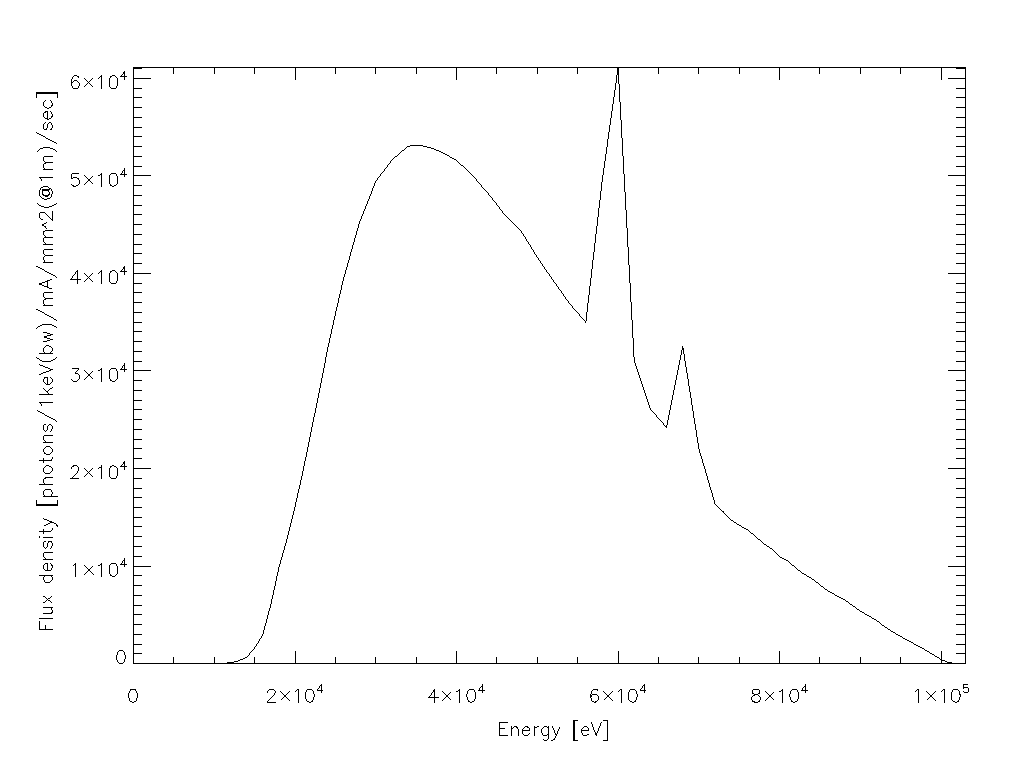
\includegraphics[%width=0.9\textwidth
  height=0.29\textheight]
  {figures/XrayTube/XrayTubeSpec.png}
  \caption[Spectrum of a Tungsten X-ray tube.]{Spectrum of a Tungsten
    X-ray tube operated at $E=\SI{100}{\kilo\eV}$ without filters.
    The two characteristic lines in the spectrum are the $K_\alpha$-
    and $K_\beta$-line of of Tungsten.  They correspond to X-rays
    emitted during the transition of electrons from the L-shell and
    M-shell to the K-shell, respectively.  The fine-structure
    splitting of energy levels, which is indicated by a subindex, is
    not resolved in the plot.  The energies belonging to the mentioned
    transitions are: $K_{\alpha_1}=\SI{59.32}{keV}$,
    $K_{\alpha_2}=\SI{57.99}{keV}$, $K_{\beta_{2}}=\SI{69.10}{keV}$,
    $K_{\beta_{1}}=\SI{67.24}{keV}$, and
    $K_{\beta_{3}}=\SI{66.95}{keV}$ \cite{Henke1993}.  The spectrum
    was calculated using XOP (X-ray Oriented Programs) provided by
    \ac{esrf} \cite{Sanchez2011}.}
  \label{fig:xray-tube-spec}
\end{figure}
%%%%%%%%%%%%%%%%%%%%%%%%%%%%%%%%%%%%%%%%%%%%%%%%%%%%%%%%%%%%%%%%%%%%%%
% Tungsten (Wolfram) W, atomic number Z=74,
%          K-edge  KNIII  KMIII  KMII   KLIII  KLII
%                  Kβ2    Kβ1    Kβ3    Kα1    Kα2
% Inten.           2-5    ~20    ~10    100    50-53    
% Inten.           5–15   ~20    ~10    100    53–65
%          69.517  69.100 67.244 66.951 59.318 57.982 


\subsection{Synchrotron radiation facilities}
\label{sec:synch}

Synchrotron light sources are categorised into three generations.
This number increases to four when \ac{FEL} are included.  First
generation sources refer to accelerators and storage rings which were
primarily meant for experiments in high-energy physics.  Designated to
collide or store particles, synchrotron radiation is an unwanted
by-product of storage rings.  Initially, the radiation was used in
parasitic operation only.  %\eg{} at the EMBL outstation on DESY
For example, one of the first diffraction experiments (on an insect
muscle) was conducted at the German electron synchrotron \acs{DESY}
providing parasitic radiation in the X-ray regime down to sub-angström
wave lengths \cite{Rosenbaum1971,XDB}.
% This opportunity came to the attention of biological
% crystallographers with the report, published in 1971, of at the DESY
% synchrotron in Hamburg
From the beginning in 1974, the double ring storage DORIS (Doppel-Ring
Speicher) at \ac{DESY} was also used as a source of synchrotron
radiation, and by 1993 this was its sole purpose \cite{XDB}.  In X-ray
crystallography synchrotron facilities have become the most important
source of X-rays, for both minerals and organic crystals.  As a
consequence of the large unit cell volume of crystallised biological
macromolecules the diffracting power is weak compared to minerals and
metals.  Moreover, the growth of large crystals of biological
macromolecules is difficult.  Therefore the use of  intense and
brilliant radiation provided by synchrotrons is essential for
structural studies of biological macromolecules \cite{Lindley1995}.
By now, synchrotron facilities have contributed to the structure
determination of tens of thousands of proteins and nucleic acids.  For
instance, the structural determination of the ribosome, which is the
molecular machine that serves as the primary site for protein
synthesis and consists of the large and small ribosomal sub-unit, was
partly done at DORIS \cite{Yonath2000,Yonath2001}.  Second- and
third-generation synchrotrons refer to facilities devoted to the
production of brilliant and intense light only.  While in
second-generation facilities X-rays are produced by bending magnets
which force electrons onto a circular trajectory, third generation
sources exploit periodic arrays of magnets, called \acfp{id}, which
are situated in straight sections of the storage ring.  The
alternating magnetic field in an \acl{id} forces the electrons to move
sinusoidally.  Light emitted at each period adds up to boost the
intensity by up to four orders of magnitude compared to that of a
\acf{bm}.  %, see \cref{fig:undulator}.
The first light source of the third generation type to be built was
the \ac{esrf}, completed in 1991.

The principal layout of the accelerator complex in a synchrotron
radiation facility is composed of a pre-injector, the booster
synchrotron, and the storage ring, see \eg{} \cref{fig:anka}.  The
pre-injector is typically composed of an electron gun, where electrons
are produced by local heating, a bunch compressor, where electrons
are packed in bunches, and a linear accelerator such as a microtron,
where  electrons are accelerated to energies sufficient for
injection into the booster synchrotron.  In the booster synchrotron
the electrons are pre-accelerated before being injected into the
storage ring.  Unless injected at full energy, the beam has to be
ramped up in energy in the storage ring to reach final operating
conditions.  Thus a refill of electrons followed by a ramp-up is
usually required once or twice per day.  In a full energy injector a
booster synchrotron is used whose circumference and energy match that
of the storage ring.  This enables top-up operation to compensate for
beam losses by periodically injecting small amounts of current.  The
aim of the top-up operation mode is to maintain a steady current in
the storage ring to overcome lifetime limitations and to keep a
constant photon flux at the beamline.  A constant flux is not only
important to keep up photon statistics during the measurement, but
also to attain  thermal equilibrium of the heat load on the X-ray
optics, see \cref{fig:flat-thermal-expansion} for the distorting
impact of heat load on a multilayer monochromator.  Typical machine
components of the accelerator complex involve radio frequency cavities
for direct acceleration, dipole magnets (bending magnets) for
deflection of particles, and quadrupole or sextupole magnets for beam
focusing.
% ANKA %%%%%%%%%%%%%%%%%%%%%%%%%%%%%%%%%%%%%%%%%%%%%%%%%%%%%%%%%%%%%%%
\begin{figure}
  \centering
  \includegraphics[width=0.8\textwidth]
  {figures/Synchrotron/SynchrotronLayout-ANKA}
  \caption[Layout of the \ac{anka} synchrotron radiation
  facility.]{Layout of the \ac{anka} synchrotron radiation facility
    including pre-injector (Mikrotron), booster synchrotron
    (\SI{500}{MeV} Booster), and storage ring (\SI{2.5}{GeV}
    Speicherring).  Also shown is the outline of the optics and
    experimental hutches, the radiation shield wall, radio cavities
    (\SI{500}{MHz} RF), and insertion devices (Undulator, Wiggler).
    Image taken from \cite{ANKAInstrBook2012}.}
  \label{fig:anka}
\end{figure}
%%%%%%%%%%%%%%%%%%%%%%%%%%%%%%%%%%%%%%%%%%%%%%%%%%%%%%%%%%%%%%%%%%%%%%

The basic physical properties of synchrotron radiation are determined
by the fact that a charge moves at relativistic velocities towards the
observer.  A non-relativistic electron moving on a circular trajectory
acts similar to a Hertz dipole, isotropically emitting radiation
perpendicular to its axis of acceleration.  In a synchrotron, however,
electrons travel at relativistic speed $\vec{v}$ with their energy
$E_e$ being large compared to the rest energy of $\me
c^2=\SI{511}{keV}$.  This is expressed by the Lorentz factor as
\begin{equation}
  \label{eq:gamma}
  \gamma =\frac{E_e}{\me^2c^2} 
  =\frac{1}{1-\frac{v^2}{c^2}}=\frac{1}{1-\beta^2}\gg1\;,
\end{equation}
where $\beta=v/c$ denotes the modulus of the velocity
$v=\abs{\vec{v}}$ normalised to the speed of light in vacuum $c$, and
$\me$ is the electron rest mass.  As a consequence, the radiation
received by the observer in the laboratory frame is confined in a
light cone centred around the instantaneous velocity of the electron.
The opening angle $\theta$ of the light cone is approximately given
in terms of the Lorentz factor as \cite{Hofmann2004Book}
\begin{equation}
  \label{eq:angle}
  \theta \approx \sin(\theta) = \frac{1}{\gamma}\;.
\end{equation}
The time in the rest frame of the charge during which an observer
receives radiation emitted by that charge is much longer than the time
in the laboratory frame of the observer.  This compression of time
(Doppler effect) is what determines the spectrum of synchrotron
radiation.
% LONG MAGNET %%%%%%%%%%%%%%%%%%%%%%%%%%%%%%%%%%%%%%%%%%%%%%%%%%%%%%%%
\begin{figure}
  \centering
  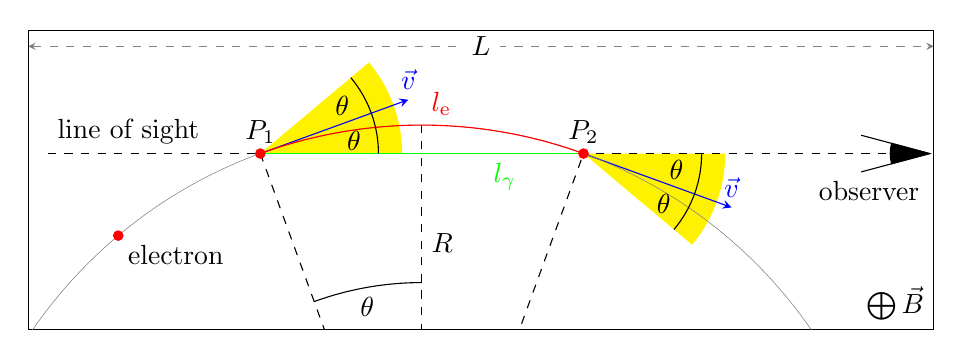
\begin{tikzpicture}[>=stealth]
    % magnet
    \draw[dashed,help lines,<->] (-5,7) --+(5.75,0) 
    node[black,fill=white!100] {$L$} --+(11.5,0);
    \clip[preaction = {draw}] (-5,3.4) rectangle +(11.5,3.8);
    \draw (-5,3.4) +(11.5,0) node[above left] {$\bigoplus\vec{B}$};
    % left: light cone
    \fill[color=yellow,%opacity=0.5
    ] (110:6) node[above,black,%opacity=1
    ]
    {$P_1$} -- +(0:1.8) arc(0:40:1.8) -- cycle;
    % left: velocity
    \draw[blue,->] (110:6) --+(20:2cm) node[above] {$\vec{v}$};
    % right: light cone
    \fill[color=yellow,%opacity=0.5
    ] (70:6) node[above,black,%opacity=1
    ]
    {$P_2$} -- +(0:1.8) arc(0:-40:1.8) -- cycle;
    % right: velocity
    \draw[blue,->] (70:6) -- +(-20:2cm) node[above] {$\vec{v}$};;
    % line of sight
    \draw[dashed] (110:6) +(-2.7,0) 
    node[above right] {line of sight} -- ++(8,0);
    % observer
   \filldraw[] (110:6) ++(8.5,0) --+(165:0.5) arc(165:195:0.5cm) -- cycle;
    \draw[] (110:6) ++(8.5,0) --+(165:0.9);
    \draw[] (110:6) ++(8.5,0) --+(195:0.9);
    \draw[] (110:6) ++(8.6,0) +(195:.9) node[below] {observer};
    % charge trajectory
    \draw[help lines] (180:6) arc (180:0:6);
    % light path
    \draw[green] (70:6) -- (110:6);
    \draw[green] (70:6) +(-1,0) node[below,green] {$l_{\gamma}$};
    % vertical line
    \draw[dashed] (0,0) -- (0,6) node[red,above right] {$l_{\mathrm{e}}$};
    \draw (0,4.5) node[right] {$R$};
    % horizontal arc
    \draw (0,4) arc(90:100:4) node[below] {$\theta$} arc(100:110:4);
    \draw[dashed] (110:6cm) -- (0,0) -- (70:6cm);
    \draw[red] (110:6cm) arc (110:70:6cm) ;
    % left: angle
    \draw[] (110:6) +(0:1.5) arc(0:40:1.5);
    \draw[] (110:6) +(8:1.2) node[] {$\theta$} +(30:1.2) node[] {$\theta$};
    % right: angle
    \draw[] (70:6) +(0:1.5) arc(0:-40:1.5);
    \draw[] (70:6) +(-10:1.2) node[] {$\theta$} +(-32:1.2) node[] {$\theta$};
    % charge
    \filldraw[red](130:6) circle(.06) node[black,below right] {electron} 
    (110:6) circle(.06) (70:6) circle(.06);
  \end{tikzpicture}
  \caption[Radiation emitted in a long magnet.]{Electron moving at a
    velocity $v=\abs{\vec{v}}$ in a long magnet of constant magnetic
    field $B=|\vec{B}|$ and length $L > \frac{2R}{\gamma}=\frac{2
      \me}{e B}$.  Thereby, radiation is emitted into a light cone
    (yellow) with an opening angle $\theta$.  The emitted radiation is
    received by the observer as long as the velocity subtends an angle
    to the line of sight less than the opening angle $\theta$ of the
    radiation cone.  Therefore, the length of the radiation pulse as
    seen by the observer is given by the difference in time for the
    charge and the radiation to travel from  $P_1$ to $P_2$.}
  \label{fig:long-magnet}
\end{figure}
%%%%%%%%%%%%%%%%%%%%%%%%%%%%%%%%%%%%%%%%%%%%%%%%%%%%%%%%%%%%%%%%%%%%%%

Consider a charge which is moving on a circular trajectory with radius
$R$ and velocity $v$ in a constant magnetic field $B$ as depicted in
\cref{fig:long-magnet}.  The radiation emitted by the charge is
received by the observer only as long as the velocity vector of the
charge subtends an angle to the line of sight less than the opening
angle of the radiation cone.  The corresponding locations of the
trajectory are indicated by $P_1$ and $P_2$ in \cref{fig:long-magnet}.
The length of the pulse received by the observer is thus determined by
the difference in time for the charge and the radiation to travel from
$P_1$ to $P_2$.  Hence the pulse length in a long magnet reads from
\cref{fig:long-magnet} as
\begin{equation}
  \label{eq:long-magnet-pulse}
  \Delta t_{\mathrm{lm}} 
  = t_\mathrm{e}-t_\gamma 
  = \frac{l_\mathrm{e}}{v} - \frac{l_\gamma}{c}
  = \frac{2R}{\beta\gamma c}-\frac{2R\sin(1/\gamma)}{c}
  \approx \frac{4R}{3c\gamma^3}\;,
\end{equation}
where an approximation for ultra-relativistic velocities,
$\beta\approx 1$ and $\gamma\gg1$, and an expansion of the
trigonometric function was used.  The radiation obtained from a long
magnet is usually referred to as (ordinary) synchrotron radiation.  It
exhibits a broad spectrum characterised by the critical frequency
$\omega_{\mathrm{crit}}$ which is proportional to the frequency
associated to \cref{eq:long-magnet-pulse}.  Defined such as to halve
the emitted power, the critical frequency is found as
\cite{Hofmann2004Book}
\begin{equation}
  \label{eq:omega-critical}
  \omega_{\mathrm{crit}}=\frac{3 c\gamma^3}{2R}
  = \frac{2}{\Delta t_{\mathrm{lm}}}\;.
\end{equation}

% SHORT MAGNET %%%%%%%%%%%%%%%%%%%%%%%%%%%%%%%%%%%%%%%%%%%%%%%%%%%%%%%
\begin{figure}
  \centering
  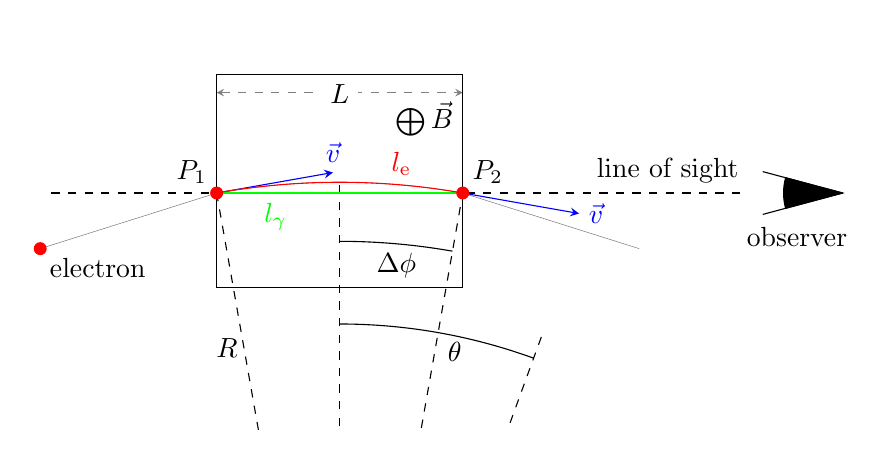
\begin{tikzpicture}[scale=1.5,>=stealth]
    % clipping
    \clip[] (100:6) ++(-1.6,-2) rectangle +(7.1,3.4);    
    % magnetic field box width
    \draw[dashed,help lines,<->] (0,0.85) +(0,5.9) 
    node[black,fill=white!100] {$L$} 
    +(100:6)--+(80:6) node[black,below left] {$\bigoplus\vec{B}$};
    % magnetic field box    
    \draw[yshift=-0.8cm] (100:6) +(0,1.8) -- +(0,0) 
    -- (80:6) -- +(0,1.8) -- cycle;
    % line of sight
    \draw[dashed] (100:6) +(-1.4,0) -- ++(4.5,0) 
    node[above left] {line of sight};
    observer
    \filldraw[] (100:6) ++(5.3,0) --+(165:0.5) arc(165:195:0.5cm) -- cycle;
    \draw[] (100:6) ++(5.3,0) --+(165:0.7);
    \draw[] (100:6) ++(5.3,0) --+(195:0.7);
    \draw[] (100:6) ++(5.3,-.1) +(195:.4) node[below] {observer};
    % vertical line
    \draw[thin, dashed] (0,0) -- (0,6);
    % phi angle
    \draw (90:5.5) arc(90:85:5.5) node[below] {$\Delta\phi$}
    arc(85:80:5.5); \draw[dashed] (100:6) -- (0,0) -- (80:6); \draw
    (100:4.5) node[above left] {$R$};
    % theta angle
    \draw[dashed] (0,0) -- (70:5);
    \draw (90:4.8) arc(90:80:4.8)
    node[below right] {$\theta$} arc(80:70:4.8);
    % left
    \draw[blue,->] (100:6) node[black,above left] {$P_1$} --+(10:1cm) 
    node[above] {$\vec{v}$};
    % right
    \draw[blue,->] (80:6) node[black,above right] {$P_2$} 
    -- +(-10:1cm) node[right] {$\vec{v}$};;
    % charge trajectory
    \draw[help lines] (115:6) -- (100:6) arc (100:80:6) -- (65:6);
    % path: light
    \draw[green] (100:6) -- (80:6);
    \draw[green] (100:6)+(0.5,0) node[below,green] {$l_{\gamma}$};
    % path: electron
    \draw[red] (100:6) arc(100:80:6)
    (85:6) node[red,above] {$l_{\mathrm{e}}$};
    % charge
    \filldraw[red](115:6) circle(.05) node[black,below right] {electron}
    (100:6) circle(.05) (80:6) circle(.05);
  \end{tikzpicture}
  \caption[Radiation emitted in a short magnet.]{Electron moving at a
    velocity $v=\abs{\vec{v}}$ in a short and weak magnet of constant
    magnetic field $B=|\vec{B}|$ and of length $L <
    \frac{2R}{\gamma}=\frac{2 \me}{e B}$.  The deflection angle
    $\Delta \phi$ is less than the opening angle of the radiation cone
    $\theta$. Thus, the length of the radiation pulse $\Delta
    t_{\mathrm{sm}}$, given by the difference in time for the charge
    and the radiation to travel from point $P_1$ to $P_2$, becomes a
    function of $L$.}
  \label{fig:short-magnet}
\end{figure}
%%%%%%%%%%%%%%%%%%%%%%%%%%%%%%%%%%%%%%%%%%%%%%%%%%%%%%%%%%%%%%%%%%%%%%
Consider a charged particle moving in a short and weak magnet of
length $L$ and constant magnetic field $B$ as depicted in
\cref{fig:short-magnet}.  For $L < \frac{2R}{\gamma}=\frac{2
  \me}{e B}$ an electron is deflected by an angle
\begin{equation}
  \label{eq:short-magnet-angle}
  2 \Delta\phi
  =2\arcsin\left(\frac{L}{2R}\right)
  \approx\frac{L}{R}<\frac{1}{\gamma}\;,
\end{equation}
which is less than the opening angle of the radiation cone. Then, the
length of the radiation pulse becomes proportional to the length of
the magnet.  In the ultra-relativistic case $\beta\approx 1$, we have
\begin{equation}
  \label{eq:short-magnet-pulse}
  \Delta t_{\mathrm{sm}} = t_{\mathrm{e}}-t_\gamma = 
  \frac{2R}{\beta c} \arcsin\left(\frac{L}{2R}\right) -\frac{L}{c}
  \approx\frac{L}{\beta c}(1-\beta)
  \approx\frac{L}{2c\gamma^2}\;.
\end{equation}
The radiation obtained from a series of short and weak magnets is thus
distinguished from ordinary synchrotron radiation.  Insertion devices
are composed of an array of short magnets where electrons move on an
oscillatory path within the radiation cone.  Interference effects may
become important depending on the strength of the magnetic field which
influences amplitude and deflection angle of the electron trajectory
in an insertion device.  This is parametrised by the deflection or
undulator parameter $K$.  It is defined by the ratio of the maximum
deflection angle $\Delta \phi$ of an electron moving in a periodic
magnetic field to the opening angle $1/\gamma$ of the emitted
radiation. If the deflection angle is expressed by the magnetic field,
the undulator parameter reads as
\begin{equation}
  \label{eq:defl}
   K= \frac{\Delta \phi}{1/\gamma}
   =\frac{e B_0\lambda_{\mathrm{u}}}{2\pi \me c}\;,
\end{equation}
where $B_0$ is the peak magnetic field in the insertion device, $e$
the electron charge, and $\lambda_{\mathrm{u}}$
% =\frac{2\pi}{k_{\mathrm{ID}}}$
the period length of the insertion device. For a particular insertion
device called wiggler ($K\gg 1$) the radiation emitted from different
parts along the electron trajectory adds up incoherently and thus
interference effects are insignificant.
% For an undulator one has $K\lesssim 1$, and at harmonics of the
% fundamental frequency $\omega_0$.
In the case of a weak undulator ($K < 1$), the radiation from
different periods adds up coherently producing quasimonochromatic
peaks in the emission spectrum.  These peaks correspond to the
harmonics of the fundamental frequency $\omega_0$ given as
\begin{equation}
  \label{eq:undulator}
   \omega_0 = \frac{2\pi}{\lambda_\mathrm{u}}
   \frac{c\gamma^2}{1+\frac{K^2}{2}+\gamma^2\theta^2} \;,
%  \lambda_m=\frac{\lambda_\mathrm{u}}{2m\gamma^2}(1+\frac{K^2}{2}+\theta^2\gamma^2)\;,
\end{equation}
where $\theta$ denotes the observation angle with respect to the
undulator axis.  Given typical parameters found at synchrotrons,
\cref{eq:undulator} implies that centimetre periods
($\lambda_{\mathrm{u}}$) of the undulator translate into nanometre
wavelengths $\lambda_0=\frac{2\pi c}{\omega}$.  For $K\ll1$ and
on-axis observation ($\theta=0$) the result of
\cref{eq:long-magnet-pulse} is restored with $L=\lambda_{\mathrm{u}}$.
In a strong undulator ($K > 1$) the spectrum is more complicated
containing many harmonics.

A detailed treatment of synchrotron radiation on the basis of retarded
electromagnetic potentials, the Liénard-Wiechert potentials, is
given in \cite{Kim1989} or \cite{Hofmann2004Book} and references
therein.

\subsection{Free-electron laser}
\label{sec:fel}

In a \acf{FEL}, or its much more powerful successor the \ac{XFEL} in
terms of energy radiated per unit time and area, a bunch of electrons
is accelerated to relativistic energies (in the order of \SI{10}{GeV})
by a linear array of normal or superconducting resonators.  The
electrons then undulate through a periodic arrangement of magnets,
thereby generating laser light of extreme
intensity. %see \cref{fig:undulator}.
Compared to common synchrotron undulators, the light generated in the
undulator of a free-electron laser interacts with the undulating
electron significantly.  In a process called microbunching, electrons
are accelerated or decelerated and gradually organise themselves into
a multitude of thin disks by ponderomotive forces \cite{Krapchev1979}.
In contrast to conventional undulators, the radiation is now emitted
synchronously by the microbunched electrons and adds up coherently.
This mechanism is known as \ac{sase} \cite{Andruszkow2000}:
spontaneous emission from initial shot noise in the electron beam is
further amplified by the interaction of the emitted light with the
electron bunch over the full length of the magnetic undulator.  This
results in extremely short pulses of \SIrange{e1}{e2}{fs} duration
(\SIrange{e1}{e5}{flashes/s}), a high degree of coherence, and intense
light with a peak and average brightness of
\begin{equation}
  \label{eq:fel-brightness}
  \begin{split}
    B_{\mathrm{peak}} & \approx 
    \frac{\numrange{e29}{e33}\si{.photons}}
    {\si{s.mm^2.mrad^2.}\SI{0.1}{\percent.bandwidth}} \;,
    \\ B_{\mathrm{average}} &\approx 
    \frac{\numrange{e17}{e25}\si{.photons}}
    {\si{s.mm^2.mrad^2.}\SI{0.1}{\percent.bandwidth}}.
  \end{split}%per-mode = fraction
\end{equation}
Note that starting up from noise results in poor temporal coherence
and a broad and noisy spectrum.  To overcome these deficiencies an
external signal can be used to initiate the process of amplification.
This not only improves monochromaticity, but allows to increase the
photon flux by a highly efficient undulator field taper.  Since
external seeding at angström-scale wavelengths is difficult, self
seeding was first proposed for soft X-rays, and successfully applied
for soft and hard X-rays \cite{Amann2012}.  The idea is to use X-rays
from the first half of the undulator to seed the second half.

The extremely intense flashes of light emitted by an \ac{XFEL} allow
to study tiny structures down to the atomic scale, ultrafast processes
such as the formation or dissociation of molecules, or extreme states
or conditions of pressure and temperature as found deep inside a star.
This comes at the expense of the destruction of the sample by the
radiation delivered by \acp{FEL} and \acp{XFEL}.   At femtosecond
timescale, however, the unfolding of a molecular explosion is slow
enough (roughly \SI{10}{fs}), that X-ray photons, which are not
absorbed within the sample, can scatter off the atoms of the
crystalline structure before thermalisation of the unit cells occurs
and thus give rise to an unadulterated diffraction pattern
\cite{Neutze2000,Chapman2011}.  This is also called diffraction before
destruction.

%%%%%%%%%%%%%%%%%%%%%%%%%%%%%%%%%%%%%%%%%%%%%%%%%%%%%%%%%%%%%%%%%%%%%%
%%%%%%%%%%%%%%%%%%%%%%%%%%%%%%%%%%%%%%%%%%%%%%%%%%%%%%%%%%%%%%%%%%%%%%


\section{Monochromator}
\label{sec:optics}

%%%%%%%%%%%%%%%%%%%%%%%%%%%%%%%%%%%%%%%%%%%%%%%%%%%%%%%%%%%%%%%%%%%%%%
\begin{figure}
  \centering
  \small
 \subfloat[Input phase map.]{\label{lena}
   \includegraphics*[width=.4\textwidth]{figures/QuasiInt/lena.png}}
  \hfill
  \subfloat[Normalised difference map.]{\label{diff}
    \includegraphics*[width=.4\textwidth]
    {figures/QuasiInt/Diff_IntMono_IntPoly.png}}  \hfill
  \subfloat[\%]{\label{diff-scale}
      \psfragfig[height=0.4\textwidth]
      {figures/QuasiInt/Diff_Colorbar}{
        \small
        \psfrag{0.1}{0.1}\psfrag{0.2}{0.2}\psfrag{0.3}{0.3}
        \psfrag{0.4}{0.4}\psfrag{0.5}{0.5}\psfrag{0.6}{0.6}
        \psfrag{0.7}{0.7}\psfrag{0.8}{0.8}\psfrag{0.9}{0.9}
        \psfrag{1}{1.0}\psfrag{1.1}{1.1}\psfrag{1.2}{1.2}
        \psfrag{1.4}{1.4}}}  
\\  \subfloat[Monochromatic intensity.]{\label{mono}
    \includegraphics*[width=.4\textwidth]
    {figures/QuasiInt/IntMono.png}}
  \hfill
  \subfloat[Quasimonochromatic intensity.]{\label{quasi}
    \includegraphics*[width=.4\textwidth]
    {figures/QuasiInt/IntPoly.png}}\hfill
  \subfloat[]{\label{int-scale}
      \psfragfig[height=0.4\textwidth]
      {figures/QuasiInt/Int_Colorbar}{
        \small
        \psfrag{0.9}{}\psfrag{0.92}{0.92}\psfrag{0.94}{}
        \psfrag{0.96}{0.96}
        \psfrag{0.98}{}\psfrag{1}{1.00}\psfrag{1.02}{}
        \psfrag{1.04}{1.04}\psfrag{1.06}{}\psfrag{1.08}{1.08}
      }}
    \caption[Comparison of monochromatic and quasimonochromatic
    propagated intensities.]{Comparison of monochromatic and
      quasimonochromatic intensities in simulated forward propagation
      of an exit wave in Fresnel theory. \subref{lena} Lena test
      pattern with 500 $\times$ 500 pixels is used as pure-phase
      object.  The maximum phase variation $\Delta\phi$ over the
      entire field of view is $\Delta\phi= \num{0.1}$ at an energy
      $E=\SI{20}{keV}$, a pixel size $\Delta x = \SI{1}{\micro\metre}$,
      and a propagation distance $z=\SI{1}{m}$.  \subref{mono}
      Intensity $I_{\mathrm{mono}}$ due to a monochromatic spectrum at
      $E=\SI{20}{keV}$.  \subref{quasi} Intensity $I_{\mathrm{quasi}}$
      due to a quasimonochromatic spectrum which is modelled using a
      Gaussian distribution with a mean energy $\avg{E}=\SI{20}{keV}$
      and a bandwidth \num{e-1}.  The corresponding \acf{fwhm} is
      $\Delta E=\SI{2}{keV}$ or a standard deviation of $\sigma =
      \Delta E/(2\sqrt{2\ln(2)})\approx\SI{0.85}{keV}$.  The spectrum
      is sampled at 500 points within an energy range of $\avg{E}\pm
      5\sigma$.  The quasimonochromatic intensity pattern is obtained
      using the Gaussian weighted sum of monochromatic intensities
      computed from phase maps where $\Delta\phi$ varies with energy
      according to the real part of the refractive index
      \cite{Henke1993} $\delta$ and with $\Delta\phi=0.1$ at
      $E=\SI{20}{keV}$.  Within $\avg{E}\mp 5\sigma$, $\Delta\phi$
      decreases from \numrange{1.61}{0.68}.  \subref{diff} Difference
      between the monochromatic and quasimonochromatic intensity
      normalised to the monochromatic intensity
      $|I_{\mathrm{quasi}}-I_{\mathrm{mono}}|/I_{\mathrm{mono}}$.  At
      a broad bandwidth of \num{e-1} the deviations due to a
      quasimonochromatic spectrum are in the order of \SI{1}{\percent}
      only, which is comparable to or less than the typical noise
      level in a measured intensity map.  This simulation, however,
      does not account for the effects of finite transverse and
      longitudinal coherence lengths.  With regard to high-resolution
      phase retrieval, the longitudinal coherence
      (\cref{eq:quasi-mono-coherence-limit})) imposes a more severe
      bound on monochromaticity than that could be inferred from this
      simulation.  \subref{diff-scale} Grayscale to
      \subref{diff}. \subref{int-scale} Grayscale to \subref{mono} and
      \subref{quasi} for normalised intensity maps %$I_z / \Iin$.
}
  \label{fig:quasimono-int}
\end{figure}  
%%%%%%%%%%%%%%%%%%%%%%%%%%%%%%%%%%%%%%%%%%%%%%%%%%%%%%%%%%%%%%%%%%%%%%


%%%%%%%%%%%%%%%%%%%%%%%%%%%%%%%%%%%%%%%%%%%%%%%%%%%%%%%%%%%%%%%%%%%%%%
\begin{figure}
  \centering
  \includegraphics[width=.5\textwidth]
  {figures/FlatField/Fig01_16-bit.png}
  \caption[Flat field from a multilayer monochromator.]{Flat field
    image showing a horizontal stripe pattern which typically occurs
    in synchrotron X-ray beams subject to a multilayer monochromator.
    Depending on the exposure time, a temporal variation of the
    position of the horizontal stripes can be observed.  This is due
    to cooling-induced thermal instabilities of the multilayer
    monochromator.  Image was recorded at bending magnet beamline
    station 2-BM-B of \ac{aps} at Argonne National Laboratory. A
    quasimonochromatic X-ray beam of energy $E = \SI{30}{keV}$ with a
    bandwidth of $\Delta E/E \approx \num{e-2}$ used.}
  \label{fig:flat-field}
\end{figure}
%%%%%%%%%%%%%%%%%%%%%%%%%%%%%%%%%%%%%%%%%%%%%%%%%%%%%%%%%%%%%%%%%%%%%%

The experimental setup for propagation-based phase contrast does not
require additional optical components with the exception of a
monochromator, unless single\hyph line harmonics of appropriate
bandwidth are available at undulator beamlines.
% light-microscopic objective in the case X-rays are converted to
% visible photons in a scintillator.
When the full energy spectrum of the X-ray beam is used, the only
appreciable phase contrast is due to the enhancement of edges of the
projected object.  Higher\hyph order fringes in the propagated
intensity are smeared out due to the superposition of different
monochromatic components.  Moreover, intensity contrast is dominated
by low\hyph energy components which produce broader fringes (see also
\cref{fig:fringe-evolution}) and are more pronounced due to larger
phase shifts at low energies.  The only phase retrieval to be
performed on such data is the inversion of the Laplacian, which mainly
acts as a low-pass filter suppressing high spatial frequencies and
thus noise.  Using a white spectrum, only a mean phase can be
retrieved due to the superposition of monochromatic components.  Thus,
neither a quantitative result nor a high spatial resolution can be
obtained.  For quantitative and high-resolution phase retrieval
methods to work requires a bandwidth of about \num{e-2} or less,
depending strongly on experimental parameters. This result derives
from empirical values, the simulation presented in
\cref{fig:quasimono-int}, and \cref{sec:coherence}.  In this
simulation a monochromatic intensity map is compared to a
quasimonochromatic intensity map with a considerable bandwidth of
\num{e-1}.  The absolute difference between the two maps is found to
be $\sim\SI{1}{\percent}$, which is comparable or less than the
typical noise in a measured intensity map.  A more severe constraint,
however, is imposed by the finite longitudinal coherence length, see
\cref{eq:quasi-mono-coherence-limit}.
% At such parameters, standard phase retrieval methods are already
% affected by non-linear propagation effects
% introducing artifact in the retrieved phase or by blurring due to
% the finite source size.
Hence, in  propagation-based phase-contrast experiments we can work
with a crystal or multilayer monochromator resulting in a bandwidth in
the order of \num{e-2} or \num{e-4}, respectively.  If radiation
damage, induced by the absorbed dose, is insignificant multilayer are
preferred due to the higher flux density while a sufficient degree of
monochromaticity is retained.  The gain in flux density, however,
comes at the expense of an inhomogeneous background field (flat
field).  Typical artifacts in the reflected wave front introduced by a
multilayer are background modulations in terms of an irregular, stripe
pattern \cite{Rack2010,Dietsch2011,Moosmann2013nature}, see \eg{}
\cref{fig:flat-field} and \cref{fig:flat-thermal-expansion} or images
in reference \cite{Rack2010}.  Variations in the surface texture of
the substrate underlying the multilayer coating are reproduced by the
multilayer coating.  These variations result in a different path
lengths introducing phase shifts in the reflected wave front.  By
free\hyph space propagation of the reflected beam, these phase shifts
translate into intensity modulation downstream of the multilayer.  The
stripe pattern is thus influenced by the roughness and composition of
the multilayer \cite{Dietsch2011,Rack2010}.
%%%%%%%%%%%%%%%%%%%%%%%%%%%%%%%%%%%%%%%%%%%%%%%%%%%%%%%%%%%%%%%%%%%%%%
\begin{figure}
  \centering
  \includegraphics*[width=.5\textwidth]
  {figures/FlatField_ThermalExpansion/FlatField_ThermalExpansion.png}
  \caption[Heat load induced flat-field modulations.]{Heat load
    induced thermal expansion of the multilayer affecting stripe-like
    modulations in the flat field.  The left and right half of the
    image depict flat fields which were taken with a delay of
    $\sim\SI{13}{min}$.  The inset at the upper right is an enlarged
    view of the encircled region in the lower half.  Due to thermal
    expansion of the multilayer the stripe pattern becomes magnified
    and shifted.  Data was recorded with beamline ID19 at \ac{esrf}
    using a single multilayer monochromator at \SI{30}{keV}.}
  \label{fig:flat-thermal-expansion}
\end{figure}
%%%%%%%%%%%%%%%%%%%%%%%%%%%%%%%%%%%%%%%%%%%%%%%%%%%%%%%%%%%%%%%%%%%%%%
This is aggravating the flat-field correction procedure and introduces
artifacts in the reconstructed images or tomographic volumes.
Moreover, heat load on the multilayer results in thermal expansion and
instabilities which causes the stripe modulations to vary with time.
While thermal expansion induces  enlargement and shift of the stripe
pattern as seen in \cref{fig:flat-thermal-expansion}, thermal
instabilities, \eg{} introduced by the cooling system of the
monochromator, induce oscillations of the stripe pattern if the
exposure time is smaller than the inverse frequency of the
oscillations.

%%%%%%%%%%%%%%%%%%%%%%%%%%%%%%%%%%%%%%%%%%%%%%%%%%%%%%%%%%%%%%%%%%%%%%
%%%%%%%%%%%%%%%%%%%%%%%%%%%%%%%%%%%%%%%%%%%%%%%%%%%%%%%%%%%%%%%%%%%%%%


\section{Detector system}
\label{sec:detector}

%%%%%%%%%%%%%%%%%%%%%%%%%%%%%%%%%%%%%%%%%%%%%%%%%%%%%%%%%%%%%%%%%%%%%%
\begin{figure}
  \centering
  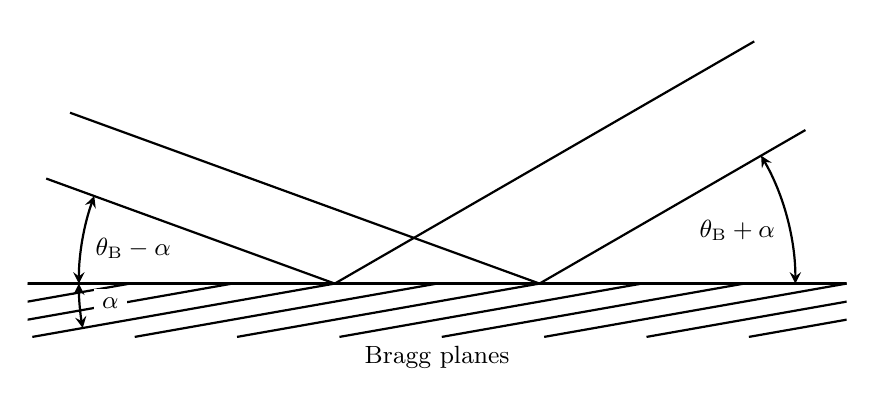
\begin{tikzpicture}[scale=1.3,>=stealth,thick]
    \small
    \clip[] (-1-3,-1) rectangle (1+3,2.5);
    \foreach \beta in {20}
    {
    \foreach \alp in {10}
    { 
      % Bragg planes
      \draw[] (-5,0) -- (5,0); 
      \foreach \x in {-5,-4,...,8} 
      { 
        \draw[] (\x,0)-- +(180+\alp:3);
      }
      \draw (0,-{3*sin(\alp)}) node[below] {Bragg planes};
      % reflex
      \foreach \len in {3}
      {
        \draw[] (-1,0)+(180-\beta:\len+0)--+(0,0)
        --+(\alp+\beta:\len+0.866*2);
        \draw[] (1,0)+(180-\beta:\len+0.94*2)--+(0,0)
        --+(\alp+\beta:\len);
      }
     % angles
     % alpha
      \draw[<->] (-1-2.5,0) arc(180:180+\alp:2.5);
      \draw[] (-1,0) +(180+\alp/2:2.2) node[fill=white!100] 
      {$\alpha$};
      % bragg -alpha
      \draw[<->] (-1-2.5,0) arc(180:180-\beta:2.5);
      \draw[] (-1,0) +(180-\beta/2:2) node[] 
      {$\theta_{\mathrm{B}}-\alpha$};
      % bragg +alpha
      \draw[<->] (1+2.5,0) arc(0:\alp+\beta:2.5);
      \draw[] (1,0) +(\alp/2+\beta/2:2) node[] 
      {$\theta_{\mathrm{B}}+\alpha$};}  }
  \end{tikzpicture}
  \caption[Asymmetric one-dimensional Bragg diffraction in a Bragg
  magnifier.]{Asymmetric one-dimensional Bragg diffraction. The Bragg
    planes subtend an angle $\alpha$ to the surface of reflection.
    $\theta_{\mathrm{B}}$ denotes the Bragg angle.  The incident and
    reflected wave subtend an angle $\theta_{\mathrm{B}}-\alpha$ and
    $\theta_{\mathrm{B}}+\alpha$ with respect to the surface.  The
    magnification factor is $M =
    \frac{\sin(\theta_{\mathrm{B}}+\alpha)}{\sin(\theta_{\mathrm{B}}-\alpha)}$.}
  \label{fig:bragg-magnifier}
\end{figure}
%%%%%%%%%%%%%%%%%%%%%%%%%%%%%%%%%%%%%%%%%%%%%%%%%%%%%%%%%%%%%%%%%%%%%%

To fully exploit the intense radiation available at synchrotron
beamline requires not only fast detectors with a spatial resolution in
the micrometre or submicrometre regime, but also an online data
acquisition.  This enables tomography and time-resolved experiments
and facilitates selection, processing, and distribution of acquired
images.

Using photographic films for X-ray detection achieves micron
resolution for hard X-rays, but is slow, off-line, and has a low
dynamic range \cite{Koch1998}.  Photoresists achieve submicrometre
resolution, but only for soft X-rays, and only work off-line
\cite{Koch1998}.  Therefore image acquisition with a digital sensor
such as a \ac{ccd} or a \ac{cmos} is preferred with the further
benefit of excellent linearity, high stability, a large dynamic range,
and image readout a few milliseconds after exposure \cite{Tate1997}.
Limiting factors of digital cameras in direct detection mode are pixel
sizes (currently in the order of a few microns), radiation damage, and
X-ray stopping power.  Luminescent screens are employed to increase
the stopping power.  For instance, phosphor screens can be used which
consist of a fine grain powder deposited on a substrate
\cite{Gruner2002}.  Multiple photon scattering at the granular
structure of the phosphor screen degrades spatial resolution.  This
can be mitigated by the use of structured scintillators
\cite{Martin2006}.

Another means to improve spatial resolution is the Bragg magnifier
system consisting of a pair of asymmetric cut crystals.  The cross
section of the X-ray beam is increased by asymmetric Bragg reflection
yielding a magnification of up to two orders of magnitude
\cite{Stampanoni2002,Schaefer2003}, see \cref{fig:bragg-magnifier}.
Avoiding the conversion of X-rays into visible light, this setup
facilitates the use of directly converting detectors to achieve
submicron spatial resolution imaging while a high detection efficiency
is maintained.

%%%%%%%%%%%%%%%%%%%%%%%%%%%%%%%%%%%%%%%%%%%%%%%%%%%%%%%%%%%%%%%%%%%%%%
\begin{figure}
  \centering
  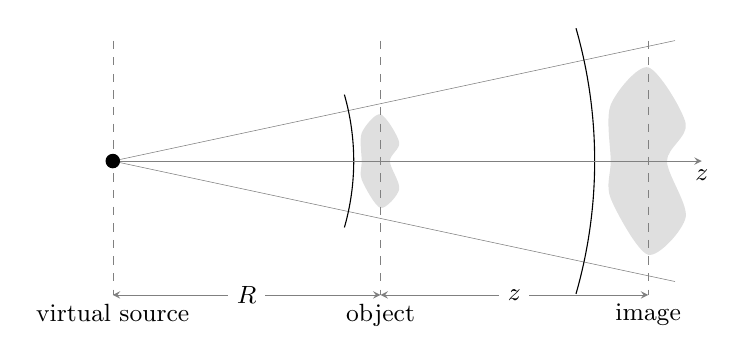
\begin{tikzpicture}[scale=1.7,>=stealth]
    \small
    % Parameters
    \def\zposo{2cm};\def\zposi{4cm};\def\yposh{-1cm};\def\yy{0.9cm};
    \def\arcz{1.8cm};
    % vertical line at zero
    \draw[dashed,help lines] (0,\yy)--(0,\yposh)
    node[below,black]{virtual source};
    % rays
    \draw[black,help lines](0,0)--(\zposi+0.2cm,\yy);
    \draw[black,help lines](0,0)--(\zposi+0.2cm,-\yy);
    % spherical wave
    \draw (\arcz,0) arc(0:16:\arcz);
    \draw (\arcz,0) arc(0:-16:\arcz);
    \draw (2*\arcz,0) arc(0:16:2*\arcz);
    \draw (2*\arcz,0) arc(0:-16:2*\arcz);
    % 
    \begin{scope}[xshift=\zposo,scale=0.7]
    \fill[color=gray!25,%opacity=1
    ] plot [smooth cycle] coordinates
    {(-0.2,0) (-0.2,0.3) (0,0.5) (0.2,0.2) (0.1,0) (0.2,-0.3) (0,-0.5)
      (-0.2,-0.2) };
    \end{scope}
    \draw[dashed,help lines] (\zposo,\yy) -- (\zposo,\yposh)
    node[below,black]{object};
    % image
    \begin{scope}[xshift=\zposi,scale={0.7*(\zposi)/\zposo)}]
    \fill[color=gray!25,%opacity=1
    ] plot [smooth cycle] coordinates
    {(-0.2,0) (-0.2,0.3) (0,0.5) (0.2,0.2) (0.1,0) (0.2,-0.3) (0,-0.5)
      (-0.2,-0.2) };
    \end{scope}
    \draw[dashed,help lines] (\zposi,\yy) -- (\zposi,\yposh)
    node[below,black]{image};
    % optical axis
    \draw[->,help lines] (-0,0) -- 
    (\zposi+0.4cm,0)node[black,below]{$z$};
    % point source
    \filldraw[] (0,0)circle(0.05);
    % length
    \draw[<->,help lines] (0,\yposh)--(\zposo,\yposh);
    \draw[] (\zposo/2,\yposh)node[fill=white!100]{$R$};
    \draw[<->,help lines] (\zposo,\yposh)--(\zposi,\yposh);
    \draw[] (\zposi/2+\zposo/2,\yposh)node[fill=white!100]{$z$};
  \end{tikzpicture}
  \caption[Magnification by cone-beam geometry.]{Magnification by
    cone-beam geometry which is due to a (virtual) point source
    emitting spherical waves.  The object is situated at a distance
    $R$ to the source.  At a distance $R+z$ from the source, the image
    of the object is magnified by a factor of $M=\frac{z+R}{R}$.}
  \label{fig:cone-beam-magnification}
\end{figure}
%%%%%%%%%%%%%%%%%%%%%%%%%%%%%%%%%%%%%%%%%%%%%%%%%%%%%%%%%%%%%%%%%%%%%%
Spatial resolutions down to a few nanometres is enabled by hard X-ray
microscopes.  An incoming quasi-parallel beam of X-rays is focused by
a Fresnel zone plate or a pair of Kirkpatrick-Baez mirrors
\cite{Hignette2005} producing a virtual source with a focal spot size
of below \SI{1}{\micro\metre}.  The cone beam geometry of the
transmitted X-rays results in a magnification which increases with
increasing propagation distance, see
\cref{fig:cone-beam-magnification}.  Compared to conventional imaging
beamlines, access to hard X-ray microscopes is rather limited and the
setup is much more restrictive with regard to data acquisition rates
and dose requirements.  Concerning time-resolved or in vivo
experiments only local tomography is feasible.

A detailed comparison of different approaches for fast, dose
efficient, high-resolution detectors is found in \cite{Martin2006} and
references therein.  In the following we restrict our discussion to
indirect detector systems, which are regularly used in X-ray imaging
experiments, see \cref{fig:detector}.  Such a system is comprised of a
luminescent screen (scintillator), a microscope optic, and a digital
camera \cite{Koch1998}.  The scintillator converts absorbed X-ray
photons into visible or ultraviolet light.  The luminescent light is
subsequently magnified by a microscope optic and relayed onto a
digital camera.  The image sensor in digital cameras is usually a
\ac{ccd}, \ac{cmos}, or \ac{tft}.  Assuming \SI{100}{\percent}
transmission of the luminescent light through the microscope optics,
the image formation can be summarised into the following relation for
the number of counts per pixel and second 
\begin{equation}
  \label{eq:photon-counts}
  N = \Phi \cdot \dqe \cdot \adu \;,
\end{equation}
where, as in \cref{eq:bright}, $\Phi$ denotes the spectral flux of
X-ray photons impinging on the detector system, $DQE$ is the detective
quantum efficiency, and $ADU$  the conversion factor of photons
detected within the image sensor to be converted into electrons in the
analog to digital unit.

For a shot-noise limited system and low spatial frequencies, the
detective quantum efficiency, defined as the ratio of the input and
output \acfp{snr} of the detector system, is given as
\cite{Koch1998,Martin2006}
\begin{equation}
  \label{eq:dqe}
  \dqe \equiv \frac{\snr{out}^2}{\snr{in}^2} 
  \approx \eta_{\mathrm{abs}} 
  \lrp{ 1 + \frac{1+\frac{1}{\eta_{v\to e}}}
    {\eta_{\mathrm{coll}}\frac{E}{E_v}\eta_{X\to v} } }  \;.
\end{equation}
The absorption efficiency $\eta_{\mathrm{abs}}$ denotes the fraction
of X-ray photons absorbed within the scintillator as a function of
X-ray energy $E$.  It is given by Beer's law
(\cref{eq:beers-law-2}) as $\eta_{\mathrm{abs}}=1-\exp(-\mu(E)z)$,
$\mu$ being the linear attenuation coefficient of
\cref{eq:linear-attenuation} and $z$ the thickness of the
scintillator.  $\eta_{X\to v}$ denotes the energy conversion
efficiency of X-rays into visible light of energy $E_v$.
% the light yield which is the ability of a scintillating material to
% convert ionising radiation into visible light per unit of absorbed
% energy. Typical values range in the order of tenth of photons per
% keV.  Thus, $E\cdot LY$ gives the number of visible photons emitted
% by the scintillator.
$\eta_{\mathrm{coll}}$ is the collection efficiency of light emitted
from the transparent luminescent screen to be collected by the optical
system.  $\eta_{v\to e}(E_v)$ is the quantum efficiency of the image
sensor for the conversion of visible photons into electrons as a
function of the energy $E_v$ of visible photons.

% Process of scintillation: absorption, conversion, transport. By
% photoelectric effect, Compton scattering, or pair production (for
% very hard X-ray energies), high-energetic (hot) electrons are
% created in the conduction band and holes in the inner-core bands.  A
% cascade of further ionisation processes occur by inelastic
% scattering and Auger effect processes until the electron fall below
% the ionisation threshold.  Then, electrons and holes thermalise by
% the generation of phonons (excitations).  This results in electron
% energies close above the edge of conduction band and holes close
% below the edge of the valence band.

From \cref{fig:detector} the collection efficiency of the objective
follows as
\begin{equation}
  \label{eq:collection-efficiency}
  \eta_{\mathrm{coll}} = 
  \frac{1}{4\pi}\int_0^{2\pi}\intd
  \varphi\,\int_0^{\theta_{\mathrm{sc}}}\sin\theta
  = \frac12\lrp{1 - \sqrt{\sin^2\theta_\mathrm{sc}} }
  \approx\frac{1}{4}\left(\frac{\NA}{n_{\mathrm{sc}}}\right)^2\;,
\end{equation}
where $\varphi$ is the polar angle with respect to the optical axis,
and $\theta_{\mathrm{sc}}$ the opening angle of the light cone within
the scintillator determined by Snell's law as
\begin{equation}
  \label{eq:snell-law}
  n_{\mathrm{sc}}\sin\theta_{\mathrm{sc}} =
  n_{\mathrm{obj}}\sin\theta_{\mathrm{obj}} = \NA\;.
\end{equation}

Let us now consider the characteristics of the scintillator required
for high-resolution imaging.  The X-ray stopping power (or absorption
efficiency) $\eta_{\mathrm{abs}}$ is maximised by increasing number
density and atomic number.  Radiation hardness is a prerequisite, but
often derogates producibility and image quality (reduced light yield,
increased surface roughness, etc.).  The conversion efficiency
$\eta_{X\to v}$ of absorbed X-rays into visible light should be high.
The spectrum $S_{v}(E_v)$ of emitted photons should match the quantum
efficiency $\eta_{v\to e}$ of the image sensor of the camera which is
described by the spectral matching factor
\begin{equation}
  \label{eq:smf}
  \operatorname{SMF} \equiv 
  \frac{\int\Intd{E_v}\eta_{X\to v}S_{v}(E_v)}
  {\int\Intd{E_v}S_{v}(E_v)} \;.
\end{equation}
Afterglow affects the effective dynamic range at high frame rates of
the detector and needs to be minimised.  Linearity between the flux of
absorbed X-rays and the flux of emitted light is demanded.  The
transmittance of the emitted optical light should be high and the
scattering low.  Technical aspects are also important such as
machinability, non-toxicity, mechanical strength, and
non-hygroscopicity.  Commonly used scintillating films consist of
layers of \eg{} YAG (\chemfig{Y_3Al_5O_{12}}), LAG
(\chemfig{Lu_3Al_5O_{12}}), GGG (\chemfig{Gd_3Ga_5O_{12}}), or LSO
(\chemfig{Lu_2SiO_5}) %(lutetium oxyorthosicilate)
doped with Ce, Eu, or Tb %, \eg{} YAG:Ce, LAG:Eu, GGG:Eu, or LSO:Tb
\cite{Martin2009,Cecilia2011}.  A detailed discussion of the
characteristics of different scintillators is given in
\cite{Martin2006,Martin2009,Cecilia2011}.

%%%%%%%%%%%%%%%%%%%%%%%%%%%%%%%%%%%%%%%%%%%%%%%%%%%%%%%%%%%%%%%%%%%%%%
\begin{figure}
  \centering
  \small
  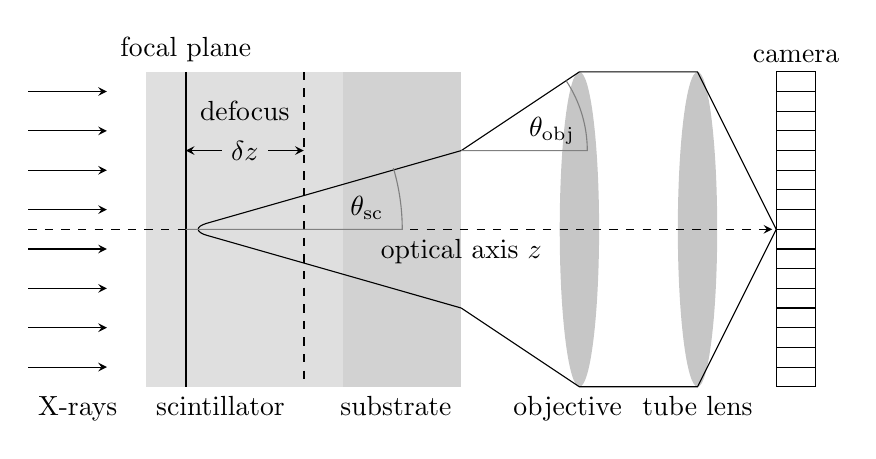
\begin{tikzpicture}[scale=.5,>=stealth]
    % X-rays
  % \clip(-1,-.35)rectangle(1,.35);
    \foreach \y in {-3.5,-2.5,...,3.5}
    { \draw[->] (-1,\y)--(1,\y);}
   \node[below right] at (-1,-4) {X-rays};
   % Substrate
   \fill[xshift=6cm,gray!35] (0,4) rectangle (4,-4) 
   node[below left,black] {substrate};
   % Scintillator
   \begin{scope}[xshift=2cm]
     \fill[gray!25] (0,4) rectangle (5,-4)
     (0,-4) node[below right,black] {scintillator};
     \draw[thick] (1,4) node[above] {focal plane} -- (1,-4);
     \draw[thick,dashed] (4,4) -- (4,-4); 
     \draw[<->] (1,2) -- (4,2);
     \draw (2.5,2) node[fill=gray!25] {$\delta z$} 
     (2.5,3) node[] {defocus};
   \end{scope}
   % Lens
   \fill[xshift=13cm,color=gray!45,%opacity=0.5
   ] (0,0) ellipse (0.5cm and 4cm) 
   (-0.3,-4) node[below,black,%opacity=1
   ] {objective};
   \fill[xshift=16cm,color=gray!45,%opacity=0.5
   ] (0,0) ellipse (0.5cm and 4cm) 
   (0,-4) node[below,black,%opacity=1
   ] {tube lens};
   % Camera
   \draw[xshift=18cm] (0.5,4)node[above,black] {camera};
   \draw[xshift=18cm] (0,-4) grid[xstep=1,ystep=0.5] (1,4);
   % Optical axis
    \draw[->,%opacity=0.8,
    dashed] (-1,0)--(17.9,0);
    \draw[](10,0) node[below,black] {optical axis $z$};
    % light cone
   \begin{scope}[xshift=3cm]
     \draw[rounded corners=8pt] (7,2) -- (0,0) -- (7,-2);
     \draw[] (7,2) -- ++(3,2)--++(3,0)--++(2,-4);
     \draw[] (7,-2) -- ++(3,-2)--++(3,0)--++(2,4);
     \draw[thin,gray] (0,0) -- (5.5,0) arc (0:16.4:5.5cm)
     (4.6,0)node[above,black] {$\theta_{\mathrm{sc}}$};
     \draw[thin,gray] (7,2)--+(3.2,0) arc (0:33.7:3.2cm);
     \draw (9.3,1.9)node[above,black] {$\theta_{\mathrm{obj}}$};
   \end{scope}
  \end{tikzpicture}
  \caption[Indirect detector system involving a scintillator,
  microscope optics, and digital camera.]{Sketch of a detector
    system involving a scintillating screen, microscope optics, and a
    digital camera.  A parallel beam of X-rays impinges
    perpendicularly onto the surface of a luminescent screen
    (scintillator) grown on a substrate.  X-rays that are absorbed
    within the scintillator are converted to visible light which is
    subsequently collected by a microscope objective with numerical
    aperture NA and acceptance angle $\theta_{\mathrm{obj}}$.  Due to
    refraction, the opening angle $\theta_{\mathrm{sc}}$ of the light
    cone within the scintillator is smaller than the acceptance angle.
    The objective is placed such that its front focal plane lies
    within the scintillator.  The magnified light is then imaged on an
    digital camera.  The tube lens, offering the flexibility of
    infinity focus, produces an intermediate image which is either
    directly recorded with a digital camera or further relayed to an
    eyepiece.  An eyepiece produces a real image and offers an
    additional magnification of the intermediate image.}
  \label{fig:detector}
\end{figure}
%%%%%%%%%%%%%%%%%%%%%%%%%%%%%%%%%%%%%%%%%%%%%%%%%%%%%%%%%%%%%%%%%%%%%%

To maximise the intensity signal while maintaining spatial resolution,
it is crucial to understand the interplay of scintillator and
microscope.  Consider a parallel beam setup as depicted in
\cref{fig:detector}, where X-rays impinge perpendicularly onto a
scintillator.  The intensity distribution in the scintillator in
planes perpendicular to the optical axis is assumed to be identical
apart from the attenuation by the absorption of X-rays.  The
intensities of these planes sum up to the total signal recorded by the
camera.  Thus, to acquire a sharp image the objective needs to be
focused at a plane within the scintillator and its depth of focus has
to match the thickness or the absorption length of the scintillator.
The depth of focus (or depth of field) characterises the distance away
from the focal plane where a point object, which is blurred due to
defocusing, still produces a point image.  The resolution limit of a
microscope due to diffraction can only be reached if the thickness or
the absorption length of the scintillator is smaller than the depth of
focus.  %Points out of focus are convoluted with the aperture.
% For a circular aperture the blurred points become circles, and the
% diameter of which where circles are indistinguishable from point
% define the circle of confusion.
Let $R$ denote the resolving power of the microscope, \ie{} the
minimum size of a pattern that can be resolved.  The depth of focus
affects the spatial resolution according to
\cite{Hopkins1955,Koch1998}
\begin{equation}
  \label{eq:dof}
  R \approx \delta z\, \NA\;,
\end{equation}
where $\delta z$ is the distance between the plane in focus and a
plane out of focus, and NA the numerical aperture.  The numerical
aperture is a dimensionless number which characterises the angular
range that a lense can accept.  It is defined as
\begin{equation}
  \label{eq:na}
  \NA = n\sin\theta_{\mathrm{obj}}\;,
\end{equation}
where $\theta_{\mathrm{obj}}$ denotes the half-angle of the
acceptance cone of the lense and $n$ the refractive index of the
medium the lens is immersed in, see \cref{fig:detector}.
% and $M(s)$ is the ratio of the response function of the defocused
% system $D(s)$ to the response function obtained in focus $D_0(s)$.
% The response function (or normalized transmission factor) is given
% by $D(s)=\frac{g(s)}{g(0)}$, where $g(s)$ is the Fourier transform
% of $G=\abs{F}^2$ and $F$ is the Fourier transform of the pupil
% function $f$ with $s$ denoting the one-dimensional, transverse,
% spatial frequency.  Thus $G$ is the diffraction image of a point
% source located in the object plane.  The pupil function takes into
% account the limited acceptance angles of rays, degradational and
% aberrational effect.
The resolving power of a microscope is further limited by diffraction.
Given light of wave length $\lambda$ propagating in a medium of
refractive index $n$, the Abbe diffraction limit for incoherent
illumination (or a self-luminous object) is given by \cite{BornWolf}
\begin{equation}
  \label{eq:diff-limit}
  R\approx \frac12\frac{\lambda}{\NA}\;.
\end{equation}
In geometrical optics, the Abbe diffraction limit can be understood as
follows: the objective lens can be regarded as a device which produces
at the back focal plane a Fourier transformed image of the object in
the front focal plane.  The maximum transverse wave vector that can be
transmitted by the objective is limited by the aperture of the lens to
\begin{equation}
  \begin{split}
    k_{\perp,\mathrm{max}} = \abs{\veck}\sin\theta_{\mathrm{obj}}
    = k\sin\theta_{\mathrm{obj}}
   % = n k_0\sin\theta_{\mathrm{obj}} 
    = \frac{2\pi}{\lambda_0}n\sin\theta_{\mathrm{obj}}
    = \frac{2\pi}{\lambda_0} \NA \;.
  \end{split}
\end{equation}
Using the (two-dimensional) Fourier representation of the object
situated at the front focal plane, the object is decomposed in to
plane waves perpendicular to the optical axis.  Thus the image of the
object transmitted by the lens only contains wave vectors up to
$k_{\perp,\mathrm{max}}$.  The maximum transverse wave vector
associates to the finest detail $R$ that can be resolved as
$k_{\perp,\mathrm{max}}=\frac{2\pi}{2R}$, where the factor of two
takes into account the Nyquist–Shannon sampling theorem
\cite{Nyquist1928,Shannon1949}.  Thus, the diffraction limit 
follows as $R=\frac{\lambda}{2\NA}$.

By matching the resolving powers related to
\cref{eq:dof,eq:diff-limit}, the maximum thickness of the scintillator
in the case of diffraction\hyph limited resolution reads as
\begin{equation}
  \label{eq:dof2}
  \delta z = \frac{\lambda}{2\NA^2}\;.
\end{equation}
The larger the numerical aperture the better the resolving power
according to \cref{eq:diff-limit}.  Moreover, at fixed $n$, a larger
numerical aperture results in a larger angle $\theta_{\mathrm{obj}}$,
which increases the collection efficiency $\eta_{\mathrm{coll}}$ of
the objective.  However, at the same time the depth of focus decreases
according to \cref{eq:dof}.  A smaller depth of focus requires thinner
scintillators decreasing the number of absorbed X-ray photons
($\propto\eta_{\mathrm{abs}}$).  Furthermore, a large numerical
aperture means a short focal length which limits the working distance
of the objective.  The working distance directly influences the
longitudinal extent of the detector system and is defined the distance
between the front end of the objective and its focal plane where the
sample is placed.  It typically decreases with increasing
magnification and numerical aperture.  To protect the camera from
radiation damage, a mirror is usually placed between scintillator and
camera chip.  Using a long working distance objective the mirror can
be placed between scintillator and microscope objective.  This setup
is favourable for high-dose experiments since the objective is
protected from radiation damage.  Objectives with a short working
distance have to be placed before the mirror and are exposed to
X-rays.

% direct single photon counting detector: Medipix, a CMOS pixel
% detector.

% ESRF FReLoN (Fast Readout Low Noise) CCD

% PILATUS(3) CMOS read out, single-photon counting and Hybrid Pixel Technology

% PCO CCD: pco.4000, pco.2000, 

% PCO CMOS: pco.dimax, pco.edge (scientific CMOS)

% PCO edge: IMAGE SENSOR sensor: scientific CMOS (sCMOS), resolution
% (h x v): 2560 x 2160 pixel, pixel size: 6.5 \micron x 6.5 \micron,
% sensor format: 16.6 mm x 14.00 mm, dynamic range: 37000, quantum
% efficienty: >60\%, CAMERA: frame rate: 32fps, exposure/shutter time:
% 500 micro s .. 60 s, dynamic range A/D: 16bit,


% The counts given by the detector often not correspond to the number
% of visible photons.  In principle, the conversion factor can be
% deduced from a set of flat field measurements assuming Poisson
% statistics: the mean values of a fixed pixel over different flat
% fields should be equal to the variance of the same pixel assuming
% Poisson statistics.  If the number of detected visible photons is
% multiplied by a factor $p$, then this factor is given by the ratio
% of variance and mean.  However it has to be taken care of the
% additive noise component caused by the camera dark current inherent
% to the integrating detector system.  \Eg{} in an in vivo experiment
% a typical average count rate is about 4500 photons per pixel with a
% Poisson noise of $1/\sqrt{4500}$.  On the other hand, the mean
% counts due the dark field can be be up to 400 photons per pixel
% corresponding to 8.89\% of noise.  Thus, the conversion factor has
% to be determined from a set of flat field acquired with a very large
% number of counts.




%%%%%%%%%%%%%%%%%%%%%%%%%%%%%%%%%%%%%%%%%%%%%%%%%%%%%%%%%%%%%%%%%%%%%%
%% CHAPTER
%%%%%%%%%%%%%%%%%%%%%%%%%%%%%%%%%%%%%%%%%%%%%%%%%%%%%%%%%%%%%%%%%%%%%%
\chapter{Phase retrieval beyond linearity}
\label{cha:beyond}

% A precursor to the reconstruction of the electron density of the
% object under investigation is the retrieval of the phase map from the
% measured intensity map.  

% !! $\delta \propto \rho_e$ see section...

% Here it is commonly assumed, that the intensity contrast is mainly
% due to phase contrast, \ie{} the sample is considered a pure-phase
% object and absorption is constant, or that the phase-attenuation
% duality assumption holds (see \cref{sec:duality}).  In the following
% we present extensions to standard methods of phase retrieval
% discussed in \cref{sec: linearised version of the \ac{tie} and the
% \ac{ctf} which either employ a perturbation theory approach or the
% concept of quasiparticles.

% For several reasons we are focusing on methods of phase retrieval
% which requires the measurement of single intensity map at a single
% distance only, and are based on intensity contrast emerging by the
% propagation of the exit wave field in free space. In the following
% we will refer to these as single-distance phase retrieval. First of
% all single-distance phase retrieval benefits from its simple
% experimental set up which basically is that of standard absorption
% tomography (or radiography) except for an increased sample to
% detector distance. The usually employed sample-detector distances
% are in the order of tens of centimetres. Compared to multiple
% distance, scanning, or analyser-based techniques its less demanding
% and involves no additional optics than that needed for absorption
% tomography or radiography.  For example, a multiple distance
% technique needs a precise alignment of the stage translating the
% tomography stage with the sample placed atop or a software-based
% realignment of the corresponding intensities at different distances
% after the measurement, or (even) both.  Secondly, when the dose
% deposited in the sample becomes an issue, as it is the case for soft
% tissues or in in vivo imaging, a single-distance, full-field
% approach is obviously favoured over scanning techniques which either
% need to measure a several distances, or need a stepping of a
% grating, or a rocking of an analyser crystal.


%%%%%%%%%%%%%%%%%%%%%%%%%%%%%%%%%%%%%%%%%%%%%%%%%%%%%%%%%%%%%%%%%%%%%%
%%%%%%%%%%%%%%%%%%%%%%%%%%%%%%%%%%%%%%%%%%%%%%%%%%%%%%%%%%%%%%%%%%%%%%

\section{Perturbation theory}
\label{sec:perturbation-theory}

In order to characterise object scales larger than can be achieved
within the edge-enhancement regime, the object-to-detector distance is
increased to values where the intensity pattern contains information
from larger object scales.  This is due to the interference of distant
points in the exit wave field as discussed on the basis of
\cref{eq:guigay} in \cref{sec:ctf}.  At large $z$, however, the linear
model that is assumed in \cref{sec:tie} breaks down and a more general
ansatz is required.  Here we propose and develop a systematic
extension of phase retrieval based on \acf{tie} for pure\hyph phase
objects.  This extension systematically works beyond the linear
approximation of \cref{eq:tie-linear} while maintaining its
single\hyph distance and single\hyph measurement attributes.  In order
to do so we appeal to a model where intensity contrast and phase shift
are expanded in powers of the propagation distance $z$.  Phase
retrieval to leading order (LO) in $z$ restores the result of
linearised \ac{tie} \eqref{eq:linear-tie-phase}.  The expansion
coefficients related to higher orders in $z$ are determined from the
paraxial wave equation \eqref{eq:pwe-2}.  Explicit expressions are
given up to next-to-leading order (NLO) and next-to-next-to-leading
order (NNLO) in terms of transverse derivatives acting on $\phi_0$.
Higher order contributions provide non-linear corrections to the
Laplacian of the phase which are evaluated perturbatively in terms of
the leading-order result.  Such a perturbative approach is well know
and successfully applied in the field of high-energy physics.  We
analyse the extended algorithm on simulated phantom data.  The
discussion presented in the following is adopted from the publications
\cite{Moosmann2010opex,Moosmann2011pssa}.

\subsection{Next-to-leading-order correction}
\label{sec:nlo}

Recall the imaginary (\ac{tie}) and the real part of the paraxial wave
equation given by
\begin{equation}
  \label{eq:pwe-im}
  k\,\pd_z g_z(\vecxp) =
  -\nabla_\perp\left[(g_z(\vecxp)+1)\np\phi_z(\vecxp)\right] \;,
\end{equation}
and
\begin{equation}
  \label{eq:pwe-real}
    2k\pd_z\phi(\vecxp,z)=
  \frac{\np^2\sqrt{g_z(\vecxp)+1}}{\sqrt{g_z(\vecxp)+1}}
  -\left(\np\phi(\vecxp,z)\right)^2 \;,
\end{equation}
respectively. A power-series ansatz for the propagated phase shift
at $z>0$ reads
\begin{equation}
  \label{eq:phase-series}
    \phi_z(\vecxp)=\sum_{l=0}^\lmaxphi\phi\supl(\vecxp)\,z^l \;.
\end{equation}
Accordingly, we make a power-series ansatz for the intensity contrast
\begin{equation}
  \label{eq:g-series}
    g_z(\vecxp)=\sum_{l=1}^\lmaxg g\supl(\vecxp)\,z^l \;.
\end{equation}
Here, $g\supl$ and $\phi\supl$ denote $z$-independent coefficients of
the $z$\hyph dependent functions $g_z$ and $\phi_z$.  Since we assume
a pure-phase object with $g_{z=0}=g\ho0=0$, the summation index in the
ansatz for $g_z$ starts at $l=1$.  To determine the coefficients
$g\supl$ and $\phi\supl$, we substitute ansatz
\cref{eq:phase-series,eq:g-series} into the imaginary part of the
paraxial wave equation \eqref{eq:pwe-im} and sort by powers in $z$.
The resulting equation demands that the sum of coefficients of a given
power in $z$ has to vanish individually to each power in $z$.
Comparing coefficients to lowest order in $z$ yields
\begin{equation}
  \label{eq:g-1}
       g\ho1 = -\frac{1}{k}\np^2\phi\ho0 \;.
\end{equation}
To linear order in $z$ and using \cref{eq:g-1} we have
\begin{equation}
  \label{eq:g-2}
  \begin{split}
     g\ho2 & = -\frac{1}{2k}\,\lrb{ 
       \np g\ho1\cdot\np\phi\ho1 +\np^2\phi\ho1 +g\ho1\np^2\phi\ho0 }
    \\ & = \frac{1}{2k} \lrb{ \frac{1}{k}
      \lrp{ \lrp{\np\np^2\phi\ho0}\cdot\np\phi\ho0  +\lrp
        {\np^2\phi\ho0}^2}
      -\np^2\phi^{(1)} } \,.
  \end{split}
\end{equation}
Coefficients $\phi\ho{l}$ can be computed from 
\cref{eq:phase-series} as
\begin{equation}
  \label{eq:phi-n}
  \phi\ho{l} = \lim_{z\to 0}\frac{1}{l!}\pd_z^l\phi_z 
  \equiv \lim_{z\to 0}\frac{1}{l!}\frac{\pd^l}{\pd z^l}\phi_z \;.
\end{equation}
The coefficient $\phi^{(1)}$ in \cref{eq:g-2} then follows from
\cref{eq:pwe-real,eq:phi-n} in the limit $z\to 0$ as
\begin{equation}
  \label{eq:phi-1}
  \phi\ho1 = \lim_{z\to 0}\pd_z\phi_z = 
  -\frac{1}{2k}\lrp{\np\phi\ho0}^2 \,.
\end{equation}
Setting $\lmaxg=1$ and $\lmaxphi=0$ in
\cref{eq:g-series,eq:phase-series}, respectively, and using
\cref{eq:g-1}, we obtain to linear order in $z$
\begin{equation}
  \label{eq:phase-lo}
  \np^2\phi_{z=0} \equiv \np^2\phi\ho0 = -\frac{k}{z} g_z \;,
\end{equation}
which is the linearised \ac{tie} as in \cref{sec:tie}.  Combining
\cref{eq:phase-series,eq:g-series} truncated at $l_{\mathrm{max},g}=2$
and $l_{\mathrm{max},\phi}=1$ and \cref{eq:g-1,eq:g-2,eq:phi-1}, we
obtain an expression for the Laplacian of the phase to next-to-leading
order as
\begin{equation} 
  \label{eq:phase-nlo}
  \begin{split}
    & \np^2\phi\ho0 = -\frac{k}{z}\,g_z 
    \\ & +\frac{z}{2k}\left[
      \lrp{\np\np^2\phi\ho0}\cdot\np\phi\ho0
      +\lrp{\np^2\phi\ho0}^2 
      +\frac12\np^2\lrp{\np\phi\ho0}^2
    \right] \,. 
  \end{split}
\end{equation}
This result can also be obtained from the Fresnel diffraction integral
assuming constant absorption as it was shown for the lowest\hyph order
result in \cref{sec:tie}, see
\cref{eq:fresnel-propagator-expansion,eq:fresnel-limit-0,eq:fresnel-limit-1}.
The counting in powers of $z$ then is due to the Taylor expansion of
the Fresnel propagator in Fourier space, see
\cref{eq:fresnel-propagator-expansion}.  However, in such a derivation
it is hardly possible to keep track of how non-linear corrections
arise.  This becomes evident if we appeal directly to
\cref{eq:g-1,eq:g-2}: the first two terms in the square bracket arise
from the unpropagated phase while the third term is due to the
propagated phase.  For later use we notice the fact, that the
non-linear correction in \cref{eq:phase-nlo} represents a sum of total
derivatives in $\vecxp$.  The expansion of $\np^2\phi\ho0$ on the
right-hand side of \cref{eq:phase-nlo} can formally be expressed in
powers of derivatives of $\phi\ho0$.  This requires the variation of
$\phi\ho0$ with respect to $\vecxp$ to be weak.  Otherwise the
coefficients of the powers in $z$ become unacceptably large when the
order of the expansion in powers of $z$ is increased.

The exit phase is linked to the data $g_z$ via \cref{eq:phase-nlo}
representing a non-linear partial differential equation for
$\phi\ho0$.  In the following we discuss how to approach a solution to
\cref{eq:phase-nlo}.  In principle, \cref{eq:phase-nlo} could be
solved numerically, subjecting it to appropriate boundary conditions.
Notice that linearised \ac{tie} \eqref{eq:phase-nlo} is invariant
under global shifts of the gradient of the phase
\begin{equation}
  \label{eq:shift-of-grad-phase}
  \np\phi\ho0\to\np\phi'^{(0)} = \np\phi\ho0+\vec{a} \;,
\end{equation}
with $\vec{a}$ being a constant two-dimensional vector, and thus
$\np^2\phi'^{(0)} = \np^2\phi\ho0$.  The presence of additional powers
of $\np\phi\ho0$ in \cref{eq:phase-nlo} as compared to
\cref{eq:phase-lo} clears this ambiguity.

Phase retrieval to leading order is only constrained by \ac{tie},
being the imaginary part of the paraxial wave equation, and represents
Fresnel theory only incompletely.  Expanding beyond leading order also
involves the real part of the paraxial wave equation, and thus
increasingly accounts for the constraints of the full Fresnel theory.
This should also reduce the influence of optical vortices in
$\phi\ho0$ \cite{Gureyev1995,Paganin1998}.

Instead of a brute-force numerical treatment of \cref{eq:phase-nlo} to
find a useful approximation, the right-hand side of
\cref{eq:phase-nlo} can be approached perturbatively in terms of the
leading-order result obtained from \cref{eq:phase-lo}.  This
approximates the non-linear terms in the square bracket in
\cref{eq:phase-nlo}  in terms of the solution $\phi\ho0$ of
\cref{eq:phase-lo}.

A general expression of the right-hand side of \cref{eq:phase-nlo} is
given in terms of the following power series
\begin{equation}
  \label{eq:formal-power-series}
  \np^2\phi\ho0 = \sum_{l=0}^{\lmaxg+1} c\ho{l}(\vecxp) z^l \,.
\end{equation}
In the ideal case, the only coefficient that remains in
\cref{eq:formal-power-series} is $c\ho0$.  \Eg{} when setting
$\lmaxg=2$, as was assumed in the derivation of \cref{eq:phase-nlo},
the term $-\frac{k}{z}\,g_z$ generates a contribution $-k(g\ho1 +g\ho2
z)$.  In the ideal case, the term in the square bracket in
\cref{eq:phase-nlo}, which by definition is linear in $z$, cancels the
linear term arising in $-\frac{k}{z}\,g_z$.  Increasing $\lmaxg=2\to
\lmaxg=3$ the quadratic correction on the right-hand side of
\cref{eq:phase-nnlo} cancels the quadratic term in
$-\frac{k}{z}\,g_z$, and so forth.

Such a counting in powers of $z$ is respected in perturbation theory,
since by the inversion of the Laplacian in a truncation of the
right-hand side of \cref{eq:phase-nlo} at leading order, we yield an
estimate for $\phi\ho0$ which is independent of $z$.  However, this
estimate does not completely cancel the respective powers in $z$ in
the term $-\frac{k}{z}\,g_z$ when substituted in the corrections to
next-to-leading and next-to-next-to-leading order of
\cref{eq:phase-nnlo}.  Nevertheless, the modulus of the coefficients
of these powers is reduced.

Let us now discuss in more detail the next-to-leading-order (NLO)
terms appearing in the square bracket in \cref{eq:phase-nlo}.
Therefore, we introduce following abbreviations
\begin{equation}
  \label{eq:nlo}
  \begin{split}
       \nlo1(\vecxp) &= \lrp{\np\np^2\phi\ho0}\cdot\np\phi\ho0 \;,
    \\ \nlo2(\vecxp) &= \lrp{\np^2\phi\ho0}^2 \;,
    \\ \nlo3(\vecxp) &= \frac12\np^2\lrp{\np\phi\ho0}^2 \;.
  \end{split}
\end{equation}
To leading order we have $g\ho1=\frac{g_z}{z}$.  Thus, in perturbation
theory, the next-to-leading-order terms follow as
\begin{align}
  \label{eq:nlo-1}
  \nlo1(\vecxp) &= k^2 \lrp{\np g\ho1}\cdot\np\lrp{\inp g\ho1} \;,
  \\ \label{eq:nlo-2} 
  \nlo2(\vecxp) &= k^2 (g\ho1)^2 \;,
  \\ \label{eq:nlo-3} 
  \nlo3(\vecxp) &= \frac{k^2}{2}\np^2\lrp{\np\lrp{\inp g\ho1}}^2 \;.
\end{align}
Here, $\inp$ denotes the inverse of the Laplace operator obtained via
the Fourier derivative theorem (\cref{eq:fourier-derivative}),
requiring an appropriate regularisation as in
\cref{eq:inverse-laplacian-regular}.  Up to the factor $\np\phi\ho0$
in $\nlo1$, linking the Laplacian of $\phi\ho0$ to the data $g\ho1$ in
a non-local fashion, the right-hand side of \cref{eq:nlo-1} is local
in $g\ho1$.  Loosely speaking, $\np\phi\ho0$ is obtained by means of a
single integration of the leading-order equation
$\np^2\phi_{z=0}=\np^2\phi\ho0=-\frac{k}{z}\,g_z$.  Furthermore,
$\nlo2$ is completely local in $g\ho1$ while $\nlo3$ is non-local.
Each of the terms $\nlo1$, $\nlo2$, and $\nlo3$ can be decomposed into
a fluctuating and a mean part as
\begin{equation}
  \label{eq:nlo-decomposition}
  \nlo{i}(\vecxp) = 
  \avg{\nlo{i}} +\delta\nlo{i}(\vecxp)\;, \quad i=\{1,2,3\} \;,
\end{equation}
where $\avg{\nlo{i}}$ denotes the average of $\nlo{i}$ over the
\acf{fov} as
\begin{equation}
  \label{eq:mean-value}
  \avg{\nlo{i}} \equiv 
  \frac{  \int_{\fov}\Intdd{\vecxp}\nlo{i}(\vecxp)}
  {\int_{\fov}\Intdd{\vecxp}} \;.
\end{equation}
%  $\avg{\nlo{i}} \equiv \int\Intdd{\vecxp}\nlo{i}(\vecxp)$.
Since $\nlo1+\nlo2$ and $\nlo3$ separately are sums of partial
derivatives, the sum of their means is zero
\begin{equation}
  \label{eq:nlo-mean-sum}
  \sum_{i=1}^3 \avg{\nlo{i}} = 0 \;.
\end{equation}
Because $\nlo3$ is non-local in $g_z$, this term smears $g\ho1$
averaging out large amplitudes.
 
\Cref{eq:nlo-mean-sum,eq:inverse-laplacian-regular-mean}, and the
conservation of average intensity for pure-phase objects in
forward propagation (see \cref{eq:continuity-fresnel}) imply that
\begin{equation}
  \label{eq:g-mean}
  \avg{ g_z}=0 \;.
\end{equation}
From \cref{eq:g-mean} it follows that the phase, retrieved by applying
the regularised inverse Laplace operator $\npa^{-2}$
(\cref{eq:inverse-laplacian-regular}) to the right-hand side of
\cref{eq:phase-nlo}, is of zero mean.  Each of the terms $\avg{\nlo1}$
and $\avg{\nlo2}$ can individually be large but their sum vanishes.
Deviations from this situation can occur by numerical artifacts,
introduced through discrete Fourier transformations, and thus are
subtracted (see also \cref{sec:mean-phase}).  In
\cref{sec:proj-approx} we have expressed the exact phase by a line
integral over the real decrement $\delta_\omega$ of the sample's
refractive index.  Due to $\delta_\omega$ being semi definite, the
exact phase exhibits a non-vanishing mean.  This ambiguity, already
inherent to Fresnel theory (see \cref{eq:intensity-rescaling}),
persists in the perturbative approach: the addition of an arbitrary
constant to the phase
\begin{equation}
  \label{eq:phi-decomposition}
  \phi\ho0(\vecxp) \equiv \avgn{\phi\ho0} + \delta\phi\ho0(\vecxp) \;,
\end{equation}
does not change \cref{eq:phase-nlo} for $\phi\ho0$.  Therefore, when
comparing exact (simulated) with retrieved phase, we subtract the mean
values of which.

Let us now compare the perturbative approach with phase retrieval
based on \ac{ctf}.  In position space and for  pure-phase objects
\ac{ctf} reads
\begin{equation}
  \label{eq:ctf-phase-real-2}
  g_{z}(\vecxp) = 
  -2\left[\sum^\infty_{l=1}\frac{1}{(2 l-1)!}
    \left(\frac{z}{2k}\right)^{2 l-1}
    (\np^2)^{2 l-1}\right]\phi_0(\vecxp) \,.
\end{equation}
The inversion of \cref{eq:ctf-phase-real-2} corresponds to an infinite
summation of powers of $\np^2$ acting on $\phi\ho0$.  Note that the
expansion \cref{eq:g-series} contains these powers of $\np^2$ in a
truncated way, see left-hand side of \cref{eq:phase-nlo} multiplied by
$z$ at order $z$.
% and the term $\propto \nabla^6_\perp\phi_{0;\theta}$ in the sixth
% line of $z\times$ Eq.\,(\ref{cubicnabla^2}) at order $z^3$.
In addition to these terms non-linear corrections in $\phi\ho0$ enter
at these orders.  Therefore, the assumption of weak phase variations
(\cref{eq:weak-phase}) can be increasingly relaxed by taking
increasing powers of $z$ into account in \cref{eq:g-series}.  The
series of \cref{eq:g-series} expands in powers of transverse
derivatives including non-linearities in $\phi\ho0$.  On the contrary,
the expansion in \cref{eq:ctf-phase-real-2} takes into account all
powers of the Laplacian $\np^2$ at linear order in $\phi\ho0$ only.
% For weakly varying phase objects expansion
% \cref{eq:ctf-phase-real-2} is an excellent approximation in treating
% the case where all frequencies contribute to the overall phase shift
% such that the latter is smaller than unity but breaks down as soon
% as a part of the spectrum contributes relative phase shifts
% comparable or larger than unity.
For pragmatic reasons, the non-linear expansion of \cref{eq:g-series}
requires to be truncated at a finite order in $z$.  Thus, large
frequencies are retrieved worse than they are by inverting
\cref{eq:ctf-phase-real-2} within the validity regime of this is
equation.


\subsection{Next-to-next-to-leading-order correction}
\label{sec:nnlo}

% Eq.\,(\ref{tie}) and $l_{\max }-2$ derivatives of
% Eq.\,(\ref{tiereal}) with respect to $z$ are needed to express the
% coefficients in the expansions of Eqs.\,(\ref{ansatzg}) and
% (\ref{ansatzphi}) in terms of polynomials of transverse derivatives
% acting on $\phi\ho0$.

The formal expansion of $\np^2\phi_z$ in powers of $\frac{z}{k}$ can
be carried out to higher orders.  Truncation of ansatz
\cref{eq:phase-series,eq:g-series} at $l_{\mathrm{max},g}=2$ and
$l_{\mathrm{max},\phi}=1$, yields the coefficient of $g_z$ to third
order in $z$
\begin{equation}
  \label{eq:g-3}
  \begin{split}
    g\ho3 = -\frac{1}{3k} &\lb
      \np g\ho1\cdot\np\phi\ho1
      +\np g\ho2\cdot\np\phi\ho0 \right.
      \\ & \left. +\np^2\phi\ho2 
      +g\ho1\np^2\phi\ho1 
      +g\ho2\np^2\phi\ho0 \rb \,.
  \end{split}
\end{equation}
The coefficient of $\phi_z$ to second order in $z$ is obtained from
\cref{eq:pwe-real} and its $z$\hyph derivative in the limit $z\to 0$
as
\begin{equation}
  \label{eq:phase-2}
  \begin{split}
    \phi\ho2 & =\frac{1}{4k} \lrb{ 
      \frac12\np^2 g\ho1 
      -2\np\phi\ho0\cdot\np\phi\ho1 } 
    \\ & = \frac{1}{4k^2}\lrb{
      -\frac12\np^4\phi\ho0 
      +\np\phi\ho0\cdot\np \lrp{\np\phi\ho0}^2 } \,.
  \end{split}
\end{equation}
The Laplacian of the exit phase including the corrections up to
next-to-next-to leading order then reads
\begin{equation}
  \label{eq:phase-nnlo}
  \begin{split}
     & \np^2\phi\ho0 = -\lrp{\frac{z}{k}}^{-1}\,g_z
  \\ &+ \frac12\lrp{\frac{z}{k}} \lrb{ 
    \lrp{\np\np^2\phi\ho0}\cdot\np\phi\ho0 
    +\lrp{\np^2\phi\ho0}^2  \right.
  \\ &\quad\left. +\frac12\np^2\lrp{\np\phi\ho0}^2 }
  \\ &+ \frac{1}{12} \lrp{\frac{z}{k}}^2 \lb
  2\np\lrp{\np^2\phi\ho0}\cdot\np\lrp{\np\phi\ho0}^2 \right.
  \\ &+2\np\phi\ho0\cdot\np\lrp{ \np\phi\ho0\cdot\np\lrp{\np^2\phi\ho0} }
  \\ &+2\np\phi\ho0\cdot\np\lrp{\np^2\phi\ho0}^2
  +\np\phi\ho0\cdot \np\lrp{ \np^2\lrp{\np\phi\ho0}^2 }
  \\ &-\frac12(\np^2)^3\phi\ho0
  +\np^2\lrp{\np\phi\ho0\cdot\np\lrp{\np\phi\ho0}^2 }
  \\ &+3\np^2\phi\ho0\np^2\lrp{\np\phi\ho0}^2
  \\ &+\left. 2\np^2\phi\ho0\np\phi\ho0\cdot\np\lrp{\np^2\phi\ho0}
  +2\lrp{\np^2\phi\ho0}^3 \rb \,.
  \end{split}
\end{equation}


%%%%%%%%%%%%%%%%%%%%%%%%%%%%%%%%%%%%%%%%%%%%%%%%%%%%%%%%%%%%%%%%%%%%%%
\begin{figure}
  \centering
  \begin{tikzpicture}[]
    \def\imsize{0.9\textwidth]}
    \def\yy{0.91\textwidth};
    \def\xxl{-0.2\textwidth};
    \def\xxr{0.15\textwidth};
    \node[anchor=south] at (0,\yy){
      \psfragfig[width=0.9\textwidth]
      {figures/PerturbationTheory/Fig2/Fig2-a} };
    \node[anchor=south] at (0,\yy/2){
      \psfragfig[width=0.9\textwidth]
      {figures/PerturbationTheory/Fig2/Fig2-b} };
    \node[anchor=south] at (0,0){
      \psfragfig[width=0.9\textwidth]
      {figures/PerturbationTheory/Fig2/Fig2-c} };
    \draw[](\xxl,\yy)node[]{(a) $\phi\hon{exact}$};
    \draw[](\xxr,\yy)node[]{(b) $g_z$};
    \draw[](\xxl,\yy/2)node[]{(c) $\phi\hon{LO}$};
    \draw[](\xxr,\yy/2)node[]{(d) $\phi\hon{NLO}$};
    \draw[](\xxl,0)node[]{(e) $\Psi\hon{LO}$};
    \draw[](\xxr,0)node[]{(f) $\Psi\hon{LO+NLO}$};
  \end{tikzpicture}
  \caption[Leading-order phase retrieval and next-to-leading-order
  correction from propagated intensity of a Siemens-star phase
  object. ]{% Modified
    Phase and intensity maps for a Siemens star phase object in
    central projection at a resolution of $2048\times2048$ pixels.
    Mean values were subtracted in all cases. (a) Exact phase map at
    $z=0$.  (b) Map of the intensity contrast at $z=\SI{0.3}{m}$
    generated from the input phase map (a) by Fresnel propagation. (c)
    Leading-order phase $\phi\ho{LO}$ retrieved from intensity map
    (b).  (d) Next-to-leading-order correction $\phi\ho{NLO}$.  (e,f)
    Difference maps $\Psi\ho{NLO}$ and $\Psi\ho{LO+NLO}$, see
    \cref{eq:error-measure} for definition.  Cuts of the phase maps
    presented in \cref{fig:siemens-star-cuts} are taken along the
    green line indicated in (a).  Image adopted with
    modifications from \cite{Moosmann2010opex}.}
  \label{fig:siemens-star}
\end{figure}
%%%%%%%%%%%%%%%%%%%%%%%%%%%%%%%%%%%%%%%%%%%%%%%%%%%%%%%%%%%%%%%%%%%%%%


\subsection{Non-Linear phase retrieval}
\label{sec:perturbation-theory-simulation}

Let us now apply the algorithm for non-linear phase retrieval devised
in \cref{sec:nlo} to simulated data.  A Siemens star pattern is taken
as pure-phase test object.  The ad hoc regularisation of
\cref{eq:inverse-laplacian-regular} is used to invert the Laplacian in
\cref{eq:phase-nlo}, both in the perturbative estimate and the final
expression for $\phi\ho0$.

To characterise the dependence of the retrieved phase on the
regularisation parameter $\alpha$ we define a function $\Phi$ as
follows
\begin{equation}
  \label{eq:phi-alpha}
  \Phi(\alpha) \equiv \sum_{\vecxp}\abs{\phi\ho0(\vecxp)} \;,
\end{equation}
where $\phi\ho0$ is the retrieved phase with a regularisation parameter
 $\alpha$.  The value of $\alpha$ is then chosen such that
$\Phi(\alpha)$ is least sensitive to a variation in $\alpha$.  For the
Siemens-star phantoms considered  we observe $\Phi(\alpha)$ to be
insensitive over a region of several orders of magnitude with a
central value of $\alpha_c\sim 10^{-6}$.

%%%%%%%%%%%%%%%%%%%%%%%%%%%%%%%%%%%%%%%%%%%%%%%%%%%%%%%%%%%%%%%%%%%%%%
\begin{figure}
  \centering
  \tiny
  \begin{tikzpicture}[]
    \def\xx{\textwidth};
    \node[inner sep=0pt,anchor=north] at (0,0){
      \includegraphics[width=0.99\textwidth]
      % [l b r t]%[width=11cm,trim=0cm 0cm 0cm 0cm,clip=true]
  {figures/PerturbationTheory/PT-2-SiemensStarLineCuts}};
 \draw[xshift=0.3cm](-\xx/4,-0.1)node[fill=white!100]{Resolution 512 $\times$ 512}
 (\xx/4,-0.1)node[fill=white!100]{Resolution 2048 $\times$ 2048};
  \end{tikzpicture}
  \caption[Line cuts in leading-order phase retrieval and
  next-to-leading-order correction from propagated intensity of a
  Siemens-star phase object.]{% Modified
    Line cuts through phase maps along the line indicated in
    \cref{fig:siemens-star}(a) for a Siemens star with 32 spokes in
    dependence of propagation distance $z$ (top to bottom) and at two
    distinct resolutions (left to right).  Black lines: exact phase.
    Blue and red lines: phase retrieval referring to leading-order and
    when including next-to-leading-order.  Image adopted with slight
    modifications from \cite{Moosmann2010opex}}
    \label{fig:siemens-star-cuts}
\end{figure}
%%%%%%%%%%%%%%%%%%%%%%%%%%%%%%%%%%%%%%%%%%%%%%%%%%%%%%%%%%%%%%%%%%%%%%

To measure the performance achieved when including the perturbatively
evaluated correction terms in \cref{eq:phase-nlo} compared to the
leading-order linear term, we define the absolute difference map
$\Psi$ as 
\begin{equation}
  \label{eq:error-measure}
  \Psi \equiv \abs{\phi\ho0 -\phi\ho{0,\mathrm{exact}}} \;,
\end{equation}
where $\phi\ho0$ either is the result to leading order (LO) or
including the next-to-leading order (LO + NLO).  A global error
measure is given by $\avg{\Psi}$ defined as the mean of $\Psi$ over
all pixels as in \cref{eq:mean-value}.

%%%%%%%%%%%%%%%%%%%%%%%%%%%%%%%%%%%%%%%%%%%%%%%%%%%%%%%%%%%%%%%%%%%%%%
\begin{figure}
  \centering
  \begin{tikzpicture}[]
    \def\xx{\textwidth};\small
    \node[inner sep=0pt,anchor=south] at (0,0){
      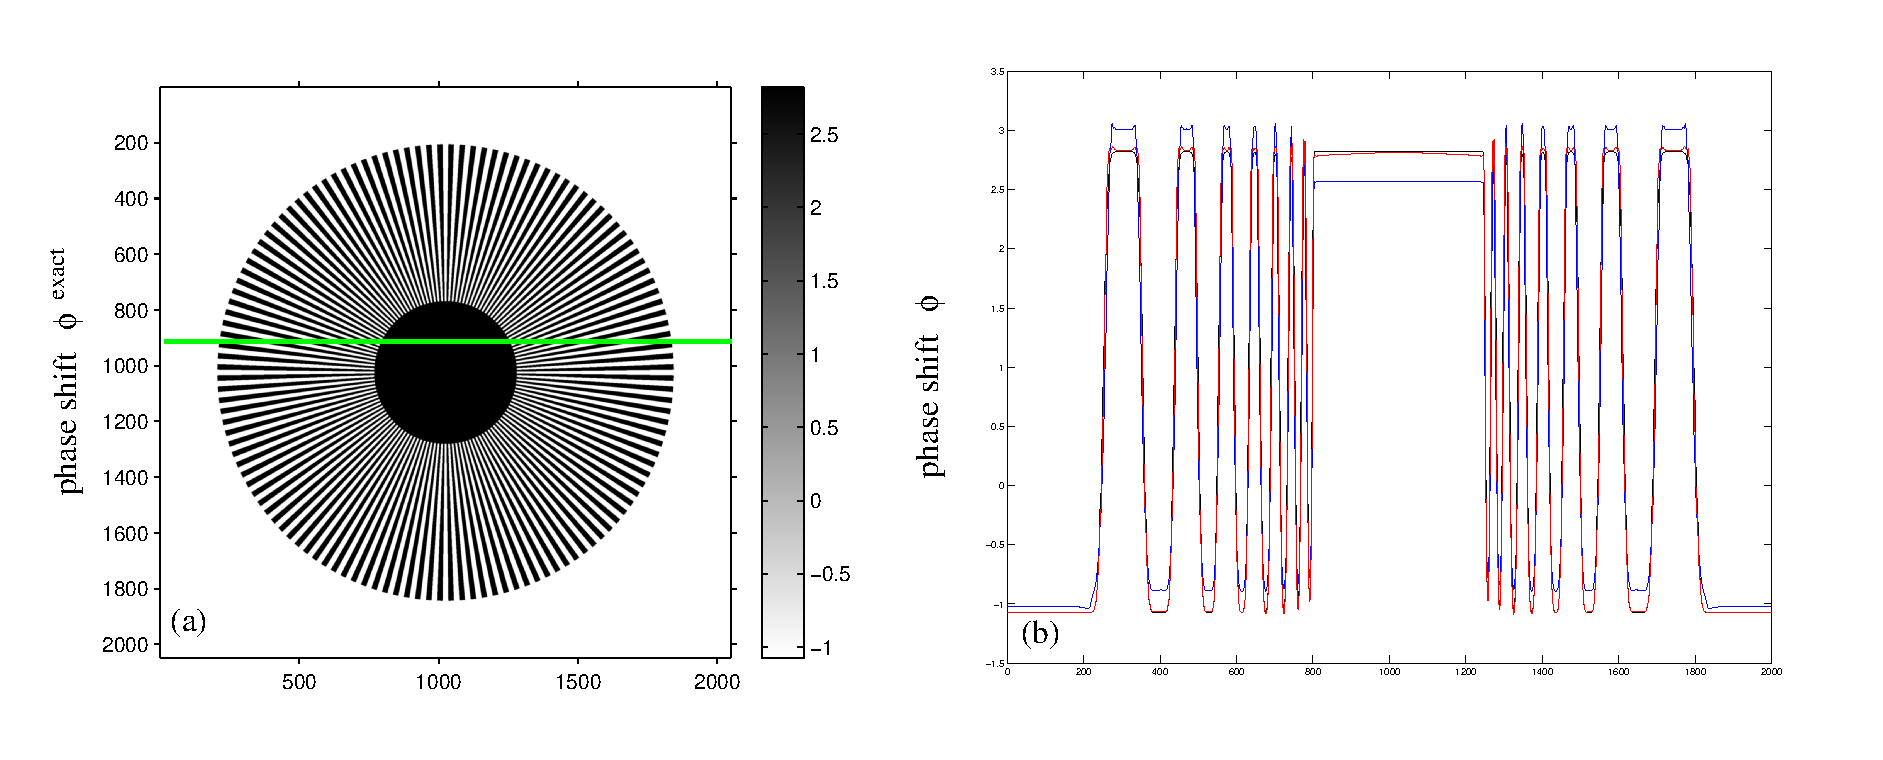
\includegraphics[width=0.99\textwidth]
      {figures/PerturbationTheory/PT-3-SiemensStarThick}};
    \draw[](-0.47*\xx,0.5)node[rotate=90,right,fill=white!100]
    {\qquad\quad $\phi\hon{exact}$ \qquad\qquad };
    \draw[](-0*\xx,1)node[rotate=90,right,fill=white!100]
    {\qquad\quad $\phi$ \qquad\qquad };
  \end{tikzpicture}
  % \psfragfig[width=0.99\textwidth]
  % {figures/PerturbationTheory/PT-3-SiemensStarThick}
  \caption[Leading-order phase retrieval and next-to-leading-order
  correction from propagated intensity of a modified Siemens-star
  phase object.]{% Modified
    Phase maps of a Siemens star with 256 spokes in central projection
    at a resolution of 2048 $\times$ 2048 pixels.  (a) Exact phase map
    at $z=0$.  (b) Line cut through exact phase map (black),
    leading-order result for phase retrieval (blue), and for phase
    retrieval including next-to-leading order (red) at
    $z=\SI{0.3}{m}$.  For the error measure we have
    $\avgn{\Psi\ho{LO}}=\num{0.1535}$ and
    $\avgn{\Psi\ho{LO+NLO}}=\num{0.0347}$, respectively.  Image
    adopted with slight modifications from \cite{Moosmann2010opex}}
    \label{fig:siemens-star-thick}
\end{figure}
%%%%%%%%%%%%%%%%%%%%%%%%%%%%%%%%%%%%%%%%%%%%%%%%%%%%%%%%%%%%%%%%%%%%%%
Phase retrieval to leading and next-to-leading order is indicated in
\cref{fig:siemens-star}.  Simulations were performed for a central
projection of the Siemens star with $\delta_\omega=\num{e-7}$ at an
X-ray energy of $E=\SI{30}{keV}$ on a $\delta_\omega=0$ background,
and for a thickness $d=\SI{0.256}{mm}$.  In order to avoid problems
arising from unresolvable spokes segments, we introduced a central
disk with constant phase shift at the centre of the Siemens star.  The
exact phase map, from which the intensity is computed by free-space
propagation, is obtained from a Gaussian blurred version of the
Siemens star.  This is to avoid extreme phase jumps at object edges.

As \cref{fig:siemens-star}(e) and (f) indicates, the difference map
$\Psi$ decreases when next-to-leading corrections are taken into
account.  To investigate the dependence on distance and resolution of
the retrieved phase, we have considered line cuts through the phase
map as indicated in \cref{fig:siemens-star}(a) and shown in
\cref{fig:siemens-star-cuts}.  When the standard deviation of the
Gaussian blur is kept constant at 1.5 pixels, results do not change
substantially for values of $\delta_\omega$ smaller than \num{e-7}.
(At a higher resolution the averaged-over length scale is thus
shorter.)  However, for $\delta_\omega>\num{e-6}$ strong deviations of
retrieved from exact phase maps occur, both to leading order and
next-to-leading order.  This suggests that the assumption of weak
phase variations to be violated.  Strong phase variations yield large
values of the coefficients in the power series of
\cref{eq:formal-power-series}, impairing the convergence properties of
the expansion.

Including next-to-leading order corrections closely retrieves the
exact phase at a low pixel resolution (or large physical blurring
scale), see left column in \cref{fig:siemens-star-cuts}.  This holds
for all distances $z$ as indicated in \cref{fig:siemens-star-cuts}.
At high spatial resolution, phase retrieval is still observed to be
improved, but edge-related artifacts induced by a stronger varying
phase (smaller physical blurring scale) occur, see right column in
\cref{fig:siemens-star-cuts}.  Increasing the spatial resolution at a
fixed physical blurring scale we observe quantitatively stable
results.

A more complex situation is investigated in
\cref{fig:siemens-star-thick}, where the numbers of spokes in the
Siemens star is increased and a large central disk is added.  Thereby
a hierarchy of scales is introduced to the object, given by the
typical diameter of a spoke to the diameter of the disk.  Comparing
this case with the first line of \cref{fig:siemens-star-cuts}, the
leading-order result is observed to deviate much stronger from the
exact phase in \cref{fig:siemens-star-thick} than in
\cref{fig:siemens-star-cuts}.  In particular, the leading-order
retrieval in \cref{fig:siemens-star-thick} overestimates phase shifts
introduced by the spokes and underestimates phase shifts for the
central region.  When including corrections to next-to-leading order,
we yield a significantly improved phase retrieval which makes up for a
$\sim\SI{10}{\percent}$ deviation of the leading-order result.  In
\cref{fig:siemens-star-thick} the tendency of leading-order retrieval
to over- or underestimate the phase shift is remedied, such that the
mean value remains at zero at a slightly overestimated background to
leading order and a well retrieved background when including
next-to-leading order corrections.  Phase retrieval beyond leading
order being more accurate is due to the non-linearity of the
corrections (maximal difference in phase shifts $\sim 4$).  The
inclusion of all powers of the Laplacian (\acs{ctf}) but exclusion of
non-linear corrections is expected to have improved on the
edge-related artifacts only.

%%%%%%%%%%%%%%%%%%%%%%%%%%%%%%%%%%%%%%%%%%%%%%%%%%%%%%%%%%%%%%%%%%%%%%
%%%%%%%%%%%%%%%%%%%%%%%%%%%%%%%%%%%%%%%%%%%%%%%%%%%%%%%%%%%%%%%%%%%%%%
%\cleardoublepage
\section{Quasiparticle approach}
\label{sec:qp}


In the previous section we have discussed the relation between exit
phase $\phi_0\equiv\phi_{z=0}$ and propagated intensity contrast
$g_{z}$ in Fresnel theory, evading an exact inversion of the forward
problem.  This is due to couplings of transverse derivatives of
$\phi_0$ contributing non-linearly with up to infinite powers to
$g_{z}$ \cite{Moosmann2010opex}.  An expression up to quadratic order
in $\phi_0$ is given in \cref{eq:fresnel-limit-1}.  Large phase
variations $\delta\phi_0$ thus represents strongly coupled classical
fields, excluding a perturbative approach to the inverse problem as in
\cref{sec:perturbation-theory}.  Upon identifying a scaling symmetry
of the exit phase in the limit of vanishing phase variations
$\phi_0\to 0$ through the global U(1) phase-shift invariance and
analysing of how this symmetry is explicitly and dynamically broken by
finite $\delta\phi_0$, the phase retrieval problem can be addressed in
an efficient and non-perturbative fashion.  Up to phase variations
$\abs{\dpo}$ in the order of unity, or more precisely up to the point
where scaling symmetry is dynamically unbroken, the essentially
non-linear relation between $\dpo$ and $g_z$ can be rendered
quasi-linear.  This is reminiscent of the quasiparticle approach to
systems of moderately interacting point particles - a ubiquitous
concept in condensed-matter and plasma physics and quantum field
theory \cite{Landau1957,Abrikosov1959,HofmannBook}.

Fortuitously, essential characteristics of the linear contrast
transfer persist in the quasiparticle sense. \Ie{} the dependence of
contrast transfer on propagation distance $z$ and shot noise favouring
large values of $z$, the high spatial resolution of the
retrieved phase $\phi_0$, and the feasibility of phase-attenuation
duality for high X-ray energies and/or chemically homogeneous samples.

The analysis presented in the following is closely related to the work
presented in \cite{Moosmann2011opex,Hofmann2011opex,Hofmann2014}.


\subsection{Linear models}
\label{sec:qp-linear-models}

%%%%%%%%%%%%%%%%%%%%%%%%%%%%%%%%%%%%%%%%%%%%%%%%%%%%%%%%%%%%%%%%%%%%%%%
\begin{figure}
  \centering
  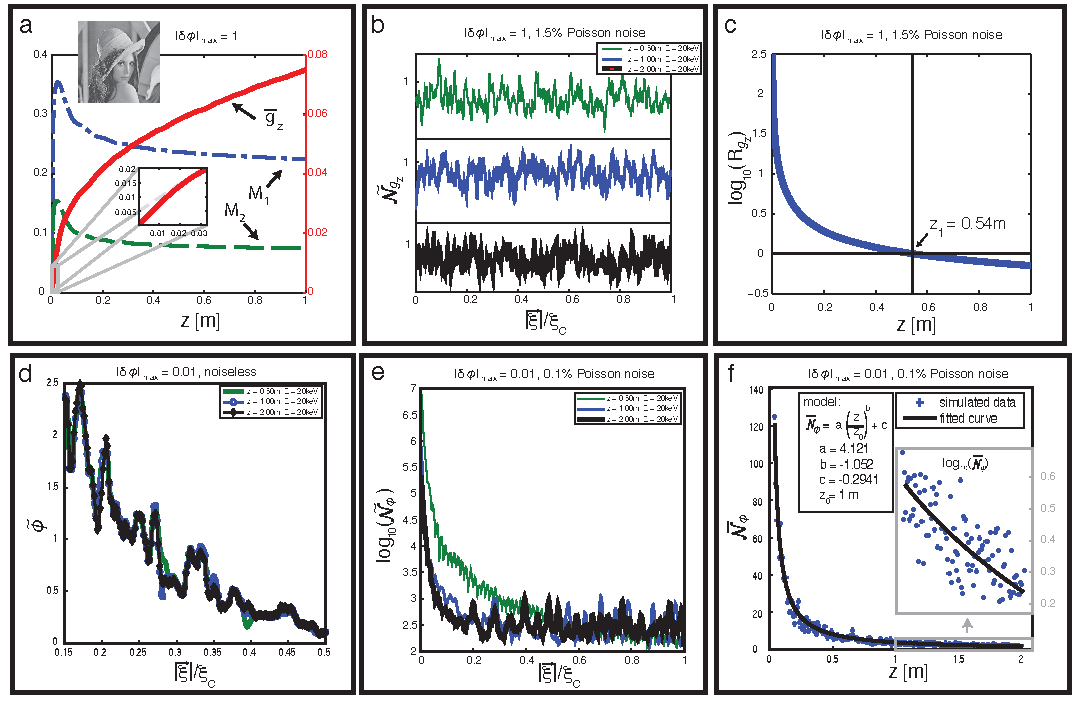
\includegraphics[width=0.99\textwidth]
  {figures/Quasiparticle/Fig2.pdf}
  \caption[Image formation in full Fresnel theory and linear phase
  retrieval for the pure-phase case subject to statistical noise in
  dependence of propagation distance.]{Analysis of image formation in
    full Fresnel theory and linear phase retrieval subject to
    statistical noise and in dependence of propagation distance $z$.
    A pure-phase object is assumed using the Lena test pattern as
    input phase map.  At $E = \SI{20}{keV}$, an exit phase with a
    maximum variation of $\dpom = \num{1}$ is the input for the
    simulated forward propagation used in (a) through (c) and of
    $\dpom = \num{0.01}$ (linear case) in (d) through (f). a,
    Transverse average of modulus of intensity contrast $\mabs{g}_z$,
    and associated first and second moments, $M_1$ and $M_2$, of
    function $\abs{\ft{g}_z}$ in dependence of $z$. The peak positions
    of $M_1$ and $M_2$ indicate maximum edge enhancement.  b, Radial
    spectra $\aft{\N}_{g_z}$, \ie{} the angle averaged modulus of the
    Fourier transform of intensity noise $\N_{g_z}$, for three
    distinct values of $z$ and a shot-noise level of
    \SI{1.5}{\percent} on $I_z$.  Spectra exhibit white-noise nature
    and $z$ independence.  c, Semi-log plot of noise-to-signal ratio
    $R_{g_z}$ (transverse average noise modulus $\mabs{\N}_{g_z}$ to
    transverse average signal modulus of $\mabs{g}_z$).  d, Radial
    spectra $\aft{\N}_{\phi_0}$ of phase retrieved from noiseless
    $g_z$ for three distinct values of $z$.  Spectra are independent
    of $z$.  e, Semi-log plot of radial noise spectra
    $\aft{\N}_{\phi_0}$ of phase maps retrieved from $I_z\hon{noise}$
    subject to \SI{0.1}{\percent} shot noise and for three distinct
    values of $z$.  f, Transverse average of modulus of noise
    $\mabs{\N}_{\phi_0}$ in phase map retrieved from $I_z\hon{noise}$
    subject to \SI{0.1}{\percent} noise as a function of $z$.  Image
    adopted from \cite{Hofmann2014}.}
  \label{fig:qp-2}
\end{figure}
%%%%%%%%%%%%%%%%%%%%%%%%%%%%%%%%%%%%%%%%%%%%%%%%%%%%%%%%%%%%%%%%%%%%%%

Non-deterministic emission of photons by the X-ray source,
light-matter interactions within the object, and the detection process
entail random fluctuations of the noiseless intensity $I_z$.  In the
case of negligible camera dark currents or directly converting
single-photon counting detectors, these fluctuations can effectively
be modelled by Poisson statistics (shot noise).  Invoked by short
exposure times, shot noise then dominates.  Predominantly impairing
intensity contrast at small scales, shot noise in the intensity is a
limiting factor reducing the maximum spatial resolution of $2\,\Delta
x$ in the retrieved phase map.  Given an X-ray beam of sufficiently
high coherence, we now show on simulated phantom data that the average
\acf{snr} of $g_z$ enhances with increasing values of the propagation
distance $z$.  Phantom data is generated upon computing intensity maps
from an exit wave front by forward propagation using full Fresnel
theory (\cref{eq:fresnel}).  A pure-phase object is assumed with the
Lena test pattern (512 $\times$ 512 pixels) used as phantom, see
\cref{fig:phantom-lena,fig:qp-2}(a).  The Lena test pattern is
immersed in a background of zero phase shift with 1024 $\times$ 1024
pixels (symmetric zero padding).

Assuming perfect spatio-temporal coherence, parallel\hyph beam
incidence, and neglecting the effects of shot noise, a two-fold
application of the Fresnel diffraction integral (see \cref{sec:ctf})
yields
\begin{equation}
  \label{eq:guigay-2}
  \begin{split}
    \ft{I}_z(\vecxip) = 
    \int \Intdd{\vecxp}\exp{(-\ii 2\pi\vecxp\vecxip)} 
    \Psi_0\left(\vecxp-\tfrac{\lambda z}{2}\vecxip\right) 
    \Psi^*_0\left(\vecxp+\tfrac{\lambda z}{2}\vecxip\right)\;,
  \end{split}
\end{equation}
where $\ft{I}_z\equiv\F I_z$ demands Fourier transform of $I_z$ as in
\cref{eq:ft-xi-2}.  In the pure-phase case ($B=0$) the exit wave
fields reads $\Psi_0=\Iin\expp{\ii\phi_0}$.  Expanding the exponential
in $\Psi_0$ up to quadratic order in $\phi_0$, yields upon
substitution into \cref{eq:guigay-2} and use of the convolution
theorem (\cref{eq:convolution-theorem-xi})
\begin{equation}
  \label{eq:guigay-expansion}
    \begin{split}
      \ft{g}_z(\vecxip) ={}& 
      2\sin(\pi\lambda z\vecxi^2)\ft{\phi}_0(\vecxi) 
    \\ &  -\cos(\pi\lambda z\vecxi^2)\int\Intdd{\vecxi'}
      \ft{\phi}_0(\vecxi')\,\ft{\phi}_0(\vecxi-\vecxi')
    \\ & +\expp{\ii\pi\lambda z\vecxi^2}\int\Intdd{\vecxi'}
    \expp{-\ii 2\pi\lambda z\vecxi\cdot\vecxi'} 
    \ft{\phi}_0(\vecxi')\,\ft{\phi}_0(\vecxi-\vecxi')
    \\ & +O( ( \ft{\phi}_0 )^3 ) \;.
  \end{split}
\end{equation}
Given that $\phi_0$ satisfies the \ac{ctf} criterion of weakly varying
phases, %\eqref{eq:weak-phase},
\begin{equation}
  \label{eq:weak-phase-2}
  \abs{\delta\phi_0}\equiv\abs{
    \phi_0\left(\vecxp-\tfrac{\lambda z}{2}\vec{\vecxip}\right)
    - \phi_0\left(\vecxp+\tfrac{\lambda z}{2}\vec{\vecxip}\right)}
  \ll 1\;,
\end{equation}
the right-hand side of \cref{eq:guigay-expansion} can be truncated at
linear order in $\ft\phi_0$, restoring linear transfer of contrast
from $\ft{\phi}_0$ to $\ft{g}_z$ as
\begin{equation}
  \label{eq:ctf-g-2}
    \ft{g}_z(\vecxip) =
     2\ft{\phi}_0(\vecxip)\sin(\pi\lambda z\vecxip^2) \;,
\end{equation}
which is the known \acf{ctf}.  Provided that $\ft{g}_z$ exhibits zeros
of the same order as those of the sine function in \cref{eq:ctf-g-2},
which are given by
\begin{equation}
  \label{eq:sine-zeros}
  \abs{\vecxip}_m\equiv\sqrt{\frac{m}{\lambda z}} \;, 
  \quad m=\{0,1,2,\cdots\} \;,
\end{equation}
\ac{ctf} retrieval in Fourier space does not produce singularities.

In the limit $z\to0$, the power-series expansion in
\cref{eq:guigay-expansion} is dominated by the linear-in-$z$ part of
the linear-in-$\ft{\phi}_0$ term, and  linearised \ac{tie}
\eqref{eq:tie-linear-fourier} is recovered.  In the following we will
refer to the algebraic inversion of \cref{eq:tie-linear-fourier} as
Paganin phase retrieval \cite{PaganinBook}.  Comparing the inverse
transfer functions related to Paganin and \ac{ctf} retrieval as
depicted in \cref{fig:phase-filter}, Paganin phase retrieval is
observed to suppresses high-frequency information within the frequency
band of
\begin{equation}
  \label{eq:paganin-frequency}
  \xi_P\equiv \frac{1}{\sqrt{2\lambda z}} < \abs{\vecxip} < \xi_c \;.
\end{equation}
The spatial cut-off frequency $\xi_c$ is set by the effective linear
pixel size $\Delta x$ to $\xi_c=\frac{1}{2\Delta x}$.  Unless
$\xi_c\propto\xi_P$ (\cref{fig:qp-2}(a)), Paganin phase retrieval
depletes attainable compared to the maximum resolution set by the
pixel size to $2\Delta x$.  For $E=\SI{20}{keV}$ and $\Delta
x=\SI{1}{\micro m}$, this already occurs at $z\approx\SI{3.2}{cm}$.
The short exposure times typically required for in vivo imaging result
in count rates per pixel in the order of 4500.  Imaging at such low
values of $z$, intensity contrast $g_z$ is unacceptably low compared
to the high shot noise.  The associated noise-to-signal ratio is
denoted by $R_{g_z}$ (see \cref{fig:qp-2}(c)).  Conveniently, we
define the maximum absolute phase variation $\dpom$ as the maximum of
the left-hand-side of \cref{eq:weak-phase-2} over all admissible
values of $\vecxp$ and $\vecxip$: $\dpom = \max{\abs{\dpo}}$.
Furthermore, we introduce the average signal modulus $\mabs{g}_z$ and
the associated spectral moments $M_1$ and $M_2$.  $\mabs{g}_z$ is
defined as the average of the modulus of the intensity contrast
\begin{equation}
  \label{eq:mean-abs-g}
  \mabs{g}_z \equiv \avgabs{g_z} \equiv 
  \frac{1}{A_\fov} \int_{\fov}\Intdd{\vecxp}\abs{g_z(\vecxp)}\;,
\end{equation}
where the normalisation factor $A_\fov$ is the area related to the
\acf{fov} of detector
\begin{equation}
  \label{eq:afov}
  A_\fov \equiv \int_{\fov}\Intdd{\vecxp} \;.
\end{equation}
The $i$-th spectral moment is defined as
\begin{equation}
  \label{eq:spectral-moments}
  M_i \equiv \frac{1}{\int\Intdd{\vecxip}} \int\Intdd{\vecxip}
   \frac{\abs{\vecxip}}{\xi_c}^i \abs{\ft{g}_z(\vecxip)} \;,
\end{equation}
where the region of integration is set by the cut-off frequency
$\xi_c$.  Thus the normalisation factor \cref{eq:spectral-moments}
reads $\frac{1}{\int\Intdd{\vecxip}}=(\Delta x)^2$.  The behaviour of
$\mabs{g}_z$, and the spectral moments $M_1$ and $M_2$ as function of
propagation distance $z$ is depicted in \cref{fig:qp-2}(a) for phase
variations of $\dpom=1$.  As implied by linearised \ac{tie}, there is
a linear rise of $\mabs{g}_z$ due to local contrast growth at edges of
$\phi_0$ up to the peak position $z_P$ of $M_1$ and $M_2$ where
maximum edge enhancement occurs.  Though the amplitude of a given
fringe saturates as $z$ increases, the average signal modulus
$\mabs{g}_z$ still increases beyond $z_P$.  This is due to the tiling
of the field of view through multiple, resolvable fringes per edge.

\subsection{Influence of noise}
\label{sec:qp-noise}

In the following we investigate how this situation is influenced by
shot noise.  We define the noise of $\N_Q$ of a quantity $Q$ as the
difference between $Q$, evaluated for a given noise level of $I_z$,
and $Q$, evaluated on the noiseless intensity $I_z$,
\begin{equation}
  \label{eq:noise}
  \N_Q(I_z) \equiv Q(I_z\hon{noise}) - Q(I_z) \;.
\end{equation}
Analogue to \cref{eq:mean-abs-g}, we define the average noise modulus
of $g_z$ as
\begin{equation}
  \label{eq:mean-abs-noise}
  \mabs{\N}_{g_z} \equiv 
  \frac{1}{A_\fov} \int_{\fov}\Intdd{\vecxp}\abs{\N_{g_z}(\vecxp)} \;,
\end{equation}
with $A_\fov$ as in \cref{eq:afov}.  The noise-to-signal ratio then
reads
\begin{equation}
  \label{eq:nsr}
  R_{g_z} = \frac{\mabs{\N}_{g_z}}{\mabs{g}_z} \;.
\end{equation}
\Cref{fig:qp-2}(c) depicts $R_{g_z}$ assuming a shot-noise level of
\SI{1.5}{\percent} on $I_z$.  While $R_{g_z}$ is large for $z<z_1$, it
falls below unity beyond $z=z_1$, and continuously approaches zero for
$z\to\infty$ as implied by the behaviour of $\mabs{g}_z$ and
$\N_{g_z}$ in \cref{fig:qp-2}(a,b).  Experimentally, the
propagation distance cannot be raised indefinitely due to partial
spatial coherence.  According to the van-Cittert-Zernike theorem
(\cref{eq:van-cittert-zernike-far-field}), the spatial extent of an
incoherently emitting source introduces a blurring of sample points in
the detected intensity maps.  Using
\cref{eq:cut-off-frequency-blurring}, the blur $b$ relates to the
propagation-induced transverse coherence length $l_\perp$
(\cref{eq:coherence-length}) as
\begin{equation}
  \label{eq:blur}
  b \approx \frac{1}{2\xi_b} \approx \frac{\lambda z}{2 l_\perp} \;,
\end{equation}
where $\xi_b$ denotes the blurring-induced cut-off frequency.  Only if
$b\lesssim \Delta x$ does contrast transfer (in Fourier space) reach
the cut-off frequency $\xi_c$ in compliance with
\cref{eq:weak-phase-2}.  Otherwise, the source function suppresses
frequencies in $\ft{g}_z$ above $\xi_b\sim\frac{l_\perp}{\lambda z}$
\cite{BornWolf,Wolf}.

Let us now consider the influence of shot noise on the retrieved
phase.  Therefore, we define the radial phase spectra and the
associated radial noise spectra as
\begin{equation}
  \label{eq:phi-radial-spectra}
  \aft{\phi}_0(\xip) \equiv 
  \frac{1}{2\pi A_\fov}\int_0^{2\pi}\Intd{\theta}\absn{\ft{\phi}_0}
\end{equation}
and
\begin{equation}
  \label{eq:phi-noise-radial-spectra}
  \aft{\N}_{\phi_0}(\xip) \equiv 
  \frac{1}{2\pi A_\fov}\int_0^{2\pi}\Intd{\theta}
  \absn{\ft{\N}_{\phi_0}} \;,
\end{equation}
with $A_\fov$ as in \cref{eq:afov}.  \Cref{fig:qp-2}(d,e) depicts the
radial spectra $\aft{\phi}_0$ and the associated radial noise spectra
$\aft{\N}_{\phi_0}$ of the phase retrieved from \ac{ctf} for three
distinct values of $z$.  While the radial spectra $\aft{\phi}_0$ are
approximately independent of $z$ (\cref{fig:qp-2}(d)), the radial
noise spectrum $\aft{\N}_{\phi_0}$ as well as the average noise
modulus $\mabs{\N}_{\phi_0}$ fall off with increasing $z$ as shown in
\cref{fig:qp-2}(e) and (f), respectively.  

We continue by analysing the $z$-dependence of the average noise
modulus of the retrieved phase.  We have
\begin{equation}
  \label{eq:mean-phase-noise-modulus-0}
  \begin{split}
      \mabs{\N}_{\phi_0} & = \avgabs{\phi_0\hon{noise}-\phi_0}
      \\ &= \avgabs{ \iF\frac{\F g_z\hon{noise}}{f(\abs{\vecxip})} 
      -\iF\frac{\F g_z}{f(\abs{\vecxip})} }
  \\ & =\avgabs{ \iF\frac{\F \N_{g_z}}{f(\abs{\vecxip})} } \;,
  \end{split}
\end{equation}
with $\phi_0$ and $g_z$ evaluated on the noiseless intensity $I_z$,
and $f(\abs{\vecxip})$ denoting one of the transfer functions in
\cref{eq:tie-linear-fourier,eq:ctf-g,eq:ctf-dual,eq:tie-dual},
respectively.  The value of $\mabs{\N}_{\phi_0}$ is dominated by the
low-frequency components on the right-hand side of
\cref{eq:mean-phase-noise-modulus-0}, which we thus may approximate as
\begin{equation}
  \label{eq:mean-phase-noise-modulus-1}
  \begin{split}
    \mabs{\N}_{\phi_0} = 
    \avgabs{ \iF\frac{\F \N_{g_z}}{f(\abs{\vecxip})} }
    & \propto \avgabs{ \iF\frac{\F \N_{g_z}}
      { f(\abs{\vecxip}\approx 0) } }
    \\ & \propto \frac{\avgabs{ \iF \F\N_{g_z} }}
    {f(\abs{\vecxip}\approx 0)} 
    \\ & \propto \frac{\avgabs{ \N_{g_z} }}
    {f(\abs{\vecxip}\approx 0)} \;.
  \end{split}
\end{equation}
Close to $\abs{\vecxip}=0$, the transfer function of
\cref{eq:tie-linear-fourier,eq:ctf-g,eq:ctf-dual,eq:tie-dual} are
approximated by
\begin{equation}
  \label{eq:transfer-function-0}
  \begin{split}
    f(\abs{\vecxip}\approx 0) 
    & \approx 2\left.\lrp{\pi\lambda z\vecxip^2 
    +\epsilon}\right|_{\abs{\vecxip}\approx 0}
  \\ & \approx 2\lrp{\frac{\pi\lambda}{L^2}z +\epsilon} \;,
  \end{split}
\end{equation}
where have substituted the smallest finite value for
$\abs{\vecxip}=\frac{1}{L}$, $L$ being the linear extend of a square
detector.  Here, $\epsilon$ is a small constant denoting either the
duality parameter of \cref{eq:ctf-dual} or an ad hoc regularisation as
in \cref{eq:regularisation-sine,eq:zero-regularisation}.  For
moderately varying phases, $\dpom\lesssim 1$, variations of the
intensity contrast are of the order $\mathcal{O}(1)$.  Beyond edge
enhancement, the (average) signal rises approximately with
$g_z\propto\sqrt{z}$, see \cref{fig:qp-2}(a) and
\cref{fig:fringe-evolution}.  Thus, since shot noise obeys Poisson
statistics, $\N_{g_z}$ increases as $\sqrt[4]{z}$ and can be
considered constant.  As a consequence, we infer from
\cref{eq:mean-phase-noise-modulus-1,eq:transfer-function-0} that phase
noise decreases like $z^{-1}$ as image detection moves towards the
far-field regime:
\begin{equation}
  \label{eq:phase-noise}
      \mabs{\N}_{\phi_0} \propto \frac{1}{z} \;,
\end{equation}
which is confirmed by the fit of \cref{fig:qp-2}(f).


\subsection{Quasiparticle transfer of contrast}
\label{sec:qp-ctf}

%%%%%%%%%%%%%%%%%%%%%%%%%%%%%%%%%%%%%%%%%%%%%%%%%%%%%%%%%%%%%%%%%%%%%%
\begin{figure} 
  % Plots created from Matlab function phdFig_PhaseFilter_QP
  \centering
  \psfragfig[
  width=0.75\textwidth,
  height=0.24\textheight
  ]
  {figures/PhaseFilter_QP/Fig1}{
    \small
    \psfrag{xlabel}[c][c]{$\;\abs{\vecxip}/\xic$}
    \psfrag{ylabel}[c][l]{Inverse transfer function}
    \psfrag{0.2}{0.2} \psfrag{0.4}{0.4} \psfrag{0.6}{0.6} 
    \psfrag{0.8}{0.8} \psfrag{1}{1} \psfrag{0}{0}
    \psfrag{-5}{-5} \psfrag{0}{0} \psfrag{5}{5} 
    \psfrag{data1}{$\tie$}
    \psfrag{data2}{$\ctf$}
    \psfrag{data3}{$\qp$}
    \psfrag{data4}{$\qpc$}  }
  \caption[Fourier space filter (regularised inverse transfer
  functions) for linear and quasilinear phase retrieval.]{Radial
    dependence of inverse transfer functions related to linearised
    $\tie$, $\ctf$, quasiparticle ($\qp$), and modified quasiparticle
    ($\qpc$) approaches, see
    \cref{eq:linear-tie-phase,eq:ctf-phase,eq:qp,eq:qpc},
    respectively.  Regularisation as in \cref{eq:zero-regularisation}
    was used for $\tie$, and as in \cref{eq:regularisation-sine} for
    $\ctf$, $\qp$, and $\qpc$.  Energy was set to $E=\SI{12.4}{keV}$
    ($\lambda=\SI{e-10}{m}$), propagation distance to $z=\SI{0.1}{m}$,
    and pixel size to $\Delta x = \SI{1}{\micro m}$, the
    regularisation parameter to $\alpha=\num{e-1}$, and the threshold
    for quasiparticle retrieval to $\delta=\num{0.2}$.  In the
    interest of clearer presentation, we have chosen values of
    $\alpha$ and $\delta$ considerably larger than the usually
    employed values for real data ranging between \num{e-2} and
    \num{e-3}, and \numrange{e-2}{e-1}, respectively.  The maximal
    cut-off frequency is $\xic=(2\Delta x)^{-1}$.  The argument of
    depicted transfer function is $x=\frac{\pi\lambda z}{(2\Delta
      x)^2}\frac{\abs{\vecxip}^2}{\xic^2} =
    2.5\pi\frac{\abs{\vecxip}^2}{\xic^2}$.}
  \label{fig:phase-filter-qp}
\end{figure}
%%%%%%%%%%%%%%%%%%%%%%%%%%%%%%%%%%%%%%%%%%%%%%%%%%%%%%%%%%%%%%%%%%%%%%

The weakly varying phase condition $\dpom\ll1$ does usually not comply
with requirements imposed by in vivo \acf{xpct} for developmental
biology, see \cref{cha:bio}.  \Eg{} an early-stage frog embryo of
\SI{1}{mm} diameter would produce an absolute phase shift of 152 at an
X-ray energy of $\SI{30}{keV}$, assuming a mean value of the real
refractive index decrement of $\delta_\omega=\num{e-6}$.  Thus
assuming a phase variation of $\SI{1}{\percent}$, we have
$\dpom\approx\num{1.5}$, violating the validity of \ac{ctf} phase
retrieval.  This would call for an exact inversion of
\cref{eq:guigay-expansion}, impossible to attain analytically.

In order to construct an approximation to the solution of
\cref{eq:guigay-expansion} based on a single-distance intensity
measurement, we appeal to symmetry considerations as a guiding
principle.  \Cref{eq:guigay-2} and every order in $\phi_0$ in
\cref{eq:guigay-expansion} are observed to be invariant under global
phase shifts 
\begin{equation}
  \label{eq:global-phase-shift-u1}
  \Psi_0\to\expp{\ii\alpha}\Psi_0
  = \sqrt{I_0} \expb{\ii\lrp{1+\frac{\alpha}{\phi_0}}} \;,
\end{equation}
where $\alpha$ is a real parameter which determines how this global
U(1) symmetry acts on $\Psi_0$.  In the limit $\dpom\to0$ with
$\phi_0$ remaining finite the factor ${1+\frac{\alpha}{\phi_0}}$
becomes a real constant $S$.  Thus an invariance under global phase
shifts  transmutes into a symmetry under global phase scaling
\begin{equation}
  \label{eq:upscaling}
   \phi\to S\phi \;.
\end{equation}

%%%%%%%%%%%%%%%%%%%%%%%%%%%%%%%%%%%%%%%%%%%%%%%%%%%%%%%%%%%%%%%%%%%%%%
\begin{figure}
  \centering
  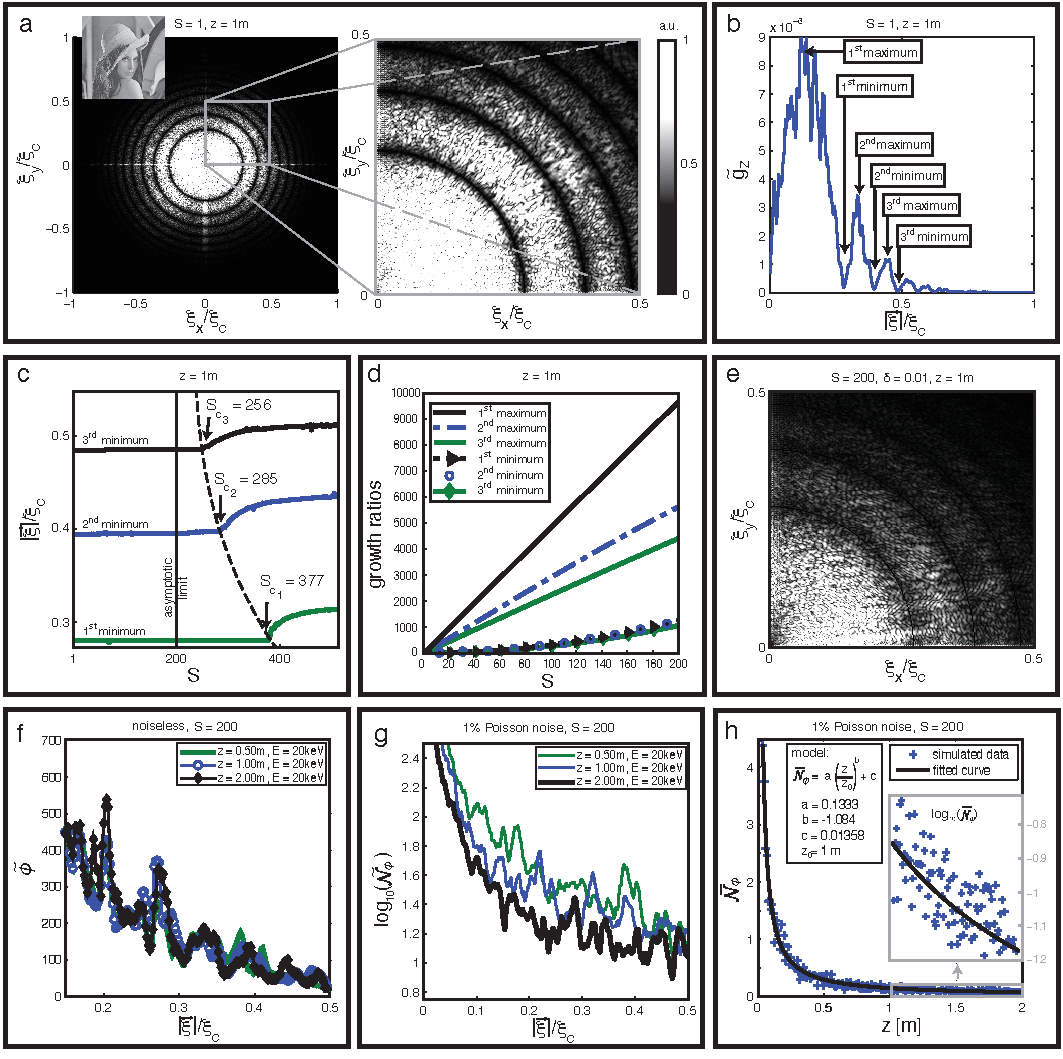
\includegraphics[width=0.99\textwidth]
  {figures/Quasiparticle/Fig3.pdf}
  \caption[Quasiparticle behaviour of relation between intensity
  contrast and phase up to criticality under simulated Fresnel forward
  propagation.]{Quasiparticle behaviour of contrast transfer from
    phase to intensity up to criticality under simulated Fresnel
    forward propagation at $E = \SI{20}{keV}$.  A maximum exit phase
    variation of $\dpom = \num{0.01}$, referring to the linear case
    with $S = \num{1}$, is used as input for (a) and (b).  In the
    non-linear case of (e) through (h) $S = \num{200}$, corresponding
    to $\dpom = \num{2}$, is used.  In (a) through (e), the
    propagation distance is fixed at $z = \SI{1}{m}$.  a, Modulus of
    Fourier transform $\abs{\ft{g}_z}$ of intensity contrast $g_z$.
    b, Radial spectrum $\aft{g}_z$.  First three minima at positions
    $\abs{\vecxip}_1$, $\abs{\vecxip}_2$, and $\abs{\vecxip}_3$ are
    clearly discernible.  c, Minima positions $\abs{\vecxip}_1$,
    $\abs{\vecxip}_2$, and $\abs{\vecxip}_3$ in dependence of $S$,
    upscaling the linear case.  $S_{c_m}$ appears to converge to a
    finite value of about $\num{200}$ in the hypothetical
    (infinite-resolution) limit $m\to\infty$.  d, Growth ratios: First
    three maxima and minima normalised to first minimum at $S=\num{1}$
    in dependence of $S$.  e, Modulus of Fourier transformed modified
    intensity contrast, as defined in \cref{eq:qpc}, for
    $\delta=\num{0.01}$. f, Radial spectra $\aft{\phi}_0$ of the phase
    retrieved from noiseless $g_z$, exhibiting independence of $z$.
    g, Semi-log plot of the radial noise spectra $\aft{\N}_{\phi_0}$
    of phase retrieved from $I_z$ subject to \SI{1}{\percent} shot
    noise for three distinct values of $z$.  h, Transverse average of
    modulus of noise $\mabs{\N}_{\phi_0}$ in the phase retrieved from
    $I_z$ subject to \SI{1}{\percent} Poisson noise as function of
    $z$.  Image adopted from \cite{Hofmann2014}.}
  \label{fig:qp-3}
\end{figure}
%%%%%%%%%%%%%%%%%%%%%%%%%%%%%%%%%%%%%%%%%%%%%%%%%%%%%%%%%%%%%%%%%%%%%%
To elucidate the dynamics of forward propagation in Fresnel theory, we
examine in what sense scaling symmetry persists at finite values of
$\dpom$.  Therefore we investigate the behaviour of the radial
intensity spectrum  $g_z$ under upscaling of the exit phase map as in
\cref{eq:upscaling}, see \cref{fig:qp-3}(a,b)
\cite{Moosmann2011opex,Hofmann2011opex}.  The radial intensity
contrast spectrum is defined analogue to \cref{eq:phi-radial-spectra}
as
\begin{equation}
  \label{eq:g-radial-spectrum}
  \aft{g}_z\equiv 
  \frac{1}{2\pi A_\fov}\int_0^{2\pi}\Intd{\theta}\abs{\ft{g}_z} \;.
\end{equation}
By forward propagation simulated in full Fresnel theory, the zeros of
$\aft{g}_z$ at $\abs{\vecxip}_m\equiv\sqrt{\frac{m}{\lambda z}}$, as
predicted by the linear-in-$\phi_0$ \ac{ctf} relation, turn into
minima at finite values of $\dpom$.  Under upscaling the phase
$\phi_0$ from the linear regime, where $\dpom\ll 1$ at $S=1$, the
positions of these minima remain fixed at $\abs{\vecxip}_m$ up to a
critical value $S_c\gg 1$, where to phase variations
$\abs{\delta\phi_0}$ substantially above unity (\cref{fig:qp-3}(c)).
The constancy of $\abs{\vecxip}_m$ under phase upscaling necessitates
the contribution of all orders on the right-hand-side of
\cref{eq:guigay-expansion} \cite{Hofmann2011opex}.  A truncation of
\cref{eq:guigay-expansion} to finite, but beyond linear order in
$\phi_0$ would not exhibit such a behaviour.

Beyond critical upscaling $S>S_c$, the minima positions of
$\aft{g}_z$ start to move like order parameters as in second-order
phase transitions, see \cref{fig:qp-3}(c) for $m=\{1,2,3\}$.
Moreover, the simulated data suggests the existence of a finite
asymptote for $m\to\infty$ at $S_{c_m}$, $\forall m\ge1$.

We continue by investigating of how the information of $g_z$ is the
distributed in Fourier space.  Let $\abs{\vecxip}_{m,m-1}$ denote the
positions of the maxima of $\ft{g}_z$ in between adjacent minima at
$\abs{\vecxip}_{m}$ and $\abs{\vecxip}_{m-1}$.  Furthermore, we define
growth ratios of the maxima and minima as
\begin{equation}
  \label{eq:maxima-growth}
  R_{m,m-1}(S) \equiv 
  \frac{\aft{g}_z(\abs{\vecxip}_{m,m-1})(S)}
  {\aft{g}_z(\abs{\vecxip}_{1})(S=1)}
\end{equation}
and
\begin{equation}
  \label{eq:minima-growth}
  R_{m}(S) \equiv 
  \frac{\aft{g}_z(\abs{\vecxip}_{m})(S)}
  {\aft{g}_z(\abs{\vecxip}_{1})(S=1)} \;,
\end{equation}
respectively.  The dependencies of $R_{m,m-1}$ and $R_{m}$ on $S$ are
depicted in \cref{fig:qp-3}(d) for $m=\{1,2,3\}$.  Here, we observe a
linear behaviour in $S$ for $R_{m,m-1}$ and a non-linear one for
$R_{m}$.  Moreover, the curves $R_{m}$ of minima growth ratios are
degenerate.  This indicates that non-linear terms in
\cref{eq:guigay-expansion} conspire to add up to a correction periodic
in $\pi\lambda z\vecxip^2$ and independent of $S$.  Thus, the bulk of
information in $\ft{g}_z$ remains localised near the maximum positions
$\abs{\vecxip}_{m,m-1}$ as in the linear \ac{ctf} case when $\dpom\ll
1$ (\cref{fig:qp-3}(b)).

In the following, we will exploit these two properties, the inertness
of the minima positions and the concentration of information near the
maxima, by modifying the intensity contrast in Fourier space such that
a quasi-linear contrast transfer is maintained as in
\cref{eq:ctf-g-2}.  The modified intensity contrast $\qpft{g}_z$
neglects marginal, non-linear intensity contrast near minima positions
$\abs{\vecxip}_{m}$, assuring phase retrieval free of singularities.
The modified intensity contrast is obtained from $g_z$ by means of a
binary filtering of $\ft{g}_z$ for $\pi\lambda
z\vecxip^2>\frac{\pi}{2}$.  Employing the binary filter to the
singularity at zero frequencies would strongly modify the intensity
contrast and distort phase retrieval.  Thus, for vanishing frequencies
a regularisation prescription as described in
\cref{sec:regularisation} is used.  One may define the modified
intensity $\qpft{g}_z$ as
\begin{equation}
  \label{eq:qp}
  \ft{g}_z(\vecxip) \to  \qpft{g}_z(\vecxip) \equiv
  \Theta\lrp{\abs{\sin(\pi\lambda z\vecxip^2)} - \delta} 
  \ft{g}_z(\vecxip) \;,
\end{equation}
where $\Theta$ denotes the Heaviside step function, and $\delta\ll1$
is a real positive constant.  The domain of $\ft{g}_z$ to be modified
follows from \cref{eq:qp} as
\begin{equation}
  \label{eq:rings-derivation}
  \begin{split}
    \delta\ge \absn{ \sin(\pi\lambda z\vecxip^2) } 
    & = \absn{\sin(\pi\lambda z
     (\vecxip^2-\abs{\vecxip}^2_m +\abs{\vecxip}^2_m))}
 \\ & = \absn{\sin(\pi\lambda z(\vecxip^2-\abs{\vecxip}^2_m))}
 \\ & \approx \absn{\pi\lambda z(\vecxip^2-\abs{\vecxip}^2_m)}
 \\ & = \pi\lambda z\abs{(\abs{\vecxip}+\abs{\vecxip}_m)
  (\abs{\vecxip}-\abs{\vecxip}_m)} 
 \\ &\approx \pi\lambda z 2 \abs{\vecxip}_m 
    \abs{\abs{\vecxip}-\abs{\vecxip}_m} \;.
  \end{split}
\end{equation}
For $m\ge1$, we define the set of frequencies within rings by
\begin{equation}
  \label{eq:rings}
  \abs{\vecxip}_\circledcirc \equiv \lrbr{\
   \abs{ \abs{\vecxip} - \abs{\vecxip}_m } \le 
  \frac{\delta}{2\pi\lambda z \abs{\vecxip}_m} }\;.
\end{equation}
Demanding continuity, we may also employ the following modification of
$\ft{g}_z$
\begin{equation}
  \label{eq:qpc}
  %\ft{g}_z(\vecxip) \to  
  \qpft{g}_z(\vecxip) \equiv
  \begin{cases} 
    \frac{1}{\delta}\abs{\sin(\pi\lambda z\vecxip^2)} 
    \ft{g}_z(\vecxip)
    & \mathrm{on\,rings}\abs{\vecxip}_\circledcirc
    \\ \ft{g}_z(\vecxip) & \mathrm{otherwise } \;.
  \end{cases}
\end{equation}
While phase retrieval using \cref{eq:qp} neglects the information
contained within $\abs{\vecxip}_\circledcirc$ completely,
\cref{eq:qpc} takes into account a downsized version of the
information within rings $\abs{\vecxip}_\circledcirc$, see
\cref{fig:phase-filter}.  Practically, we do not observe a difference
in using \cref{eq:qp} or \cref{eq:qpc} for phase retrieval within a
parameter range of $\num{e-3}\le\delta\le\num{e-3}$.  Thus, the
neglect of information within rings $\abs{\vecxip}_\circledcirc$ is
marginal.  This is further justified by considering the support of the
 information filtered in $\ft{g}_z$.  The cut-off frequency, set by the
effective pixel size to $\xic=\frac{1}{2\Delta x}$, defines a disk of
permissible frequencies with an area $A_c=\pi\xic^2$.  Let
$A_{\circledcirc}$ denote the summed area and $\Nrings$ the number of
rings within $\abs{\vecxi}\le\xic$.  The latter is given by
\begin{equation}
  \label{eq:number-of-rings}
  \Nrings = \frac{\pi\lambda z \xic^2}{\pi} 
  = \lambda z \xic^2 \;,
\end{equation}
and the area $A_{\circledcirc}$ calculates as
\begin{equation}
  \label{eq:rings-area-0}
  \begin{split}
      A_{\circledcirc} & = \int_{\abs{\vecxip}_\circledcirc}\Intdd{\vecxip}
        = 2\pi % \sum_m^{\Nrings}
      \int_{\abs{\vecxip}_\circledcirc}\Intd{\abs{\vecxip}}
      \\ & = \pi \sum_m^{\Nrings} \left.\abs{\vecxip}^2\right|
      _{\abs{\vecxip}_m-\frac{\delta}{2\pi\lambda z\abs{\vecxip}_m}}
      ^{\abs{\vecxip}_m+\frac{\delta}{2\pi\lambda z\abs{\vecxip}_m}} 
      \\ & = \frac{2\delta}{\lambda z} \sum_m^{\Nrings} 1
      = \frac{2\delta}{\lambda z} \Nrings
      \\ &  = 2\delta \xic^2 \;.
  \end{split}
\end{equation}
Thus, the ratio of summed annular areas within disk
$\abs{\vecxip}\le\xic$ to the area of the disk reads
\begin{equation}
  \label{eq:filtered-area-ratio}
  R_{\circledcirc} = \frac{A_{\circledcirc}}{A_c} 
  = \frac{2\delta}{\pi} \;,
\end{equation}
which is small since $\delta$ is small.  Thus, the support neglected
in $\qpft{g}_z$ is not only marginal, but independent of experimental
parameters $E$, $z$, and $\Delta x$.  

The presented approach restores linearity between phase and intensity
despite non-linear propagation effects.  This is reminiscent of
quasiparticle dispersion laws.  In this sense, \ac{ctf} represents a
dispersion law between phase and intensity, when phase is associated
with (complex) momentum and intensity with (complex) energy.  Momentum
and energy are parametrised by $\vecxip$ labelling both effective
'particle' species away from $\abs{\vecxip}_m$ and degenerate 'ground
states' at $\abs{\vecxip}_m$.  For $S>0$ scaling symmetry is
explicitly broken by non-linear terms in \cref{eq:guigay-expansion}
rendering the energies of the 'ground states', \ie{} the values of the
minima of $\ft{g}_z$ at $\abs{\vecxip}_m$, finite.  However, for $S\le
S_c$, 'ground states' $\abs{\vecxip}_m$ are invariant under phase
upscaling and thus scaling symmetry remains dynamically unbroken.

\Cref{fig:qp-3}(f) depicts the angular averaged radial spectra of
phase retrieved in the quasiparticle sense from noiseless $g_z$ with
parameters $S=\num{200}$, $\delta=\num{e-2}$, and three distinct
values of $z$.  As in the linear case of \cref{fig:qp-2}(d), the
spectra $\aft{\phi}_0$ are independent of $z$.  This indicates that,
despite large phase variations of $\dpom\approx\num{2}$ and away from
$\abs{\vecxip}_m$, the dependence of non-linear terms on $z$
effectively cancel in \cref{eq:guigay-expansion}.  At a shot-noise
level of \SI{1}{\percent}, the radial noise spectra
$\aft{\N}_{\phi_0}$ (\cref{fig:qp-3}(g)) behave as in the linear case
(\cref{fig:qp-2}(e)).  This is also observed for the average noise
modulus $\mabs{\N}_{\phi_0}$ of the retrieved phase as depicted in
\cref{fig:qp-3}(h), observing the same $z^{-1}$ decay as in
\cref{fig:qp-2}(f).

\subsection[\texorpdfstring{Quasiparticle transfer under global\\
  phase-attenuation duality}{Quasiparticle transfer under global
  phase-attenuation duality}]{Quasiparticle transfer under global
  phase-attenuation duality}
\label{sec:qp-duality}

%%%%%%%%%%%%%%%%%%%%%%%%%%%%%%%%%%%%%%%%%%%%%%%%%%%%%%%%%%%%%%%%%%%%%%
\begin{figure}
  \centering
  \includegraphics[width=0.99\textwidth]
  {figures/Quasiparticle/Fig4.pdf}
  \caption[Global phase-attenuation duality versus upscaling and
  confrontation with experimental data on fixed frog embryo.]{Global
    phase-attenuation duality versus upscaling and confrontation with
    experimental data on fixed frog embryo.  (b) through (f) are based
    on tomographic data of a fixed, four-cell stage Xenopus frog
    embryo.  a, Dependence of positions of first, second, and third
    minimum of the radial intensity spectrum $\aft{g}_z$ on upscaling
    parameter $S$ and on duality parameter $\epsilon$ in simulated
    forward propagation.  Lena image was used as input phase map
    with $\dpom$=\num{0.01} at $S$ = \num{1}.  The critical behaviour
    in $S$ persists under variations of $\epsilon$ within
    $0\le\epsilon\le\num{e-2}$.  b, Intensity contrast $g_z$ for a
    given projection angle (left) and associated modulus of its
    Fourier transform $\abs{\ft{g}_z}$ (right).  The visibility of
    several rings demonstrates the presence of information above the
    cut-off frequency $\xi_P$ of Paganin phase retrieval
    (\cref{eq:paganin-frequency}).  c, Radial spectrum $\aft{g}_z$ in
    blue is obtained from experimental data.  The radial spectrum
    $\aft{g}_z$ in green results from forward propagation after
    upscaling the phase $\delta\phi_0$, retrieved using the
    quasiparticle approach with $\epsilon$ = \num{e-2.5} and $\delta$
    = \num{0.1}, by a factor of two.  d-f, Equal slice through
    tomographic reconstructions from phase maps using the
    phase-attenuation-duality versions of Paganin
    (\cref{eq:tie-dual}), \ac{ctf} (\cref{eq:ctf-dual-2}), and
    quasiparticle phase retrieval, respectively.  Data was acquired
    with beamline ID19 at \ac{esrf}.  Image adopted from
    \cite{Hofmann2014}.}
  \label{fig:qp-4}
\end{figure}
%%%%%%%%%%%%%%%%%%%%%%%%%%%%%%%%%%%%%%%%%%%%%%%%%%%%%%%%%%%%%%%%%%%%%%

As discussed in \cref{sec:duality}, absorptive effects can be
accounted for  assuming phase-attenuation duality, see
\cref{eq:duality}.  In the case of chemically homogeneous samples
\cite{Paganin2002jmicro} or when quasi-free valence electron dominate
the interaction of hard X-rays and matter \cite{Wu2005,Wu2009}, we may
write
\begin{equation}
  \label{eq:duality-2}
    B_0 = - \epsilon \phi_0 \;,
\end{equation}
where $\epsilon$ is a small positive constant, breaking the U(1)
phase-shift symmetry of Fresnel theory and shifting the zeros of
\ac{ctf} to the left (\cref{eq:ctf-dual}) as
\begin{equation}
   \label{eq:ctf-dual-2}
   \ft{g}_z(\vecxip) = 2 \sqrt{1+\epsilon^2}
   \sin(\pi\lambda z\vecxip^2+\arctan\epsilon) 
   \,\ft{\phi}_0(\vecxip) \;.   
\end{equation}
To a good approximation we may assume the refractive index of water
for soft biological tissue.  Thus, for energies
$E=\SIrange{20}{30}{keV}$, one has $\epsilon=
\numrange{6.0e-4}{4.2e-4}$ \cite{Henke1993}.  \Cref{fig:qp-4}(a)
depicts the dependence of  minima positions $\abs{\vecxip}_m$ on the
upscaling parameter $S$ and the proportionality constant $\epsilon$
within $\num{e-2}\ge\epsilon\ge\num{e-3}$ in the forward simulation of
$g_z$.  The plots demonstrate that critical behaviour is maintained
under phase-attenuation duality.  Also, the growth ratios
($R_{m,m-1}$, $R_{m}$) of \cref{fig:qp-3}(d) are reproduced within
this range of $\epsilon$ values.

In retrieving $\phi_0$ from the experimental data related to
\cref{fig:qp-4}(b), we have used $\delta=\num{e-1}$ and
$\epsilon=\num{e-2.5}$.  This value of $\epsilon$ is greater than that
of water with $\epsilon\subn{water}\propto\num{0.5e-3}$, which is
motivated by the fact that the reconstructed volumes exhibit
unphysical large-scale modulations when using $\epsilon\subn{water}$
for phase retrieval, see also \cref{sec:lsv}.  We interpret this as a
violation of global phase-attenuation duality,
\begin{equation}
  \label{eq:duality-condition}
  \epsilon = \const 
  = \frac{\ft{B}_0(\vecxip)}{\ft{\phi}_0(\vecxip)} \;,
\end{equation}
at small frequencies.  Using \cref{eq:mean-phase} a value of
$\avg{\phi_0}$ is inferred from $g_z$, roughly matching the estimate
obtained by projecting through water \cite{Henke1993}.  Phase
retrieval in \cref{fig:qp-4}(e) is based on \cref{eq:ctf-dual-2} with
the sine regularised as in \cref{eq:regularisation-sine} and a
regularisation parameter $\alpha=\arctan\epsilon$.  Such a
prescription is superfluous when quasiparticle phase retrieval
of \cref{eq:qp,eq:qpc} is used.


\subsection[\texorpdfstring{Ex vivo X-ray phase-contrast\\
  microtomography}{Ex vivo X-ray phase-contrast microtomography}]{Ex
  vivo X-ray phase-contrast microtomography}
\label{sec:qp-tomo-exvivo}

Here we apply \ac{xpct} to image optically opaque embryos in
developmental biology.  \Cref{fig:qp-4}(b) depicts intensity contrast
$g_z$ and the associated Fourier transform $\abs{\ft{g}_z}$ obtained
from a propagated intensity map of a fixed, four-cell stage Xenopus
under parallel-beam incidence.  Data was acquired with undulator
beamline ID19 at \ac{esrf} at an energy $E=\SI{20}{keV}$, a
monochromaticity $\frac{\Delta E}{E}=\num{e-4}$ due to a Si 111
\acf{dcm}, a sample-to-detector distance $z=\SI{0.945}{m}$, an
effective detector pixel size $\Delta x = \SI{0.75}{\micro m}$, a
field of view of $2048\times2048$ pixels, an exposure time per
tomographic projection $\Delta t = \SI{2}{s}$, and a number of
tomographic projections over \SI{360}{\degree} of $N=1599$.  The
experimental hutch is located \SI{145}{m} from the source.  The
horizontal and vertical \ac{fwhm} of the source are $s\hon{h}\approx
2.355\times\SI{51}{\micro m}\approx\SI{120}{\micro m}$ and
$s\hon{v}\approx 2.355\times\SI{9}{\micro m}\approx\SI{21}{\micro m}$.
Using the far field version of the van Cittert-Zernike theorem for an
incoherent source of asymmetric Gaussian shape
(\cref{eq:van-cittert-zernike-far-field}), the estimated horizontal
and transversal transverse coherence length at the sample position are
$\lc\ho{h}\approx\SI{37}{\micro m}$ and $\lc\ho{v}=\SI{212}{\micro
  m}$, respectively, see \cref{eq:coherence-length}. Geometrical
blurring, induced by the finite extend of the source according
\cref{eq:source-blur}, amounts to $b\ho{h}=\SI{0.78}{\micro m}$ and
$b\ho{v}\approx\SI{0.14}{\micro m}$, commensurate with spatial
resolution.  The scintillator material used was \SI{13}{\micro m}
thick \chemfig{Gd_3Ga_5O_{12}}.  With an approximate flux density of
\SI{1e12}{photons/mm^2/s} and a conversion efficiency for X-rays to
visible light of $\sim\SI{5}{\percent}$, the exposure time amounts to
\num{5.6e4} events per pixels.  Thus shot noise occurs at a level of
$\SI{0.4}{\percent}$ which is negligible.  In the Fourier transformed
intensity map of \cref{fig:qp-4}(b) (right panel), this is manifested
in the visibility of clearly discernible rings up to the spatial
cut-off frequency $\xic=\frac{1}{2\,\Delta x}$.

To test the self-consistency of the quasiparticle approach, retrieved
phase maps were upscaled as $\delta\phi_0\to2\delta\phi_0$ to be
subsequently inserted into a simulated forward propagation.  Here, the
constancy of $\abs{\vecxip}_m$ in $\aft{g}_z\hon{fluct}$ is observed
in \cref{fig:qp-4}(c), evidencing self-consistency.  See
\cref{eq:gfluct} for the definition of $g_z\hon{fluct}$.

\Cref{fig:qp-4}(d-f) depicts equal slices through volumes
reconstructed from phase maps using Paganin (linearised \ac{tie}),
\ac{ctf}, and quasiparticle phase retrieval.  Spatial resolution in
\cref{fig:qp-4}(f) is clearly improved compared with
\cref{fig:qp-4}(d). \Eg{} individual yolk platelets, discernible in
\cref{fig:qp-4}(f), appear merged in \cref{fig:qp-4}(e).  Also a
double layered cell membrane can be distinguished in
\cref{fig:qp-4}(d), not possible in \cref{fig:qp-4}(f).  The impaired
quality of the \ac{ctf} reconstruction in \cref{fig:qp-4}(e) arises
from poles at $\abs{\vecxip}_m$ within the retrieved phase map in
Fourier space, see \cref{fig:phase-filter-qp}.

%%%%%%%%%%%%%%%%%%%%%%%%%%%%%%%%%%%%%%%%%%%%%%%%%%%%%%%%%%%%%%%%%%%%%%
\begin{figure}
  \centering
  \includegraphics[width=0.99\textwidth]
  {figures/Quasiparticle/Fig5.pdf}
  \caption[In vivo \ac{xpct} of Xenopus development during neurulation
  in a stage-17 embryo.]{In vivo \ac{xpct} of the development in a
    Xenopus embryo at stage 17 during neurulation.  a, Intensity
    contrast $g_z$ at a given projection angle (left) and associated
    modulus of the Fourier transform $\abs{\ft{g}_z}$ (right).  While
    visibility of the second ring in the horizontal direction is
    restricted by insufficient beam coherence, visibility of
    higher-order rings is impaired by shot noise.  b, Radial spectrum
    $\aft{g}_z$ in blue is obtained from experiment.  The radial
    spectrum $\aft{g}_z$ in green results from simulated forward
    propagation after upscaling phase variations $\delta\phi_0$ by a
    factor of two, which were retrieved using the quasiparticle
    approach with $\epsilon=0$ and $\delta=\num{0.1}$.  c,
    Dorsal-ventral slice through reconstruction using quasiparticle
    phase retrieval, see also \cref{fig:qp-6}(c).  Artifacts in the
    region of the central endodermal 'island' arise from collective
    tissue motion during tomographic acquisition.  d, Equal slice
    through reconstruction as in (c) using Paganin (left) and modified
    quasiparticle phase retrieval (\cref{eq:mqp}).  The former
    suppresses frequencies higher than the first maximum of
    $\aft{g}_z$, the latter cuts off shot-noise dominated frequencies
    beyond the second maximum, see (b).  e, More posterior slice
    through reconstruction using modified quasiparticle phase
    retrieval.  f, Same reconstruction of same slice as in (e) but
    after a time lapse of \SI{14}{min}.  Data was acquired with
    undulator beamline 32-ID at \ac{aps}.  Image adopted from
    \cite{Hofmann2014}.}
  \label{fig:qp-5}
\end{figure}
%%%%%%%%%%%%%%%%%%%%%%%%%%%%%%%%%%%%%%%%%%%%%%%%%%%%%%%%%%%%%%%%%%%%%%


\subsection[\texorpdfstring{In vivo X-ray phase-contrast\\
  microtomography}{In vivo X-ray phase-contrast microtomography}]{In
  vivo X-ray phase-contrast microtomography}
\label{sec:qp-tomo-invivo}

%%%%%%%%%%%%%%%%%%%%%%%%%%%%%%%%%%%%%%%%%%%%%%%%%%%%%%%%%%%%%%%%%%%%%%
\begin{figure}
  \centering
  \includegraphics[width=0.99\textwidth]
  {figures/Quasiparticle/Fig6.pdf}
  \caption[In vivo \ac{xpct} of Xenopus development within stage-19
  embryo.]{In vivo \ac{xpct} of the development in a Xenopus embryo at
    stage 19 (neural groove stage).  a, Intensity contrast $g_z$ of
    posterior part at given projection angle (left), and associated
    modulus of the Fourier transform $\abs{\ft{g}_z}$ (right).  While
    visibility of the second ring in the horizontal direction is
    restricted by insufficient beam coherence, visibility of
    higher-order rings is impaired by shot noise.  b, Radial spectrum
    $\aft{g}_z$ in blue is obtained from experiment.  The radial
    spectrum $\aft{g}_z$ in green results from simulated forward
    propagation after upscaling the phase variation $\delta\phi_0$ by
    a factor of two, which were retrieved using the quasiparticle
    approach with $\epsilon=0$ and $\delta=\num{0.1}$.  c,
    Dorsal-ventral slice through reconstruction using quasiparticle
    (right) phase retrieval, see also \cref{fig:qp-5}(c).  d, Equal
    slice through reconstruction as in (c) using Paganin (left) and
    modified quasiparticle phase retrieval (\cref{eq:mqp}).  The
    former suppresses frequencies higher than the first maximum
    position of $\aft{g}_z$, the latter cuts off shot-noise dominated
    frequencies beyond the second maximum position, see (b).  The
    enlarged region in right panel exhibits finely separated ring
    artifacts associated to detector inhomogeneities.  These are
    washed out in left panel due to the suppression of high
    frequencies.  e, More posterior slice through reconstruction using
    modified quasiparticle phase retrieval.  f, Same reconstruction of
    the same slice as in (e) but after a time lapse of \SI{14}{min}.
    Note the closing of the neural fold in-between tomograms (e) and
    (f).  Data was acquired with undulator beamline 32-ID at \ac{aps}.
    Image adopted from \cite{Hofmann2014}.}
  \label{fig:qp-6}
\end{figure}
%%%%%%%%%%%%%%%%%%%%%%%%%%%%%%%%%%%%%%%%%%%%%%%%%%%%%%%%%%%%%%%%%%%%%%

In vivo \ac{xpct} data was acquired with undulator beamline 32-ID at
\ac{aps}, imaging Xenopus development throughout time and in 3D.  The
experimental station (B) of beamline 32-ID is located \SI{70}{m} from
the source.  \Cref{fig:qp-5}(a,f) and \cref{fig:qp-6}(e,f) depict two
slices of volumes acquired with a temporal separation of \SI{14}{min}
showing Xenopus embryos at stage 17 (late neural fold stage) and stage
19 (neural groove stage), respectively.  % posterior half
At the given developmental stages, maximal endodermal cell speeds is
about \SI{1}{\micro m/min}.  A time lapse of \SI{14}{min} between
consecutive tomograms ensures that endodermal cells with a typical
diameter of $\sim\SI{30}{\micro m}$ half overlap with itself after a
single time lapse.  For a given projection angle at time 0, intensity
contrast $g_z$ and associated modulus of the Fourier transform
$\abs{\ft{g}_z}$ are shown in \cref{fig:qp-5}(a) and
\cref{fig:qp-6}(a).  Experimental parameters are $E=\SI{30}{keV}$,
$\frac{\Delta E}{E}=\num{e-4}$ (Si 111 \ac{dcm}), $z=\SI{0.7}{m}$,
$\Delta x = \SI{1.3}{\micro m}$, $\Delta t=\SI{60}{ms}$, and $N=499$
over \SI{180}{\degree}.  With an approximate flux density of
\SI{10e12}{photons/mm^2/s} and a conversion efficiency for X-rays to
visible light of $\sim\SI{10}{\percent}$, an exposure time of
\SI{60}{ms} amounts to about $\num{e4}$ events per pixels and
shot-noise level of $\sim\SI{1}{\percent}$.  This is considerably
worse compared with ex vivo imaging conditions and impairs the
visibility of higher-order rings in $\abs{\ft{g}_z}$, letting noise
dominates signal (\cref{fig:qp-5}(a), \cref{fig:qp-6}(a)).

In this experiment, a special operating mode of the storage ring was
available, resulting in a reduced horizontal beam size (RHB) of
$s\hon{h}\approx\SI{120}{\micro m}$ instead of the nominal
\SI{280}{\micro m}.  The vertical extend of the source was
$s\hon{v}\approx\SI{9}{\micro m}$.  Asymmetric source dimensions
entail a better visibility of rings in $\abs{\ft{g}_z}$ along the
vertical direction as compared to the horizontal direction due the
larger vertical coherence length.  Using the van Cittert-Zernike in
the far field for an incoherent source of asymmetric Gaussian shape,
the estimated horizontal and transversal transverse coherence length
at the sample position are $\lc\ho{h}\approx\SI{12}{\micro m}$ and
$\lc\ho{v}=\SI{160}{\micro m}$, respectively, see
\cref{eq:coherence-length}.  The blur introduced by insufficient
spatial coherence (\cref{eq:source-blur}) is $b\ho{h}=\SI{1.2}{\micro
  m}$ and $b\ho{v}=\SI{0.09}{\micro m}$, commensurate with detector
resolution.

Assuming a cut-off frequency of $\xic=\frac{1}{2\Delta x}$, transverse
points of the wave front interfere over an extend of $\frac{\lambda
  a}{2\Delta x}=\SI{28.6}{\micro m}$ according to \cref{eq:guigay-2},
which is smaller than the horizontal coherence length.  The estimates
on $\lc\ho{h}$ and $\lc\ho{v}$ represent lower bounds only, since in
addition to propagation-induced there is intrinsic coherence in
undulator radiation.  As in \cref{fig:qp-4}(c) self-consistency is
tested upon upscaling of retrieved phase maps as
$\delta\phi_0\to2\delta\phi_0$ to be inserted into a simulated forward
propagation.  The vertical dashed line in \cref{fig:qp-5}(b) and
\eqref{fig:qp-6}(b) indicates a frequency cut-off $\xin$ chosen at the
second maximum of $\aft{g}_z$.  For frequencies above $\xin$, the
signal $g_z$ is dominated by noise and can be disregarded.
Quasiparticle approaches of \cref{eq:qp,eq:qpc} are thus modified as
\begin{equation}
  \label{eq:mqp}
  \qpft{g}_z(\vecxip) \to 
  (1-\Theta(\abs{\vecxip}-\xin))\,\qpft{g}_z(\vecxip) \;.
\end{equation}
Figures \eqref{fig:qp-5}(c) and \eqref{fig:qp-6}(c) depict slices
through reconstructed volumes at time \SI{0}{min} employing
quasiparticle phase retrieval according to \cref{eq:qp}, \ie{} without
cutting off high-frequency noise in $\ft{g}_z$.  Artifacts of the
endodermal 'island' in the central region of \cref{fig:qp-5}(b) arise
from the collective movement of the endoderm during tomographic
acquisition.


%%%%%%%%%%%%%%%%%%%%%%%%%%%%%%%%%%%%%%%%%%%%%%%%%%%%%%%%%%%%%%%%%%%%%%
%% CHAPTER
%%%%%%%%%%%%%%%%%%%%%%%%%%%%%%%%%%%%%%%%%%%%%%%%%%%%%%%%%%%%%%%%%%%%%%

\addtocontents{toc}{\protect\vspace{\beforebibskip}} 
\chapter{Tomography and phase retrieval}
\label{cha:tomography}

Tomography is enabled by virtue of the projection approximation
(\cref{sec:proj-approx}) which associates phase shift and attenuation
of the wave front at object exit to line integrals, \ie{} Radon
transformations, of the sample's refractive index, see
\cref{eq:phase-shift} and \cref{eq:attenuation}, respectively.  Real
and imaginary of the refractive index (\cref{eq:n-xray}) account for
elastic scattering and absorption and are related to the electron
density via \cref{eq:refractive-index3} and
\cref{eq:absorption-cross}, respectively.  The acquisition of
tomographic data thus facilitates the reconstruction of the
three-dimensional electron density distribution of the object under
investigation from its measured intensity and related phase maps.

The algorithm most widely applied for tomographic reconstruction is
\acf{fbp} owing to its robustness and simplicity, the principles of
which were described in \cref{sec:fbp}.  Recent technological
developments in computer hardware (\aclp{gpu}, parallel processing,
etc.) facilitate the use of more advanced, but computationally intense
reconstruction methods allowing to incorporate prior knowledge by
means of algebraic techniques, neural networks, or others.

Algebraic techniques, based on Kaczmarz's method \cite{Kaczmarz1937},
model the reconstruction problem as a large system of linear equations
to be solved iteratively \cite{KacSlaney}.  Examples amongst many are
\acf{art} \cite{Gordon1970}, \ac{sart}, \ac{sirt}
\cite{AndersenKac1984}, \ac{dart} \cite{Batenburg2011}, or \acf{cgls}
\cite{HestenesStiefel1952}.

Prior knowledge may also be incorporated via an artificial neural
network to obtain a combination of \ac{fbp} filters from a training
data set.  This approach has shown to produce high-quality
reconstructions from a small number of noisy projections when an
adequate training data set is available \cite{PeltBatenburg2013}.

To maintain detector resolution after reconstruction, tomography calls
for a considerably number of projections (\cref{eq:num-proj}), unless
for special cases such as objects owing a sparse representation or
samples consisting of a few compositions only.  In the former case the
methods of compressed sensing are applicable
\cite{Chen2008,Donoho2006}, and \ac{dart} in the latter, both allowing
to reduce the number of projections appreciably \cite{Batenburg2011}.

Regarding the large amount of data to be processed and the
significantly increased complexity and computational cost in applying
algebraic techniques, we will here employ \ac{fbp}-based
reconstructions only.  \Eg{} in a typical microtomography experiment
with 2000 $\times$ 2000 pixels, $N=1000$ projections, and
single-precision data ($\SI{4}{B}=\SI{32}{bit}$), a single scan
already amounts to a data of $\SI{16}{GB}$.

In this chapter we are concerned with two, mostly intertwined problems
that is the reduction of the number of tomographic projections (to
reduce dose or total scan time) and the improvement in quality of the
reconstructed volume by a reduction of noise or artifacts such as
streaks, rings, or large background variations.

In \cref{sec:lsv} we discuss large-scale (background) modulations
superimposing tomographic reconstruction.  Large-scale absorptive
contributions to the propagated intensity distort the low-frequency
part of the intensity spectrum which is further enhanced upon phase
retrieval and local tomography.  The former is due the contrast
transfer functions approaching zero for vanishing frequencies (see
\cref{fig:transfer-function}), which upon inversion results in an
increased sensitivity of phase retrieval to low frequencies.  Local
tomography is caused by the sample environment not being fully
immersed into the field of view.  The resulting large-scale
modulations not only obscure small-scale structures within
reconstructed volumes, but impair subsequent processing steps such as
optical flow analysis, data segmentation, volume rendering, and
visualisation in general.  This calls for a proper treatment of which.

In \cref{sec:direct-retrieval} we exploit the fact that both \ac{fbp}
and (quasi)linear phase retrieval are operations acting linearly on
projections and propagated intensity maps, respectively, and thus
commute.  Therefore, we may reverse the order of processing, \ie{} to
reconstruct an 'intensity volume' from the propagated intensity maps
first, and subsequently retrieve the real refractive index decrement
on the 'intensity volume'.  Backprojection of propagated intensity
maps average over large-scale absorptive contributions which are
further suppressed by the ramp filter of \ac{fbp}.  Therefore,
retrieval of the real refractive index decrement from the 'intensity
volume' is less prone to large-scale variations compared to the
conventional processing order.

\Cref{sec:ring-artifacts} is related to noise-induced ring artifacts
which originate from the dark current of the camera becoming
significant at low count rates.

In \cref{sec:cont-step} we have performed an in silico experiment
comparing different tomographic scanning modes, \ie{} (discrete)
stepwise or continuous rotation, and related reconstructions
modalities.  The simulation proposes to use continuous rotation in
combination with an appropriately adopted reconstruction scheme.  For
an certain choice of projection numbers, we expect to find a trade-off
between angular blur and the reduction of streak artifacts and noise.

\section{Large-scale modulations}
\label{sec:lsv}

%%%%%%%%%%%%%%%%%%%%%%%%%%%%%%%%%%%%%%%%%%%%%%%%%%%%%%%%%%%%%%%%%%%%%%
\begin{figure} 
  \centering
  \small
  \begin{tikzpicture}[]
    \def\xx{3.8}
    % INT MEAN SUB
    \node[inner sep=0pt,anchor=south] at (0,0){
      \includegraphics[height=3.6cm]
     {figures/TomoHalo/xeno4cell_rec_sinoMeanSub.png} };
    \draw[rotate=0] (\xx,0) node[below]{Zero mean intensity};
    % INT NO MEAN
    \node[inner sep=0pt,anchor=south] at (\xx,0){
      \includegraphics[height=3.6cm]
      {figures/TomoHalo/xeno4cell_rec_sinoNoMeanSub.png} };
    \draw[rotate=0] (0,0) node[below]{Finite mean intensity};
    % PHASE
    \node[inner sep=0pt,anchor=south] at (2*\xx,0){
      \includegraphics[height=3.6cm]
{figures/TomoHalo/xeno4cell-phase-noMeanSubtraction-binned-8bit.png} };
    \draw[rotate=0] (2*\xx,0) node[below]{Finite mean phase};
  \end{tikzpicture}
  \caption[Tomographic reconstruction from propagated intensity and
  retrieved phase maps.]{Slices of tomographic reconstructions from
    propagated intensity (left, middle) and retrieved phase maps
    (right).  The implementation of \ac{fbp} which was used for
    reconstruction employs a modified ramp filter which does not set
    the mean value (zero-frequency component) of the horizontal
    detector lines of the sinogram to zero.  The global mean of the
    input sinogram remains finite and strongly influences the
    reconstruction due to local tomography.  Left: Global mean value
    of intensity sinogram was set to zero manually.  Middle, right:
    Global mean value of input sinograms were not set to zero.
    Compare right image with lower left image in
    \cref{fig:tomo-padding}, where the mean value of the input phase
    sinogram was set to zero before reconstruction.  Intensity data of
    four-cell-stage Xenopus frog embryo was acquired with beamline
    ID19 at \ac{esrf}.}
  \label{fig:tomo-ramp}
\end{figure}
%%%%%%%%%%%%%%%%%%%%%%%%%%%%%%%%%%%%%%%%%%%%%%%%%%%%%%%%%%%%%%%%%%%%%%
%%%%%%%%%%%%%%%%%%%%%%%%%%%%%%%%%%%%%%%%%%%%%%%%%%%%%%%%%%%%%%%%%%%%%%
\begin{figure} 
  \centering
  \small
  \begin{tikzpicture}[]
      \def\xx{5}
      \def\yy{4.9}
      \def\imsize{4.2}
      % \def\xx{5}
      % \def\yy{4.3}
      % \def\imsize{4}
      % NO
    \node[inner sep=0pt] at (0,0){
      \includegraphics[height=\imsize cm]
      {figures/TomoPadding/tomo_qpRP25BF01_sinoPadNo_fbp.png} };
    \draw[] (0,-\yy/2) node[]{No padding};
    % ZERO
    \node[inner sep=0pt] at (\xx,0){
      \includegraphics[height=\imsize cm]
      {figures/TomoPadding/tomo_qpRP25BF01_sinoPadZero_fbp.png} };
    \draw[] (\xx,-\yy/2) node[]{Zero  padding};
    % Replicate
    \node[inner sep=0pt] at (0,-\yy){
      \includegraphics[height=\imsize cm]
      {figures/TomoPadding/tomo_qpRP25BF01_sinoPadRep_fbp.png} };
    \draw[] (0,-3*\yy/2) node[]{Replicate  padding};
    % Symmetric
    \node[inner sep=0pt] at (\xx,-\yy){
      \includegraphics[height=\imsize cm]
      {figures/TomoPadding/tomo_qpRP25BF01_sinoPadSym_fbp.png} };
    \draw[] (\xx,-3*\yy/2) node[]{Symmetric  padding};
  \end{tikzpicture}
  \caption[Effect of sinogram padding before tomographic
  reconstruction.]{Effect of sinogram padding before tomographic
    reconstruction.  Images depict slices of \ac{fbp} reconstructions
    using input phase maps retrieved from propagated intensity maps
    which were acquired of a four-cell stage Xenopus as in
    \cref{fig:tomo-ramp}.  Quasiparticle phase retrieval was used with
    $\alpha = \num{e-2.5}$ and $\delta=\num{0.01}$.  Top left: No
    padding was applied to sinogram.  Top right: Sinogram was zero
    padded before reconstruction.  Bottom left: Sinogram was padded by
    replication of the values at the sinogram boundary (replicate
    padding).  Bottom right: Sinogram was padded symmetrically by
    mirroring at the sinogram boundary (symmetric padding).  The mean
    value was subtracted from all sinograms before reconstruction.
    The unpadded sinogram consists of $N=\num{1600}$ projections and
    $N_x=\num{1962}$ pixels.  Sinograms were padded to $2\times N_x$.
    Note the considerable reduction of large-scale modulations in the
    case of replicate and symmetric sinogram padding.  However, a
    faint halo is introduced at the embryo boundary.  }
  \label{fig:tomo-padding}
\end{figure}
%%%%%%%%%%%%%%%%%%%%%%%%%%%%%%%%%%%%%%%%%%%%%%%%%%%%%%%%%%%%%%%%%%%%%%

Objects such as early developmental stages of Xenopus or zebrafish
model organism are usually embedded in a sample container for fixation
and to avoid drying up.  For in vivo scans, the container is filled
with nutrient solution to provide a life-sustaining environment for
the developing embryo.  While the object is typically fully immersed
into the \acf{fov}, the sample container is only partly captured by
the detector as illustrated in \cref{fig:sample-beam}.  This avoid
discontinuities in the accumulated phase shift at the projected
boundary of the sample container within the field of view.  These
discontinuities would otherwise compromise phase retrieval assuming
weak (\ac{ctf}) or moderately (quasiparticle) phase variations.
Moreover, this effectively improves the usable dynamic range with
which the sample can be imaged.  Even if absorption is negligible as
local contrast mechanism it reduces the overall (mean) intensity.
\Eg{} flat-field corrected propagated intensity maps of a four-cell
stage frog embryo exhibit a mean absorption of
$\avg{I_z/I_0}_\fov\approx\num{0.65}$ at $E=\SI{20}{keV}$ (see
\cref{sec:qp-tomo-exvivo} for details).  Thus, when the sample
container is smaller than the \acl{fov}, unattenuated parts of the
beam require a larger dynamic range to capture the full intensity
signal.

Regarding the sample container we are then concerned with the problem
of local tomography \cite{Faridani2001}.  \Ie{} data is missing to
reconstruct the sample container in its entity.  Complete tomographic
information is available only within a circle (cylinder) of the
reconstructed slice (volume), the diameter of which is determined by
the horizontal extent of the detector (assuming a vertical rotation
axis with the projected axis centred within the detector).  Signals
originating from the periphery of this circle contribute to the
reconstruction volume but are not reconstructed themselves.
Peripheral signals originating from localised features such as small
inclusions of gas are clearly distinguishable in the sinogram as
cropped sine curves, see \cref{fig:sinogram}.  Computed tomography is
non-local in the sense that the reconstruction of a function at a
point $P$ requires integrals over lines far from $P$
\cite{Faridani2001}.  This results in artifacts within the
reconstructed volume.

Employing absorption contrast, flat-field corrected intensity maps and
corresponding sinograms take on values between zero and one.  Note
that sinograms obtained by means of phase contrast are distinct from
intensity sinograms. Low-frequency components in the projected object
are strongly suppressed in the propagated intensity due to the
transfer function approaching zero for vanishing frequencies, see
\cref{eq:ctf-g,fig:transfer-function}.  Absorption predominantly
contributes to the low-frequency part of the propagated intensity
spectrum, see \cref{eq:ctf-full}.  Thus, even if absorption is
negligible as local contrast mechanism, low frequencies in the
propagated intensity are distorted by large-scale absorptive
contributions and enhanced upon phase retrieval.  Large-scale
absorption is almost always present in phase-contrast imaging.
Consider \eg{} the case of cylindrical sample container as in
\cref{fig:sample-beam}, which is wider than the field of view.  The
symmetry axis of the sample container does in general not coincide
with rotation axis.  Thus, homogeneous absorption of the X-ray beam
within the sample container introduces large-scale absorptive
modulations in the propagated intensity which are globally shifted
during the tomographic scan.  As a consequence, retrieved phase and
corresponding sinograms are impaired by large-scale variations over
the entire field of view.  Even though \ac{fbp}, or more precisely its
the ramp filter, attenuates low-frequency components in the input
maps, large-scale modulations are still present in the reconstructed
volume.

Here, a remark concerning the discrete implementation of \ac{fbp} is
in order.  As discussed in \cref{sec:phase-retrieval}, the mean value
of the exit phase is lost, unless phase-attenuation duality can be
assumed (\cref{sec:duality}).  In any case, large-scale absorptive
effects influence the low-frequency part of the spectrum of retrieved
phase maps.  As a consequence, mean values along horizontal detector
lines in the corresponding phase sinogram fluctuate in the direction
of the projection angle, see top left image in
\cref{fig:tomo-sino-filt}.  In general, the global two-dimensional
mean of the phase sinogram then assumes a finite value.  This should
not affect \ac{fbp}-based reconstructions employing a direct
implementation of the ramp filter.  Mean values along each horizontal
detector line in the sinogram should then be set to zero by the ramp
filter.  Implementations of \ac{fbp} as in MATLAB's \texttt{iradon}
\cite{Matlab} function or in the ASTRA toolbox \cite{Palenstijn2011}
account for the ramp filter being band limited.  As a result, the
implemented filter exhibits a small deviation at vanishing frequencies
compared to the unadulterated ramp filter.  In particular, the
implemented filters remain finite at zero frequency.  As a
consequence, the global mean value of the input sinogram in
combination with local tomography strongly influences the
reconstruction: volumes reconstructed from intensity maps exhibit a
halo, and volumes reconstructed from retrieved phase maps additionally
exhibit tremendous large-scale modulations, see \cref{fig:tomo-ramp}.

%%%%%%%%%%%%%%%%%%%%%%%%%%%%%%%%%%%%%%%%%%%%%%%%%%%%%%%%%%%%%%%%%%%%%%
\begin{figure} 
  \centering
  \begin{tikzpicture}[]
    \small
    \def\xx{4.5}
    \def\yy{4.3}
    % SINO
    \draw[rotate=0] (-\xx/2,\yy) node[rotate=90]{Sinogram};
    \node[inner sep=0pt] (sino) at (0,\yy){
      \includegraphics[width=4.1cm]
{figures/TomoSinoFilter/xeno4cell_sino_phase_quasi_regPar2p50_binFilt0p100_filtSinoNo.png}};
    \node[inner sep=0pt] (zeromean) at (\xx,\yy){
      \includegraphics[width=4.1cm]
{figures/TomoSinoFilter/xeno4cell_sino_phase_quasi_regPar2p50_binFilt0p100_filtSinoTriangle.png}};
    % TOMO
    \draw[rotate=0] (-\xx/2,0) node[rotate=90]{Tomographic slice};
    \node[inner sep=0pt] (sino) at (0,0){
      \includegraphics[width=4.1cm]
{figures/TomoSinoFilter/xeno4cell_tomo_phase_quasi_regPar2p50_binFilt0p100_filtSinoNo}};
    \node[inner sep=0pt] (zeromean) at (\xx,0){
      \includegraphics[width=4.1cm]
{figures/TomoSinoFilter/xeno4cell_tomo_phase_quasi_regPar2p50_binFilt0p100_filtSinoTriangle}};
    \draw[rotate=0] (0,\yy/1.9) node[]{No filtering};
    \draw[rotate=0] (\xx,\yy/1.9) node[]{Fourier space filtered};
  \end{tikzpicture}
  \caption[Fourier space filtering of phase sinogram.]{Fourier space
    filtering of phase sinogram. Top row: Unfiltered (left) and
    Fourier space filtered (right) sinogram of retrieved phase maps.
    Bottom row: Zoomed in slice through tomographic reconstruction
    from retrieved phase maps using the unfiltered (left) and filtered
    (right) sinogram of the top row.  Phase maps were retrieved from
    propagated intensity maps of a four-cell-stage Xenopus frog embryo
    recorded with beamline ID19 at \ac{esrf}.  Quasiparticle phase
    retrieval was used with regularisation parameter
    $\alpha=\num{e-2.5}$ and filter threshold $\delta=\num{0.1}$.  }
  \label{fig:tomo-sino-filt}
\end{figure}
%%%%%%%%%%%%%%%%%%%%%%%%%%%%%%%%%%%%%%%%%%%%%%%%%%%%%%%%%%%%%%%%%%%%%%
To address the problem of large-scale variations and local tomography
(peripheral signals), numerous approaches are conceivable. (i) Using
algebraic reconstruction techniques one can account for peripheral
signals by enlarging the volume to be reconstructed, thus increasing
the system of linear equations.  Thereby, information related to
peripheral signals also contribute to regions outside of the disk
where complete information is available.  However, algebraic
techniques such as \ac{sart}, \ac{sirt}, or \ac{cgls} are typically
sensitive to large\hyph scale variations.  This may be dealt with via
an appropriate choice of regularisation, \eg{} Tikhonov regularisation
\cite{Hansen1993}, or by algebraically fitting background variations.
(ii) The effects of local tomography on the reconstructed volume are
mitigated by an adequate padding of the sinogram before
backprojection.  As shown \cref{fig:tomo-padding}, this can
considerably reduce large-scale modulations in the reconstructed
volume.  See also chapter 3.3.3 of \cite{KacSlaney} where such
artifacts are called dishing.  (iii) A brute force approach is to
filter the sinogram using \eg{} median, smoothing (mean, Gaussian,
ball, etc.), or Fourier space filter.  Large-scale variations can
effectively removed upon filtering the low-frequency part of the
spectrum in the projections or  sinograms.  Since phase retrieval is
sensitive to these frequencies, it is likely to distort the retrieved
phase upon modifying low frequencies, see \cref{fig:tomo-sino-filt}.
(iv) Reversing the order of phase retrieval and tomographic
reconstruction as described in \cref{sec:direct-retrieval} offers
another effective way to reduce large-scale modulations.


%%%%%%%%%%%%%%%%%%%%%%%%%%%%%%%%%%%%%%%%%%%%%%%%%%%%%%%%%%%%%%%%%%%%%%
%%%%%%%%%%%%%%%%%%%%%%%%%%%%%%%%%%%%%%%%%%%%%%%%%%%%%%%%%%%%%%%%%%%%%%

\section{Direct retrieval of the refractive index decrement}
\label{sec:direct-retrieval}
 
Both, the linear-in-$\phi_0$ phase retrieval and \ac{fbp} are
operations acting linearly on the projection and thus commute.
Therefore, we may interchange the order of these two operations.
\Ie{} we reconstruct a volume from the intensity maps first, and
subsequently retrieve the 'phase' on the 'intensity volume' employing
a three-dimensional extension of the usual linear-in-$\phi_0$ phase
retrieval algorithms.  Reversing the order of phase retrieval and
\ac{fbp}, we directly reconstruct the real refractive index decrement.
Thus the term 'phase retrieval' is a misnomer and we therefore refer
to it as direct retrieval of the refractive index decrement or short
direct retrieval.  As will be seen, the three-dimensional Fourier
space filter for direct retrieval are directly obtained from the
two-dimensional filter (inverse transfer functions) by replacing the
horizontal frequency coordinate with the radial frequency coordinate
expressed in the Cartesian frequency coordinates.

In the remainder of this section we will omit the subscripts of
$\phi_0$ and $g_z$ indicating the dependence on the propagation
distance.  Furthermore, we explicitly indicate the dependence on the
projection angle $\theta$ by an index $_\theta$.  Hence
$\phi_0\to\phi_\theta$ and $g_0\to g_\theta$.  As in
\cref{fig:fourier-slice} of \cref{sec:fbp}, $(x,y)$ and $(s,r)$ denote
coordinates in a plane perpendicular to the rotation axis.  While
$(x,y)$ relate to a stationary coordinate system which is fixed to the
object, $(s,r)$ are related to a coordinate system that is rotated
about an angle $\theta-\frac{\pi}{2}$ with respect to the $(x,y)$
system.  Thus, $s$ parametrises a point along the projection line, and
$r$ is the impact parameter denoting a point in the horizontal
detector row.   A detector row subtends an angle $\theta$ to the
$x$-axis.  Let the vertical direction be parametrised by the variable
$z$ and the rotation axis centred at $(x,y)=(s,y)=(0,0)$.

Recall the definition of a one-dimensional projection of an function
$f$ as in \cref{eq:projection-radon}
\begin{equation}
  \label{eq:projection-line-integral-2}
  \begin{split}
    p_\theta(r) & = \int_{-\infty}^\infty\Intd{s}f(x(r,s),y(r,s))
    \\ & = \int_{-\infty}^\infty\Intd{s}
    f(s\cos\theta-r\sin\theta,s\sin\theta+r\cos\theta) \;.
  \end{split}
\end{equation}
By definition (\cref{eq:phase-shift}) the phase shift at object exit
is the Radon transform of the real refractive index decrement $\delo$.
Using the coordinates system $(s,r)$, it reads 
\begin{equation}
  \label{eq:phase}
  \phi_\theta(r,z) = 
  -k_0\int_{-\infty}^\infty\Intd{s}\delo(x(r,s),y(r,s),z)\;,
\end{equation}
where $k_0=\frac{2\pi}{\lambda}$ is the wave number in vacuum.
Accordingly, we will define the intensity contrast as a line integral
by the introduction of an auxiliary function
$G_\omega=G_\omega(x,y,z)$ as
\begin{equation}
  \label{eq:g-proj}
  g_\theta(r,z) = k_0\int_{-\infty}^\infty\intd s 
  G_\omega(x(r,s),y(r,s),z) \;.
\end{equation}
Thus $G_\omega$ is obtained by tomographic reconstruction from
propagated intensity maps.  For vanishing propagation distances,
$G_\omega$ coincides with the imaginary part of the refractive index
$\beta_\omega$.  Given a tomographic set of phase $\{\phi_\theta\}$ or
intensity $\{g_\theta\}$ maps, $\delo$ and $G_\omega$ can be
reconstructed using the \ac{fbp} formula of \cref{eq:fbp}
\begin{equation}
  \label{eq:delta-fbp}
  \delo(x,y,z) = -\frac{1}{k_0}\FBP\lrbr{ \phi_\theta(r,z) } \;,
\end{equation}
and
\begin{equation}
  \label{eq:g-fbp}
  G_\omega(x,y,z)=\frac{1}{k_0}\FBP\lrbr{ g_\theta(r,z) } \;.
\end{equation}

To proceed we have to specify the notation of the Fourier transform in
a plane in the rotating coordinate system and parallel to the rotation
axis.  As in \cref{sec:fbp}, $\F_{x_i}$ demands Fourier transformation
with respect to the coordinate $x_i$, multiple indices indicating
multiple Fourier transformations.  The inverse Fourier transformation
$\iF$ is denoted in an analogous manner.  Let $(\xir,\xiz)$ be the
Fourier coordinates conjugate to $(r,z)$.  The two-dimensional Fourier
transform of $\phi_\theta$ with respect to $(r,z)$ then reads
\begin{equation}
  \label{eq:ft-rot}
  (\F_{r,z}\phi_\theta)(\xir,\xiz) \equiv 
  \Int_{-\infty}^\infty\Intd{\xir}
  \Int_{-\infty}^\infty\Intd{\xiz}
  \e{\ii 2\pi(\xir r + \xiz z)} \phi_\theta(r,z) \;.
\end{equation}

In the validity regime of linearised \ac{tie} and \ac{ctf}, or in the
quasiparticle sense, contrast transfer from phase to propagated
intensity persists in an effectively linear way.  Phase retrieval in
Fourier space can then be understood as a multiplication of the
Fourier transformed intensity contrast by a frequency-dependent filter
$\alpha$.  The filter is given by the regularised inverse transfer
functions of
\cref{eq:tie-linear-fourier,eq:ctf-g,eq:ctf-dual,eq:tie-dual,eq:qp,eq:qpc},
respectively.  Phase retrieval in Fourier space then reads
\begin{equation}
  \label{eq:ft-pha}
  (\F_{r,z}\phi_\theta)(\xir,\xiz)=
  \alpha(\xir,\xiz)(\F_{r,z}g_\theta)(\xir,\xiz) \;.
\end{equation}
Using \ac{fbp} the real refractive index decrement is restored from
$\{\phi_\theta\}$ by
\begin{equation}
  \label{eq:delta-fbp-1}
  \delo(x,y,z) = \frac{-1}{k_0}\Int_0^{\pi} \intd
  \theta \Int_{-\infty}^\infty \Intd{\xir}|\xir|
  \e{-\ii 2\pi\xir(x\cos\theta+y\sin\theta)}
  (\F_r\phi_\theta)(\xir,z) \;.
\end{equation}
Inserting $1=\iF_\xiz\F_{z'}$ the phase-related term is written as
\begin{equation}
  \label{eq:phase-one}
  \iF_\xiz\F_{z'}\,\lrb{(\F_r\phi_\theta)(\xir,z')} = \Int_{-\infty}^\infty
  \Intd{\xiz}\e{-\ii 2\pi\xiz z} (\F_{r,z'}\phi_\theta)(\xir,\xiz) \;,
\end{equation}
and \cref{eq:delta-fbp-1} becomes
\begin{equation}
  \label{eq:delta-fbp-2}
  \begin{split}
    \delo(x,y,z) = 
    \frac{-1}{k_0}&\int\limits_0^{\pi} \intd \theta \Int_{-\infty}^\infty
    \Intd{\xir}|\xir| 
    \e{-\ii 2\pi\xir( x\cos\theta + y\sin\theta)} 
    \\ & \times\Int_{-\infty}^\infty\Intd{\xiz} \e{-\ii 2\pi\xiz z}
    (\F_{r,z'}\phi_\theta)(\xir,\xiz) \;.
  \end{split}
\end{equation}
Upon substituting \cref{eq:ft-pha} into \cref{eq:delta-fbp-2}, we have
\begin{equation}
  \label{eq:delta-fbp-3}
  \begin{split}
    \delo(x,y,z)& = \frac{-1}{k_0}\int\limits_0^{\pi}\intd\theta
    \Int_{-\infty}^\infty\intd\xir
    \Int_{-\infty}^\infty\Intd{\xiz} |\xir|
    \\ & \e{-\ii 2\pi(x\xir\cos\theta+y\xir\sin\theta+z\xiz)}
    \,\alpha(\xir,\xiz)(\F_{r,z'}g_\theta)(\xir,\xiz) \;.
  \end{split}
\end{equation}
Using the Fourier slice theorem  (\cref{eq:fourier-slice}), the
intensity contrast is be expressed in terms of the auxiliary function
$G_\omega$ as
\begin{equation}
  \label{eq:fst-g}
  (\F_r g_\theta)(\xir,z') = k_0
  (\F_{x',y'}G_\omega)(\xir\cos\theta,\xir\sin\theta,z') \;.
\end{equation}
Taking the Fourier transform of \cref{eq:fst-g} with respect to $z'$
we have
\begin{equation}
  \label{eq:fst-ft-g}
  (\F_{r,z'}g_\theta)(\xir,\xiz) = k_0
  (\F_{x',y',z'}G_\omega)(\xir\cos\theta,\xir\sin\theta,\xiz) \;.
\end{equation}
Substituting \cref{eq:fst-ft-g} into \cref{eq:delta-fbp-3} yields
\begin{equation}
  \label{eq:delta-fbp-4}
  \begin{split}
    \delo(x,y,z)=&
     -\Int_0^{\pi}\intd\theta\!
    \Int_{-\infty}^\infty\intd\xir\!
    \Int_{-\infty}^\infty\Intd{\xiz} |\xir|
    \e{-\ii 2\pi(x\xir\cos\theta+y\xir\sin\theta+z\xiz)}    
    \\ & \times\alpha(\xir,\xiz)
    (\F_{x',y',z'}G_\omega)(\xir\cos\theta,\xir\sin\theta,\xiz) \;.
  \end{split}
\end{equation}
In the integration over the lower plane $\xir<0$ we substitute
$\theta=\theta'+\pi$ and $\xir=-\xir'$ and use
$\cos(\theta+\pi)=-\cos\theta$ and $\sin(\theta+\pi)=-\sin\theta$ to
change the integration from $\theta\in[0,\pi]$ and
$\xir\in[-\infty,\infty]$ to $\theta\in[0,2\pi]$ and
$\xir\in[0,\infty]$,
\begin{equation}
  \label{eq:delta-fbp-5}
  \begin{split}
    \delo(x,y,z)=&
     -\Int_0^{2\pi}\intd\theta\!
    \Int_0^\infty\intd\xir\!
    \Int_{-\infty}^\infty\Intd{\xiz} \xir
    \e{-\ii 2\pi(x\xir\cos\theta+y\xir\sin\theta+z\xiz)}    
    \\ & \times\alpha(\xir,\xiz)
    (\F_{x',y',z'}G_\omega)(\xir\cos\theta,\xir\sin\theta,\xiz) \;.
  \end{split}
\end{equation}
Transforming from cylindrical to Cartesian Fourier coordinates,
\begin{equation}
  \label{eq:cylindrical}
   \xi_x= \xir \cos\theta \;,\quad \xi_y = \xir \sin\theta \;,
\end{equation}
we obtain the final result for direct retrieval as
\begin{equation}
  \label{eq:direct-retrieval}
  \begin{split}
    \delo&(x,y,z) = 
    \\ &-\iF_{\xix,\xiy,\xiz}\lrb{
     \alpha(\sqrt{\xix^2+\xiy^2},\xiz)
    (\F_{x',y',z'}G_\omega)(\xix,\xiy,\xiz) } \;.
  \end{split}
\end{equation}
In \cref{eq:direct-retrieval} we have reversed the order of phase
retrieval and tomographic reconstruction.  Thus retrieval of the real
refractive index decrement is performed upon tomographic
reconstruction of $G_\omega$ using propagated intensity maps as input
and subsequently applying the three-dimensional version of the Fourier
space filter $\alpha$ to the Fourier transformed volume of $G_\omega$.
Finally, the inverse three-dimensional Fourier transform is taken.

As a horizontal line of the two-dimensional filter becomes a plane
upon reversing the processing order, a circle becomes a sphere as do
the rings in the Fourier transformed intensity of \cref{fig:qp-3}(a).

The reconstruction scheme can be further modified by pulling the ramp
filter $\abs{\xir}$ out of \ac{fbp} and combining it with the
three-dimensional Fourier space filter.  The real refractive index
decrement is thus retrieved upon the \acf{bp} of the unfiltered
intensity contrast $g_\theta$, yielding a volume
$\BP\lrbr{g_\theta}$.  The three-dimensional Fourier transform of
$\BP\lrbr{g_\theta}$ is then taken and multiplied with the
three-dimensional version of the phase filter $\alpha(\xir,\xiz)$
and the Ram-Lak filter $\xir$ with $\xir=\sqrt{\xi_x^2+\xi_y^2}$.
Inverse Fourier transformation yields the real refractive index
decrement.  The fact that the described combination of phase and ramp
filter dispenses with two one-dimensional Fourier transformations is
insignificant with regard to computational efficiency because the
 bottle neck is the interpolation between cylindrical and
Cartesian coordinates.

To summarise, three principal reconstruction schemes are conceivable
for phase-contrast tomography: (i) Phase retrieval based on Paganin,
\ac{ctf}, or quasiparticle approaches and subsequent tomographic
reconstruction using \ac{fbp} or \ac{art}.  (ii) Tomographic
reconstruction using \ac{fbp} or \ac{art} and direct retrieval of the
real refractive index decrement employing a three-dimensional version
of Paganin, \ac{ctf}, or quasiparticle approaches.  (iii) Unfiltered
\acf{bp} and direct retrieval combined with ramp filtering.  In
\cref{fig:tomo-direct} we compare schemes (i) and (ii) using \ac{fbp}
and quasiparticle (top) and Paganin (bottom) approaches.  Compared
with the conventional processing order, halo and background variations
are less pronounced for direct retrieval and the object of interest is
better to distinguish.

%%%%%%%%%%%%%%%%%%%%%%%%%%%%%%%%%%%%%%%%%%%%%%%%%%%%%%%%%%%%%%%%%%%%%%
\begin{figure} 
  \begin{tikzpicture}[]
    \small
    \def\imsize{4.5}
    \def\xx{5.2}
    \def\yy{0.15}
    % FOUR CELL
    \draw[] (-\xx/1.9,\imsize/2+\yy) node[rotate=90]
    {Xenopus four-cell stage};
    \node[above,anchor=south] (a) at (0,\yy){
      \includegraphics[height=0.425\textwidth]
  {figures/TomoDirectRetrieval/xeno4cell_qpRP25BF01_fbp.png} };
    \node[above,anchor=south] (b) at (\xx,\yy){
      \includegraphics[height=0.425\textwidth]
  {figures/TomoDirectRetrieval/xeno4cell_fbp_qpRP25BF01.png} };
    % STAGE 27
    \draw[] (-\xx/1.9,-\imsize/2-\yy)node[rotate=90]
    {Xenopus stage 27};
    \node[below,anchor=north] (c) at (0,-\yy){
      \includegraphics[height=0.425\textwidth]
  {figures/TomoDirectRetrieval/xeno27_tieRP25_fbp.png} };
    \node[below,anchor=north] (d) at (\xx,-\yy){
      \includegraphics[height=0.425\textwidth]
  {figures/TomoDirectRetrieval/xeno27_fbp_tieRP25.png} };
    \draw[rotate=0] (0,0)node[]{Standard processing};
    \draw[rotate=0] (\xx,0) node[]{Direct retrieval};
  \end{tikzpicture}
  \caption[Phase retrieval and subsequent tomographic reconstruction
  vs. tomographic reconstruction of propagated intensity and retrieval
  of real-refractive index increment. ]{Standard processing order
    (left) versus direct retrieval (right) of the real refractive
    index decrement. Top row: Slices of reconstructions using
    intensity maps of a four-cell-stage Xenopus frog embryo recorded
    with beamline ID19 at \ac{esrf} as input, see \cref{fig:tomo-ramp}
    for the related 'intensity volume' reconstruction.  Phase and
    direct retrieval employed the quasiparticle approach of
    \cref{eq:qp} with a filter threshold of $\delta=\num{0.01}$ and a
    regularisation parameter of $\alpha=\num{e-2.5}$.  Bottom row:
    Reconstruction from intensity maps of a Xenopus frog embryo at
    stage 27 recorded with beamline 32-ID-B at \ac{aps}.  Phase and
    direct retrieval are based on Paganin (linearised \ac{tie}) with a
    regularisation parameter of $\alpha=\num{e-2.5}$. }
  \label{fig:tomo-direct}
\end{figure}
%%%%%%%%%%%%%%%%%%%%%%%%%%%%%%%%%%%%%%%%%%%%%%%%%%%%%%%%%%%%%%%%%%%%%%

Besides the reduction of large-scale modulations facilitating
subsequent data processing and analysis, one may further profit from
the reversal of the processing order.  As already discussed phase
sinograms differs appreciably from sinograms which were obtained using
conventional absorption contrast.  However, sinograms obtained from
propagated intensity maps resemble those of absorption-contrast data.
Alternative reconstructions techniques, which work well for
absorption-contrast data, can then be applied directly to the
propagated intensities, circumventing the problems related to
large-scale variations in the retrieved phase maps.  Furthermore, when
considering different linear phase-retrieval approaches, tomographic
reconstructions needs to be performed only once.

%%%%%%%%%%%%%%%%%%%%%%%%%%%%%%%%%%%%%%%%%%%%%%%%%%%%%%%%%%%%%%%%%%%%%%
\begin{figure} 
  \centering
  \small
  \includegraphics[width=0.99\textwidth]
{figures/TomoRings/PhaseRetrievalAndFiltering_VolumeSlices_LowCounts.png}
\caption[Filtering of noise-induced ring artifacts.]{% Modified
  Horizontal slice through reconstructed volume at a position with low
  count rates due to monochromator modulations.  a-c, Reconstruction
  based on propagated intensity maps.  d-f, Reconstruction based on
  retrieved phase maps.  A comparison of top (a-c) and bottom (d-f)
  row clearly indicates the need for phase retrieval. (a) and (d)
  refer to standard pre-processing, (b) and (e) are subject to
  additional sinogram filtering as described in
  \cref{sec:ring-artifacts}.  (c) and (f) show difference maps (c) $=$
  (a) $-$ (b) and (f) $=$ (d) $-$ (e), respectively.  Intensity maps
  were taken from an in vivo scan of a Xenopus frog embryo at stage 12
  (mid-gastrulation).  Data was acquired with bending-magnet beamline
  station 2-BM-B at \ac{aps} using an X-ray energy of $E =
  \SI{30}{keV}$, a bandwidth of $\frac{\Delta E}{E} = \num{e-2}$ due
  to double-multilayer monochromator, an exposure time of $\Delta t =
  \SI{15}{ms}$, an effective pixel size of $\Delta x = \SI{2.2}{\micro
    m}$, and a number of projections $N=1200$ over \SI{180}{\degree}
  at continuous rotation.  Image adopted from
  \cite{Moosmann2014natp}.}
  \label{fig:tomo-rings}
\end{figure}
%%%%%%%%%%%%%%%%%%%%%%%%%%%%%%%%%%%%%%%%%%%%%%%%%%%%%%%%%%%%%%%%%%%%%%

\section{Noise-induced ring artifacts}
\label{sec:ring-artifacts}

Detector read-out noise owing to the camera dark current becomes
significant at low count rates and then is discernible as
quasi-periodic vertical stripes in the dark-field image.  Being almost
independent of the projection angle, such vertical stripes give rise
to ring artifacts in horizontal planes of the reconstructed volumes.
An efficient way to remove such ring artifacts is to perform the
Fourier transform along the horizontal and angular coordinates of the
sinogram, and then to replace the plane at value zero of the
angle-conjugate coordinate with the median of a few adjacent, parallel
lines.  The filtered sinograms is obtained upon computing the inverse
Fourier transform, see \cref{fig:tomo-rings}.  An additional advantage
of this filtering is a homogenisation of mean gray values over all
slices in the reconstructed volume thus facilitating subsequent data
processing.

\section{Continuous versus discrete rotation}
\label{sec:cont-step}

%%%%%%%%%%%%%%%%%%%%%%%%%%%%%%%%%%%%%%%%%%%%%%%%%%%%%%%%%%%%%%%%%%%%%%
\begin{figure} 
  \centering
  \small
  \begin{tikzpicture}[]
    \def\xx{3.2}
    \def\yy{0.15}
    \def\imsize{3.1}
    % MODALITY
    \draw[] (\xx,0) node[]{discrete};
    \draw[] (2*\xx,0) node[]{continuous};
    \draw[] (3*\xx,0) node[]{cont., superposition};
%%%% NOISELESS %%%%%%%%%%%%%%%%%%%%%%%%%%%%%%%%%%%%%%%%%%%%%%%%%%%%%%%
    % TOMO
    \draw[] (\xx/2,3*\xx/2+\yy) node[above,rotate=90]{Tomogram};
    % images
    \node[above,anchor=south] (standard) at (\xx,\xx+\yy){
      \includegraphics[height=\imsize cm]
  {figures/TomoContVsStep/131_FBP__sizeROI_rangeFull_proj0100_sinoDisc_recoSingle.png}};
    \node[above,anchor=south] (standard) at (2*\xx,\xx+\yy){
      \includegraphics[height=\imsize cm]
  {figures/TomoContVsStep/132_FBP__sizeROI_rangeFull_proj0100_sinoCont_recoSingle.png}};
    \node[above,anchor=south] (standard) at (3*\xx,\xx+\yy){
      \includegraphics[height=\imsize cm]
  {figures/TomoContVsStep/133_FBP__sizeROI_rangeFull_proj0100_sinoCont_recoSingleSuperpos.png}};
   % ERROR
    \draw[] (\xx/2,\xx/2+\yy) node[above,rotate=90]
    {Error $\Psi$};
    % images
    \node[above,anchor=south] (standard) at (\xx,\yy){
      \includegraphics[height=\imsize cm]
  {figures/TomoContVsStep/221_FBP__err_sizeROI__rangAdj__proj0100_sinoDisc_recoSingle.png}};
    \node[above,anchor=south] (standard) at (2*\xx,\yy){
      \includegraphics[height=\imsize cm]
  {figures/TomoContVsStep/222_FBP__err_sizeROI__rangAdj__proj0100_sinoCont_recoSingle.png}};
    \node[above,anchor=south] (standard) at (3*\xx,\yy){
      \includegraphics[height=\imsize cm]
  {figures/TomoContVsStep/223_FBP__err_sizeROI__rangAdj__proj0100_sinoCont_recoSingleSuperpos.png}};
%%%% NOISY %%%%%%%%%%%%%%%%%%%%%%%%%%%%%%%%%%%%%%%%%%%%%%%%%%%%%%%%%%%
    % TOMO
    \draw[] (\xx/2,-\xx/2-\yy) node[above,rotate=90]{Tomogram};
    % images
    \node[above,anchor=north] (standard) at (\xx,-\yy){
      \includegraphics[height=\imsize cm]
  {figures/TomoContVsStep/noise/131_FBP__sizeROI_rangeFull_proj0100_sinoDisc_recoSingle.png}};
    \node[above,anchor=north] (standard) at (2*\xx,-\yy){
      \includegraphics[height=\imsize cm]
  {figures/TomoContVsStep/noise/132_FBP__sizeROI_rangeFull_proj0100_sinoCont_recoSingle.png}};
    \node[above,anchor=north] (standard) at (3*\xx,-\yy){
      \includegraphics[height=\imsize cm]
  {figures/TomoContVsStep/noise/133_FBP__sizeROI_rangeFull_proj0100_sinoCont_recoSingleSuperpos.png}};
   % ERROR
    \draw[] (\xx/2,-3*\xx/2-\yy) node[above,rotate=90]
    {Error $\Psi$};
    % images
    \node[above,anchor=north] (standard) at (\xx,-\xx-\yy){
      \includegraphics[height=\imsize cm]
  {figures/TomoContVsStep/noise/221_FBP__err_sizeROI__rangAdj__proj0100_sinoDisc_recoSingle.png}};
    \node[above,anchor=north] (standard) at (2*\xx,-\xx-\yy){
      \includegraphics[height=\imsize cm]
  {figures/TomoContVsStep/noise/222_FBP__err_sizeROI__rangAdj__proj0100_sinoCont_recoSingle.png}};
    \node[above,anchor=north] (standard) at (3*\xx,-\xx-\yy){
      \includegraphics[height=\imsize cm]
  {figures/TomoContVsStep/noise/223_FBP__err_sizeROI__rangAdj__proj0100_sinoCont_recoSingleSuperpos.png}};
  \end{tikzpicture}
  \caption[Comparison of tomographic reconstructions involving a
  discrete or continuous scanning mode.]{Comparison of different
    reconstructions involving a discrete or continuous scanning mode
    and a small number of projections, see text.  Left column: Single
    reconstruction from discrete scan.  Middle column: Single
    reconstruction from continuous scan.  Right column: Superposition
    of $\Delta N$ angularly shifted reconstructions from continuous
    scan.  Top row: Tomographic reconstructions $f\hon{reco}$.  Second
    row: Error maps $\Psi \equiv \absn{ f\hon{reco} - f\hon{exact} }$
    corresponding to the reconstructions in the top row.  Third and
    fourth row: Same as first and second row, respectively, but
    subject to Poisson noise.  Sinograms of unit mean value and
    varying from \numrange{0}{2.18} are multiplied with an average
    count number per pixel of \num{e5} before being subjecting to
    Poisson noise.  Note the reduction of streak artifacts and noise.
    Reconstructions remain sharp in radial direction but are blurred
    in angular direction with respect to the rotation axis position.
    Images depict a region of interest with $\num{256}\times\num{256}$
    pixels of the full image with $\num{1024}\times\num{1024}$ pixels.
    The full high-resolution sinogram, used to create the discrete and
    the continuous sinogram, contains $N=\num{2100}$ projections with
    \num{1024} detector pixels.  Reconstructions are performed using
    $N'=\frac{N}{\Delta N}=\frac{\num{2100}}{\num{21}}=\num{100}$
    projections.  Reconstructions using $N'=\num{700}$ are close to
    the exact image with only small errors at the object boundary.
    Within each row grayscales were linearly adjusted between \num{0}
    and \SI{90}{\percent} of the minimum value of all pixels within
    the depicted regions of the underlying reconstructions. }
  \label{fig:tomo-cont-vs-step}
\end{figure}
%%%%%%%%%%%%%%%%%%%%%%%%%%%%%%%%%%%%%%%%%%%%%%%%%%%%%%%%%%%%%%%%%%%%%%
In principle, two distinct scanning modes are available for
tomographic experiments, \ie{} (discrete) stepwise or continuous
rotation.  The latter is also referred to as on-the-fly or fly scan.
Which one is used depends on the experimental constraints set by the
synchrotron beamline and the envisaged spatio-temporal resolution.
The stepper motor of the rotation stage and the communication between
rotation stage, camera and (optional) fast shutter produce overhead in
addition to the read-out time of the camera.  \Eg{} data acquired of
the four-cell-stage Xenopus frog (see \cref{sec:qp-tomo-exvivo})
involved overhead times of about \SI{0.6}{s} per image acquisition.
If the total time required for a complete tomographic scan is not a
limiting factor, stepwise rotation is the preferred choice, otherwise
fly scans are used.  In the latter case, blurring induced by sample
rotation during image acquisition needs to be considered.

In the following we present an in silico experiment comparing
continuous and stepwise rotation and possible modes of tomographic
reconstruction.  The test object is a standard Shepp-Logan phantom as
depicted in \cref{fig:fourier-slice}.  The phantom was created at a
resolution of 4096 $\times$ 4096 pixels and subsequently binned by 2
$\times$ 2 pixels to yield a smoother image. The binned phantom image
with a resolution of 2048 $\times$ 2048 pixels was used to compute a
sinogram at a high number of projections $N$.  The sinogram was
subsequently binned by 1 $\times$ 2 pixels in the detector pixel
direction and the phantom image binned by 2 $\times$ 2 pixels.  The
full resolution sinogram is now used to generate two distinct
sinograms with a reduced number of projections $N'=\frac{N}{\Delta
  N}$.  The first only contains each $\Delta N$-th projection and is
labelled 'discrete sinogram'.  The second is obtained by averaging
over $\Delta N$ adjacent projections of the full resolution sinogram
and is labelled 'continuous sinogram'.  It thus simulates the effect
of angular blurring during data acquisition under continuous
rotation.  While the number of projections of the continuous and the
discrete sinogram coincide, the continuous sinogram contains, in
principle, more but angularly blurred information with respect to the
discrete sinogram.  The following three types of tomographic
reconstructions based on sinograms with a reduced number of
projections $N'$ are conceivable: (i) Single reconstruction using $N'$
projections of the discrete sinogram.  (ii) Single reconstruction
using $N'$ projections of the continuous sinogram.  (iii)
Superposition of $\Delta N$ reconstructions using the continuous
sinogram with $N'$ projections and where each of the $\Delta N$
volumes is rotated by an angle increment
$\frac{\SI{180}{\degree}}{N\,\Delta N}$ before superposition.  Up to
numerical uncertainties, this is identical to a single reconstruction
using an upsampled sinogram with $N$ projections where each horizontal
detector lines of the continuous sinogram was duplicated $\Delta N$
times before reconstruction.

In \cref{fig:tomo-cont-vs-step} we compare reconstructions (i), (ii),
and (iii) using a small number of projections $N'=\num{100}$.  For
$N'=\num{700}$  reconstructions are close the original phantom data
with small errors at the object boundary only.  The figure clearly
indicates a reduction of noise and streak artifacts in the case of
(iii), though at the expense of resolution in  angular direction
with respect to the rotation axis.  In radial direction the
reconstruction remains sharp as expected.

In previous experiments using continuous rotation, the angular blur at
the object boundary was always kept at values in the order of the
effective pixel size or below.  \Eg{} in vivo scans of Xenopus frog
embryos performed at 32-ID-B at \ac{aps}, tomographic data was
acquired under continuous rotation with $N=\num{500}$ projections over
\SI{180}{\degree} within a total scan time of $T=\SI{20}{s}$, an
effective pixel size of $\Delta x=\SI{1.1}{\micro m}$, and an exposure
time of $\Delta t=\SI{20}{ms}$.  While the angular increment between
subsequent projections amounts to a value of $\Delta
\theta=\SI{0.36}{\degree}$, the angular blur per exposure time is
$\Delta \theta_b=\frac{\Delta
  t}{T}\SI{180}{\degree}=\SI{0.18}{\degree}$ only.  At the maximum
extend of the embryo, which is a distance of $\sim\SI{800}{\micro m}$
afar from the rotation axis, the angular blur corresponds to $\sim
\SI{2.5}{\micro m}\approx \num{2.3} \Delta x$, commensurate with
spatial resolution after phase retrieval.  At such a low level of blur
the superposition of angularly shifted tomograms only results in a
faint reduction of noise away from the rotation axis.

Acquiring tomographic data under continuous rotation and using an
appropriate reconstruction scheme to incorporate rotation\hyph induced
blurring, we expect to find a trade-off between resolution\hyph
compatible angular blur and the reduction of noise and streak
artifacts.


%%%%%%%%%%%%%%%%%%%%%%%%%%%%%%%%%%%%%%%%%%%%%%%%%%%%%%%%%%%%%%%%%%%%%%
%% CHAPTER
%%%%%%%%%%%%%%%%%%%%%%%%%%%%%%%%%%%%%%%%%%%%%%%%%%%%%%%%%%%%%%%%%%%%%%
\chapter{X-ray phase-contrast in vivo 
microtomography of embryonic development}
\label{cha:bio}

%%%%%%%%%%%%%%%%%%%%%%%%%%%%%%%%%%%%%%%%%%%%%%%%%%%%%%%%%%%%%%%%%%%%%%
%%%%%%%%%%%%%%%%%%%%%%%%%%%%%%%%%%%%%%%%%%%%%%%%%%%%%%%%%%%%%%%%%%%%%%

The work presented in this chapter is closely related to publications
\cite{Moosmann2013nature,Moosmann2014natp}.

\section{Motivation}
\label{sec:bio-motivation}

The advent of microscopic imaging marks the origin of embryology, that
is the scientific description of the earliest stages of animal
development \cite{Wilson1895}.  On documenting and comparing different
embryonic stages of multiple (vertebrate) organisms, it was found that
the development of the individual (ontogeny) resembles the evolution
of its ancestors (phylogeny) \footnote{To quote Ernst Haeckel, 1875:
  'ontogeny recapitulates phylogeny'. \cite{Haeckel1874}}, and that
the same type of cells gives rise to the same type of structures in
diverse organisms \cite{Darwin1871,Wilson1895,Haeckel1874}.  Trying to
explain these observations in linking development to chromosomes and
heredity resulted in the emergence of genetics and developmental
biology, which further aim to describe how tissues form and what
drives cells to develop into different kinds.

By studying the development on model organisms allows to understand
particular biological phenomena and to carefully extrapolate the
results to other organisms.  This is due to the fact that all living
organisms share a common descent and that metabolic and developmental
pathways and genetic material are conserved over the course of
evolution \cite{DiCarlo2012}.  More precisely, the study of model
organisms permits to decipher how regulatory and interaction networks
direct embryonic development, how they adapt during ageing or under
environmental stress, and how they become dysregulated to cause
disease, malformations, or birth defects \cite{Xenbase}.  Model
organisms thus can serve to study human diseases.

There is an abundant number of model organism differing in the
evolutionary distance to humans, experimental tractability,
availability, and being differently apt for different fields of
research.  The in vivo experiments described in the following sections
were performed on the Xenopus model organism.


\subsection{The Xenopus model organism}
\label{sec:xeno}

Xenopus laevis, also known as the African clawed frog, is a widely
used vertebrate model organism popular with developmental and cell
biologists.  It is robust, fully aquatic and easy to maintain in
captivity in the laboratory.  It was the first vertebrate model
organisms to be successfully cloned by Gurdon in 1962
\cite{Gurdon1958,Gurdon1962,Gurdon1962}.  In the 1930s it was used as
one of the first, simple methods for pregnancy testing for women
\cite{Hellsten2010}.  By injection of chorionic gonadotropin - a
hormone present in the urine of a pregnant woman - the production of
eggs (ovulation) is stimulated and the frog induced to lay eggs
\cite{Hogben1930}.  In the laboratory, the same method is used to
induce egg production on demand and year-round in a controlled manner,
which is possible only for few species of frogs.  The eggs of Xenopus
laevis are large, $\sim\SIrange{1.0}{1.5}{mm}$ in diameter, reliably
produced in large quantities, and easily manipulated.  Xenopus embryos
develop externally, which allows experiments to be performed prior to
or directly after fertilisation \cite{Xenbase}.  Embryo growth is fast
such that within a couple of days, the tadpole has developed a fully
functional set of organs which can be examined to determine if any
experimental intervention has caused an effect \cite{Xenbase}.  The
genome of Xenopus laevis species has been sequenced, displaying a high
structural similarity with the human genome \cite{Hellsten2010}.
Findings from Xenopus can thus provide insights into human conditions
and diseases \cite{Xenbase,Wallingford2010}.

Xenopus laevis serves as an invaluable tool for vertebrate
experimental embryology because of the following features
\cite{Xenbase,Wallingford2010}:
\begin{itemize}
\item Frogs are easy to raise, and provide an abundant source of eggs
  and embryos for high-throughput experiments.
\item Eggs are large, and develop externally into transparent tadpoles.
\item Embryos are easily manipulated, and tolerate extensive
  manipulation such as tissue transplantations or the dissection of
  single cells or germ layers.
\item A range of materials such as nucleic acids, proteins, or whole
  nuclei can easily be injected into the whole embryo or specific
  cells.
\item The fate of each early embryonic cell is known, which allows
  targeted gene knock-out, knockdown and overexpression studies.
\item Cell-free extracts made from Xenopus oocytes are used as in
  vitro system to study fundamental aspects of cell and molecular
  biology \cite{Wallingford2010}.
\item Xenopus oocytes are used as a system to study ion transport and
  channel physiology \cite{Wallingford2010}.
\item Xenopus oocytes are widely used as an assay for environmental
  toxicology.
\item The genes involved in diverse developmental and physiological
  processes have been identified in large-scale genetic screens.
\end{itemize}
This is why the Xenopus model organism turned into one of the most
productive model systems to investigate the early period of embryonic
development for studying vertebrate embryology and development, basic
cell and molecular biology, genomics, neurobiology and toxicology, and
to model human diseases.

%%%%%%%%%%%%%%%%%%%%%%%%%%%%%%%%%%%%%%%%%%%%%%%%%%%%%%%%%%%%%%%%%%%%%%
%%%%%%%%%%%%%%%%%%%%%%%%%%%%%%%%%%%%%%%%%%%%%%%%%%%%%%%%%%%%%%%%%%%%%%

\section{X-ray dose}
\label{sec:bio-dose}

The greatest limitation of \ac{xpct} is the dose of X-rays absorbed by
the embryo.  Per tomographic scan it amounts to approximately
\SI{2}{kGy}.  Currently, this restricts the total length of time-lapse
series to about two hours of development with later stages, say above
19, to sustain slightly longer.  Although this is sufficient for
tracing many important developmental events, further optimisation of a
number of parameters bear the potential to extend this time scale.
The precise impact of dose on the embryonic development is unknown and
needs to be analysed in further studies.  Up to now experiments
indicate that after a certain amount of initial deposition of dose
embryos decease after a certain lapse of time.  This time span depends
on the experimental conditions (energy, flux density, total exposure
per tomographic scan, etc.) and on the developmental stage.
Furthermore, analysis of time-lapse sequence shows that embryos
develop normally until shortly before a sudden decay takes place.
That is the cellular compound starts to disintegrate: the ectoderm
ruptures and some cells ooze out the ectoderm while the bulk of cells
collapses to the gravitational bottom of the embryo, see
\cref{fig:disintegration}.  Before the process of disintegration
commences cells, in particular the large endodermal ones, are observed
to become roundish.  This probably indicates the onset of apoptosis.
As a consequence, intensity contrast fades, especially at the embryo
boundary, where contrast usually is most pronounced.  This can be used
as a criterion to abort the scan, see \cref{fig:disintegration}.

Radiation dose potentially induces heat load, direct breaking of
hydrogen bonds, and radiolysis of water, which will be discussed in
the following sections.

\subsection{Heat load}
\label{sec:bio-dose-heat}

%%%%%%%%%%%%%%%%%%%%%%%%%%%%%%%%%%%%%%%%%%%%%%%%%%%%%%%%%%%%%%%%%%%%%%
\begin{figure}
  \centering
  \includegraphics[width=0.6\textwidth]
  {figures/HeatLoad/SampleAndBeam.png}
  \caption[Schematic drawing of a sample immersed into  X-ray beam
  for numerical heat load computation.]{Schematic drawing of the
    sample, immersed into the X-ray beam, the environment it is
    embedded in (agarose and buffer solution are not distinguished),
    and the choice of coordinates.  The rotation axis for tomography
    coincides with the $y$-axis.  Image adopted from
    \cite{Moosmann2013nature}.}
  \label{fig:sample-beam}
\end{figure}
%%%%%%%%%%%%%%%%%%%%%%%%%%%%%%%%%%%%%%%%%%%%%%%%%%%%%%%%%%%%%%%%%%%%%%

To analyse radiation induced heat load on the sample, the rise of
temperature was calculated numerically (\cref{sec:bio-dose-heat-sim})
and compared with the estimate of a dedicated experiment
(\cref{sec:bio-dose-heat-exp}).

\subsubsection{Numerical estimate}
\label{sec:bio-dose-heat-sim}

%%%%%%%%%%%%%%%%%%%%%%%%%%%%%%%%%%%%%%%%%%%%%%%%%%%%%%%%%%%%%%%%%%%%%%
\begin{figure}
  \centering
  \subfloat[Radial temperature profile.]{
    \includegraphics*[width=0.49\textwidth]
    {figures/HeatLoad/RadialTempProfile.png}} 
  \subfloat[Angular temperature profile.]{
    \includegraphics*[width=0.49\textwidth]
    {figures/HeatLoad/AngularTempProfile.png}}
  \caption[Numerical prediction of the temperature profile within the
  sample environment due to X-ray-induced heat load.]{% Modified
    Numerical prediction of the radial ($y=x=0$) temperature profile
    (a) and the angular temperature profile (b) for an X-ray energy of
    $E=\SI{30}{keV}$, an incident photon flux density of
    $I_0=\SI{e12}{photons/s/mm^2}$, subject to a Gaussian beam profile
    with standard deviation $\sigma_x \times \sigma_y = 2\times 1.5
    \SI{}{mm^2}$, and a cylindrical sample container of radius
    $R=\SI{0.6}{cm}$ and height $h=\SI{3}{cm}$ as depicted in
    \cref{fig:sample-beam}.  Image adopted from
    \cite{Moosmann2013nature}.}
  \label{fig:temp-sim}
\end{figure}
%%%%%%%%%%%%%%%%%%%%%%%%%%%%%%%%%%%%%%%%%%%%%%%%%%%%%%%%%%%%%%%%%%%%%%

The heat flow in water is modelled with a thermal conductivity of
$k=\SI{0.6}{J/s/cm/K}$, a specific heat capacity of
$c_p=\SI{4.18}{J/g/K}$ at constant atmospheric pressure, and a mass
density of $\rho=\SI{1}{g/cm^3}$.  The attenuation length of water at
an X-ray energy of $E=\SI{30}{keV}$ is $\mu^{-1}=\SI{3.08}{cm}$.  The
rise in temperature after one tomographic exposure of
$\tau=\SI{18}{s}$ duration is estimated assuming that the entire
energy of absorbed photons is converted into heat.  A Gaussian beam
profile is assumed with horizontal and vertical standard deviation of
$\sigma_x \times \sigma_y = \num{2}\times\SI{1.5}{mm^2}$, and a
central, monochromatic photon flux density of
$\Iin=\SI{e12}{photons/s/mm^2}$.  Radius and height of the cylindrical
sample container (Eppendorf tube) are $R=\SI{0.6}{cm}$ and
$h=\SI{3}{cm}$, respectively.  For a schematic drawing see
\cref{fig:sample-beam}.  By solving the heat equation
\begin{equation}
  \label{eq:heat-eq}
  \pd_t \delta u = \alpha\, \nabla^2\,\delta u + q\;, 
\end{equation}
we obtain a central rise in temperature of $\delta
T_{\vec{r}=0}=\SI{0.15}{K}$.  Here $\delta u$ denotes the change in
heat density induced by the time-dependent heat source $q$, $\alpha$
the thermal diffusivity defined as $\alpha = \frac{k}{\rho c_p}$, and
$\nabla^2$ the three-dimensional Laplacian.  The heat source is
represented by a central intersection of the rotating beam with the
polyethylene cylinder as
\begin{equation}
  q(\vec{r})=
  \mu\exp\left(-\frac{x'^2}{2\sigma_x^2} -\frac{y^2}{2\sigma_y^2} 
    -\mu\sqrt{R^2-x'^2}\right)\Ibin\;, 
\end{equation}
where $\Ibin$ denotes the central intensity (energy per time and
area), and $\tau$ is the exposure time for a full tomographic scan.
The coordinates of the rotating beam and the polyethylene cylinder are
related by
\begin{equation}
  \label{eq:beam-cylinder}
  \begin{split}
      x' & = x\cos\left(\frac{2\pi}{\tau}t\right)
      +z\sin\left(\frac{2\pi}{\tau}t\right),
      \\ z' & = z\cos\left(\frac{2\pi}{\tau}t\right)
      +x\sin\left(\frac{2\pi}{\tau}t\right) \;.
  \end{split}
\end{equation}
The free heat kernel
\begin{equation}
  \label{eq:heat-kernel}
  G(\vec{r}-\vec{r}',t-t')=
  \frac{1}{\left(4\pi\alpha(t-t')\right)^{3/2}}
  \exp\left(- \frac{ (\vec{r}-\vec{r}')^2 }{ 4\alpha(t-t')} \right)
\end{equation}
was used to construct an approximate solution as
\begin{equation}
  \label{eq:sol-approx}
  \delta u(\vec{r},\tau) =
  \int_0^\tau\intd t\int\Intddd{\vecr'}G(\vec{r}-\vec{r}',t-t')
  q(\vec{r}(t))\;,
\end{equation}
subject to the initial condition $\delta u=0$.  One has $\delta
T=\frac{\delta u}{\rho c_p}$.  The solution $\delta T$ is a good
approximation provided that $\delta T( \abs{ \vec{r} } =R ) <
\overline{ \delta T}$, where $\overline{ \delta T}$ denotes the global
rise in temperature for the limiting case of instantaneous propagation
of heat: in the horizontal slice, where heat load is maximum, little
heat flows out of the cylinder compared to instantaneous heat
propagation that is confined to the cylinder.  In turn, this implies
heat conductivity to be sufficiently low with respect to the rate of
heat entry for the self-consistency of assuming boundary conditions at
spatial infinity only to hold.  \Cref{fig:temp-sim} indicates that
this condition is satisfied.  With temperature rises of a small
fraction of a Kelvin after the recording of a tomogram, heat load is
excluded as a potential cause for abnormal development or even
apoptosis during X-ray exposure.


\subsubsection{Experimental measurement}
\label{sec:bio-dose-heat-exp}

%%%%%%%%%%%%%%%%%%%%%%%%%%%%%%%%%%%%%%%%%%%%%%%%%%%%%%%%%%%%%%%%%%%%%%
\begin{figure}
  \centering
  \psfragfig[width=0.99\textwidth]{figures/HeatLoad/Experiment/Fig-a}
\\\psfragfig[width=0.49\textwidth]{figures/HeatLoad/Experiment/Fig-b}
  \psfragfig[width=0.49\textwidth]{figures/HeatLoad/Experiment/Fig-c}
  \caption[ Measurement of temperature changes due to heat load on the
  sample container induced by X-ray absorption.]{%Modified
    Measurement of temperature changes due to heat load on the sample
    container induced by X-ray absorption. The measurement procedure
    is described in \cref{sec:bio-dose-heat-exp}.  Top: Sequence of 24
    cycles of temperature measurements $T$ with a waiting time of
    about \SI{10}{min}.  The temperature was measured by two
    thermistors at a central and a peripheral position within an
    Eppendorf tube filled with water.  Measurements at the centre are
    shown in red and at the peripheral position in blue.  The two
    thermistors were identical and not calibrated.  Bottom left:
    Temperature measurements resolved within one cycle (central: red,
    peripheral: blue).  First series was taken before, second series
    during, and final series after exposure.  Notice the equilibration
    towards the end of after-exposure measurements.  Bottom right: The
    difference $\Delta T_{C-P}$ of central and peripheral temperatures
    at the end of the after-exposure measurements over all 24 cycles.
    Image adopted from \cite{Moosmann2013nature}.}
  \label{fig:temp-exp}
\end{figure}
%%%%%%%%%%%%%%%%%%%%%%%%%%%%%%%%%%%%%%%%%%%%%%%%%%%%%%%%%%%%%%%%%%%%%%

In an experiment at beamline station 2-BM-B of \ac{aps} at \ac{anl},
performed under conditions which were identical to a typical in vivo
scan (polyethylene tube filled with water), the numerical estimate of
\cref{sec:bio-dose-heat-sim} was verified.  Comparing
\cref{fig:temp-sim}(a) and \cref{fig:temp-exp}(c), the predicted value
of the temperature difference $\Delta T_{C-P}$ between the central
($C$) and peripheral ($P$) position is observed to differ from the
value measured in the X-ray experiment by $\sim\SI{30}{\percent}$
only.  Effects of mixing and self-capacitance cancel out in $\Delta
T_{C-P}$.  In the experiment two identical thermistors (Thermometrics,
RTD type sensor) were moved into and out of the beam region
(\SI{4}{mm} vertical shift) to measure the temperature $T(\vecr,\tau)$
at a central ($\vec{r}=0$) and at a peripheral ($\vec{r}=R$) position
over the course of time $\tau$.  A total of 24 measurement cycles were
taken with a waiting time of $\sim$\SI{10}{min}.  Each cycle consists
of three sequences of 100 temperature measurements with the first
sequence performed within \SI{20}{s} before X-ray exposure with the
thermistors in the beam region (beam shut off), the second sequence
within \SI{20}{s} during X-ray exposure with the thermistors out of
the beam region (beam on), and the last sequence within \SI{20}{s}
after X-ray exposure with the thermistors in the beam region (beam
shut off).  Each data point in the plots of \cref{fig:temp-exp}
corresponds to an average within a group of five adjacent temperature
values.


\subsection{Direct impact}
\label{sec:bio-dose-direct}

In \cite{Howells2009}, the maximum tolerable dose and the dose
required for imaging to resolve three-dimensional structures were
assessed in the context of X-ray diffraction microscopy on
freeze-dried samples.
% Obviously experiments can only be successful if the dose employed is
% greater than the required dose for imaging and less than the maximum
% tolerable dose.
The required dose was found to scale with the inverse fourth power of
resolution, which was supported by experimental evidence.  How much
dose a sample can tolerate at a given resolution before an
unacceptable degradation occurs is a matter of radiation chemistry and
biology.  The maximum tolerable dose cannot be estimated by a simple
calculation and needs to be inferred from experimental results.  It
was determined from assembled data of various experimental
measurements including data from X-ray and electron crystallography
and conventional electron and X-ray microscopy.  The maximum tolerable
dose increases with decreasing resolution and only slightly depends on
 X-ray energy.  As a rule of thumb the maximum tolerable dose
estimates as \SI{1.0e8}{Gy} per nanometre of resolution.  At a
resolution of $\sim$\SI{10}{nm}, the required dose for imaging is in
the order of the maximum tolerable dose being about \SI{e9}{Gy}.  This
is several orders of magnitude above the dose required for \ac{xpct}.
A direct destruction of protein structures is thus of no concern for
in vivo experiments using \ac{xpct}.

% Direct breaking of hydrogen bonds and double-strand breaks.

% However, despite numerous types of DNA adducts and base modifications,
% DNA damage can be grouped into a few major types, including DNA
% double-strand breaks (dsb), DNA nucleotide adduct formation and base
% modification, DNA base- pairing mismatches, and DNA single-strand
% breaks (ssb) \cite{Kueltz2005}.

\subsection{Radiolysis of water}
\label{sec:bio-dose-radio}

%%%%%%%%%%%%%%%%%%%%%%%%%%%%%%%%%%%%%%%%%%%%%%%%%%%%%%%%%%%%%%%%%%%%%%
\begin{figure}
  \centering
  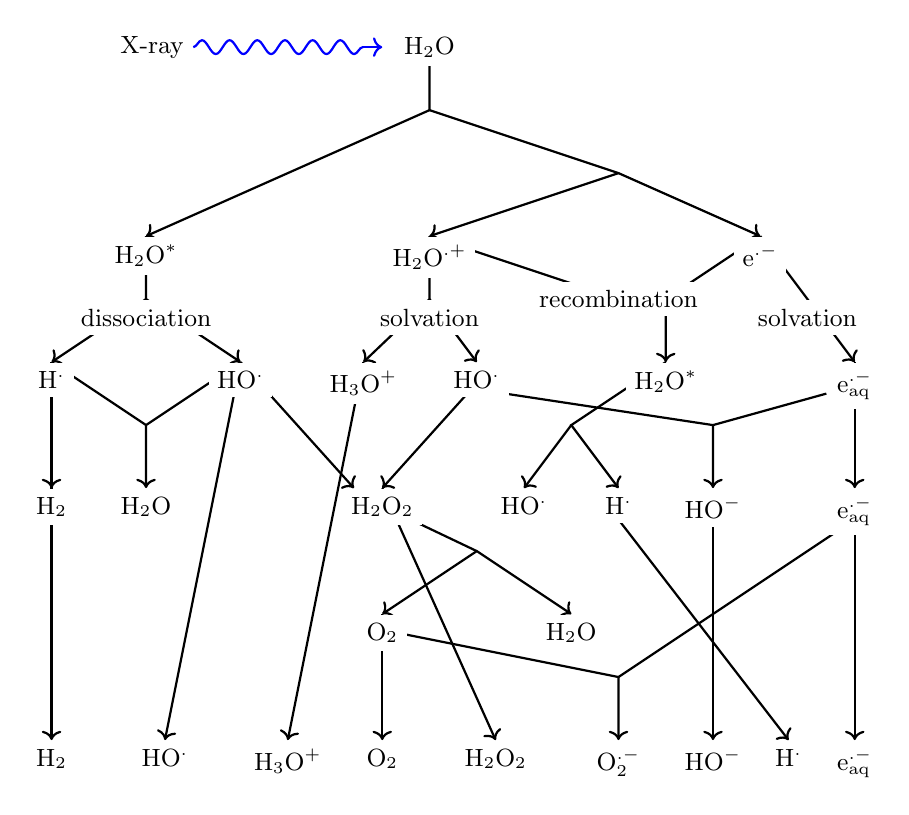
\begin{tikzpicture}[thick,xscale=1.2,yscale=0.8]
    \tikzset{snake it/.style={decorate, decoration=snake}}
    \small
    \def\yy{1};
    \def\xx{1};
    % educts 3 %%%%%%%%%%%%%%%%%%%%%%%%%%%%%%%%%%%%%%%%%% 
    % molecular hydrogen
    \draw[->](-4*\xx,-4*\yy)--(-4*\xx,-10*\yy)
    node[below,fill=white!100]{\chemfig{H_2}};
    % hydroxide radical
    \draw[->](-2*\xx,-4*\yy)--(-2.8*\xx,-10*\yy)
    node[below,fill=white!100]{\chemfig{HO^{.}}};
    % hydronium
    \draw[->](-0.7*\xx,-4*\yy)--(-1.5*\xx,-10*\yy)
    node[below,fill=white!100]{\chemfig{H_3O^{+}}};
    % molecular oxygen
    \draw[->](-0.5*\xx,-8*\yy)--(-0.5*\xx,-10*\yy)
    node[below,fill=white!100]{\chemfig{O_2}};
    % hydrogen peroxide
    \draw[->]((-0.5*\xx,-6*\yy)--(0.7*\xx,-10*\yy)
    node[below,fill=white!100]{\chemfig{H_2O_2}};
    % superperoxide
    \draw[](4.5*\xx,-6.5*\yy)--(2*\xx,-9*\yy);
    \draw[->](-0.5*\xx,-8.25*\yy)--(2*\xx,-9*\yy)--(2*\xx,-10*\yy)
    node[below,fill=white!100]{\chemfig{O_2^{.-}}};
    % hydroxide ion
    \draw[->](3*\xx,-6.5*\yy)--(3*\xx,-10*\yy)
    node[below,fill=white!100]{\chemfig{HO^{-}}};
    % hydrogen
    \draw[->](2*\xx,-6.5*\yy)--(3.8*\xx,-10*\yy)
    node[below,fill=white!100]{\chemfig{H^{.}}};
    % solvated electron
    \draw[->](4.5*\xx,-6.5*\yy)--(4.5*\xx,-10*\yy)
    node[below,fill=white!100]{\chemfig{e_{aq}^{.-}}};
    % educts 2 %%%%%%%%%%%%%%%%%%%%%%%%%%%%%%%%%%%%%%%%%% 
    % water
    \draw[->](-0.2*\xx,-6.5*\yy)--(0.5*\xx,-7*\yy)--(1.5*\xx,-8*\yy)
    node[below,fill=white!100]{\chemfig{H_2O}};
    % molecular oxygen
    \draw[->](0.5*\xx,-7*\yy)--(-0.5*\xx,-8*\yy)
    node[below,fill=white!100]{\chemfig{O_2}};
    % educts 1 %%%%%%%%%%%%%%%%%%%%%%%%%%%%%%%%%%%%%%%%%% 
    % molecular hygrogen
    \draw[->](-4*\xx,-4*\yy)--++(0,-2*\yy)
    node[below,fill=white!100]{\chemfig{H_2}};
    % water
    \draw[](-4*\xx,-4*\yy)--(-3*\xx,-5*\yy);
    \draw[->](-2*\xx,-4*\yy)--(-3*\xx,-5*\yy)--(-3*\yy,-6*\yy)
    node[below,fill=white!100]{\chemfig{H_2O}};
    % solvated electron
    \draw[->](4.5*\xx,-4*\yy)--++(0,-2*\yy)
    node[below,fill=white!100]{\chemfig{e_{aq}^{.-}}};
    % hydrogen peroxide
    \draw[->](0.4*\xx,-4.5*\yy)--(-0.5*\xx,-6*\yy);
    \draw[->](-2*\xx,-4*\yy)--(-0.8*\xx,-6*\yy);
    \draw[](-0.5*\xx,-6*\yy)
    node[below,fill=white!100]{\chemfig{H_2O_2}};
    % hydroxide ion
    \draw[](4.2*\xx,-4.5*\yy)--(3*\xx,-5*\yy);
    \draw[->](0.8*\xx,-4.5*\yy)--(3*\xx,-5*\yy)--(3*\xx,-6*\yy)
    node[below,fill=white!100]{\chemfig{HO^{-}}};
    %%%%%%%%%%%%%%%%%%%%%%%%%%%%%%%%%%%%%%%%%%% 
    % second recombination
    \draw[->](2.5*\xx,-4*\yy)--(1.5*\xx,-5*\yy)--(2*\xx,-6*\yy)
    node[below,fill=white!100]{\chemfig{H^{.}}};
    \draw[->](1.5*\xx,-5*\yy)--(1*\xx,-6*\yy)
    node[below,fill=white!100]{\chemfig{HO^{.}}};
    % dissociation
    \draw[->](-3*\xx,-3*\yy)--++(-\xx,-\yy)
    node[below,fill=white!100]{\chemfig{H^{.}}};
    \draw[->](-3*\xx,-2*\yy)--++(0,-\yy)
    node[below,fill=white!100]{dissociation}--+(\xx,-\yy)
    node[below,fill=white!100]{\chemfig{HO^{.}}};
    % solvated electron
    \draw[->](3.5*\xx,-2*\yy)--++(0.5*\xx,-\yy)
    node[below,fill=white!100]{solvation}--+(0.5*\xx,-\yy)
    node[below,fill=white!100]{\chemfig{e_{aq}^{.-}}};
    % solvated hydroxyl
    \draw[->](0,-3*\yy)--+(0.5*\xx,-\yy)
    node[below,fill=white!100]{\chemfig{HO^{.}}};
    \draw[->](0,-2*\yy)--++(0,-\yy)
    node[below,fill=white!100]{solvation}--+(-0.7*\xx,-\yy)
    node[below,fill=white!100]{\chemfig{H_3O^{+}}};
    % recombination
    \draw[->](3.5*\xx,-2*\yy)--++(-\xx,-\yy)--+(0,-\yy)
    node[below,fill=white!100]{\chemfig{H_2O^{*}}};
    \draw[-](0*\xx,-2*\yy)--++(2*\xx,-\yy)
    node[fill=white!100]{recombination};
    % primary products
    \draw[->](0,\yy)--(0,0)--(-3*\xx,-2*\yy)
    node[below,fill=white!100]{\chemfig{H_2O^{*}}};
    \draw[->](0,0)--(2*\xx,-\yy)--+(1.5*\xx,-\yy)
    node[below,fill=white!100]{\chemfig{e^{.-}}};
    \draw[->](2*\xx,-\yy)--+(-2*\xx,-\yy)
    node[below,fill=white!100]{\chemfig{H_2O^{.+}}};
    % water
    \draw[](0,\yy) node[fill=white!100]{\chemfig{H_2O}};
    % photon
    \path[yshift=\yy cm,draw=blue,snake it]
    (-2.5,0)node[left]{X-ray}--(-0.7,0);
    \draw[yshift=\yy cm,->,blue](-0.7,0)--(-0.5,0);
  \end{tikzpicture}
  \caption[Radiolysis of intracellular water.]{Radiolysis of
    (intracellular) water \protect\chemfig{H_2O}.  Exposure of cells
    to high-energetic ionising radiation induces the radiolysis of
    water molecules into hydronium \protect\chemfig{H_3O^{+}},
    hydroxyl radicals \protect\chemfig{HO^{.}}, solvated electrons
    \protect\chemfig{e_{aq}^{.-}}, and elemental hydrogen
    \protect\chemfig{H^{.}}.  These radicals are themselves chemically
    reactive, and in turn recombine to produce a series of highly
    \acf{ros} such as superoxide \protect\chemfig{HO_2} and peroxide
    \protect\chemfig{H_2O_2}, inflicting oxidative damage to molecules
    within the cell \cite{Arena1987}. }
  \label{fig:radiolysis}
\end{figure}
%%%%%%%%%%%%%%%%%%%%%%%%%%%%%%%%%%%%%%%%%%%%%%%%%%%%%%%%%%%%%%%%%%%%%%

% Water chemistry: Both the harmful effects of radiation upon
% biological systems (induction of cancer and acute radiation
% injuries) and the useful effects of radiotherapy involve the
% radiation chemistry of water. The vast majority of biological
% molecules are present in an aqueous medium; when water is exposed to
% radiation, the water absorbs energy, and as a result forms
% chemically reactive species that can interact with dissolved
% substances (solutes). Water is ionized to form a solvated electron
% and H2O+, the H2O+ cation can react with water to form a hydrated
% proton (H3O+) and a hydroxyl radical (HO.). Furthermore, the
% solvated electron can recombine with the H2O+ cation to form an
% excited state of the water, this excited state then decomposes to
% species such as hydroxyl radicals (HO.), hydrogen atoms (H.) and
% oxygen atoms (O.). Finally, the solvated electron can react with
% solutes such as solvated protons or oxygen molecules to form
% respectively hydrogen atoms and dioxygen radical anions. The fact
% that oxygen changes the radiation chemistry might be one reason why
% oxygenated tissues are more sensitive to irradiation than the
% deoxygenated tissue at the centre of a tumor. The free radicals,
% such as the hydroxyl radical, chemically modify biomolecules such as
% DNA, leading to damage such as breaks in the DNA strands. Some
% substances can protect against radiation-induced damage by reacting
% with the reactive species generated by the irradiation of the water.
% It is important to note that the reactive species generated by the
% radiation can take part in following reactions.

Of main concern in \ac{xpct} experiments involving biological samples
is the radiation induced damage of \ac{dna}, mediated by \acf{ros} and
overlapping with that caused by endogenous oxidative stress.  \ac{ros}
are produced by the radiolysis of cellular water.  Radiolysis is the
dissociation of molecules or atoms by highly energetic radiation into
smaller particles such as atoms, ions, or radicals.  When exposed to
radiation, water molecules become ionised or excited and subsequently
decompose in a series of energy transfer processes into both oxidising
and reducing species as illustrated in \cref{fig:radiolysis}
\cite{Gerschman1954a,Gerschman1954b,Hamill1969,Arena1987,LaVerne2000,Wren2010}.
In the case an electron is expelled from a water molecule upon
irradiation the primary ionic species produced are \chemfig{H_2O^{+}}
and \chemfig{e^{.-}}.  In aqueous solution the ionic species
convert into their hydrated entities: hydronium (hydrated proton)
\chemfig{H_3O^{+}}, the electrically neutral hydroxyl radical
\chemfig{HO^{.}}, and the solvated electron \chemfig{e_{aq}^{.-}}.  An
excited state of water may be formed directly by radiation or by the
recombination of \chemfig{H_2O^{+}} and \chemfig{e^{.-}}.  The excited
water molecule \chemfig{H_2^{*}} then dissociates into an elemental
hydrogen radical \chemfig{H^{.}} and a hydroxyl radical
\chemfig{HO^{.}}.  The reactive radical species may further recombine
to from stable products such as molecular \chemfig{H_2}, molecular
\chemfig{O_2}, \chemfig{H_2O}, or hydrogen peroxide \chemfig{H_2O_2}.
The solvated electron \chemfig{e_{aq}^{.-}} may further react with
oxygen to form superoxide (or hyperoxide) radicals \chemfig{O_2^{.-}}.
The relative concentrations of \chemfig{H_3O^{+}}, \chemfig{HO^{.}},
\chemfig{H_2O_2}, \chemfig{O_2}, \chemfig{H_2}, \chemfig{H^{.}},
\chemfig{O_2^{.-}}, and \chemfig{e_{aq}^{.-}} change considerably
within a short time scale following the initial interaction
\cite{Wren2010}.

% (diatomic) anionic hydroxide \chemfig{OH^{-}}
% hydrogen cation \chemfig{H^{+}}

The oxygen-oxygen bond in peroxides \chemfig{O_2^{.2-}} is unstable
and easily splits into other reactive radicals via homolytic cleavage.
Superoxides are potent oxidants implicating in cellular damage and
deleterious effects to tissues
\cite{Forest1999}. %active oxygen species
Hydrogen peroxide (\chemfig{H_2O_2}), formed in human and animal
organisms as a short-lived byproduct in biochemical processes, is
toxic to cells due to the oxidation of proteins, membrane lipids, and
\ac{dna} by the peroxide ion \cite{Loeffler2003}.  The superoxide
anion \chemfig{O_2^{.-}} and its protonated form, the hydroperoxyl (or
perhydroxyl) radical \chemfig{HO_2^{.}}, are in equilibrium in aqueous
solution.  Hydroperoxyl acts as an oxidant in biologically reactions
and is an initiator of lipid peroxidation.  Lipid peroxidation is the
oxidative degradation of lipids in cell membranes (loss of electron by
free radicals), resulting in cell damage.  Superoxide potentially
contributes to the pathogenesis of many diseases by means of 
oxidative damage it is inflicting on cells.  In nearly all organisms
living exposed to oxygen, the class of superoxide-scavenging enzymes,
called \ac{sod}, is developed as important antioxidant agents.
\ac{sod} serves an extremely efficient enzyme, since it catalyses the
neutralisation of superoxide almost as fast as the particles can meet
by diffusion in a solution.  \ac{sod} promotes the disproportionation
of superoxide into oxygen and hydrogen peroxide which can be further
degraded by the enzyme catalase into oxygen and water
\cite{Loeffler2003}.

To examine the pathogenic processes inflicted by radiation-induced
oxidative stress, one may consider biomarkers as  \ac{ros} itself
(direct detection), products of lipid peroxidation,
hydroxylated proteins, \ac{dna} base damage, or \ac{dna} strand
breaks.

%%%%%%%%%%%%%%%%%%%%%%%%%%%%%%%%%%%%%%%%%%%%%%%%%%%%%%%%%%%%%%%%%%%%%%
\begin{figure}
  \centering
  \includegraphics[width=0.99\textwidth]
{figures/NatProtoc/EmbryonicDissolution_ProjectionAndVolumeSlices.png}
\caption[Correspondence between radiographs and central-horizontal
slices of reconstructed tomograms, and disintegration of embryonic
compound.]{% Modified.
  Correspondence between radiographs and central-horizontal slices of
  reconstructed tomograms showing disintegration of embryo.  a-c,
  Radiographs of the same embryo at the same tomographic angle and for
  progressive points in time.  Intensity contrast is increasingly
  diminished due to tissue dissolution.  d-f, Central-horizontal
  slices through reconstructed volumes corresponding to (a-c),
  illustrating tissue damage.  Image adopted from
  \cite{Moosmann2014natp}.}
  \label{fig:disintegration}
\end{figure}
%%%%%%%%%%%%%%%%%%%%%%%%%%%%%%%%%%%%%%%%%%%%%%%%%%%%%%%%%%%%%%%%%%%%%%
Radiolysis of water eventually results in the accumulation of lethal
concentrations of radicals \cite{Kueltz2005}.  These radicals damage
both nucleic acids and native protein structures resulting in sudden
disintegration of tissue structure as depicted in
\cref{fig:disintegration} (see also \cite{Moosmann2013nature}).  As
damage to genes is likely to result in altered or loss of protein
function whenever and wherever those genes are expressed, we expect
damage inflicted on \acs{dna}/\ac{rna} to affect embryo viability more
severely than directly denatured proteins.


%%%%%%%%%%%%%%%%%%%%%%%%%%%%%%%%%%%%%%%%%%%%%%%%%%%%%%%%%%%%%%%%%%%%%%
%%%%%%%%%%%%%%%%%%%%%%%%%%%%%%%%%%%%%%%%%%%%%%%%%%%%%%%%%%%%%%%%%%%%%%

\section{Method}
\label{sec:method-optimisation}

A significant, universal understanding of cloning and crucial
developmental processes such as gastrulation or neurulation has been
gained by analysing Xenopus embryos
\cite{Gurdon1962a,Gurdon1962b,Keller2003}.  However, because its
embryos are optically opaque, the Xenopus model system has been
lacking high-resolution imaging techniques for the observation of cell
and tissue movements within the intact living embryo.  In Xenopus
embryos yolk is not limited to a yolk sac or a specified region of the
egg/embryo, but evenly distributed in the form of small yolk platelets
throughout the egg/embryo, rendering it opaque to visible light.  To
address this limitation, time-lapse in vivo \ac{xpct} was applied
(\cref{fig:setup}) to developing Xenopus embryos, which enables
imaging deep inside the embryos \cite{Moosmann2013nature}.

In vivo imaging of Xenopus embryos employing \ac{xpct} involves the
following stages.  The preparation of the embryo \cite{Kashef2009},
including in vitro fertilisation, embryo culturing, incubation,
staging, and suspension apt for X-ray tomographic imaging.  The
adjustment of the beamline setup, including choice of energy and
monochromaticity, adjustment of slits to reduce stray radiation,
alignment of the rotation axis, synchronisation of camera and fast
shutter (if used), focusing of microscope optics in the case of an
indirect detector system, and so forth.  The actual tomography in a
synchrotron beam, involving sample mounting, tomographic acquisition
with an appropriate choice of imaging parameters (see
\cref{sec:optimisation}), and immediate phase retrieval and
tomographic reconstruction to judge embryo vitality.  Subsequent data
analysis aims at time-resolved rendering and segmentation of
interesting structures and computation of velocity fields using
optical flow methods.  The derived velocity fields permit to visualise
the overall cell and tissues dynamics, the tracking of cells and
tissues via flow-field integration, and to distinguish active from
passive migration  via differential flow.  The latter
separates collective from  individual cell motion and thus
provides insight into the underlying propulsion mechanisms (convergent
extension, epiboly, collective cell migration on bulk tissue, etc.).


\subsection{Comparison with other methods}
\label{sec:comparison}

%%%%%%%%%%%%%%%%%%%%%%%%%%%%%%%%%%%%%%%%%%%%%%%%%%%%%%%%%%%%%%%%%%%%%%
\begingroup
\sloppy
\begin{table}
  \footnotesize
  \begin{tabu}
    { X[1.5,l] X[0.7c] X[0.9c] X[0.8c] X[1c] X[1.4c] X[1.85c]}
     4D in vivo imaging modality
    &  time lapse 
    &  spatial resolution
    &  time per tomogram
    &  struc\-tural information
    &  fluorescent labelling / contrast agents
    &  penetration depth for opaque embryos\\
    \hline
    \acs{mmri}       & $>$\SI{24}{h}  & $\sim$\SI{25}{\micro m}& $\sim$\SI{1}{h} & dense & optional &  whole embryo \\
confocal / light-sheet & $>$\SI{24}{h}  & $\sim$\SI{1}{\micro m} & $\sim$\SI{5}{s} & sparse&  yes     & surface, $\sim$2-3 cell layers \\
    \acs{xpct}        & $\sim$\SI{2}{h}& $\sim$\SI{1}{\micro m} & $\sim$\SI{20}{s}& dense &  no      & whole embryo \\  
  \end{tabu}
  \caption[Comparison of  four-dimensional in vivo imaging modalities in developmental biology.]
  {Comparison of  four-dimensional (4D) in vivo imaging modalities in developmental biology.}  
  \label{tab:imaging-modalities}
\end{table}
\endgroup
%%%%%%%%%%%%%%%%%%%%%%%%%%%%%%%%%%%%%%%%%%%%%%%%%%%%%%%%%%%%%%%%%%%%%%
% Modified
Using confocal light microscopy \cite{Ruffins2002} or digital scanned
light-sheet microscopy \cite{Huisken2004,Keller2008} permits to image
developmental processes in vivo at a spatio-temporal resolution
comparable to \ac{xpct}, but for longer periods.  However, their full
four-dimensional potential is realised only with optically translucent
embryos such as zebrafish and medaka and requires fluorescent
labelling of selected subcellular structures.  Moreover, only sparse
structural information is provided in the sense that only isolated
labelled parts contribute to the signal.  In contrast, in vivo
\ac{mmri} yields dense structural information throughout the whole and
optically opaque embryo (\eg{} mice and Xenopus) while maintaining
long time-lapse series \cite{Papan2006,Papan2007,Papan2007b}.
However, this imaging modality is currently limited to a spatial
resolution of about \SI{25}{\micro m}, and thus cannot resolve
subcellular structures.  Moreover, \ac{mmri} may require the use of
contrast agents in order to trace morphogenetic movements.
\Cref{tab:imaging-modalities} compares imaging parameters of
four-dimensional in vivo imaging modalities in developmental biology.

\subsection{Experimental setup}
\label{sec:setup}

In the following we exemplarily discuss in vivo scans which were
performed with bending-magnet beamline station 2-BM-B of \ac{aps} at
Argonne National Laboratory using a parallel X-ray beam of energy
$E=\SI{30}{keV}$ at a bandwidth of $\frac{\Delta E}{E} = \num{e-2}$
due to a double-multilayer monochromator.  In vivo scans were also
successfully conducted with undulator beamlines 32-ID at \ac{aps} and
ID19 at \ac{esrf}.  Other X-ray microtomography beamlines of similar
characteristics at third-generation synchrotron facilities can be used
as well.  The crucial parameters to be considered are a high flux
density at $E\approx\SI{30}{keV}$ and a bandwidth of $\frac{\Delta
  E}{E}<\num{e-2}$, a fast detector system, which, in combination,
permit to acquire tomograms within about \SI{30}{s}; moreover, a
sufficient coherence length at sample position, determined by the
source size and source-sample distance (see \cref{sec:coherence}),
which allows to benefit from a strongly enhanced intensity signal at
large propagation distance (\SIrange{1}{2}{m}) without loosing spatial
resolution due to source blurring.  The experimental setup is
illustrated in \cref{fig:setup}.  The choice of an X-ray energy of
$E\approx\SI{30}{keV}$ is influenced by two factors.

First is the fact that the attenuation length of X-rays in water
exhibits a strong power-law dependence on $E$.  \Eg{} X-rays at
\SI{30}{keV} impinging centrally on the cylindrical sample container
with a diameter of \SI{1.2}{cm} are attenuated upon exit
to about \SI{68}{\percent} of their incident intensity.  For lower
energies and given the short exposure time of \SIrange{15}{20}{ms},
imposed by the requirements on embryo viability and the necessity to
prevent motion blurring, the transmission decreases to values where
the signal-to-noise ratio is unacceptable.  

Secondly, the observation that embryo viability is unsatisfactory at
lower energies.  At $E = \SI{20.33}{keV}$  embryos started to
disintegrate (\cref{fig:disintegration}) already after a few (1-3)
tomograms.  Again, this is induced by the strongly increasing
absorption of X-rays with decreasing $E$ and the thus increased
deposition of X-ray dose.  

The emission spectrum of the bending magnet at beamline 2-BM peaks at
an energy of $E = \SI{17}{keV}$.  The spectral emission at $E
=\SI{30}{keV}$ is reduced by \SI{17}{\percent} with respect to the peak
at \SI{17}{keV}.  With a transverse size of the X-ray beam of
$\num{2}\times\SI{1.5}{mm^2}$, the photon flux density on the sample
is approximately \SI{e12}{photons/s/mm^2}.

A cylindrical polypropylene (Eppendorf) tube of radius $r =\SI{6}{mm}$
and height $h = \SI{3}{cm}$ serves as a sample container.  The embryo
is immersed in a buffer (nutrient) solution and suspended by the walls
of a hollow agarose cone within that container.  The tube is then
mounted on a standard tomography stage.

Intensity contrast, generated upon free-space propagation of X-rays
transmitted by the sample container, is recorded by a detector system
positioned at sample-detector distance of $z = \SI{62}{cm}$.  Within a
LuAg:Ce scintillator of \SI{100}{\micro m} thickness, X-ray photons
are converted into visible light.  After being reflected by a mirror,
the visible light is magnified by an optical microscope, placed at a
\SI{90}{\degree} angular offset with respect to the optical axis of
the X-ray beam (\cref{fig:setup}).  The microscope optic consists of a
Mitutoyo long working distance x5 lens.  The magnified light is then
detected within a pco.dimax \ac{cmos} camera with
$\num{2016}\times\num{2016}$ pixels of size
$\num{11}\times\SI{11}{\micro m^2}$.  This yields an effective pixel
size of $\Delta x =\SI{2.2}{\micro m}$.  The temperature in the
experimental hutch was about $\SI{25}{\degree.C}$, compatible with
natural conditions of development.  A significant rise of the sample
temperature due to heat load by X-ray absorption was excluded in
\cref{sec:bio-dose-heat}.


\subsection[\texorpdfstring{Optimisation of phase-contrast\\
  tomography setup}{Optimisation of phase-contrast tomography
  setup}]{Optimisation of phase-contrast tomography setup}
\label{sec:optimisation}

For propagation-based phase-contrast imaging, the detected intensity
contrast enhances when the sample-to-detector distance $z$ is
increased, see \cref{fig:fringe-evolution,fig:qp-2}(a).  Owing to
severe constraints on exposure times, imposed by the requirements on
embryo viability, the near-field condition
\begin{equation}
  \label{eq:near-field-condition}
  z \ll 4 \frac{(\Delta x)^2}{\lambda} \;,
\end{equation}
nominally required for phase retrieval within the edge-enhancement
regime \cref{eq:linear-tie-phase}, is deliberately violated for the
benefit of increased contrast.  Edge-enhancing fringes of transverse
extent $\lambda z$, representing object information, are not resolved
within this regime (\cref{fig:fringe-evolution}), but become visible
at sufficiently large $z$ as they are resolved
(\cref{fig:fringe-evolution}) and intensity contrast dominates noise
(\cref{fig:qp-2}(a)).

The propagation distance $z$ can be increased only up to a point where
the blurring of the detected image substantially affects the spatial
resolution, \ie{} where the blur $b$ is comparable to the effective
pixel size, see \cref{eq:source-blur}.  This blurring is due to the
finite extent of the X-ray source and a limited source-sample distance
$R$, see \cref{sec:coherence}.

At 2-BM-B, where $R\sim\SI{50}{m}$, a good compromise between enhanced
intensity signal and image blurring is given at $z = \SI{62}{cm}$.
The Van-Cittert-Zernike theorem for an incoherently emitting source of
a horizontal size $s\hon{v}\approx\SI{220}{\micro m}$ yields an
estimate for the horizontal blur of $b\ho{h}=\SI{3.4}{\micro m}$.
This is well below the resolution limit of $\sim 2 \Delta x =
\num{2}\times\SI{2.2}{\micro m} = \SI{4.4}{\micro m}$ imposed by the
Nyquist–Shannon sampling theorem \cite{Nyquist1928,Shannon1949}.  The
vertical source size of a synchrotron beam is usually much smaller
than its horizontal extend and thus not a limiting factor.

Tomographic projections were acquired under continuous rotation of the
sample (on the fly).  A number of $N = \num{1200}$ projections over
\SI{180}{\degree} were taken with a negligible read-out time of the
camera.  The value of $N$ is determined from the requirement that the
peripheral resolution at the object boundary is greater than the
effective pixel size $\Delta x$ of the detector.  From
\cref{eq:num-proj} we have $N\ge\tfrac{\pi}{2}N_x$, where $N_x$
denotes the horizontal number of effective pixels across the embryo's
diameter of $\sim\SI{1.2}{mm}$.

Measurements were taken at an X-ray energy of $E = \SI{30}{keV}$,
adjusted according to the two following considerations.  First, at
$E\sim\num{20},\SI{25}{keV}$ embryo viability was merely sufficient
for a few tomograms, covering a small window of the embryonic
development only.  Again, this is explained by the imaginary part
$\beta$ of the refractive index $n_\omega = 1 - \delta_\omega +
\ii\beta$ falling off with increasing energy.  Recall that, away from
absorption edges, this fall-off is faster than that of the real
decrement $\delta_\omega$, see \cref{fig:refractive-index}.

Secondly, photon flux density, scintillator absorption efficiency, and
$\delta_\omega$, which phase-contrast imaging is based upon, rapidly
decay with increasing energies.  In order to yield an acceptable
signal-to-noise ratio well above \SI{30}{keV} would require exposure
times too long to capture the movement of cells and tissues.  By
moving from $E = \SIrange{20}{30}{keV}$, photon flux density
\cite{Henke1993}, scintillator efficiency \cite{Martin2009}, and the
real refractive index decrement of water
$\delta_\omega(\chemfig{H_2O})$ (\cref{fig:refractive-index}) drop by
\SI{15}{\percent}, \SI{20}{\percent}, and \SI{50}{\percent},
respectively.  This trend continues more severely for X-ray energies
$E > \SI{30}{keV}$.  Typical cell velocities during Xenopus
gastrulation are in the order of $\sim\SI{2}{\micro m/min}$.  At an
effective pixel size of \SI{2.2}{\micro m}, this requires a full
tomogram to be recorded within less than $\SI{1}{min}$.  For energies
well above \SI{30}{keV}, acceptable signal-to-noise ratios would
require tomographic scan times of $>\SI{1}{min}$ because of the drops
in photon flux density and scintillator efficiency.  At \SI{30}{keV},
an effective pixel size of \SI{2.2}{\micro m}, and an exposure per
projection of \SI{15}{ms}, shot noise in the incoming beam is about
$\SI{0.4}{\percent}$.  Accounting for absorption in the sample
suspension system and scintillator efficiency, shot noise remains
acceptably low at about $\SI{1.8}{\percent}$.  However, read-out noise
owing to the dark current of the camera becomes significant at low
count rates.

Another means to reduce dose is to employ a fast shutter in order to
avoid the sample to be exposed to X-rays in between image acquisition.
However, this imposes additional constraints on available imaging
parameters (spatial resolution, exposure time, total scan time, etc.).
This is due to limitations caused by operating the shutter involving
minimum and maximum length of an open-close cycle, minimum and maximum
cycle rate, time needed to open and close the shutter (open and close
flank of the shutter blade), size of the shutter aperture potentially
obstructing the field of view, and so forth.

A waiting time of \SI{10}{min} between consecutive tomograms is
determined from the requirement that a typical endodermal cell of
$\sim\SI{40}{\micro m}$ diameter should not move more than
approximately half its diameter in between the acquisition of
consecutive tomograms.  Such a displacement is acceptable for the
computation of smooth velocity fields by means of optical flow
methods.


%%%%%%%%%%%%%%%%%%%%%%%%%%%%%%%%%%%%%%%%%%%%%%%%%%%%%%%%%%%%%%%%%%%%%%
%%%%%%%%%%%%%%%%%%%%%%%%%%%%%%%%%%%%%%%%%%%%%%%%%%%%%%%%%%%%%%%%%%%%%%

%%%%%%%%%%%%%%%%%%%%%%%%%%%%%%%%%%%%%%%%%%%%%%%%%%%%%%%%%%%%%%%%%%%%%%
\begin{figure}
  \centering
  \includegraphics[width=0.99\textwidth]{figures/Nature/Fig-2.jpg}
  \caption[3D time-lapse series visualising structure and dynamics of
  Xenopus laevis embryo during mid-gastrulation.]{% Modified.
    Three-dimensional time-lapse series visualising structure and
    dynamics of a Xenopus laevis embryo during mid-gastrulation. a-f,
    Renderings of mid-sagittally (a-c) and mid-horizontally (d-f)
    halved embryo at stages 11.5 (\SI{0}{min}), 12 (\SI{62}{min}) and
    12.5 (\SI{114}{min}).  Blue indicates ectoderm, orange mesoderm,
    and green endoderm.  g-i, Velocity fields $\vecv$ on a
    three-dimensional slab of \SI{180}{\micro m} thickness and centred
    about the cutting planes of (a-c).  For details on optical flow
    analysis see \cite{Moosmann2013nature,Moosmann2014natp}.  Colour
    bar indicates velocity magnitude representation.  Animal pole
    (AP), Archenteron (ARC), Brachet's cleft (BC), blastocoel (BLC),
    blastocoel floor (BLCF), blastocoel roof (BLCR), blastopore (BP),
    dorsal and ventral sides (D, V), dorsal and ventral blastopore lip
    (DBL, VBL), 'pipe' system within the interstitial tissue
    in-between archenteron and blastocoel (PS), ventral animal pole
    (VAP) and vegetal pole (VP).  Migration of mesendodermal tissue on
    the blastocoel roof is indicated by the red arrowhead in (g).
    Image adopted from \cite{Moosmann2013nature}.}
  \label{fig:bio-2}
\end{figure}
%%%%%%%%%%%%%%%%%%%%%%%%%%%%%%%%%%%%%%%%%%%%%%%%%%%%%%%%%%%%%%%%%%%%%%

\section{\texorpdfstring{Gastrulation in Xenopus laevis live cell imaging}{Gastrulation in Xenopus laevis live cell imaging}}
\label{sec:results}

%%%%%%%%%%%%%%%%%%%%%%%%%%%%%%%%%%%%%%%%%%%%%%%%%%%%%%%%%%%%%%%%%%%%%%
\begin{figure}
  \centering
  \includegraphics[width=0.99\textwidth]{figures/Nature/Fig-3.jpg}
  \caption[Cavity morphogenesis and quantitative assessment of
  morphological changes.]{% Modified
    Cavity morphogenesis and quantitative assessment of morphological
    changes.  a,b, Three-dimensional renderings of cavities of the
    archenteron (ARC), the blastocoel (BLC), and the 'pipe' system
    (PS) within the interstitial tissue in-between ARC and BLC for
    times \SI{62}{min} and \SI{114}{min}.  c, Volume change of ARC,
    BLC, and gastrula (entire embryo) from \SI{52}{min} to
    \SI{114}{min}.  Although the archenteron inflated, the blastocoel
    volume remained constant, whereas the volumes of the 'pipe' system
    and the entire embryo increased.  This indicates that early
    archenteron expansion is driven by the uptake of external water
    \cite{Tuft1962}.  Image adopted from \cite{Moosmann2014natp}.  }
  \label{fig:bio-3}
\end{figure}
%%%%%%%%%%%%%%%%%%%%%%%%%%%%%%%%%%%%%%%%%%%%%%%%%%%%%%%%%%%%%%%%%%%%%%

The discussion in the following is adopted from
\cite{Moosmann2013nature}.  At an X-ray energy of about \SI{30}{keV},
the experimental setup was configured to minimise dose while
sufficient image contrast is maintained according to
\cref{sec:optimisation}.  In \cref{sec:bio-dose-heat} heat load was
found to be negligible.  Radiolysis of water eventually leads to the
accumulation of lethal concentrations of radicals, resulting in a
sudden disintegration of tissue structure, see
\cref{sec:bio-dose-radio} and \cref{fig:disintegration}.  However,
before the onset of apoptosis, embryonic viability and morphogenetic
processes appear to be unimpaired.  Being an easily disrupted
developmental process, the closure of the blastopore was examined for
a direct assay of embryo viability.  Closure rates in X-rayed embryos
were found to be comparable with that in control gastrulae which were
viewed by light microscopy \cite{Moosmann2013nature}.  Time-lapse in
vivo sequences under various irradiation conditions, even harsher than
those described in \cref{sec:optimisation}, were acquired
\cite{Moosmann2013Xenbase,Moosmann2013nature}, confirming normal
development in X-rayed embryos.

\Cref{fig:bio-2}(a-c) depicts mid-sagittally halved renderings of an
embryo during mid-gastrulation at developmental stages 11.5, 12.0 and
12.5.  Specific embryonic structures can be identified, including the
blastopore, Brachet's cleft, archenteron, ventral and dorsal
blastopore lips, blastocoel, blastocoel roof and floor, and the
porous, interstitial tissue between archenteron and blastocoel (pipe
system).  Morphogenetic processes captured include the progression of
epiboly (spread of ectodermal cells) by a thinning of the ectoderm,
blastopore closure, and archenteron formation.  Further processes
captured are the crawling of cells on blastocoel floor, and in later
stages, the closing of the blastocoel, the closing of the neural tube,
and the migration of neural crest cells.  Further structures
identified in later stage are notochord, neural fold, prospective head
endoderm, neural plate, somitogenic mesoderm, lateral plate mesoderm,
endodermal yolk mass, eye anlage, brain anlage, remnants of the
blastocoel, and others \cite{Moosmann2013nature,Moosmann2013Xenbase}.

The time-lapse series of reconstructed volumes facilitate the analysis
of morphological changes and cell/tissue movements by means of
rendering, segmentation, and three-dimensional dense velocity fields
obtained from optical flow methods \cite{Brox2004}.  Optical flow
determines the displacement of a certain voxel in a given volume
towards the associated voxel in the consecutive volume such that the
difference in grey-values is minimised under certain constraints.
Morphogenesis is the collective consequence of hierarchical, diverse,
and coupled movements of cells and tissues.  All of these movements
can be captured by the velocity field $\vecv$.  The velocity fields
depicted in \cref{fig:bio-2}(g-i) reveal the collective movement of
cells within the gastrula for several morphogenetic processes.  This
includes the rotation of the vegetal endoderm (white arrowhead in
\cref{fig:bio-2}(g)) \cite{Winklbauer1999}, the involution of the
mesendoderm at the dorsal and ventral blastopore lip (white arrows in
\cref{fig:bio-2}(g)), and the migration of the mesendoderm on the
blastocoel roof towards the ventral animal pole (red arrowhead in
\cref{fig:bio-2}(g-i)) \cite{Keller2003}.

The Archenteron (or digestive tube) is the primordial gut that is
formed during gastrulation in the developing embryo.  The formation of
which is among the least understood aspects of gastrulation.  The
mid-horizontal slice of \cref{fig:bio-2}(e) depicts two distinct,
hollow regions (black arrows) which appear to be merged in
\cref{fig:bio-2}(f).  Renderings of the entire volume, shown in
\cref{fig:bio-3}(a,b), reveal a heart-shaped and contiguous
archenteron.  This highlights the importance of three-dimensional
imaging techniques.  The increased porosity of the 'pipe' system
within the interstitial tissue, as indicated by \cref{fig:bio-3}(a,b),
may suggest that the inflation of the archenteron is driven by fluid
transfer from the blastocoel via the 'pipe' system to the archenteron
\cite{Ewald2004}.  This hypothesis could be addressed upon a
segmentation of blastocoel, archenteron, cavities in the 'pipe'
system, and the entire embryo (gastrula) at different times
(\cref{fig:bio-3}(a-c)).  Although the archenteron inflated, the
blastocoel volume remained constant (\cref{fig:bio-3}(c)), whereas the
volumes of the 'pipe' system and the entire embryo increased.  Small
cavities within the blastopore disappear well before the inflation of
the archenteron and do not affect fluid balancing during the latter
\cite{Moosmann2013nature}.  This suggests early archenteron expansion
not to be driven by fluid transfer from the blastocoel
\cite{Ewald2004}, but instead by an uptake of external water
\cite{Tuft1962}.  The results concerning volume changes of the
archenteron, the 'pipe' system, and the entire embryo
(\cref{fig:bio-3}(a-c)), the conservation of cell-mass volume during
gastrulation \cite{Tuft1962}, and the absence of additional cavities
in the embryonic fluid balance \cite{Moosmann2013nature} affirm
archenteron inflation to be driven by the uptake of external water.


%%%%%%%%%%%%%%%%%%%%%%%%%%%%%%%%%%%%%%%%%%%%%%%%%%%%%%%%%%%%%%%%%%%%%%
\begin{figure}
  \centering
  \includegraphics[width=0.99\textwidth]{figures/Nature/Fig-4.jpg}
  \caption[Formation of a transient ectodermal ridge during
  confrontation of head and ventral mesendoderm.]{%Modified.
    Formation of a transient ectodermal ridge during confrontation of
    head and ventral mesendoderm.  a-e, Time-lapse sequence of
    sagittal slices through the confrontation zone at 52, 73, 83, 104
    and \SI{114}{min} showing the formation and relaxation of an
    ectodermal cusp on the blastocoel roof.  Dorsal and ventral
    leading edges (Dors-LE, Vent-LE), ectoderm (blue), mesoderm
    (orange), endoderm (green). f, Time-lapse sequence of shrinking
    contours starting at \SI{0}{min} (blue) and terminating at
    \SI{73}{min} within a rendering of the halved embryo at
    \SI{0}{min}.  The contour indicates projections of the migrating
    leading edge along the posterior-anterior axis onto the horizontal
    plane.  g, Three-dimensional rendering of individual cells, the
    ectodermal ridge, and cavities in-between in the confrontation
    zone at \SI{73}{min}.  Dors-LE cells (shades of green), Vent-LE
    cells (shades of red).  Image adopted from
    \cite{Moosmann2013nature}.}
  \label{fig:bio-4}
\end{figure}
%%%%%%%%%%%%%%%%%%%%%%%%%%%%%%%%%%%%%%%%%%%%%%%%%%%%%%%%%%%%%%%%%%%%%%

An interesting part of gastrulation is the active, non-invasive
migration of mesendodermal cells on their ectodermal substrate.  The
acquired time-lapse sequences capture, in detail, the migration of the
leading-edge head and ventral mesendoderm on the ectoderm of the
blastocoel roof (\cref{fig:bio-4}(f)).  The sagittal slices depicted
in \cref{fig:bio-4}(a-e) show regions of contact and non-contact
between the mesendoderm and the ectoderm, thereby creating cavities.
This is consistent with the model in \cite{Rohani2011} which proposes
that cell migration is driven by cycles of Eph/ephrin-dependent
attachment and repulsion.  Furthermore, a transient deformation of the
ectoderm towards the centre of the blastocoel is observed during the
migration of mesendodermal cells.  Namely, a cusp is formed in the
confrontation zone where the dorsal and ventral mesendoderm meet and
make contact (\cref{fig:bio-4}(b,c)).  The cusp shown in the sagittal
slices in \cref{fig:bio-4}(b,c) corresponds to a ridge in three
dimensions (\cref{fig:bio-4}(g)).  This ridge may be induced by a
local contraction of the ectoderm itself, or by a local, adhesive pull
of the confronting dorsal and ventral mesendoderm.  The spread of
ectodermal cells (epiboly) over the surface of the gastrula runs
opposite to the latter.  When dorsal and ventral mesendoderm
eventually overlap, their contact with the ectodermal substrate is
lost, the cusp relaxes (\cref{fig:bio-4}(c-e)), and new adhesive
interactions between mesendodermal cells from (\cref{fig:bio-4}(c)).
In explants, the formation of such a ridge is unlikely due to the
disruption of tissue tension.  To our knowledge this ridge has not
been reported before.

%%%%%%%%%%%%%%%%%%%%%%%%%%%%%%%%%%%%%%%%%%%%%%%%%%%%%%%%%%%%%%%%%%%%%%
%% CHAPTER
%%%%%%%%%%%%%%%%%%%%%%%%%%%%%%%%%%%%%%%%%%%%%%%%%%%%%%%%%%%%%%%%%%%%%%

\chapter{Summary  and Outlook}
\label{cha:summary}

In \cref{cha:intro} historical steps in the discovery of X-rays and
their immediate application for structure determination in material
science and for two- and three-dimensional imaging in life sciences
were recapitulated.  Significantly enhanced coherence and brilliance
of synchrotron radiation allow interference effects to arise upon beam
propagation and thus to exploit the elastic scattering of X-rays by
the sample via non-interferometric, propagation-based phase contrast.
There, the object information is encoded in the phase of the
transmitted and subsequently propagated wave field.  The ensuing
non-local and non-linear relation between propagated intensity and
exit phase evades an exact analytic inversion of the forward problem.
Thus, phase retrieval demands for an efficient approximation to
approach an adequate solution.  Owing to its simple instrumentation
and dose efficiency propagation-based phase contrast is apt for
high-resolution in vivo imaging.

In \cref{cha:theory,cha:exp} theoretical and experimental principles
of X-ray imaging were reviewed.  Microscopic interactions of X-rays
with matter were connected to an effective description in terms of the
macroscopic refractive index.  Using Fresnel theory, the interaction
of quasi\hyph parallel, monochromatic, hard X-rays with soft matter
inducing phase variations in the ensuing wave field, the subsequent
generation of intensity contrast upon forward propagation of the
transmitted wave front, and the effects of partial beam coherence
impairing emergent intensity contrast were described.  Linear methods
of phase retrieval based on the \acl{tie} and the \acl{ctf}, including
a phase-attenuation duality which accounts for absorptive effects at
large X-ray energies, were discussed in detail and tomographic
reconstruction from retrieved phase maps, restoring the sample's
electron density, was considered.

In \cref{cha:beyond} approaches to phase retrieval beyond linearity
were presented.  

In \cref{sec:perturbation-theory} a systematic extension of the linear
phase retrieval for the propagation-based technique was developed in
the case of pure\hyph phase objects (soft tissue, polymers, etc.).
Here, a model was proposed which expands intensity and phase of the
propagated wave field in powers of the object\hyph detector distance.
Appealing to full Fresnel theory, the expansion coefficients were
determined in terms of transverse derivatives acting on the phase at
object exit.  The ensuing partial differential equation exhibits
non-linear behaviour at next\hyph to\hyph leading order and was
approached in a perturbative fashion.

Apt to retrieve large phase variation over the entire field of view,
this method demonstrated promising results for simulated phantom data
of extended.  Large variations in the refractive index are averaged in
phase shifts accumulated along a ray path through a thick sample.  The
accumulate phase is thus less prone to small\hyph scale variations
within the projected object.  This facilitates to fulfil the
requirement of small values of transverse derivatives of the phase for
the expansion of the intensity contrast to converge.  The non-linear
perturbative approach is therefore expected to be applicable to the
tomography of samples introducing large phase shifts.  Employing
different basis sets than just powers in the propagation distance is
presumed to yield better convergence properties of the expansion.

\Cref{sec:qp} discussed the case where considerable variations of the
exit phase entail non-local and non-linear contrast transfer from exit
phase to propagated intensity.  Here, a phase-scaling symmetry, exact
in the limit of vanishing phase variations, was identified and
exploited in order to render contrast transfer quasi\hyph linear,
reminiscent to the concept of quasiparticles.  Algebraic and linear
phase retrieval then persists when using a mildly renormalised
intensity.

Noise in the retrieved phase, induced by a given integrated, shot\hyph
noised intensity at a single propagation distance, was analysed in the
case of ideal spatio-temporal coherence.  Phase noise was found to
decrease with the inverse propagation distance upon quasiparticle
retrieval.  For intensity contrast emerging upon free-space
propagation of considerable phase variations at object exit,
encountered \eg{} in \acl{xpct} of early stage model organisms,
quasiparticle phase retrieval serves as a powerful tool.  For ex vivo
imaging, superiority in resolution compared to conventional approaches
to single\hyph distance phase retrieval is demonstrated.  For in vivo
imaging, modified quasiparticle phase retrieval presently exhibits a
more modest improvement of resolution, though significantly superior
to the conventional modality.  The drastically enhanced coherence and
brilliance of X-ray beams, soon to be provided by various upgraded
third generation synchrotron radiation facilities, render imaging at
propagation distances in the tens of meters feasible, significantly
improving the intensity signal.  In vivo imaging under parallel\hyph
beam incidence and at a reasonable X-ray dose will then resolve with
spatial resolution at the detector limit.


%% TOMOGRAPHY
In \cref{cha:tomography} intricacies of tomography were discussed in
the context of phase\hyph contrast data.  Of main concern are
large\hyph scale modulations superimposed on the tomographic
reconstruction and thereby obscuring small-scale features of the
object under investigation and impairing subsequent data processing
and analysis.  These large\hyph scale modulations are caused by
absorptive contributions to the intensity, distorting low-frequency
components that are enhanced upon phase retrieval and local
tomography.  By reversing the order of phase retrieval and tomographic
reconstruction, the real refractive index decrement is directly
retrieved from the 'intensity volume', which significantly reduces
large-scale modulations compared to conventional processing order.
Moreover, propagated intensity data can then be used as input for
alternative (algebraic) tomographic reconstruction techniques
which would otherwise be impaired by large\hyph scale variations in
the retrieved phase maps.


%% NATURE 
In \cref{cha:bio}, using highly coherent synchrotron radiation in the
hard X-ray regime, high-resolution phase-contrast microtomography was
conceived as a three-dimensional in vivo imaging modality to
investigate early developmental processes in intact model\hyph system
embryos.  Here, low-dose requirements demand short exposure times
which calls for a single measurement at a large propagation distance.

Four-dimensional imaging of living early-stage vertebrate embryos
presently requires a minimum X-ray dose which limits maximum time\hyph
lapse series to about two\hyph hour duration and spatial resolution to
about $\SI{2}{\micro m}$ at propagation distance in the order of
$\SI{1}{m}$ \cite{Moosmann2013nature,Moosmann2014natp}.  Introducing a
moderate beam divergence to enable geometric magnification effectively
increases spatial resolution (Fresnel scaling \cite{PaganinBook}).
\acl{xpct} will then resolve in the hundred-nanometre regime with
commensurate or even longer periods of development due to a more
localised dose deposition.  On the instrumentation side, this will
require focusing optics for hard X-rays such as Kirkpatrick-Baez
mirrors \cite{Requena2009}, long beamline hutches, and vacuum tubes
downstream of the sample stage to prevent X-ray absorption by air
before detection.  Performing in vivo \acl{xpct} with such a setup
will contribute to a profound understanding of \eg{} developmental
processes by the comparison of phenotypic effects of molecular
perturbations at subcellular resolution and in four dimensions.

In particular, as demonstrated by the study in \cref{sec:results}, in
vivo propagation\hyph based, single\hyph distance X-ray phase\hyph
contrast microtomography combined with optical flow analysis serves as
a powerful tool to investigate the embryonic development in Xenopus
laevis in four dimensions.  Differential flow analysis enabled to
distinguish active from passive movement of cells and tissue,
elucidating how collective motion (convergent extension, collective
cell migration on bulk tissue, etc) is propelled by individual cell
behaviour.  At subcellular resolution, time-lapse series of up to two
hours of development could be captured without adverse effects on
embryo viability.  Using this imaging modality in high-throughput
perturbation experiments, can contribute to our understanding of the
molecular mechanisms and biomechanical processes driving
morphogenesis.


%%%%%%%%%%%%%%%%%%%%%%%%%%%%%%%%%%%%%%%%%%%%%%%%%%%%%%%%%%%%%%%%%%%%%%
%% END OF TEXT
%%%%%%%%%%%%%%%%%%%%%%%%%%%%%%%%%%%%%%%%%%%%%%%%%%%%%%%%%%%%%%%%%%%%%%

\appendix
\numberwithin{equation}{chapter}
\cleardoublepage
%\part{Appendix}
%********************************************************************
% Appendix
%*******************************************************
% If problems with the headers: get headings in appendix etc. right
\markboth{\spacedlowsmallcaps{Appendix}}
{\spacedlowsmallcaps{Appendix}}
\phantomsection 
\refstepcounter{dummy}


\chapter{Fourier analysis}
\label{cha:fourier-analysis}

\section{Definitions using angular frequencies}
\label{sec:fourier-k}

\subsection{Fourier transformation}
\label{sec:ft-k}

Consider a scalar function $f$ of a real $n$-dimensional variable
$\vecx=(x_1,x_2,\dots,x_n)$.  The $n$-dimensional Fourier transform of
the function $f$ is denoted $\ft{f}\equiv\F_\vecx f$ where $\F_\vecx$
is the forward Fourier transform operator.  The related inverse
Fourier transform operator is denoted $\iF_\veck$. The Fourier
variable conjugate to $\vecx$ is $\veck=(k_1,k_2,\dots,k_n)$.  The
operator $\F_{x_i}$ demands Fourier transformation with respect to the
argument $x_i$.  A vector index in $\F_\vecx$ or multiple indices in
$\F_{\{x_i\}}$ indicate multidimensional Fourier transformations with
respect to the set of variables $\{x_i\}$.  When no confusion can
arise, we will omit the indices of the Fourier transform operators.
The $n$-dimensional Fourier transform of the function $f$ is defined
as
\begin{equation}
  \label{eq:ft-k-n}
  \ft{f}(\veck) \equiv (\F_\vecx f)(\veck) \equiv
  \frac{1}{(2\pi)^{n/2}}\int_{-\infty}^\infty \Intd{^n\vecx} 
  f(\vecx) \expp{\ii\veck\cdot\vecx} 
\end{equation}
and the corresponding inverse Fourier transform as
\begin{equation}
  \label{eq:ift-k-n}
  f(\vecx) \equiv (\FO{^{-1}_\veck} \ft{f})(\vecx) \equiv
  \frac{1}{(2\pi)^{n/2}}\int_{-\infty}^\infty \Intd{^n\veck} 
  \ft{f}(\veck) \exp(-\ii\veck\cdot\vecx) \;.
\end{equation}
With the above definitions an expression for the $n$-dimensional Dirac
delta distribution is follows as
\begin{equation}
  \label{eq:dirac-k-n}
  \delta^n(\vecx) =
  \frac{1}{(2\pi)^n}\int_{-\infty}^\infty \Intd{^n\veck} 
   \exp(\ii\veck\cdot\vecx) \;.
\end{equation}
For non-zero scalar $\alpha$ the Dirac delta
distribution satisfies the scaling property
\begin{equation}
  \label{eq:dirac-scaling}
  \delta^n(\alpha\vecx)=\frac{\delta^n(\vecx)}{\abs{\alpha}^n} \;.
\end{equation}

For referencing we will give explicit expressions for $n=\{1,2,3\}$.
For $n=1$ and setting $x=x_1$ and $k=k_1$, we have
\begin{equation}
  \label{eq:ft-k-1}
  \begin{split}
      \ft{f}(k) &\equiv (\F_x f)(k) &\equiv
  \frac{1}{\sqrt{2\pi}}\int_{-\infty}^\infty \Intd{x} 
  f(x) \expp{\ii k x} \;, \\
  f(x) &\equiv (\FO{^{-1}_k} \ft{f})(x) &\equiv
  \frac{1}{\sqrt{2\pi}}\int_{-\infty}^\infty \Intd{k} 
  \ft{f}(k) \exp(-\ii k x) \;.
  \end{split}
\end{equation}
For $n=2$ and setting $\vecxp=(x_1,x_2)$ and $\veckp=(k_1,k_2)$, we
have
\begin{equation}
  \label{eq:ft-k-2}
  \begin{split}
    \ft{f}(\veckp) & \equiv (\F_{\vecxp} f)(\veckp) &\equiv
    \frac{1}{2\pi}\int_{-\infty}^\infty \Intdd{\vecxp} 
    f(\vecxp) \expp{\ii\veckp\cdot\vecxp} \;,
    \\   f(\vecxp) &\equiv (\FO{^{-1}_{\veckp}} \ft{f})(\vecxp) &\equiv
    \frac{1}{2\pi}\int_{-\infty}^\infty \Intdd{\veckp} 
    \ft{f}(\veckp) \exp(-\ii\veckp\cdot\vecxp) \;.
  \end{split}
\end{equation}
For $n=3$ and setting $\vecr=(x_1,x_2,x_3)$ and $\veck=(k_1,k_2,k_3)$,
we have
\begin{equation}
  \label{eq:ft-k-3}
  \begin{split}
    \ft{f}(\veck) &\equiv (\F_\vecr f)(\veck) &\equiv
    \frac{1}{(2\pi)^{3/2}}\int_{-\infty}^\infty\Intddd{\vecr}
    f(\vecr)\expp{\ii\veck\cdot\vecr} \;,
    \\  f(\vecr) &\equiv (\FO{^{-1}_\veck} \ft{f})(\vecr) &\equiv
  \frac{1}{(2\pi)^{3/2}}\int_{-\infty}^\infty \Intddd{\veck} 
  \ft{f}(\veck) \exp(-\ii\veck\cdot\vecr) \;.
  \end{split}
\end{equation}

\subsection{Convolution theorem}
\label{sec:convolution-k}

Let $\ast$ indicate (one-dimensional) convolution with respect to
coordinate $x_i$.  The $n$-dimensional convolution of scalar functions
$f$ and $g$ is defined as
\begin{equation}
  \label{eq:convolution-n}
  f(\vecx)\ast\ast\dots\ast g(\vecx) 
  = \int_{-\infty}^\infty\Intd{^n\vecx'}f(\vecx')g(\vecx-\vecx') \;.
\end{equation}
The convolution theorem in $n$-dimensional space using the Fourier
transform as defined in \cref{eq:ft-k-n} and \cref{eq:ift-k-n} reads
\begin{equation}
  \label{eq:convolution-theorem-k-n}
  \F_\vecx[f(\vecx)\ast\ast\dots\ast g(\vecx)] = 
  (2\pi)^n (\F_\vecx f) \times (\F_\vecx g) \;.
\end{equation}

\subsection{Fourier derivative theorem}
\label{sec:fourier-derivative-k-n}

Appealing to the Fourier representation of function $f$, the Fourier
derivative theorem reads
\begin{equation}
  \label{eq:fdt-k-n}
  \frac{\pd^m}{\pd x_i^m} f(\vecx) = 
    \FO{^{-1}_{k_i}}\lrb{ (-\ii k_i)^m \F_{x_i} f(\vecx) } \;,
\end{equation}
with $m\in\mathbb{N}_0$.

\section{Definitions using ordinary frequencies}
\label{sec:fourier-xi}

Here we will give expressions for the formulae of \cref{sec:fourier-k}
when using ordinary frequencies, $\vecxi=(\xi_1,\xi_2,\dots,\xi_n)$,
instead of angular frequencies $\veck$ with $\veck=2\pi\vecxi$.  The
advantage of defining the Fourier transform using ordinary instead of
angular frequencies is that factors $\frac{1}{(2\pi)^{n/2}}$ vanish in
\cref{eq:ft-xi-n} and \cref{eq:ift-xi-n} compared to the definitions
in \cref{eq:ft-k-n} and \cref{eq:ift-k-n}.  Moreover, the factor
$(2\pi)^{n/2}$ vanishes in the definition of the convolution theorem.
Furthermore, numerical implementations usually employ discretised
version of the Fourier transforms as defined below.

\subsection{Fourier transformation}
\label{sec:ft-xi}

The $n$-dimensional Fourier transform of the function $f$ using
ordinary frequencies $\vecxi$ is defined as
\begin{equation}
  \label{eq:ft-xi-n}
  \ft{f}(\vecxi) \equiv (\F_\vecx f)(\vecxi) \equiv
  \int_{-\infty}^\infty \Intd{^n\vecx} 
  f(\vecx) \expp{\ii2\pi\vecxi\cdot\vecx}
\end{equation}
and the corresponding inverse Fourier transform as
\begin{equation}
  \label{eq:ift-xi-n}
  f(\vecx) \equiv (\FO{^{-1}_\vecxi} \ft{f})(\vecx) \equiv
  \int_{-\infty}^\infty \Intd{^n\vecxi} 
  \ft{f}(\veck) \exp(-\ii2\pi\vecxi\cdot\vecx) \;.
\end{equation}
With the above definitions the $n$-dimensional Dirac
delta distribution reads
\begin{equation}
  \label{eq:dirac-xi-n}
  \delta^n(\vecx)  = 
  \int_{-\infty}^\infty \Intd{^n\vecxi} 
   \exp(\ii\vecxi\cdot\vecx) \;.
\end{equation}

\subsection{Convolution theorem}
\label{sec:convolution-xi}

The convolution theorem in $n$-dimensional space using the Fourier
transform as defined in \cref{eq:ft-xi-n} and \cref{eq:ift-xi-n} reads
\begin{equation}
  \label{eq:convolution-theorem-xi-n}
  \F_\vecx[f(\vecx)\ast\ast\dots\ast g(\vecx)] = 
  (\F_\vecx f) \times (\F_\vecx g) \;.
\end{equation}
For $n=2$ and setting $\vecxp=(x_1,x_2)$ we have
\begin{equation}
  \label{eq:convolution-theorem-xi}
    \F_{\vecxp}[f \conv g] = (\F_{\vecxp} f) \times (\F_{\vecxp} g) \;.
\end{equation}


\subsection{Fourier derivative theorem}
\label{sec:fourier-derivative-xi-n}

Appealing to \cref{eq:ift-xi-n} and \cref{eq:ft-xi-n}, the Fourier
derivative theorem reads
\begin{equation}
  \label{eq:fdt-xi-n}
  \frac{\pd^m}{\pd x_i^m} f(\vecx) = \F^{\operatorname{-1}}_{\xi_i}
  \lrb{ (-\ii2\pi \xi_i)^m \F_{x_i} f(\vecx) } \;,
\end{equation}
with $m\in\mathbb{N}_0$.

For referencing we will give explicit expressions for $n=\{1,2,3\}$.
For $n=1$ and setting $x=x_1$ and $\xi=\xi_1$, we have
\begin{equation}
  \label{eq:ft-xi-1}
  \begin{split}
    \ft{f}(\xi) &\equiv (\F_x f)(\xi) 
    \equiv{}& \int_{-\infty}^\infty \Intd{x} 
    f(x) \expp{\ii 2\pi \xi x} \;,
    \\ f(x) &\equiv (\F{^{\operatorname{-1}}_\xi} \ft{f})(\xi) \equiv{}&
    \int_{-\infty}^\infty \Intd{\xi} 
    \ft{f}(\xi) \exp(-\ii 2\pi\xi x) \;.
  \end{split}
\end{equation}
For $n=2$ and setting $\vecxp=(x_1,x_2)$ and $\vecxi=(\xi_1,\xi_2)$,
we have
\begin{equation}
  \label{eq:ft-xi-2}
  \begin{split}
    \ft{f}(\vecxip) &\equiv (\F_{\vecxp} f)(\vecxip) 
    \equiv{}&\int_{-\infty}^\infty \Intdd{\vecxp} 
  f(\vecxp) \expp{\ii 2\pi\vecxip\cdot\vecxp} \;,
  \\   f(\vecxp) &\equiv (\F{^{\operatorname{-1}}_{\vecxip}} \ft{f})(\vecxp)
  \equiv{}& \int_{-\infty}^\infty \Intdd{\vecxip} 
  \ft{f}(\veckp) \exp(-\ii2\pi\vecxip\cdot\vecxp) \;.
  \end{split}
\end{equation}
For $n=3$ and setting $\vecr=(x_1,x_2,x_3)$ and
$\vecxi=(\xi_1,\xi_2,\xi_3)$, we have
\begin{equation}
  \label{eq:ft-xi-3}
  \begin{split}
    \ft{f}(\vecxi) &\equiv (\F_\vecr f)(\vecxi) \equiv{}&
    \int_{-\infty}^\infty\Intddd{\vecr}
    f(\vecr)\expp{\ii 2\pi\vecxi\cdot\vecr} \;,
    \\ f(\vecr) &\equiv (\FO{^{-1}_\vecxi} \ft{f})(\vecr) \equiv{}&
    \int_{-\infty}^\infty \Intddd{\vecxi} 
    \ft{f}(\veck) \exp(-\ii 2\pi\vecxi\cdot\vecr) \;.
  \end{split}
\end{equation}

\cleardoublepage

%*******************************************************
% List of Figures and of the Tables
%*******************************************************
%\clearpage
\begingroup 
\let\clearpage\relax
\let\cleardoublepage\relax
\let\cleardoublepage\relax
    %*******************************************************
    % List of Figures
    %*******************************************************    
    \manualmark
    \markboth{\spacedlowsmallcaps{\listfigurename}}
    {\spacedlowsmallcaps{\listfigurename}}
    \phantomsection 
    \refstepcounter{dummy}
    \addtocontents{toc}{\protect\vspace{\beforebibskip}}
    \addcontentsline{toc}{chapter}{\tocEntry{\listfigurename}}

    \begingroup
    \raggedright
    \sloppy
    \listoffigures
    \endgroup
    
    %\listoffigures
    \vspace*{8ex}
    %*******************************************************
    % List of Tables
    %*******************************************************
    \manualmark
    \markboth{\spacedlowsmallcaps{\listtablename}}
    {\spacedlowsmallcaps{\listtablename}}
    \phantomsection 
    \refstepcounter{dummy}
    \addtocontents{toc}{\protect\vspace{\beforebibskip}}
    \addcontentsline{toc}{chapter}{\tocEntry{\listtablename}}
    \begingroup
    \raggedright
    \sloppy
    \listoftables        
    \endgroup
    \vspace*{8ex}
\endgroup 

%%%%%%%%%%%%%%%%%%%%%%%%%%%%%%%%%%%%%%%%%%%%%%%%%%%%%%%%%%%%%%%%%%%%%%
% Acronyms
%%%%%%%%%%%%%%%%%%%%%%%%%%%%%%%%%%%%%%%%%%%%%%%%%%%%%%%%%%%%%%%%%%%%%%
\chapter*{Acronyms}
\manualmark
\markboth{\spacedlowsmallcaps{Acronyms}}
{\spacedlowsmallcaps{Acronyms}}
\phantomsection 
\refstepcounter{dummy}
\addtocontents{toc}{\protect\vspace{\beforebibskip}}
\addcontentsline{toc}{chapter}{\tocEntry{Acronyms}}
%\pdfbookmark[1]{Acronyms}{acronyms}
\begin{acronym}
  \setlength{\itemsep}{-\parsep}% sorgt dafür, dass zwischen den
  % Einträgen kein Abstand ist und das Verzeichnis kompakt dargestellt
  % wird.
  \acro{anka}[ANKA]{Angströmquelle Karlsruhe}
  \acro{aps}[APS]{Advanced Photon Source}
  \acro{anl}[ANL]{Argonne National Laboratory}
  \acro{art}[ART]{algebraic reconstruction technique}
  \acro{bp}[BP]{backprojection}
  \acro{bm}[BM]{bending magnet}
  \acro{ccd}[CCD]{charge-coupled device}
  \acro{cgls}[CGLS]{conjugate gradient method for least squares}
  \acro{cmos}[CMOS]{complementary metal-oxide-semiconductor}
  \acro{ct}[CT]{computed tomography}
  \acro{ctf}[CTF]{contrast transfer function}
  \acro{dart}[DART]{discrete algebraic reconstruction technique}
  \acro{dcm}[DCM]{double crystal monochromator}
  \acro{DESY}{Deutsches Elektron-Synchrotron}
  \acro{dna}[DNA]{deoxyribonucleic acid}
  \acro{esrf}[ESRF]{European Synchrotron Radiation Facility}
  \acro{EXAFS}{extended X-ray absorption fine structure}
  \acro{fbp}[FBP]{filtered backprojection}
  \acro{FEL}{free-electron laser}
  \acro{fft}[FFT]{fast Fourier transform}
  \acro{fov}[FOV]{field of view}
  \acro{fwhm}[FWHM]{full width at half maximum} 
  \acro{gpu}[GPU]{graphics processing unit}
  \acro{id}[ID]{insertion device}
  \acro{ips}[IPS]{Institute for Photon Science and Synchrotron Radiation}
  \acro{mmri}[$\mu$MRI]{microscopic magnetic resonance imaging}
  \acro{na}[NA]{numerical aperture}
  \acro{nnfbp}[NN-FBP]{neural-network filtered backprojection}
  \acro{rna}[RNA]{ribonucleic acid}
  \acro{ros}[ROS]{reactive oxygen species}
  \acro{sart}[SART]{simultaneous algebraic reconstruction technique}
  \acro{sase}[SASE]{self-amplified spontaneous emission}
  \acro{sirt}[SIRT]{simultaneous iterative reconstruction technique}
  \acro{snr}[SNR]{signal-to-noise ratio}
  \acro{sod}[SOD]{superoxide dismutase}
  \acro{tie}[TIE]{transport-of-intensity equation}
  \acro{tft}[TFT]{thin-film transistor}
  \acro{XASF}{X-ray absorption fine structure}
  \acro{XANES}{X-ray absorption near-edge structure}
  \acro{XFEL}{X-ray free-electron laser}
  \acro{xpct}[XPC$\mu$T]{X-ray phase-contrast microtomography}
\end{acronym}
%\endgroup
\cleardoublepage

%********************************************************************
% Bibliography
%*******************************************************
\manualmark
 % work-around to have small caps also
\markboth{\spacedlowsmallcaps{\bibname}}{\spacedlowsmallcaps{\bibname}}
\phantomsection 
\refstepcounter{dummy}
\addtocontents{toc}{\protect\vspace{\beforebibskip}} % to have the bib
% a bit from the rest in the toc
\addcontentsline{toc}{chapter}{\tocEntry{\bibname}}
\label{app:bibliography} 
%\bibliographystyle{alpha}%unsrt,osajn
%\bibliographystyle{./custom-bib/phd-custom-bib}
%\bibliography{Bibliography}

% Use standard bibliography as above or biblatex with the following
% command. Then bibliographystyle has to be passed as option to
% biblatex!

\begingroup
\raggedright
\sloppy
\printbibliography
\endgroup
\cleardoublepage

%*******************************************************
% Acknowledgments
%*******************************************************
\begingroup
\let\clearpage\relax
\let\cleardoublepage\relax
\let\cleardoublepage\relax
\chapter*{Acknowledgements}
\thispagestyle{empty}
\pagestyle{empty}
\manualmark
\markboth{\spacedlowsmallcaps{Acknowledgements}}
{\spacedlowsmallcaps{Acknowledgements}}
\phantomsection 
\refstepcounter{dummy}
% \addtocontents{toc}{\protect\vspace{\beforebibskip}}
% \addcontentsline{toc}{chapter}{\tocEntry{Acknowledgements}}

\sloppy

First of all, I am very much indebted to my doctoral advisor PD
Dr. Ralf Hofmann.  His enduring support and encouragement were
essential on the way to my docorate.  I am very grateful for his
guidance, the many enlightening discussions, and his invaluable
theoretical input.  And also his support in a number of experiments at
\ac{aps} and \ac{esrf}.

I am also indebted to Professor Dr. Tilo Baumbach for the opportunity
to do my doctorate at the \ac{ips} / \ac{anka}.  I am very grateful
for his support and his scientific input.

Special thanks to Daniel Hänschke for his support in a number of
experiments at ANKA and ESRF, and the many discussions on 
theoretical and experimental aspects in imaging experiments and on
computational issues concerning data processing and handling.

 Special thanks to Venera Weinhardt for her support during a
number of experiments, her help on data processing and discussions on
imaging matters.

Special thanks to Jubin Kashef for providing first biological test
samples, his help during a number of experiments at APS and ESRF, and
his valuable input and insights regarding biological matters.

Special thanks also to Lukas Helfen for his great support and
commitment in numerous experiments at beamlines
ID15, ID19, and BM05 at \ac{esrf}.  I also would like to thank
Alexander Rack for the great support and commitment in experiments at
beamline ID19.

Special thanks also to Xianghui Xiao for his great support and
commitment in various experiment at 2-BM and 32-ID at \ac{aps}.  I
also would like to thank Kamel Fezzaa, Alex Dery, and Francesco de
Carlo for assistance using beamlines 2-BM and 32-ID.

Many thanks to Tomas Farago for his support in experiments at ID19 and
discussions on computational issues, Alexey Ershov for his support
during experiment at ID19 and his work on optical flow, Steffen Hahn
for his support during experiment at ID19 and on data processing,
Angelica Cecillia for her help during beam times at TopoTomo, Thomas
Vandekamp for his support during experiment at ID19 and his help on
graphics illustration and sample holders, Martin Köhl for setting up
computational infrastructure at IPS, Suren A. Chilingaryan for
providing PyHST support, Madeleine Hertel for support during
experiment at 32-ID, and not to forget Alexander Schober for his
support during experiments at 32-ID and ID19 and his work on numerical
simulations and graphics illustrations.

I would like to thank Margit Helma for her administrative help.
Moreover, I would like to thank my colleagues and former colleagues
Jochen Butzer, Markus Riotte, Tomy dos Santos Rolo, Marthe Kaufholz,
Patrick Vagovic, Elias Hamann, Thomas König, Marcus Zuber, Feng Xu,
Yin Cheng, Yang Yang, Nicole Hiller, Steffen Hillenbrand, Markus
Schwarz, and all the members and former members of ANKA, IPS, former
ISS, and LAS.

I would like to thank Carole LaBonne's group at Northwestern
University (NU) for providing frogs and laboratory equipment during
experiments at \ac{aps}, and in particular Maneeshi Prasad for his
great help us during beam times at \ac{aps}.

I would like to thank Professor K. Joost Batenburg for his hospitality
at the Center of Mathematics and Informatics (CWI) in Amsterdam and
discussions on tomography.  Many thanks also to Daniel Pelt, Paul
M. de Zeeuw, Folkert Bleichrodt, Willem Jan Palenstijn, and Tristan
van Leeuwen for discussing algebraic and neural-network-based
reconstruction techniques.

Last, but not least I would like to thank my parents Hans and Sylvia
Moosmann and my spouse Sara Tavernar for their great support during
all the time.

I acknowledge the Synchrotron Light Source ANKA for provision of
instruments at their beamlines, and the European Synchrotron Radiation
Facility for provision of synchrotron radiation facilities.  Use of
the Advanced Photon Source was supported by the U.S. DOE under
Contract No. DE-AC02-06CH11357.  This research partially was funded by
the German Federal Ministry of Education and Research under grant
numbers 05K12CK2, 05K12VH1 and by EXTREMA COST Action MP1207 supported
by the European Commission.

\endgroup
\thispagestyle{empty}
%\pagestyle{scrheadings}
\cleardoublepage

%*******************************************************
% Declaration
%*******************************************************
% \refstepcounter{dummy}
% \pdfbookmark[0]{Declaration}{declaration}
% \chapter*{Declaration}
% \thispagestyle{empty}
% \bigskip
% \noindent\textit{\myLocation, \myTime}
% \smallskip
% \begin{flushright}
%     \begin{tabular}{m{5cm}}
%         \\ \hline
%         \centering\myName \\
%     \end{tabular}
% \end{flushright}

%*******************************************************
\end{document}
%********************************************************************

%%% LaTeX-command: "latex -shell-escape"
%%% End:

